% !TEX root = ../sethomas_thesis_main.tex

\chapter{Predicting the Shape Memory Effect}\label{chap:sma-model}
\section{Introduction}
% Intro to thermal SMAs (mention magnetic)
Shape Memory Alloys (SMA) are a type of smart material that are known to exhibit some form strain recovery. This exotic behaviour to revert back to its original shape comes from their ability to change their microscopic crystalline structures when subjected to some kind of non-mechanical external stimulus. Some types of SMAs are able to recover their original structure when exposed to a magnetic field and thus, the are often referred to as magnetic shape memory alloys as shown in the work by \cite{faranFerromagneticShapeMemory2016}. However, the most commonly used type of SMAs have the ability to recovers large amounts of strain when exposed to a thermal load and is also the smart material used in this work.

As shown in \cref{fig:sma-phase-transformations}, these alloys exist in two main phases : a stable low temperature Martensitic (M) phase and a stable high temperature Austenitic (A) phase. The transition between these phases due to the realignment of the micro-structures is responsible for the interesting phenomenons observed in these alloys. A rise in temperature, above a certain temperature threshold, causes the recovery of residual misalignment of the crystalline structures during mechanical loading and unloading. Macroscopically, this realignment is observed as recovery of any strain imposed on the alloy and is often referred to as the Shape Memory Effect (SME).

\begin{figure}[hbt]
    \centering
    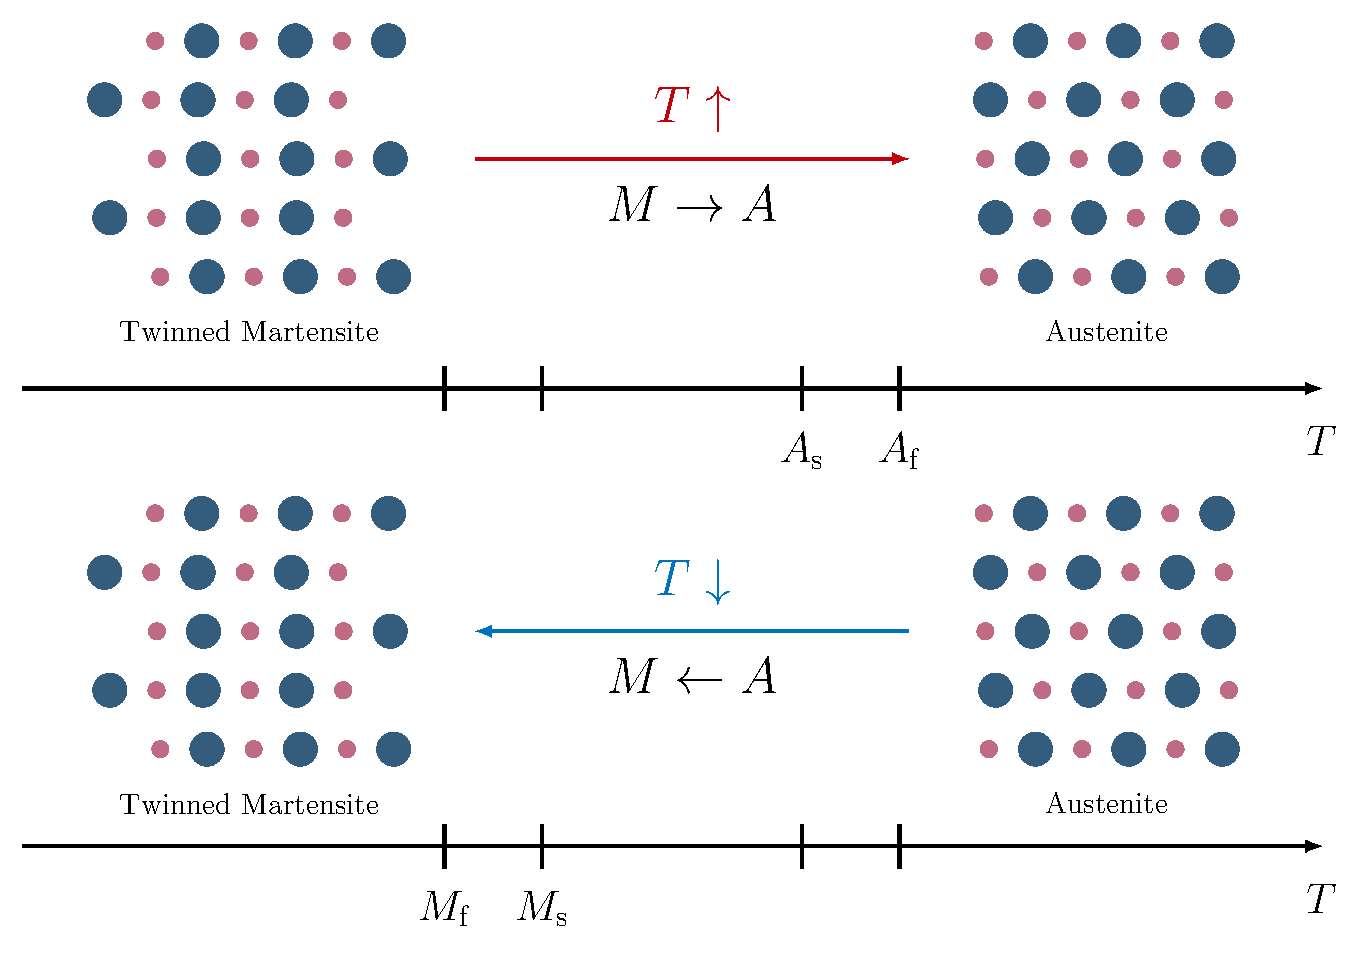
\includegraphics[width=0.75\textwidth]{images/chap2/sma-phase-transformations.pdf}
    \caption{A visual representation of the phase transformations that occur during Shape Memory Effect (SME) under no load adapted from the work by \cite{raoDesignShapeMemory2015}.}
    \label{fig:sma-phase-transformations}
\end{figure}

The SME was first reported in the work by \cite{changPlasticDeformationDiffusionless1951} in the 1950s. However, since then, there exists several different alloys that demonstrate the same interesting behaviour as shown in the work by \cite{WAYMAN19903}. The most commonly used alloy among these is the Ni-Ti alloy that was discovered at the US Naval Ordnance Laboratory in 1963 as thus, the alloy is often referred to as \textit{NiTiNOL}. In this work, the almost equiatomic Ni-Ti based SMA alloy is used due to its commercial availability in various different geometries and its excellent mechanical properties as shown in \cref{tab:niti-material-properties}. Furthermore, various additives and changes in atomic ratios can be used to change the transition temperatures threshold.

\begin{table}[hbt]
    \centering
    \caption{The material properties of Ni-Ti taken from the work by \cite{duerigTiNiShapeMemory1994} and \cite{raoDesignShapeMemory2015}}
    \label{tab:niti-material-properties}
    % !TEX root = ../../sethomas_thesis_main.tex
\documentclass[border=1mm,
               class=article
               preview]{standalone}

\begin{document}
\renewcommand{\arraystretch}{1.5}
 {\rowcolors{1}{black!5}{black!10}
\begin{tabular}{ll}
% \begin{tabular}{p{0.4\textwidth-2\tabcolsep}
%                 p{0.12\textwidth-2\tabcolsep}}
   \rowcolor{black} \textbf{\color{white} Material Property} & \textbf{\color{white} Value}\\
   Density [g/m$^3$] & 6.4-6.5\\
   Specific Heat [J/kg $^\circ$C] & 450-620\\
   Thermal Conductivity [W/m K] & 8.6-18\\
   Latent Heat [kJ/kg] & 19-32\\
   Electrical resistivity [$10^{-6}~\Omega$ m] & 0.5-1.1\\
   Thermal expansion coefficient [$10^{-6}~$K$^{-1}$] & 6.6-11\\
\end{tabular}}
\renewcommand{\arraystretch}{1}
\end{document}

\end{table}

\begin{figure}[hbt]
    \centering
    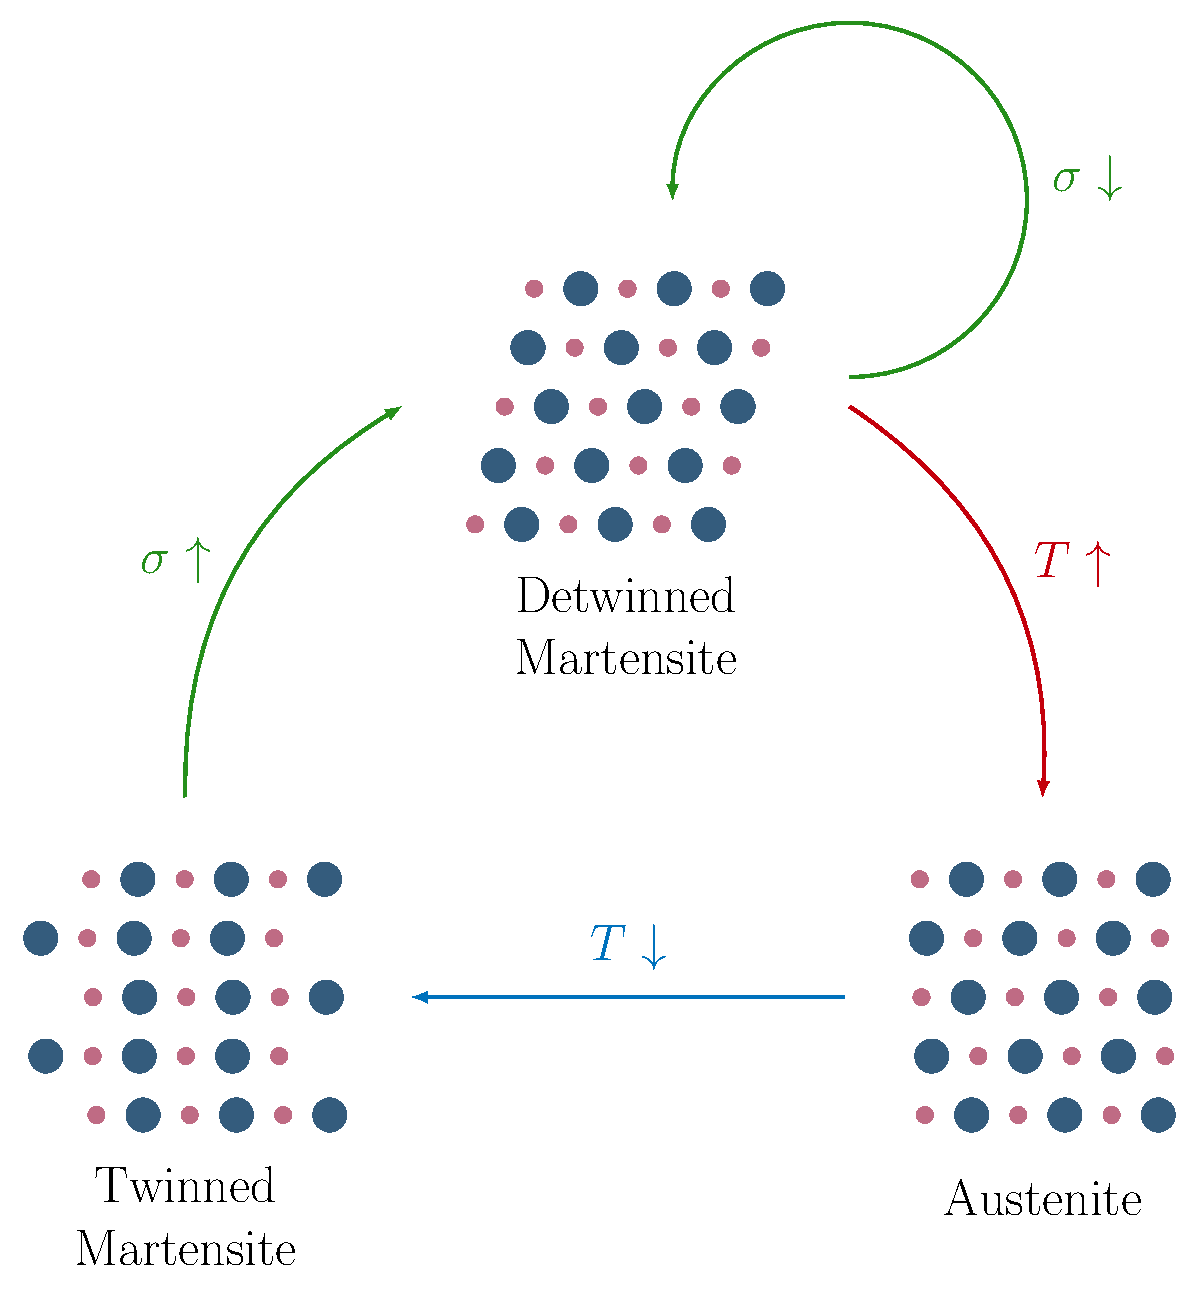
\includegraphics[width=0.6\textwidth]{images/chap2/sma-phases.pdf}
    \caption{A schematic representation of the Shape Memory Effect (SME) showing the different phase transformations and crystalline structures.}
    \label{fig:sma-phases}
\end{figure}

In \cref{fig:sma-phases}, the entire SME cycle can be observed along with the various changes in the phase and crystalline structures. At low temperature, the alloy exists in the twinned M phase. When subjected to a certain critical stress threshold, there are some shear lattice distortions that allow the material to be highly deformed ($\sim8$\%) and retain this strain. This effect is often referred to as detwinning and transforms the alloy to the detwinned M state. At high temperature, above a certain threshold, the alloy transforms into the A phase and the crystalline structures are restructured such that the material reverts back to its original shape before any mechanical loading. If the material is mechanically loaded in the A phase or by decreasing the transition temperature below the ambient temperature, any deformations imposed on the material is immediately recovered. This effect is known as Superelasticity or Pseudoelasticity (SE) as shown in the work by \cite{otsukaPseudoelasticityShapeMemory1986}. However, if the material is allowed to cool below the transition temperature, the alloy reverts back to the M phase where it can be deformed once again. This entire cycle is known as the SME and can be exploited to create highly compact and energy dense actuator. In \cref{fig:dsc-graph}, the required latent heat of transformation can be observed during the forward and backward transformations between the M and A phases. Often, as shown in the work by \cite{heDSCAnalysisReverse2004}, differential scanning calorimetry (DSC) can be used to accurately measure the transition temperature thresholds.

\begin{figure}[hbt]
    \centering
    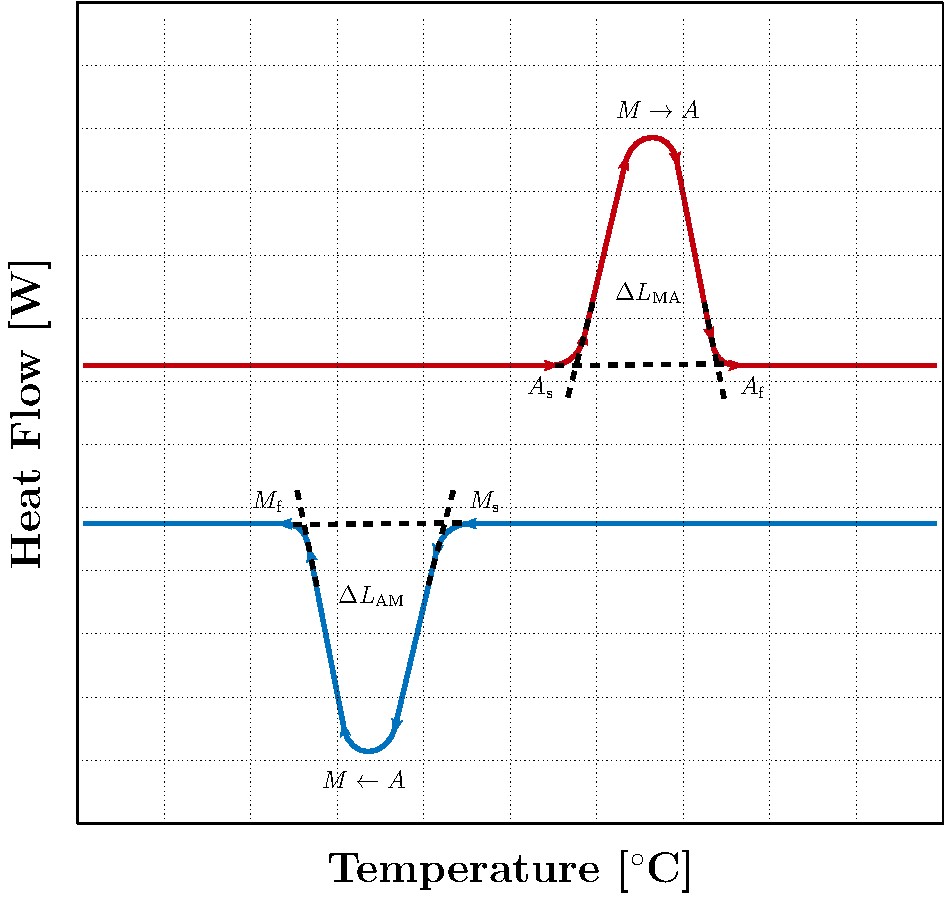
\includegraphics[width=0.75\textwidth]{images/chap2/dsc-graph.pdf}
    \caption{Schematic representation of a differential scanning calorimetry (DSC) graph showing the energy required during the SME where $\Delta L$ represents the latent heat of transformation between the two phases.}
    \label{fig:dsc-graph}
\end{figure}

As shown in the previous chapter, the main design criteria for SMA-based actuators is having a small footprint or being lightweight. Thus, when designing actuators, the active element and the biasing elements have to be perfectly balanced so that neither subsystems are oversized which results in wasted space or weight. Furthermore, as the cooling is often passive in SMA-powered actuators, employing larger SMA elements can exponentially decrease the bandwidth of the resulting actuator. The accurate sizing of the SMA element and biasing elements are, thus, critical in designing a compact and dynamic SMA actuator. In this chapter, various analytical and finite element method (FEM) models are presented so as to accurately predict the SME. Furthermore, using the developed models, various complex and simplified sizing methodology are described and presented such that the SMA can be adequately sized for any given application resulting in an energy dense actuator.

\section{Analytical Modelling of the SME}
% Phenomenological modelling
% DSC
% Types and history of models
% Brinson model
The Shape Memory Effect (SME) is a difficult process to model analytically due to the different phase transformations and interdependent variables. In the work by \cite{liangConstitutiveModelingShape1990a}, the authors presented a set of constitutive equations to describe a unified one-dimensional phenomenological model that incorporates the multi-physical nature of the SME and its internal variables. This model takes into account the phase transformations from the M and the A phases. The basic constitutive model presented by \cite{liangConstitutiveModelingShape1990a} is as follows,
\begin{equation}
  \label{eq:liang_model_1}
  d\sigma = \frac{\delta\sigma}{\delta\varepsilon}d\varepsilon + \frac{\delta\sigma}{\delta\xi}d\xi + \frac{\delta\sigma}{\delta T}dT
\end{equation}
\begin{equation}
  \label{eq:liang_model_2}
  d\sigma = Ed\varepsilon + \Omega d\xi + \Theta dT
\end{equation}
 which can be further simplified using constant material functions as
\begin{equation}
  \label{eq:liang_model_3}
  \sigma-\sigma_0 = E(\varepsilon-\varepsilon_0) + \Omega(\xi-\xi_0) + \Theta(T-T_0)
\end{equation}
where $E(\varepsilon,\xi,T)$ represents the Young's modulus of the SMA material, $\Omega(\varepsilon,\xi,T)$ represents the transformation tensor and $\Theta(\varepsilon,\xi,T)$ is the thermal coefficient of expansion of the SMA. Based on experimental evidence, as stated in the work by \cite{liangConstitutiveModelingShape1990a}, the Young's Modulus, $E$, of the SMA is directly proportional to the martensite fraction of the material. Thus, the following assumption is made to estimate the Young's modulus :
\begin{equation}
  \label{eq:youngs-modulus}
  E(\varepsilon,\xi,T) = E(\xi) = E_A + \xi(E_M-E_A)
\end{equation}
where, $E_A$ and $E_M$ represent the Young's modulus of the SMA when it is entirely in the Austenite phase or the Martensite phase, respectively. Furthermore, in the case of SMAs, a material limit must be imposed such that the maximum residual strain, $\varepsilon_L$ of the SME is incorporated into the model. This imposition creates a relationship between the Young's modulus and the transformation tensor :
\begin{equation}
  \label{eq:tensor-youngsmodulus}
  \Omega = -\varepsilon_L E
\end{equation}
In SMAs, the driving force that transforms the material from the A and M phases is the chemical free energy as a function of temperature and stress. In order to depict the martensite fraction as a function of stress and temperature during transformation, \cite{liangConstitutiveModelingShape1990a} developed an experimentally based cosine model, which fits well with experimental observations. The constitutive equations for the transformation from the A phase to the M phase, for $C_M(T-\Ms)<\sigma<C_M(T-\Mf)$, are described as follows:
\begin{equation}
  \label{eq:liang-MA}
  \xi=\frac{1-\xi_0}{2}cos\left[a_M\left(T-\Mf-\frac{\sigma}{C_M}\right)\right]+\frac{1+\xi_0}{2}
\end{equation}
while the reverse transformation, with $C_A(T-\Af)<\sigma<C_A(T-\As)$, from the M phase to the A phase is described as follows:
\begin{equation}
  \label{eq:liang-AM}
  \xi=\frac{\xi_0}{2}cos\left[a_A\left(T-\As-\frac{\sigma}{C_A}\right)\right]+\frac{\xi_0}{2}
\end{equation}
where $\xi_0$ represents the initial martensite fraction prior to the current transformation, $\sigma$ and $T$ is the current applied stress and temperature on the material, and $a_M$ and $a_A$ are expressed as follows:
\begin{equation}
  \label{eq:aM-aA}
  a_M=\frac{\pi}{\Ms-\Mf},~a_A=\frac{\pi}{\Af-\As}
\end{equation}
The material property $C_M$ and $C_A$, as shown in \cref{fig:phase-diagram-graph}, represent relationship between the critical stresses and transformation temperatures of the SMA. These constants are experimentally deduced and are considered linear as shown in the work by \cite{yooDevelopmentMartensiteTransformation2015}. These constants determine the critical stresses, $\sigma_\mathrm{cr}$ required to induce transformation or the determine the critical transformation temperatures at a certain imposed stress. The evolution of the martensite fraction based on the constitutive equations are shown in \cref{fig:sma-temperature-transformation-model}.
\begin{figure}[hbt]
    \centering
    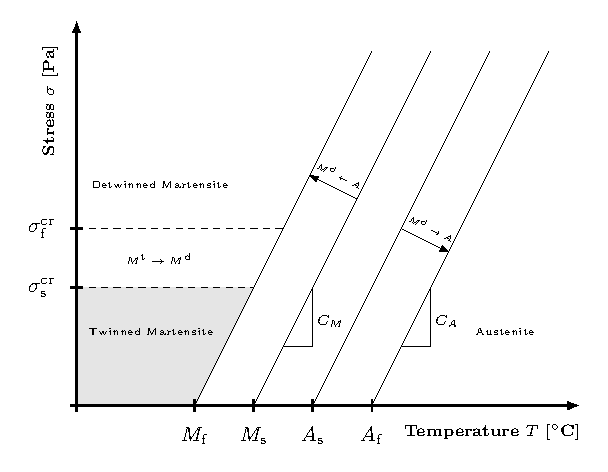
\includegraphics[width=0.75\textwidth]{images/chap2/phase-diagram-graph.pdf}
    \caption{Graphical representation of the phase transformations showing the thermal and mechanical properties of the material. This graph presents the change in the transformation temperature based on the imposed stress on the SMA adapted from the work by \cite{ricciardiChapterExperimentalCharacterization2021}}
    \label{fig:phase-diagram-graph}
\end{figure}

% Temp vs Martensite %
\begin{figure}[hbt]
    \centering
    \resizebox{0.75\textwidth}{!}{%% Creator: Matplotlib, PGF backend
%%
%% To include the figure in your LaTeX document, write
%%   \input{<filename>.pgf}
%%
%% Make sure the required packages are loaded in your preamble
%%   \usepackage{pgf}
%%
%% and, on pdftex
%%   \usepackage[utf8]{inputenc}\DeclareUnicodeCharacter{2212}{-}
%%
%% or, on luatex and xetex
%%   \usepackage{unicode-math}
%%
%% Figures using additional raster images can only be included by \input if
%% they are in the same directory as the main LaTeX file. For loading figures
%% from other directories you can use the `import` package
%%   \usepackage{import}
%%
%% and then include the figures with
%%   \import{<path to file>}{<filename>.pgf}
%%
%% Matplotlib used the following preamble
%%
\begingroup%
\makeatletter%
\begin{pgfpicture}%
\pgfpathrectangle{\pgfpointorigin}{\pgfqpoint{7.051524in}{4.502126in}}%
\pgfusepath{use as bounding box, clip}%
\begin{pgfscope}%
\pgfsetbuttcap%
\pgfsetmiterjoin%
\pgfsetlinewidth{0.000000pt}%
\definecolor{currentstroke}{rgb}{0.000000,0.000000,0.000000}%
\pgfsetstrokecolor{currentstroke}%
\pgfsetstrokeopacity{0.000000}%
\pgfsetdash{}{0pt}%
\pgfpathmoveto{\pgfqpoint{0.000000in}{0.000000in}}%
\pgfpathlineto{\pgfqpoint{7.051524in}{0.000000in}}%
\pgfpathlineto{\pgfqpoint{7.051524in}{4.502126in}}%
\pgfpathlineto{\pgfqpoint{0.000000in}{4.502126in}}%
\pgfpathclose%
\pgfusepath{}%
\end{pgfscope}%
\begin{pgfscope}%
\pgfsetbuttcap%
\pgfsetmiterjoin%
\pgfsetlinewidth{0.000000pt}%
\definecolor{currentstroke}{rgb}{0.000000,0.000000,0.000000}%
\pgfsetstrokecolor{currentstroke}%
\pgfsetstrokeopacity{0.000000}%
\pgfsetdash{}{0pt}%
\pgfpathmoveto{\pgfqpoint{0.751524in}{0.706126in}}%
\pgfpathlineto{\pgfqpoint{6.951524in}{0.706126in}}%
\pgfpathlineto{\pgfqpoint{6.951524in}{4.402126in}}%
\pgfpathlineto{\pgfqpoint{0.751524in}{4.402126in}}%
\pgfpathclose%
\pgfusepath{}%
\end{pgfscope}%
\begin{pgfscope}%
\pgfpathrectangle{\pgfqpoint{0.751524in}{0.706126in}}{\pgfqpoint{6.200000in}{3.696000in}}%
\pgfusepath{clip}%
\pgfsetbuttcap%
\pgfsetroundjoin%
\pgfsetlinewidth{0.803000pt}%
\definecolor{currentstroke}{rgb}{0.690196,0.690196,0.690196}%
\pgfsetstrokecolor{currentstroke}%
\pgfsetstrokeopacity{0.750000}%
\pgfsetdash{{0.800000pt}{1.320000pt}}{0.000000pt}%
\pgfpathmoveto{\pgfqpoint{2.160615in}{0.706126in}}%
\pgfpathlineto{\pgfqpoint{2.160615in}{4.402126in}}%
\pgfusepath{stroke}%
\end{pgfscope}%
\begin{pgfscope}%
\pgfsetbuttcap%
\pgfsetroundjoin%
\definecolor{currentfill}{rgb}{0.000000,0.000000,0.000000}%
\pgfsetfillcolor{currentfill}%
\pgfsetlinewidth{0.803000pt}%
\definecolor{currentstroke}{rgb}{0.000000,0.000000,0.000000}%
\pgfsetstrokecolor{currentstroke}%
\pgfsetdash{}{0pt}%
\pgfsys@defobject{currentmarker}{\pgfqpoint{0.000000in}{-0.048611in}}{\pgfqpoint{0.000000in}{0.000000in}}{%
\pgfpathmoveto{\pgfqpoint{0.000000in}{0.000000in}}%
\pgfpathlineto{\pgfqpoint{0.000000in}{-0.048611in}}%
\pgfusepath{stroke,fill}%
}%
\begin{pgfscope}%
\pgfsys@transformshift{2.160615in}{0.706126in}%
\pgfsys@useobject{currentmarker}{}%
\end{pgfscope}%
\end{pgfscope}%
\begin{pgfscope}%
\definecolor{textcolor}{rgb}{0.000000,0.000000,0.000000}%
\pgfsetstrokecolor{textcolor}%
\pgfsetfillcolor{textcolor}%
\pgftext[x=2.160615in,y=0.608904in,,top]{\color{textcolor}\rmfamily\fontsize{16.000000}{19.200000}\selectfont \(\displaystyle M_{\mathrm{f}}\)}%
\end{pgfscope}%
\begin{pgfscope}%
\pgfpathrectangle{\pgfqpoint{0.751524in}{0.706126in}}{\pgfqpoint{6.200000in}{3.696000in}}%
\pgfusepath{clip}%
\pgfsetbuttcap%
\pgfsetroundjoin%
\pgfsetlinewidth{0.803000pt}%
\definecolor{currentstroke}{rgb}{0.690196,0.690196,0.690196}%
\pgfsetstrokecolor{currentstroke}%
\pgfsetstrokeopacity{0.750000}%
\pgfsetdash{{0.800000pt}{1.320000pt}}{0.000000pt}%
\pgfpathmoveto{\pgfqpoint{3.287888in}{0.706126in}}%
\pgfpathlineto{\pgfqpoint{3.287888in}{4.402126in}}%
\pgfusepath{stroke}%
\end{pgfscope}%
\begin{pgfscope}%
\pgfsetbuttcap%
\pgfsetroundjoin%
\definecolor{currentfill}{rgb}{0.000000,0.000000,0.000000}%
\pgfsetfillcolor{currentfill}%
\pgfsetlinewidth{0.803000pt}%
\definecolor{currentstroke}{rgb}{0.000000,0.000000,0.000000}%
\pgfsetstrokecolor{currentstroke}%
\pgfsetdash{}{0pt}%
\pgfsys@defobject{currentmarker}{\pgfqpoint{0.000000in}{-0.048611in}}{\pgfqpoint{0.000000in}{0.000000in}}{%
\pgfpathmoveto{\pgfqpoint{0.000000in}{0.000000in}}%
\pgfpathlineto{\pgfqpoint{0.000000in}{-0.048611in}}%
\pgfusepath{stroke,fill}%
}%
\begin{pgfscope}%
\pgfsys@transformshift{3.287888in}{0.706126in}%
\pgfsys@useobject{currentmarker}{}%
\end{pgfscope}%
\end{pgfscope}%
\begin{pgfscope}%
\definecolor{textcolor}{rgb}{0.000000,0.000000,0.000000}%
\pgfsetstrokecolor{textcolor}%
\pgfsetfillcolor{textcolor}%
\pgftext[x=3.287888in,y=0.608904in,,top]{\color{textcolor}\rmfamily\fontsize{16.000000}{19.200000}\selectfont \(\displaystyle M_{\mathrm{s}}\)}%
\end{pgfscope}%
\begin{pgfscope}%
\pgfpathrectangle{\pgfqpoint{0.751524in}{0.706126in}}{\pgfqpoint{6.200000in}{3.696000in}}%
\pgfusepath{clip}%
\pgfsetbuttcap%
\pgfsetroundjoin%
\pgfsetlinewidth{0.803000pt}%
\definecolor{currentstroke}{rgb}{0.690196,0.690196,0.690196}%
\pgfsetstrokecolor{currentstroke}%
\pgfsetstrokeopacity{0.750000}%
\pgfsetdash{{0.800000pt}{1.320000pt}}{0.000000pt}%
\pgfpathmoveto{\pgfqpoint{4.415160in}{0.706126in}}%
\pgfpathlineto{\pgfqpoint{4.415160in}{4.402126in}}%
\pgfusepath{stroke}%
\end{pgfscope}%
\begin{pgfscope}%
\pgfsetbuttcap%
\pgfsetroundjoin%
\definecolor{currentfill}{rgb}{0.000000,0.000000,0.000000}%
\pgfsetfillcolor{currentfill}%
\pgfsetlinewidth{0.803000pt}%
\definecolor{currentstroke}{rgb}{0.000000,0.000000,0.000000}%
\pgfsetstrokecolor{currentstroke}%
\pgfsetdash{}{0pt}%
\pgfsys@defobject{currentmarker}{\pgfqpoint{0.000000in}{-0.048611in}}{\pgfqpoint{0.000000in}{0.000000in}}{%
\pgfpathmoveto{\pgfqpoint{0.000000in}{0.000000in}}%
\pgfpathlineto{\pgfqpoint{0.000000in}{-0.048611in}}%
\pgfusepath{stroke,fill}%
}%
\begin{pgfscope}%
\pgfsys@transformshift{4.415160in}{0.706126in}%
\pgfsys@useobject{currentmarker}{}%
\end{pgfscope}%
\end{pgfscope}%
\begin{pgfscope}%
\definecolor{textcolor}{rgb}{0.000000,0.000000,0.000000}%
\pgfsetstrokecolor{textcolor}%
\pgfsetfillcolor{textcolor}%
\pgftext[x=4.415160in,y=0.608904in,,top]{\color{textcolor}\rmfamily\fontsize{16.000000}{19.200000}\selectfont \(\displaystyle A_{\mathrm{s}}\)}%
\end{pgfscope}%
\begin{pgfscope}%
\pgfpathrectangle{\pgfqpoint{0.751524in}{0.706126in}}{\pgfqpoint{6.200000in}{3.696000in}}%
\pgfusepath{clip}%
\pgfsetbuttcap%
\pgfsetroundjoin%
\pgfsetlinewidth{0.803000pt}%
\definecolor{currentstroke}{rgb}{0.690196,0.690196,0.690196}%
\pgfsetstrokecolor{currentstroke}%
\pgfsetstrokeopacity{0.750000}%
\pgfsetdash{{0.800000pt}{1.320000pt}}{0.000000pt}%
\pgfpathmoveto{\pgfqpoint{5.542433in}{0.706126in}}%
\pgfpathlineto{\pgfqpoint{5.542433in}{4.402126in}}%
\pgfusepath{stroke}%
\end{pgfscope}%
\begin{pgfscope}%
\pgfsetbuttcap%
\pgfsetroundjoin%
\definecolor{currentfill}{rgb}{0.000000,0.000000,0.000000}%
\pgfsetfillcolor{currentfill}%
\pgfsetlinewidth{0.803000pt}%
\definecolor{currentstroke}{rgb}{0.000000,0.000000,0.000000}%
\pgfsetstrokecolor{currentstroke}%
\pgfsetdash{}{0pt}%
\pgfsys@defobject{currentmarker}{\pgfqpoint{0.000000in}{-0.048611in}}{\pgfqpoint{0.000000in}{0.000000in}}{%
\pgfpathmoveto{\pgfqpoint{0.000000in}{0.000000in}}%
\pgfpathlineto{\pgfqpoint{0.000000in}{-0.048611in}}%
\pgfusepath{stroke,fill}%
}%
\begin{pgfscope}%
\pgfsys@transformshift{5.542433in}{0.706126in}%
\pgfsys@useobject{currentmarker}{}%
\end{pgfscope}%
\end{pgfscope}%
\begin{pgfscope}%
\definecolor{textcolor}{rgb}{0.000000,0.000000,0.000000}%
\pgfsetstrokecolor{textcolor}%
\pgfsetfillcolor{textcolor}%
\pgftext[x=5.542433in,y=0.608904in,,top]{\color{textcolor}\rmfamily\fontsize{16.000000}{19.200000}\selectfont \(\displaystyle A_{\mathrm{f}}\)}%
\end{pgfscope}%
\begin{pgfscope}%
\definecolor{textcolor}{rgb}{0.000000,0.000000,0.000000}%
\pgfsetstrokecolor{textcolor}%
\pgfsetfillcolor{textcolor}%
\pgftext[x=3.851524in,y=0.340000in,,top]{\color{textcolor}\rmfamily\fontsize{16.000000}{19.200000}\bfseries\selectfont Temperature \(\displaystyle T\) [\(\displaystyle ^\circ\)C]}%
\end{pgfscope}%
\begin{pgfscope}%
\pgfpathrectangle{\pgfqpoint{0.751524in}{0.706126in}}{\pgfqpoint{6.200000in}{3.696000in}}%
\pgfusepath{clip}%
\pgfsetbuttcap%
\pgfsetroundjoin%
\pgfsetlinewidth{0.803000pt}%
\definecolor{currentstroke}{rgb}{0.690196,0.690196,0.690196}%
\pgfsetstrokecolor{currentstroke}%
\pgfsetstrokeopacity{0.750000}%
\pgfsetdash{{0.800000pt}{1.320000pt}}{0.000000pt}%
\pgfpathmoveto{\pgfqpoint{0.751524in}{0.874126in}}%
\pgfpathlineto{\pgfqpoint{6.951524in}{0.874126in}}%
\pgfusepath{stroke}%
\end{pgfscope}%
\begin{pgfscope}%
\pgfsetbuttcap%
\pgfsetroundjoin%
\definecolor{currentfill}{rgb}{0.000000,0.000000,0.000000}%
\pgfsetfillcolor{currentfill}%
\pgfsetlinewidth{0.803000pt}%
\definecolor{currentstroke}{rgb}{0.000000,0.000000,0.000000}%
\pgfsetstrokecolor{currentstroke}%
\pgfsetdash{}{0pt}%
\pgfsys@defobject{currentmarker}{\pgfqpoint{-0.048611in}{0.000000in}}{\pgfqpoint{-0.000000in}{0.000000in}}{%
\pgfpathmoveto{\pgfqpoint{-0.000000in}{0.000000in}}%
\pgfpathlineto{\pgfqpoint{-0.048611in}{0.000000in}}%
\pgfusepath{stroke,fill}%
}%
\begin{pgfscope}%
\pgfsys@transformshift{0.751524in}{0.874126in}%
\pgfsys@useobject{currentmarker}{}%
\end{pgfscope}%
\end{pgfscope}%
\begin{pgfscope}%
\definecolor{textcolor}{rgb}{0.000000,0.000000,0.000000}%
\pgfsetstrokecolor{textcolor}%
\pgfsetfillcolor{textcolor}%
\pgftext[x=0.368888in, y=0.790793in, left, base]{\color{textcolor}\rmfamily\fontsize{16.000000}{19.200000}\selectfont \(\displaystyle {0.0}\)}%
\end{pgfscope}%
\begin{pgfscope}%
\pgfpathrectangle{\pgfqpoint{0.751524in}{0.706126in}}{\pgfqpoint{6.200000in}{3.696000in}}%
\pgfusepath{clip}%
\pgfsetbuttcap%
\pgfsetroundjoin%
\pgfsetlinewidth{0.803000pt}%
\definecolor{currentstroke}{rgb}{0.690196,0.690196,0.690196}%
\pgfsetstrokecolor{currentstroke}%
\pgfsetstrokeopacity{0.750000}%
\pgfsetdash{{0.800000pt}{1.320000pt}}{0.000000pt}%
\pgfpathmoveto{\pgfqpoint{0.751524in}{1.546126in}}%
\pgfpathlineto{\pgfqpoint{6.951524in}{1.546126in}}%
\pgfusepath{stroke}%
\end{pgfscope}%
\begin{pgfscope}%
\pgfsetbuttcap%
\pgfsetroundjoin%
\definecolor{currentfill}{rgb}{0.000000,0.000000,0.000000}%
\pgfsetfillcolor{currentfill}%
\pgfsetlinewidth{0.803000pt}%
\definecolor{currentstroke}{rgb}{0.000000,0.000000,0.000000}%
\pgfsetstrokecolor{currentstroke}%
\pgfsetdash{}{0pt}%
\pgfsys@defobject{currentmarker}{\pgfqpoint{-0.048611in}{0.000000in}}{\pgfqpoint{-0.000000in}{0.000000in}}{%
\pgfpathmoveto{\pgfqpoint{-0.000000in}{0.000000in}}%
\pgfpathlineto{\pgfqpoint{-0.048611in}{0.000000in}}%
\pgfusepath{stroke,fill}%
}%
\begin{pgfscope}%
\pgfsys@transformshift{0.751524in}{1.546126in}%
\pgfsys@useobject{currentmarker}{}%
\end{pgfscope}%
\end{pgfscope}%
\begin{pgfscope}%
\definecolor{textcolor}{rgb}{0.000000,0.000000,0.000000}%
\pgfsetstrokecolor{textcolor}%
\pgfsetfillcolor{textcolor}%
\pgftext[x=0.368888in, y=1.462793in, left, base]{\color{textcolor}\rmfamily\fontsize{16.000000}{19.200000}\selectfont \(\displaystyle {0.2}\)}%
\end{pgfscope}%
\begin{pgfscope}%
\pgfpathrectangle{\pgfqpoint{0.751524in}{0.706126in}}{\pgfqpoint{6.200000in}{3.696000in}}%
\pgfusepath{clip}%
\pgfsetbuttcap%
\pgfsetroundjoin%
\pgfsetlinewidth{0.803000pt}%
\definecolor{currentstroke}{rgb}{0.690196,0.690196,0.690196}%
\pgfsetstrokecolor{currentstroke}%
\pgfsetstrokeopacity{0.750000}%
\pgfsetdash{{0.800000pt}{1.320000pt}}{0.000000pt}%
\pgfpathmoveto{\pgfqpoint{0.751524in}{2.218126in}}%
\pgfpathlineto{\pgfqpoint{6.951524in}{2.218126in}}%
\pgfusepath{stroke}%
\end{pgfscope}%
\begin{pgfscope}%
\pgfsetbuttcap%
\pgfsetroundjoin%
\definecolor{currentfill}{rgb}{0.000000,0.000000,0.000000}%
\pgfsetfillcolor{currentfill}%
\pgfsetlinewidth{0.803000pt}%
\definecolor{currentstroke}{rgb}{0.000000,0.000000,0.000000}%
\pgfsetstrokecolor{currentstroke}%
\pgfsetdash{}{0pt}%
\pgfsys@defobject{currentmarker}{\pgfqpoint{-0.048611in}{0.000000in}}{\pgfqpoint{-0.000000in}{0.000000in}}{%
\pgfpathmoveto{\pgfqpoint{-0.000000in}{0.000000in}}%
\pgfpathlineto{\pgfqpoint{-0.048611in}{0.000000in}}%
\pgfusepath{stroke,fill}%
}%
\begin{pgfscope}%
\pgfsys@transformshift{0.751524in}{2.218126in}%
\pgfsys@useobject{currentmarker}{}%
\end{pgfscope}%
\end{pgfscope}%
\begin{pgfscope}%
\definecolor{textcolor}{rgb}{0.000000,0.000000,0.000000}%
\pgfsetstrokecolor{textcolor}%
\pgfsetfillcolor{textcolor}%
\pgftext[x=0.368888in, y=2.134793in, left, base]{\color{textcolor}\rmfamily\fontsize{16.000000}{19.200000}\selectfont \(\displaystyle {0.4}\)}%
\end{pgfscope}%
\begin{pgfscope}%
\pgfpathrectangle{\pgfqpoint{0.751524in}{0.706126in}}{\pgfqpoint{6.200000in}{3.696000in}}%
\pgfusepath{clip}%
\pgfsetbuttcap%
\pgfsetroundjoin%
\pgfsetlinewidth{0.803000pt}%
\definecolor{currentstroke}{rgb}{0.690196,0.690196,0.690196}%
\pgfsetstrokecolor{currentstroke}%
\pgfsetstrokeopacity{0.750000}%
\pgfsetdash{{0.800000pt}{1.320000pt}}{0.000000pt}%
\pgfpathmoveto{\pgfqpoint{0.751524in}{2.890126in}}%
\pgfpathlineto{\pgfqpoint{6.951524in}{2.890126in}}%
\pgfusepath{stroke}%
\end{pgfscope}%
\begin{pgfscope}%
\pgfsetbuttcap%
\pgfsetroundjoin%
\definecolor{currentfill}{rgb}{0.000000,0.000000,0.000000}%
\pgfsetfillcolor{currentfill}%
\pgfsetlinewidth{0.803000pt}%
\definecolor{currentstroke}{rgb}{0.000000,0.000000,0.000000}%
\pgfsetstrokecolor{currentstroke}%
\pgfsetdash{}{0pt}%
\pgfsys@defobject{currentmarker}{\pgfqpoint{-0.048611in}{0.000000in}}{\pgfqpoint{-0.000000in}{0.000000in}}{%
\pgfpathmoveto{\pgfqpoint{-0.000000in}{0.000000in}}%
\pgfpathlineto{\pgfqpoint{-0.048611in}{0.000000in}}%
\pgfusepath{stroke,fill}%
}%
\begin{pgfscope}%
\pgfsys@transformshift{0.751524in}{2.890126in}%
\pgfsys@useobject{currentmarker}{}%
\end{pgfscope}%
\end{pgfscope}%
\begin{pgfscope}%
\definecolor{textcolor}{rgb}{0.000000,0.000000,0.000000}%
\pgfsetstrokecolor{textcolor}%
\pgfsetfillcolor{textcolor}%
\pgftext[x=0.368888in, y=2.806793in, left, base]{\color{textcolor}\rmfamily\fontsize{16.000000}{19.200000}\selectfont \(\displaystyle {0.6}\)}%
\end{pgfscope}%
\begin{pgfscope}%
\pgfpathrectangle{\pgfqpoint{0.751524in}{0.706126in}}{\pgfqpoint{6.200000in}{3.696000in}}%
\pgfusepath{clip}%
\pgfsetbuttcap%
\pgfsetroundjoin%
\pgfsetlinewidth{0.803000pt}%
\definecolor{currentstroke}{rgb}{0.690196,0.690196,0.690196}%
\pgfsetstrokecolor{currentstroke}%
\pgfsetstrokeopacity{0.750000}%
\pgfsetdash{{0.800000pt}{1.320000pt}}{0.000000pt}%
\pgfpathmoveto{\pgfqpoint{0.751524in}{3.562126in}}%
\pgfpathlineto{\pgfqpoint{6.951524in}{3.562126in}}%
\pgfusepath{stroke}%
\end{pgfscope}%
\begin{pgfscope}%
\pgfsetbuttcap%
\pgfsetroundjoin%
\definecolor{currentfill}{rgb}{0.000000,0.000000,0.000000}%
\pgfsetfillcolor{currentfill}%
\pgfsetlinewidth{0.803000pt}%
\definecolor{currentstroke}{rgb}{0.000000,0.000000,0.000000}%
\pgfsetstrokecolor{currentstroke}%
\pgfsetdash{}{0pt}%
\pgfsys@defobject{currentmarker}{\pgfqpoint{-0.048611in}{0.000000in}}{\pgfqpoint{-0.000000in}{0.000000in}}{%
\pgfpathmoveto{\pgfqpoint{-0.000000in}{0.000000in}}%
\pgfpathlineto{\pgfqpoint{-0.048611in}{0.000000in}}%
\pgfusepath{stroke,fill}%
}%
\begin{pgfscope}%
\pgfsys@transformshift{0.751524in}{3.562126in}%
\pgfsys@useobject{currentmarker}{}%
\end{pgfscope}%
\end{pgfscope}%
\begin{pgfscope}%
\definecolor{textcolor}{rgb}{0.000000,0.000000,0.000000}%
\pgfsetstrokecolor{textcolor}%
\pgfsetfillcolor{textcolor}%
\pgftext[x=0.368888in, y=3.478793in, left, base]{\color{textcolor}\rmfamily\fontsize{16.000000}{19.200000}\selectfont \(\displaystyle {0.8}\)}%
\end{pgfscope}%
\begin{pgfscope}%
\pgfpathrectangle{\pgfqpoint{0.751524in}{0.706126in}}{\pgfqpoint{6.200000in}{3.696000in}}%
\pgfusepath{clip}%
\pgfsetbuttcap%
\pgfsetroundjoin%
\pgfsetlinewidth{0.803000pt}%
\definecolor{currentstroke}{rgb}{0.690196,0.690196,0.690196}%
\pgfsetstrokecolor{currentstroke}%
\pgfsetstrokeopacity{0.750000}%
\pgfsetdash{{0.800000pt}{1.320000pt}}{0.000000pt}%
\pgfpathmoveto{\pgfqpoint{0.751524in}{4.234126in}}%
\pgfpathlineto{\pgfqpoint{6.951524in}{4.234126in}}%
\pgfusepath{stroke}%
\end{pgfscope}%
\begin{pgfscope}%
\pgfsetbuttcap%
\pgfsetroundjoin%
\definecolor{currentfill}{rgb}{0.000000,0.000000,0.000000}%
\pgfsetfillcolor{currentfill}%
\pgfsetlinewidth{0.803000pt}%
\definecolor{currentstroke}{rgb}{0.000000,0.000000,0.000000}%
\pgfsetstrokecolor{currentstroke}%
\pgfsetdash{}{0pt}%
\pgfsys@defobject{currentmarker}{\pgfqpoint{-0.048611in}{0.000000in}}{\pgfqpoint{-0.000000in}{0.000000in}}{%
\pgfpathmoveto{\pgfqpoint{-0.000000in}{0.000000in}}%
\pgfpathlineto{\pgfqpoint{-0.048611in}{0.000000in}}%
\pgfusepath{stroke,fill}%
}%
\begin{pgfscope}%
\pgfsys@transformshift{0.751524in}{4.234126in}%
\pgfsys@useobject{currentmarker}{}%
\end{pgfscope}%
\end{pgfscope}%
\begin{pgfscope}%
\definecolor{textcolor}{rgb}{0.000000,0.000000,0.000000}%
\pgfsetstrokecolor{textcolor}%
\pgfsetfillcolor{textcolor}%
\pgftext[x=0.368888in, y=4.150793in, left, base]{\color{textcolor}\rmfamily\fontsize{16.000000}{19.200000}\selectfont \(\displaystyle {1.0}\)}%
\end{pgfscope}%
\begin{pgfscope}%
\definecolor{textcolor}{rgb}{0.000000,0.000000,0.000000}%
\pgfsetstrokecolor{textcolor}%
\pgfsetfillcolor{textcolor}%
\pgftext[x=0.313333in,y=2.554126in,,bottom,rotate=90.000000]{\color{textcolor}\rmfamily\fontsize{16.000000}{19.200000}\bfseries\selectfont Martensite Fraction \(\displaystyle \xi\)}%
\end{pgfscope}%
\begin{pgfscope}%
\pgfpathrectangle{\pgfqpoint{0.751524in}{0.706126in}}{\pgfqpoint{6.200000in}{3.696000in}}%
\pgfusepath{clip}%
\pgfsetrectcap%
\pgfsetroundjoin%
\pgfsetlinewidth{1.505625pt}%
\definecolor{currentstroke}{rgb}{0.000000,0.447059,0.741176}%
\pgfsetstrokecolor{currentstroke}%
\pgfsetdash{}{0pt}%
\pgfpathmoveto{\pgfqpoint{6.669706in}{0.874126in}}%
\pgfpathlineto{\pgfqpoint{6.612773in}{0.874126in}}%
\pgfpathlineto{\pgfqpoint{6.555840in}{0.874126in}}%
\pgfpathlineto{\pgfqpoint{6.498907in}{0.874126in}}%
\pgfpathlineto{\pgfqpoint{6.441974in}{0.874126in}}%
\pgfpathlineto{\pgfqpoint{6.385041in}{0.874126in}}%
\pgfpathlineto{\pgfqpoint{6.328108in}{0.874126in}}%
\pgfpathlineto{\pgfqpoint{6.271175in}{0.874126in}}%
\pgfpathlineto{\pgfqpoint{6.214242in}{0.874126in}}%
\pgfpathlineto{\pgfqpoint{6.157309in}{0.874126in}}%
\pgfpathlineto{\pgfqpoint{6.100376in}{0.874126in}}%
\pgfpathlineto{\pgfqpoint{6.043443in}{0.874126in}}%
\pgfpathlineto{\pgfqpoint{5.986510in}{0.874126in}}%
\pgfpathlineto{\pgfqpoint{5.929577in}{0.874126in}}%
\pgfpathlineto{\pgfqpoint{5.872644in}{0.874126in}}%
\pgfpathlineto{\pgfqpoint{5.815711in}{0.874126in}}%
\pgfpathlineto{\pgfqpoint{5.758778in}{0.874126in}}%
\pgfpathlineto{\pgfqpoint{5.701845in}{0.874126in}}%
\pgfpathlineto{\pgfqpoint{5.644912in}{0.874126in}}%
\pgfpathlineto{\pgfqpoint{5.587979in}{0.874126in}}%
\pgfpathlineto{\pgfqpoint{5.531047in}{0.874126in}}%
\pgfpathlineto{\pgfqpoint{5.474114in}{0.874126in}}%
\pgfpathlineto{\pgfqpoint{5.417181in}{0.874126in}}%
\pgfpathlineto{\pgfqpoint{5.360248in}{0.874126in}}%
\pgfpathlineto{\pgfqpoint{5.303315in}{0.874126in}}%
\pgfpathlineto{\pgfqpoint{5.246382in}{0.874126in}}%
\pgfpathlineto{\pgfqpoint{5.189449in}{0.874126in}}%
\pgfpathlineto{\pgfqpoint{5.132516in}{0.874126in}}%
\pgfpathlineto{\pgfqpoint{5.075583in}{0.874126in}}%
\pgfpathlineto{\pgfqpoint{5.018650in}{0.874126in}}%
\pgfpathlineto{\pgfqpoint{4.961717in}{0.874126in}}%
\pgfpathlineto{\pgfqpoint{4.904784in}{0.874126in}}%
\pgfpathlineto{\pgfqpoint{4.847851in}{0.874126in}}%
\pgfpathlineto{\pgfqpoint{4.790918in}{0.874126in}}%
\pgfpathlineto{\pgfqpoint{4.733985in}{0.874126in}}%
\pgfpathlineto{\pgfqpoint{4.677052in}{0.874126in}}%
\pgfpathlineto{\pgfqpoint{4.620119in}{0.874126in}}%
\pgfpathlineto{\pgfqpoint{4.563186in}{0.874126in}}%
\pgfpathlineto{\pgfqpoint{4.506253in}{0.874126in}}%
\pgfpathlineto{\pgfqpoint{4.449320in}{0.874126in}}%
\pgfpathlineto{\pgfqpoint{4.392387in}{0.874126in}}%
\pgfpathlineto{\pgfqpoint{4.335454in}{0.874126in}}%
\pgfpathlineto{\pgfqpoint{4.278521in}{0.874126in}}%
\pgfpathlineto{\pgfqpoint{4.221588in}{0.874126in}}%
\pgfpathlineto{\pgfqpoint{4.164655in}{0.874126in}}%
\pgfpathlineto{\pgfqpoint{4.107722in}{0.874126in}}%
\pgfpathlineto{\pgfqpoint{4.050789in}{0.874126in}}%
\pgfpathlineto{\pgfqpoint{3.993856in}{0.874126in}}%
\pgfpathlineto{\pgfqpoint{3.936923in}{0.874126in}}%
\pgfpathlineto{\pgfqpoint{3.879991in}{0.874126in}}%
\pgfpathlineto{\pgfqpoint{3.823058in}{0.874126in}}%
\pgfpathlineto{\pgfqpoint{3.766125in}{0.874126in}}%
\pgfpathlineto{\pgfqpoint{3.709192in}{0.874126in}}%
\pgfpathlineto{\pgfqpoint{3.652259in}{0.874126in}}%
\pgfpathlineto{\pgfqpoint{3.595326in}{0.874126in}}%
\pgfpathlineto{\pgfqpoint{3.538393in}{0.874126in}}%
\pgfpathlineto{\pgfqpoint{3.481460in}{0.874126in}}%
\pgfpathlineto{\pgfqpoint{3.424527in}{0.874126in}}%
\pgfpathlineto{\pgfqpoint{3.367594in}{0.874126in}}%
\pgfpathlineto{\pgfqpoint{3.310661in}{0.874126in}}%
\pgfpathlineto{\pgfqpoint{3.253728in}{0.881733in}}%
\pgfpathlineto{\pgfqpoint{3.196795in}{0.927972in}}%
\pgfpathlineto{\pgfqpoint{3.139862in}{1.015064in}}%
\pgfpathlineto{\pgfqpoint{3.082929in}{1.140820in}}%
\pgfpathlineto{\pgfqpoint{3.025996in}{1.302082in}}%
\pgfpathlineto{\pgfqpoint{2.969063in}{1.494798in}}%
\pgfpathlineto{\pgfqpoint{2.912130in}{1.714126in}}%
\pgfpathlineto{\pgfqpoint{2.855197in}{1.954557in}}%
\pgfpathlineto{\pgfqpoint{2.798264in}{2.210051in}}%
\pgfpathlineto{\pgfqpoint{2.741331in}{2.474188in}}%
\pgfpathlineto{\pgfqpoint{2.684398in}{2.740334in}}%
\pgfpathlineto{\pgfqpoint{2.627465in}{3.001802in}}%
\pgfpathlineto{\pgfqpoint{2.570532in}{3.252023in}}%
\pgfpathlineto{\pgfqpoint{2.513599in}{3.484712in}}%
\pgfpathlineto{\pgfqpoint{2.456666in}{3.694022in}}%
\pgfpathlineto{\pgfqpoint{2.399733in}{3.874695in}}%
\pgfpathlineto{\pgfqpoint{2.342800in}{4.022193in}}%
\pgfpathlineto{\pgfqpoint{2.285867in}{4.132810in}}%
\pgfpathlineto{\pgfqpoint{2.228934in}{4.203766in}}%
\pgfpathlineto{\pgfqpoint{2.172002in}{4.233280in}}%
\pgfpathlineto{\pgfqpoint{2.115069in}{4.234126in}}%
\pgfpathlineto{\pgfqpoint{2.058136in}{4.234126in}}%
\pgfpathlineto{\pgfqpoint{2.001203in}{4.234126in}}%
\pgfpathlineto{\pgfqpoint{1.944270in}{4.234126in}}%
\pgfpathlineto{\pgfqpoint{1.887337in}{4.234126in}}%
\pgfpathlineto{\pgfqpoint{1.830404in}{4.234126in}}%
\pgfpathlineto{\pgfqpoint{1.773471in}{4.234126in}}%
\pgfpathlineto{\pgfqpoint{1.716538in}{4.234126in}}%
\pgfpathlineto{\pgfqpoint{1.659605in}{4.234126in}}%
\pgfpathlineto{\pgfqpoint{1.602672in}{4.234126in}}%
\pgfpathlineto{\pgfqpoint{1.545739in}{4.234126in}}%
\pgfpathlineto{\pgfqpoint{1.488806in}{4.234126in}}%
\pgfpathlineto{\pgfqpoint{1.431873in}{4.234126in}}%
\pgfpathlineto{\pgfqpoint{1.374940in}{4.234126in}}%
\pgfpathlineto{\pgfqpoint{1.318007in}{4.234126in}}%
\pgfpathlineto{\pgfqpoint{1.261074in}{4.234126in}}%
\pgfpathlineto{\pgfqpoint{1.204141in}{4.234126in}}%
\pgfpathlineto{\pgfqpoint{1.147208in}{4.234126in}}%
\pgfpathlineto{\pgfqpoint{1.090275in}{4.234126in}}%
\pgfpathlineto{\pgfqpoint{1.033342in}{4.234126in}}%
\pgfusepath{stroke}%
\end{pgfscope}%
\begin{pgfscope}%
\pgfpathrectangle{\pgfqpoint{0.751524in}{0.706126in}}{\pgfqpoint{6.200000in}{3.696000in}}%
\pgfusepath{clip}%
\pgfsetrectcap%
\pgfsetroundjoin%
\pgfsetlinewidth{1.505625pt}%
\definecolor{currentstroke}{rgb}{0.905882,0.207843,0.219608}%
\pgfsetstrokecolor{currentstroke}%
\pgfsetdash{}{0pt}%
\pgfpathmoveto{\pgfqpoint{1.033342in}{4.234126in}}%
\pgfpathlineto{\pgfqpoint{1.090275in}{4.234126in}}%
\pgfpathlineto{\pgfqpoint{1.147208in}{4.234126in}}%
\pgfpathlineto{\pgfqpoint{1.204141in}{4.234126in}}%
\pgfpathlineto{\pgfqpoint{1.261074in}{4.234126in}}%
\pgfpathlineto{\pgfqpoint{1.318007in}{4.234126in}}%
\pgfpathlineto{\pgfqpoint{1.374940in}{4.234126in}}%
\pgfpathlineto{\pgfqpoint{1.431873in}{4.234126in}}%
\pgfpathlineto{\pgfqpoint{1.488806in}{4.234126in}}%
\pgfpathlineto{\pgfqpoint{1.545739in}{4.234126in}}%
\pgfpathlineto{\pgfqpoint{1.602672in}{4.234126in}}%
\pgfpathlineto{\pgfqpoint{1.659605in}{4.234126in}}%
\pgfpathlineto{\pgfqpoint{1.716538in}{4.234126in}}%
\pgfpathlineto{\pgfqpoint{1.773471in}{4.234126in}}%
\pgfpathlineto{\pgfqpoint{1.830404in}{4.234126in}}%
\pgfpathlineto{\pgfqpoint{1.887337in}{4.234126in}}%
\pgfpathlineto{\pgfqpoint{1.944270in}{4.234126in}}%
\pgfpathlineto{\pgfqpoint{2.001203in}{4.234126in}}%
\pgfpathlineto{\pgfqpoint{2.058136in}{4.234126in}}%
\pgfpathlineto{\pgfqpoint{2.115069in}{4.234126in}}%
\pgfpathlineto{\pgfqpoint{2.172002in}{4.234126in}}%
\pgfpathlineto{\pgfqpoint{2.228934in}{4.234126in}}%
\pgfpathlineto{\pgfqpoint{2.285867in}{4.234126in}}%
\pgfpathlineto{\pgfqpoint{2.342800in}{4.234126in}}%
\pgfpathlineto{\pgfqpoint{2.399733in}{4.234126in}}%
\pgfpathlineto{\pgfqpoint{2.456666in}{4.234126in}}%
\pgfpathlineto{\pgfqpoint{2.513599in}{4.234126in}}%
\pgfpathlineto{\pgfqpoint{2.570532in}{4.234126in}}%
\pgfpathlineto{\pgfqpoint{2.627465in}{4.234126in}}%
\pgfpathlineto{\pgfqpoint{2.684398in}{4.234126in}}%
\pgfpathlineto{\pgfqpoint{2.741331in}{4.234126in}}%
\pgfpathlineto{\pgfqpoint{2.798264in}{4.234126in}}%
\pgfpathlineto{\pgfqpoint{2.855197in}{4.234126in}}%
\pgfpathlineto{\pgfqpoint{2.912130in}{4.234126in}}%
\pgfpathlineto{\pgfqpoint{2.969063in}{4.234126in}}%
\pgfpathlineto{\pgfqpoint{3.025996in}{4.234126in}}%
\pgfpathlineto{\pgfqpoint{3.082929in}{4.234126in}}%
\pgfpathlineto{\pgfqpoint{3.139862in}{4.234126in}}%
\pgfpathlineto{\pgfqpoint{3.196795in}{4.234126in}}%
\pgfpathlineto{\pgfqpoint{3.253728in}{4.234126in}}%
\pgfpathlineto{\pgfqpoint{3.310661in}{4.234126in}}%
\pgfpathlineto{\pgfqpoint{3.367594in}{4.234126in}}%
\pgfpathlineto{\pgfqpoint{3.424527in}{4.234126in}}%
\pgfpathlineto{\pgfqpoint{3.481460in}{4.234126in}}%
\pgfpathlineto{\pgfqpoint{3.538393in}{4.234126in}}%
\pgfpathlineto{\pgfqpoint{3.595326in}{4.234126in}}%
\pgfpathlineto{\pgfqpoint{3.652259in}{4.234126in}}%
\pgfpathlineto{\pgfqpoint{3.709192in}{4.234126in}}%
\pgfpathlineto{\pgfqpoint{3.766125in}{4.234126in}}%
\pgfpathlineto{\pgfqpoint{3.823058in}{4.234126in}}%
\pgfpathlineto{\pgfqpoint{3.879991in}{4.234126in}}%
\pgfpathlineto{\pgfqpoint{3.936923in}{4.234126in}}%
\pgfpathlineto{\pgfqpoint{3.993856in}{4.234126in}}%
\pgfpathlineto{\pgfqpoint{4.050789in}{4.234126in}}%
\pgfpathlineto{\pgfqpoint{4.107722in}{4.234126in}}%
\pgfpathlineto{\pgfqpoint{4.164655in}{4.234126in}}%
\pgfpathlineto{\pgfqpoint{4.221588in}{4.234126in}}%
\pgfpathlineto{\pgfqpoint{4.278521in}{4.234126in}}%
\pgfpathlineto{\pgfqpoint{4.335454in}{4.234126in}}%
\pgfpathlineto{\pgfqpoint{4.392387in}{4.234126in}}%
\pgfpathlineto{\pgfqpoint{4.449320in}{4.226519in}}%
\pgfpathlineto{\pgfqpoint{4.506253in}{4.180280in}}%
\pgfpathlineto{\pgfqpoint{4.563186in}{4.093188in}}%
\pgfpathlineto{\pgfqpoint{4.620119in}{3.967432in}}%
\pgfpathlineto{\pgfqpoint{4.677052in}{3.806170in}}%
\pgfpathlineto{\pgfqpoint{4.733985in}{3.613455in}}%
\pgfpathlineto{\pgfqpoint{4.790918in}{3.394126in}}%
\pgfpathlineto{\pgfqpoint{4.847851in}{3.153695in}}%
\pgfpathlineto{\pgfqpoint{4.904784in}{2.898201in}}%
\pgfpathlineto{\pgfqpoint{4.961717in}{2.634064in}}%
\pgfpathlineto{\pgfqpoint{5.018650in}{2.367918in}}%
\pgfpathlineto{\pgfqpoint{5.075583in}{2.106450in}}%
\pgfpathlineto{\pgfqpoint{5.132516in}{1.856229in}}%
\pgfpathlineto{\pgfqpoint{5.189449in}{1.623540in}}%
\pgfpathlineto{\pgfqpoint{5.246382in}{1.414230in}}%
\pgfpathlineto{\pgfqpoint{5.303315in}{1.233557in}}%
\pgfpathlineto{\pgfqpoint{5.360248in}{1.086059in}}%
\pgfpathlineto{\pgfqpoint{5.417181in}{0.975443in}}%
\pgfpathlineto{\pgfqpoint{5.474114in}{0.904486in}}%
\pgfpathlineto{\pgfqpoint{5.531047in}{0.874972in}}%
\pgfpathlineto{\pgfqpoint{5.587979in}{0.874126in}}%
\pgfpathlineto{\pgfqpoint{5.644912in}{0.874126in}}%
\pgfpathlineto{\pgfqpoint{5.701845in}{0.874126in}}%
\pgfpathlineto{\pgfqpoint{5.758778in}{0.874126in}}%
\pgfpathlineto{\pgfqpoint{5.815711in}{0.874126in}}%
\pgfpathlineto{\pgfqpoint{5.872644in}{0.874126in}}%
\pgfpathlineto{\pgfqpoint{5.929577in}{0.874126in}}%
\pgfpathlineto{\pgfqpoint{5.986510in}{0.874126in}}%
\pgfpathlineto{\pgfqpoint{6.043443in}{0.874126in}}%
\pgfpathlineto{\pgfqpoint{6.100376in}{0.874126in}}%
\pgfpathlineto{\pgfqpoint{6.157309in}{0.874126in}}%
\pgfpathlineto{\pgfqpoint{6.214242in}{0.874126in}}%
\pgfpathlineto{\pgfqpoint{6.271175in}{0.874126in}}%
\pgfpathlineto{\pgfqpoint{6.328108in}{0.874126in}}%
\pgfpathlineto{\pgfqpoint{6.385041in}{0.874126in}}%
\pgfpathlineto{\pgfqpoint{6.441974in}{0.874126in}}%
\pgfpathlineto{\pgfqpoint{6.498907in}{0.874126in}}%
\pgfpathlineto{\pgfqpoint{6.555840in}{0.874126in}}%
\pgfpathlineto{\pgfqpoint{6.612773in}{0.874126in}}%
\pgfpathlineto{\pgfqpoint{6.669706in}{0.874126in}}%
\pgfusepath{stroke}%
\end{pgfscope}%
\begin{pgfscope}%
\pgfsetrectcap%
\pgfsetmiterjoin%
\pgfsetlinewidth{0.803000pt}%
\definecolor{currentstroke}{rgb}{0.000000,0.000000,0.000000}%
\pgfsetstrokecolor{currentstroke}%
\pgfsetdash{}{0pt}%
\pgfpathmoveto{\pgfqpoint{0.751524in}{0.706126in}}%
\pgfpathlineto{\pgfqpoint{0.751524in}{4.402126in}}%
\pgfusepath{stroke}%
\end{pgfscope}%
\begin{pgfscope}%
\pgfsetrectcap%
\pgfsetmiterjoin%
\pgfsetlinewidth{0.803000pt}%
\definecolor{currentstroke}{rgb}{0.000000,0.000000,0.000000}%
\pgfsetstrokecolor{currentstroke}%
\pgfsetdash{}{0pt}%
\pgfpathmoveto{\pgfqpoint{6.951524in}{0.706126in}}%
\pgfpathlineto{\pgfqpoint{6.951524in}{4.402126in}}%
\pgfusepath{stroke}%
\end{pgfscope}%
\begin{pgfscope}%
\pgfsetrectcap%
\pgfsetmiterjoin%
\pgfsetlinewidth{0.803000pt}%
\definecolor{currentstroke}{rgb}{0.000000,0.000000,0.000000}%
\pgfsetstrokecolor{currentstroke}%
\pgfsetdash{}{0pt}%
\pgfpathmoveto{\pgfqpoint{0.751524in}{0.706126in}}%
\pgfpathlineto{\pgfqpoint{6.951524in}{0.706126in}}%
\pgfusepath{stroke}%
\end{pgfscope}%
\begin{pgfscope}%
\pgfsetrectcap%
\pgfsetmiterjoin%
\pgfsetlinewidth{0.803000pt}%
\definecolor{currentstroke}{rgb}{0.000000,0.000000,0.000000}%
\pgfsetstrokecolor{currentstroke}%
\pgfsetdash{}{0pt}%
\pgfpathmoveto{\pgfqpoint{0.751524in}{4.402126in}}%
\pgfpathlineto{\pgfqpoint{6.951524in}{4.402126in}}%
\pgfusepath{stroke}%
\end{pgfscope}%
\begin{pgfscope}%
\pgfsetbuttcap%
\pgfsetmiterjoin%
\definecolor{currentfill}{rgb}{1.000000,1.000000,1.000000}%
\pgfsetfillcolor{currentfill}%
\pgfsetfillopacity{0.800000}%
\pgfsetlinewidth{1.003750pt}%
\definecolor{currentstroke}{rgb}{0.800000,0.800000,0.800000}%
\pgfsetstrokecolor{currentstroke}%
\pgfsetstrokeopacity{0.800000}%
\pgfsetdash{}{0pt}%
\pgfpathmoveto{\pgfqpoint{5.015095in}{3.759534in}}%
\pgfpathlineto{\pgfqpoint{6.825135in}{3.759534in}}%
\pgfpathquadraticcurveto{\pgfqpoint{6.861246in}{3.759534in}}{\pgfqpoint{6.861246in}{3.795645in}}%
\pgfpathlineto{\pgfqpoint{6.861246in}{4.275737in}}%
\pgfpathquadraticcurveto{\pgfqpoint{6.861246in}{4.311848in}}{\pgfqpoint{6.825135in}{4.311848in}}%
\pgfpathlineto{\pgfqpoint{5.015095in}{4.311848in}}%
\pgfpathquadraticcurveto{\pgfqpoint{4.978984in}{4.311848in}}{\pgfqpoint{4.978984in}{4.275737in}}%
\pgfpathlineto{\pgfqpoint{4.978984in}{3.795645in}}%
\pgfpathquadraticcurveto{\pgfqpoint{4.978984in}{3.759534in}}{\pgfqpoint{5.015095in}{3.759534in}}%
\pgfpathclose%
\pgfusepath{stroke,fill}%
\end{pgfscope}%
\begin{pgfscope}%
\pgfsetrectcap%
\pgfsetroundjoin%
\pgfsetlinewidth{1.505625pt}%
\definecolor{currentstroke}{rgb}{0.000000,0.447059,0.741176}%
\pgfsetstrokecolor{currentstroke}%
\pgfsetdash{}{0pt}%
\pgfpathmoveto{\pgfqpoint{5.051206in}{4.176432in}}%
\pgfpathlineto{\pgfqpoint{5.412317in}{4.176432in}}%
\pgfusepath{stroke}%
\end{pgfscope}%
\begin{pgfscope}%
\definecolor{textcolor}{rgb}{0.000000,0.000000,0.000000}%
\pgfsetstrokecolor{textcolor}%
\pgfsetfillcolor{textcolor}%
\pgftext[x=5.556762in,y=4.113237in,left,base]{\color{textcolor}\rmfamily\fontsize{13.000000}{15.600000}\selectfont Cooling: \(\displaystyle A\rightarrow M\)}%
\end{pgfscope}%
\begin{pgfscope}%
\pgfsetrectcap%
\pgfsetroundjoin%
\pgfsetlinewidth{1.505625pt}%
\definecolor{currentstroke}{rgb}{0.905882,0.207843,0.219608}%
\pgfsetstrokecolor{currentstroke}%
\pgfsetdash{}{0pt}%
\pgfpathmoveto{\pgfqpoint{5.051206in}{3.927358in}}%
\pgfpathlineto{\pgfqpoint{5.412317in}{3.927358in}}%
\pgfusepath{stroke}%
\end{pgfscope}%
\begin{pgfscope}%
\definecolor{textcolor}{rgb}{0.000000,0.000000,0.000000}%
\pgfsetstrokecolor{textcolor}%
\pgfsetfillcolor{textcolor}%
\pgftext[x=5.556762in,y=3.864163in,left,base]{\color{textcolor}\rmfamily\fontsize{13.000000}{15.600000}\selectfont Heating: \(\displaystyle M\rightarrow A\)}%
\end{pgfscope}%
\end{pgfpicture}%
\makeatother%
\endgroup%
}
    \caption{The relationship between the temperature and the martensitic fraction based on the \cite{brinsonOneDimensionalConstitutiveBehavior1993} constitutive equations. The strain recovery of the SMA is directly proportional to the martensite fraction.}
    \label{fig:sma-temperature-transformation-model}
\end{figure}

The \cite{liangConstitutiveModelingShape1990a} model is effective at modelling the transformations from the martensite to the austenite phase and vice versa. This model is quite accurate when sizing actuators that have higher strokes where the material has always reached its maximum residual strain. However, the model does not take into account the crystal structure changes that exist in the M phase at lower temperatures. This crystal structure change, referred to as detwinning, as shown in \cref{fig:sma-phases}, occurs entirely within the M phase and results in a highly non-linear behaviour when a critical stress is imposed on the material.

The current model has modelled the internal state variable, $\xi$, to represent only the percentage of the material that has been changed into the M phase and does not consider the detwinning process. However, in the work by \cite{brinsonOneDimensionalConstitutiveBehavior1993}, the authors have separated the internal state variable into two parts, the temperature-induced M phase $\xi_T$ and the stress-induced M phase $\xi_T$ as described by the following relationship:
\begin{equation}
  \label{eq:xis-xit}
  \xi = \xi_S + \xi_T
\end{equation}
This distinction allows the modelling of the shape memory effect starting from the M phase and the material's superelasticity. This division of the martensite fraction appropriately captures the microscopic activity of the material in the M phase. When the material is in the M phase at lower temperatures, $\xi_T$ accounts for the temperature-induced crystal structure. Once sufficient stress is imposed on the material, the detwinning process converts the crystal structure to increase the value of $\xi_S$.

Now, based on the changes made using the Brinson model, the original constitutive equations \cref{eq:liang_model_3}, are adapted as follows:
\begin{equation}
  \label{eq:brinson_model_1}
  d\sigma = \frac{\delta\sigma}{\delta\varepsilon}d\varepsilon + \frac{\delta\sigma}{\delta\xi_S}d\xi_S + \frac{\delta\sigma}{\delta\xi_T}d\xi_T + \frac{\delta\sigma}{\delta T}dT
\end{equation}
 which can be further simplified using constant material functions as
\begin{equation}
  \label{eq:brinson_model_2}
  d\sigma = Ed\varepsilon + \Omega_Sd\xi_S + \Omega_Td\xi_T + \Theta dT
\end{equation}
\begin{equation}
  \label{eq:brinson_model_3}
  \sigma-\sigma_0 = E(\varepsilon-\varepsilon_0) + \Omega_S(\xi_S-\xi_{S0}) + \Omega_T(\xi_T-\xi_{T0}) + \Theta (T-T_0)
\end{equation}
where the suffix $0$ indicates the initial conditions between the current phase transformations. Here, based on the material restrictions, $\Omega_S=-\varepsilon_L E$ and $\Omega_T\equiv0$.

An important aspect of the work presented by Brinson was the adaptation of the transformation equations and transformation stresses. The work was able to deduce an analytical model for the detwinning process by adapted the transformations equations present earlier by Liang. Due to the complexity of the shape memory effect, the constitutive model must be divided into three phases : the detwinning process, the stress relaxation and the austenitic transformation. The detwinning process can be calculated by using equation \ref{eq:brinson_conv_xis} combined with equation \ref{eq:brinson_model_2}, as presented below, with $T > M_\mathrm{s}$ and $\sigma_\mathrm{s}^\mathrm{cr} + C_M(T - M_\mathrm{s}) < \sigma < \sigma_\mathrm{f}^\mathrm{cr} + C_M(T-M_\mathrm{s})$ :

\begin{equation}
  \label{eq:brinson_conv_xis}
  \xi_S = \cos\left(\frac{\pi}{\sigma_\mathrm{s}^\mathrm{cr}-\sigma_\mathrm{f}^\mathrm{cr}}[\sigma - \sigma_\mathrm{f}^\mathrm{cr} - C_M(T-M_\mathrm{s})]\right)\frac{1-\xi_{S0}}{2} + \frac{1+\xi_{S0}}{2}
\end{equation}

\begin{equation}
  \label{eq:brinson_conv_xit}
  \xi_T = \xi_{T0} - \frac{\xi_{T0}}{1-\xi_{S0}}(\xi_S-\xi_{S0})
\end{equation}

However, for $T<\Ms$ and $\sigmacrs<\sigma<\sigmacrf$:
\begin{equation}
  \label{eq:brinson_conv_xis1}
  \xi_S = \frac{1-\xi_{S0}}{2}\cos\left[\frac{\pi}{\sigmacrs-\sigmacrf}(\sigma - \sigmacrf)\right] + \frac{1+\xi_{S0}}{2}
\end{equation}

\begin{equation}
  \label{eq:brinson_conv_xit2}
  \xi_T = \xi_{T0} - \frac{\xi_{T0}}{1-\xi_{S0}}(\xi_S-\xi_{S0})+\Delta_{T\xi}
\end{equation}
where, if $\Mf<T<\Ms$ and $T<T_0$,
\begin{equation}
  \label{eq:deltaTxi}
  \Delta_{T\xi} = \frac{1-\xi_{T0}}{2}\cos(a_M(T-\Mf))+\frac{1-\xi_{T0}}{2}
\end{equation}
else, $\Delta_{T\xi}=0$

The stress relaxation phase occurs when $\xi_S$ is kept constant at 1 and the stress is reduced back to 0. Lastly, the austenitic phase transformation can be calculated using equation \ref{eq:brinson_model_2} and the following equation, for $T>\As$ and $C_A(T-\Af)<\sigma<C_A(T-\As)$:

\begin{equation}
  \label{eq:A_transf}
  \xi = \frac{\xi_0}{2}\left\{\cos\left[a_A\left(T-A_\mathrm{s}-\frac{\sigma}{C_A}\right)\right]+1\right\}
\end{equation}
\begin{equation}
    \label{eq:a-transf_1}
    \xi_S = \xi_{S0} - \frac{\xi_{S0}}{\xi_0}(\xi_0-\xi)
\end{equation}
\begin{equation}
    \label{eq:a-transf_2}
    \xi_T = \xi_{T0} - \frac{\xi_{T0}}{\xi_0}(\xi_0-\xi)
\end{equation}

where $\Ms$ and $\As$ are the Martensitic and Austenitic transformation start temperatures and finish temperatures. While $C_M$ and $C_A$ are the same material properties that tie the internal stresses to a change in transformation temperatures. More information on the constitutive models and the material constants can be found in work by \cite{brinsonOneDimensionalConstitutiveBehavior1993}. The three phase transformations of the SME, based on the above constitutive equations, can be observed in \cref{fig:brinson-model-stress-strain}.
% SME graph
\begin{figure}[hbt]
    \centering
    \resizebox{0.75\textwidth}{!}{%% Creator: Matplotlib, PGF backend
%%
%% To include the figure in your LaTeX document, write
%%   \input{<filename>.pgf}
%%
%% Make sure the required packages are loaded in your preamble
%%   \usepackage{pgf}
%%
%% and, on pdftex
%%   \usepackage[utf8]{inputenc}\DeclareUnicodeCharacter{2212}{-}
%%
%% or, on luatex and xetex
%%   \usepackage{unicode-math}
%%
%% Figures using additional raster images can only be included by \input if
%% they are in the same directory as the main LaTeX file. For loading figures
%% from other directories you can use the `import` package
%%   \usepackage{import}
%%
%% and then include the figures with
%%   \import{<path to file>}{<filename>.pgf}
%%
%% Matplotlib used the following preamble
%%
\begingroup%
\makeatletter%
\begin{pgfpicture}%
\pgfpathrectangle{\pgfpointorigin}{\pgfqpoint{7.069060in}{4.502126in}}%
\pgfusepath{use as bounding box, clip}%
\begin{pgfscope}%
\pgfsetbuttcap%
\pgfsetmiterjoin%
\pgfsetlinewidth{0.000000pt}%
\definecolor{currentstroke}{rgb}{0.000000,0.000000,0.000000}%
\pgfsetstrokecolor{currentstroke}%
\pgfsetstrokeopacity{0.000000}%
\pgfsetdash{}{0pt}%
\pgfpathmoveto{\pgfqpoint{0.000000in}{0.000000in}}%
\pgfpathlineto{\pgfqpoint{7.069060in}{0.000000in}}%
\pgfpathlineto{\pgfqpoint{7.069060in}{4.502126in}}%
\pgfpathlineto{\pgfqpoint{0.000000in}{4.502126in}}%
\pgfpathclose%
\pgfusepath{}%
\end{pgfscope}%
\begin{pgfscope}%
\pgfsetbuttcap%
\pgfsetmiterjoin%
\pgfsetlinewidth{0.000000pt}%
\definecolor{currentstroke}{rgb}{0.000000,0.000000,0.000000}%
\pgfsetstrokecolor{currentstroke}%
\pgfsetstrokeopacity{0.000000}%
\pgfsetdash{}{0pt}%
\pgfpathmoveto{\pgfqpoint{0.769060in}{0.706126in}}%
\pgfpathlineto{\pgfqpoint{6.969060in}{0.706126in}}%
\pgfpathlineto{\pgfqpoint{6.969060in}{4.402126in}}%
\pgfpathlineto{\pgfqpoint{0.769060in}{4.402126in}}%
\pgfpathclose%
\pgfusepath{}%
\end{pgfscope}%
\begin{pgfscope}%
\pgfpathrectangle{\pgfqpoint{0.769060in}{0.706126in}}{\pgfqpoint{6.200000in}{3.696000in}}%
\pgfusepath{clip}%
\pgfsetbuttcap%
\pgfsetroundjoin%
\pgfsetlinewidth{0.803000pt}%
\definecolor{currentstroke}{rgb}{0.690196,0.690196,0.690196}%
\pgfsetstrokecolor{currentstroke}%
\pgfsetstrokeopacity{0.750000}%
\pgfsetdash{{0.800000pt}{1.320000pt}}{0.000000pt}%
\pgfpathmoveto{\pgfqpoint{1.059849in}{0.706126in}}%
\pgfpathlineto{\pgfqpoint{1.059849in}{4.402126in}}%
\pgfusepath{stroke}%
\end{pgfscope}%
\begin{pgfscope}%
\pgfsetbuttcap%
\pgfsetroundjoin%
\definecolor{currentfill}{rgb}{0.000000,0.000000,0.000000}%
\pgfsetfillcolor{currentfill}%
\pgfsetlinewidth{0.803000pt}%
\definecolor{currentstroke}{rgb}{0.000000,0.000000,0.000000}%
\pgfsetstrokecolor{currentstroke}%
\pgfsetdash{}{0pt}%
\pgfsys@defobject{currentmarker}{\pgfqpoint{0.000000in}{-0.048611in}}{\pgfqpoint{0.000000in}{0.000000in}}{%
\pgfpathmoveto{\pgfqpoint{0.000000in}{0.000000in}}%
\pgfpathlineto{\pgfqpoint{0.000000in}{-0.048611in}}%
\pgfusepath{stroke,fill}%
}%
\begin{pgfscope}%
\pgfsys@transformshift{1.059849in}{0.706126in}%
\pgfsys@useobject{currentmarker}{}%
\end{pgfscope}%
\end{pgfscope}%
\begin{pgfscope}%
\definecolor{textcolor}{rgb}{0.000000,0.000000,0.000000}%
\pgfsetstrokecolor{textcolor}%
\pgfsetfillcolor{textcolor}%
\pgftext[x=1.059849in,y=0.608904in,,top]{\color{textcolor}\rmfamily\fontsize{16.000000}{19.200000}\selectfont 0}%
\end{pgfscope}%
\begin{pgfscope}%
\pgfpathrectangle{\pgfqpoint{0.769060in}{0.706126in}}{\pgfqpoint{6.200000in}{3.696000in}}%
\pgfusepath{clip}%
\pgfsetbuttcap%
\pgfsetroundjoin%
\pgfsetlinewidth{0.803000pt}%
\definecolor{currentstroke}{rgb}{0.690196,0.690196,0.690196}%
\pgfsetstrokecolor{currentstroke}%
\pgfsetstrokeopacity{0.750000}%
\pgfsetdash{{0.800000pt}{1.320000pt}}{0.000000pt}%
\pgfpathmoveto{\pgfqpoint{5.953234in}{0.706126in}}%
\pgfpathlineto{\pgfqpoint{5.953234in}{4.402126in}}%
\pgfusepath{stroke}%
\end{pgfscope}%
\begin{pgfscope}%
\pgfsetbuttcap%
\pgfsetroundjoin%
\definecolor{currentfill}{rgb}{0.000000,0.000000,0.000000}%
\pgfsetfillcolor{currentfill}%
\pgfsetlinewidth{0.803000pt}%
\definecolor{currentstroke}{rgb}{0.000000,0.000000,0.000000}%
\pgfsetstrokecolor{currentstroke}%
\pgfsetdash{}{0pt}%
\pgfsys@defobject{currentmarker}{\pgfqpoint{0.000000in}{-0.048611in}}{\pgfqpoint{0.000000in}{0.000000in}}{%
\pgfpathmoveto{\pgfqpoint{0.000000in}{0.000000in}}%
\pgfpathlineto{\pgfqpoint{0.000000in}{-0.048611in}}%
\pgfusepath{stroke,fill}%
}%
\begin{pgfscope}%
\pgfsys@transformshift{5.953234in}{0.706126in}%
\pgfsys@useobject{currentmarker}{}%
\end{pgfscope}%
\end{pgfscope}%
\begin{pgfscope}%
\definecolor{textcolor}{rgb}{0.000000,0.000000,0.000000}%
\pgfsetstrokecolor{textcolor}%
\pgfsetfillcolor{textcolor}%
\pgftext[x=5.953234in,y=0.608904in,,top]{\color{textcolor}\rmfamily\fontsize{16.000000}{19.200000}\selectfont \(\displaystyle \varepsilon_{\mathrm{L}}\)}%
\end{pgfscope}%
\begin{pgfscope}%
\definecolor{textcolor}{rgb}{0.000000,0.000000,0.000000}%
\pgfsetstrokecolor{textcolor}%
\pgfsetfillcolor{textcolor}%
\pgftext[x=3.869060in,y=0.340000in,,top]{\color{textcolor}\rmfamily\fontsize{16.000000}{19.200000}\bfseries\selectfont Strain \(\displaystyle \varepsilon\) [\%]}%
\end{pgfscope}%
\begin{pgfscope}%
\pgfpathrectangle{\pgfqpoint{0.769060in}{0.706126in}}{\pgfqpoint{6.200000in}{3.696000in}}%
\pgfusepath{clip}%
\pgfsetbuttcap%
\pgfsetroundjoin%
\pgfsetlinewidth{0.803000pt}%
\definecolor{currentstroke}{rgb}{0.690196,0.690196,0.690196}%
\pgfsetstrokecolor{currentstroke}%
\pgfsetstrokeopacity{0.750000}%
\pgfsetdash{{0.800000pt}{1.320000pt}}{0.000000pt}%
\pgfpathmoveto{\pgfqpoint{0.769060in}{0.874126in}}%
\pgfpathlineto{\pgfqpoint{6.969060in}{0.874126in}}%
\pgfusepath{stroke}%
\end{pgfscope}%
\begin{pgfscope}%
\pgfsetbuttcap%
\pgfsetroundjoin%
\definecolor{currentfill}{rgb}{0.000000,0.000000,0.000000}%
\pgfsetfillcolor{currentfill}%
\pgfsetlinewidth{0.803000pt}%
\definecolor{currentstroke}{rgb}{0.000000,0.000000,0.000000}%
\pgfsetstrokecolor{currentstroke}%
\pgfsetdash{}{0pt}%
\pgfsys@defobject{currentmarker}{\pgfqpoint{-0.048611in}{0.000000in}}{\pgfqpoint{-0.000000in}{0.000000in}}{%
\pgfpathmoveto{\pgfqpoint{-0.000000in}{0.000000in}}%
\pgfpathlineto{\pgfqpoint{-0.048611in}{0.000000in}}%
\pgfusepath{stroke,fill}%
}%
\begin{pgfscope}%
\pgfsys@transformshift{0.769060in}{0.874126in}%
\pgfsys@useobject{currentmarker}{}%
\end{pgfscope}%
\end{pgfscope}%
\begin{pgfscope}%
\definecolor{textcolor}{rgb}{0.000000,0.000000,0.000000}%
\pgfsetstrokecolor{textcolor}%
\pgfsetfillcolor{textcolor}%
\pgftext[x=0.561769in, y=0.790793in, left, base]{\color{textcolor}\rmfamily\fontsize{16.000000}{19.200000}\selectfont 0}%
\end{pgfscope}%
\begin{pgfscope}%
\pgfpathrectangle{\pgfqpoint{0.769060in}{0.706126in}}{\pgfqpoint{6.200000in}{3.696000in}}%
\pgfusepath{clip}%
\pgfsetbuttcap%
\pgfsetroundjoin%
\pgfsetlinewidth{0.803000pt}%
\definecolor{currentstroke}{rgb}{0.690196,0.690196,0.690196}%
\pgfsetstrokecolor{currentstroke}%
\pgfsetstrokeopacity{0.750000}%
\pgfsetdash{{0.800000pt}{1.320000pt}}{0.000000pt}%
\pgfpathmoveto{\pgfqpoint{0.769060in}{1.919459in}}%
\pgfpathlineto{\pgfqpoint{6.969060in}{1.919459in}}%
\pgfusepath{stroke}%
\end{pgfscope}%
\begin{pgfscope}%
\pgfsetbuttcap%
\pgfsetroundjoin%
\definecolor{currentfill}{rgb}{0.000000,0.000000,0.000000}%
\pgfsetfillcolor{currentfill}%
\pgfsetlinewidth{0.803000pt}%
\definecolor{currentstroke}{rgb}{0.000000,0.000000,0.000000}%
\pgfsetstrokecolor{currentstroke}%
\pgfsetdash{}{0pt}%
\pgfsys@defobject{currentmarker}{\pgfqpoint{-0.048611in}{0.000000in}}{\pgfqpoint{-0.000000in}{0.000000in}}{%
\pgfpathmoveto{\pgfqpoint{-0.000000in}{0.000000in}}%
\pgfpathlineto{\pgfqpoint{-0.048611in}{0.000000in}}%
\pgfusepath{stroke,fill}%
}%
\begin{pgfscope}%
\pgfsys@transformshift{0.769060in}{1.919459in}%
\pgfsys@useobject{currentmarker}{}%
\end{pgfscope}%
\end{pgfscope}%
\begin{pgfscope}%
\definecolor{textcolor}{rgb}{0.000000,0.000000,0.000000}%
\pgfsetstrokecolor{textcolor}%
\pgfsetfillcolor{textcolor}%
\pgftext[x=0.395555in, y=1.837172in, left, base]{\color{textcolor}\rmfamily\fontsize{16.000000}{19.200000}\selectfont \(\displaystyle \sigma_\mathrm{s}^\mathrm{cr}\)}%
\end{pgfscope}%
\begin{pgfscope}%
\pgfpathrectangle{\pgfqpoint{0.769060in}{0.706126in}}{\pgfqpoint{6.200000in}{3.696000in}}%
\pgfusepath{clip}%
\pgfsetbuttcap%
\pgfsetroundjoin%
\pgfsetlinewidth{0.803000pt}%
\definecolor{currentstroke}{rgb}{0.690196,0.690196,0.690196}%
\pgfsetstrokecolor{currentstroke}%
\pgfsetstrokeopacity{0.750000}%
\pgfsetdash{{0.800000pt}{1.320000pt}}{0.000000pt}%
\pgfpathmoveto{\pgfqpoint{0.769060in}{3.636793in}}%
\pgfpathlineto{\pgfqpoint{6.969060in}{3.636793in}}%
\pgfusepath{stroke}%
\end{pgfscope}%
\begin{pgfscope}%
\pgfsetbuttcap%
\pgfsetroundjoin%
\definecolor{currentfill}{rgb}{0.000000,0.000000,0.000000}%
\pgfsetfillcolor{currentfill}%
\pgfsetlinewidth{0.803000pt}%
\definecolor{currentstroke}{rgb}{0.000000,0.000000,0.000000}%
\pgfsetstrokecolor{currentstroke}%
\pgfsetdash{}{0pt}%
\pgfsys@defobject{currentmarker}{\pgfqpoint{-0.048611in}{0.000000in}}{\pgfqpoint{-0.000000in}{0.000000in}}{%
\pgfpathmoveto{\pgfqpoint{-0.000000in}{0.000000in}}%
\pgfpathlineto{\pgfqpoint{-0.048611in}{0.000000in}}%
\pgfusepath{stroke,fill}%
}%
\begin{pgfscope}%
\pgfsys@transformshift{0.769060in}{3.636793in}%
\pgfsys@useobject{currentmarker}{}%
\end{pgfscope}%
\end{pgfscope}%
\begin{pgfscope}%
\definecolor{textcolor}{rgb}{0.000000,0.000000,0.000000}%
\pgfsetstrokecolor{textcolor}%
\pgfsetfillcolor{textcolor}%
\pgftext[x=0.395555in, y=3.554506in, left, base]{\color{textcolor}\rmfamily\fontsize{16.000000}{19.200000}\selectfont \(\displaystyle \sigma_\mathrm{f}^\mathrm{cr}\)}%
\end{pgfscope}%
\begin{pgfscope}%
\definecolor{textcolor}{rgb}{0.000000,0.000000,0.000000}%
\pgfsetstrokecolor{textcolor}%
\pgfsetfillcolor{textcolor}%
\pgftext[x=0.340000in,y=2.554126in,,bottom,rotate=90.000000]{\color{textcolor}\rmfamily\fontsize{16.000000}{19.200000}\bfseries\selectfont Stress \(\displaystyle \sigma\) [Pa]}%
\end{pgfscope}%
\begin{pgfscope}%
\pgfpathrectangle{\pgfqpoint{0.769060in}{0.706126in}}{\pgfqpoint{6.200000in}{3.696000in}}%
\pgfusepath{clip}%
\pgfsetrectcap%
\pgfsetroundjoin%
\pgfsetlinewidth{1.505625pt}%
\definecolor{currentstroke}{rgb}{0.145098,0.290196,0.125490}%
\pgfsetstrokecolor{currentstroke}%
\pgfsetdash{}{0pt}%
\pgfpathmoveto{\pgfqpoint{1.059849in}{0.874126in}}%
\pgfpathlineto{\pgfqpoint{1.067263in}{0.908066in}}%
\pgfpathlineto{\pgfqpoint{1.074678in}{0.942005in}}%
\pgfpathlineto{\pgfqpoint{1.082092in}{0.975944in}}%
\pgfpathlineto{\pgfqpoint{1.089506in}{1.009884in}}%
\pgfpathlineto{\pgfqpoint{1.096920in}{1.043823in}}%
\pgfpathlineto{\pgfqpoint{1.104334in}{1.077762in}}%
\pgfpathlineto{\pgfqpoint{1.111749in}{1.111702in}}%
\pgfpathlineto{\pgfqpoint{1.119163in}{1.145641in}}%
\pgfpathlineto{\pgfqpoint{1.126577in}{1.179581in}}%
\pgfpathlineto{\pgfqpoint{1.133991in}{1.213520in}}%
\pgfpathlineto{\pgfqpoint{1.141406in}{1.247459in}}%
\pgfpathlineto{\pgfqpoint{1.148820in}{1.281399in}}%
\pgfpathlineto{\pgfqpoint{1.156234in}{1.315338in}}%
\pgfpathlineto{\pgfqpoint{1.163648in}{1.349278in}}%
\pgfpathlineto{\pgfqpoint{1.171062in}{1.383217in}}%
\pgfpathlineto{\pgfqpoint{1.178477in}{1.417156in}}%
\pgfpathlineto{\pgfqpoint{1.185891in}{1.451096in}}%
\pgfpathlineto{\pgfqpoint{1.193305in}{1.485035in}}%
\pgfpathlineto{\pgfqpoint{1.200719in}{1.518975in}}%
\pgfpathlineto{\pgfqpoint{1.208133in}{1.552914in}}%
\pgfpathlineto{\pgfqpoint{1.215548in}{1.586853in}}%
\pgfpathlineto{\pgfqpoint{1.222962in}{1.620793in}}%
\pgfpathlineto{\pgfqpoint{1.230376in}{1.654732in}}%
\pgfpathlineto{\pgfqpoint{1.237790in}{1.688672in}}%
\pgfpathlineto{\pgfqpoint{1.245205in}{1.722611in}}%
\pgfpathlineto{\pgfqpoint{1.252619in}{1.756550in}}%
\pgfpathlineto{\pgfqpoint{1.260033in}{1.790490in}}%
\pgfpathlineto{\pgfqpoint{1.267447in}{1.824429in}}%
\pgfpathlineto{\pgfqpoint{1.274861in}{1.858369in}}%
\pgfpathlineto{\pgfqpoint{1.282276in}{1.892308in}}%
\pgfpathlineto{\pgfqpoint{1.289879in}{1.926247in}}%
\pgfpathlineto{\pgfqpoint{1.303892in}{1.960187in}}%
\pgfpathlineto{\pgfqpoint{1.327307in}{1.994126in}}%
\pgfpathlineto{\pgfqpoint{1.360063in}{2.028066in}}%
\pgfpathlineto{\pgfqpoint{1.402062in}{2.062005in}}%
\pgfpathlineto{\pgfqpoint{1.453170in}{2.095944in}}%
\pgfpathlineto{\pgfqpoint{1.513220in}{2.129884in}}%
\pgfpathlineto{\pgfqpoint{1.582008in}{2.163823in}}%
\pgfpathlineto{\pgfqpoint{1.659299in}{2.197762in}}%
\pgfpathlineto{\pgfqpoint{1.744822in}{2.231702in}}%
\pgfpathlineto{\pgfqpoint{1.838276in}{2.265641in}}%
\pgfpathlineto{\pgfqpoint{1.939331in}{2.299581in}}%
\pgfpathlineto{\pgfqpoint{2.047625in}{2.333520in}}%
\pgfpathlineto{\pgfqpoint{2.162770in}{2.367459in}}%
\pgfpathlineto{\pgfqpoint{2.284349in}{2.401399in}}%
\pgfpathlineto{\pgfqpoint{2.411925in}{2.435338in}}%
\pgfpathlineto{\pgfqpoint{2.545033in}{2.469278in}}%
\pgfpathlineto{\pgfqpoint{2.683189in}{2.503217in}}%
\pgfpathlineto{\pgfqpoint{2.825889in}{2.537156in}}%
\pgfpathlineto{\pgfqpoint{2.972612in}{2.571096in}}%
\pgfpathlineto{\pgfqpoint{3.122821in}{2.605035in}}%
\pgfpathlineto{\pgfqpoint{3.275965in}{2.638975in}}%
\pgfpathlineto{\pgfqpoint{3.431484in}{2.672914in}}%
\pgfpathlineto{\pgfqpoint{3.588807in}{2.706853in}}%
\pgfpathlineto{\pgfqpoint{3.747355in}{2.740793in}}%
\pgfpathlineto{\pgfqpoint{3.906547in}{2.774732in}}%
\pgfpathlineto{\pgfqpoint{4.065797in}{2.808672in}}%
\pgfpathlineto{\pgfqpoint{4.224521in}{2.842611in}}%
\pgfpathlineto{\pgfqpoint{4.382135in}{2.876550in}}%
\pgfpathlineto{\pgfqpoint{4.538061in}{2.910490in}}%
\pgfpathlineto{\pgfqpoint{4.691726in}{2.944429in}}%
\pgfpathlineto{\pgfqpoint{4.842566in}{2.978369in}}%
\pgfpathlineto{\pgfqpoint{4.990030in}{3.012308in}}%
\pgfpathlineto{\pgfqpoint{5.133577in}{3.046247in}}%
\pgfpathlineto{\pgfqpoint{5.272682in}{3.080187in}}%
\pgfpathlineto{\pgfqpoint{5.406839in}{3.114126in}}%
\pgfpathlineto{\pgfqpoint{5.535559in}{3.148066in}}%
\pgfpathlineto{\pgfqpoint{5.658374in}{3.182005in}}%
\pgfpathlineto{\pgfqpoint{5.774840in}{3.215944in}}%
\pgfpathlineto{\pgfqpoint{5.884536in}{3.249884in}}%
\pgfpathlineto{\pgfqpoint{5.987068in}{3.283823in}}%
\pgfpathlineto{\pgfqpoint{6.082070in}{3.317762in}}%
\pgfpathlineto{\pgfqpoint{6.169204in}{3.351702in}}%
\pgfpathlineto{\pgfqpoint{6.248164in}{3.385641in}}%
\pgfpathlineto{\pgfqpoint{6.318672in}{3.419581in}}%
\pgfpathlineto{\pgfqpoint{6.380487in}{3.453520in}}%
\pgfpathlineto{\pgfqpoint{6.433399in}{3.487459in}}%
\pgfpathlineto{\pgfqpoint{6.477231in}{3.521399in}}%
\pgfpathlineto{\pgfqpoint{6.511845in}{3.555338in}}%
\pgfpathlineto{\pgfqpoint{6.537134in}{3.589278in}}%
\pgfpathlineto{\pgfqpoint{6.553031in}{3.623217in}}%
\pgfpathlineto{\pgfqpoint{6.561200in}{3.657156in}}%
\pgfpathlineto{\pgfqpoint{6.568614in}{3.691096in}}%
\pgfpathlineto{\pgfqpoint{6.576028in}{3.725035in}}%
\pgfpathlineto{\pgfqpoint{6.583442in}{3.758975in}}%
\pgfpathlineto{\pgfqpoint{6.590857in}{3.792914in}}%
\pgfpathlineto{\pgfqpoint{6.598271in}{3.826853in}}%
\pgfpathlineto{\pgfqpoint{6.605685in}{3.860793in}}%
\pgfpathlineto{\pgfqpoint{6.613099in}{3.894732in}}%
\pgfpathlineto{\pgfqpoint{6.620514in}{3.928672in}}%
\pgfpathlineto{\pgfqpoint{6.627928in}{3.962611in}}%
\pgfpathlineto{\pgfqpoint{6.635342in}{3.996550in}}%
\pgfpathlineto{\pgfqpoint{6.642756in}{4.030490in}}%
\pgfpathlineto{\pgfqpoint{6.650170in}{4.064429in}}%
\pgfpathlineto{\pgfqpoint{6.657585in}{4.098369in}}%
\pgfpathlineto{\pgfqpoint{6.664999in}{4.132308in}}%
\pgfpathlineto{\pgfqpoint{6.672413in}{4.166247in}}%
\pgfpathlineto{\pgfqpoint{6.679827in}{4.200187in}}%
\pgfpathlineto{\pgfqpoint{6.687242in}{4.234126in}}%
\pgfusepath{stroke}%
\end{pgfscope}%
\begin{pgfscope}%
\pgfpathrectangle{\pgfqpoint{0.769060in}{0.706126in}}{\pgfqpoint{6.200000in}{3.696000in}}%
\pgfusepath{clip}%
\pgfsetrectcap%
\pgfsetroundjoin%
\pgfsetlinewidth{1.505625pt}%
\definecolor{currentstroke}{rgb}{0.317647,0.596078,0.423529}%
\pgfsetstrokecolor{currentstroke}%
\pgfsetdash{}{0pt}%
\pgfpathmoveto{\pgfqpoint{5.953234in}{0.874126in}}%
\pgfpathlineto{\pgfqpoint{5.960648in}{0.908066in}}%
\pgfpathlineto{\pgfqpoint{5.968062in}{0.942005in}}%
\pgfpathlineto{\pgfqpoint{5.975476in}{0.975944in}}%
\pgfpathlineto{\pgfqpoint{5.982891in}{1.009884in}}%
\pgfpathlineto{\pgfqpoint{5.990305in}{1.043823in}}%
\pgfpathlineto{\pgfqpoint{5.997719in}{1.077762in}}%
\pgfpathlineto{\pgfqpoint{6.005133in}{1.111702in}}%
\pgfpathlineto{\pgfqpoint{6.012548in}{1.145641in}}%
\pgfpathlineto{\pgfqpoint{6.019962in}{1.179581in}}%
\pgfpathlineto{\pgfqpoint{6.027376in}{1.213520in}}%
\pgfpathlineto{\pgfqpoint{6.034790in}{1.247459in}}%
\pgfpathlineto{\pgfqpoint{6.042204in}{1.281399in}}%
\pgfpathlineto{\pgfqpoint{6.049619in}{1.315338in}}%
\pgfpathlineto{\pgfqpoint{6.057033in}{1.349278in}}%
\pgfpathlineto{\pgfqpoint{6.064447in}{1.383217in}}%
\pgfpathlineto{\pgfqpoint{6.071861in}{1.417156in}}%
\pgfpathlineto{\pgfqpoint{6.079276in}{1.451096in}}%
\pgfpathlineto{\pgfqpoint{6.086690in}{1.485035in}}%
\pgfpathlineto{\pgfqpoint{6.094104in}{1.518975in}}%
\pgfpathlineto{\pgfqpoint{6.101518in}{1.552914in}}%
\pgfpathlineto{\pgfqpoint{6.108932in}{1.586853in}}%
\pgfpathlineto{\pgfqpoint{6.116347in}{1.620793in}}%
\pgfpathlineto{\pgfqpoint{6.123761in}{1.654732in}}%
\pgfpathlineto{\pgfqpoint{6.131175in}{1.688672in}}%
\pgfpathlineto{\pgfqpoint{6.138589in}{1.722611in}}%
\pgfpathlineto{\pgfqpoint{6.146004in}{1.756550in}}%
\pgfpathlineto{\pgfqpoint{6.153418in}{1.790490in}}%
\pgfpathlineto{\pgfqpoint{6.160832in}{1.824429in}}%
\pgfpathlineto{\pgfqpoint{6.168246in}{1.858369in}}%
\pgfpathlineto{\pgfqpoint{6.175660in}{1.892308in}}%
\pgfpathlineto{\pgfqpoint{6.183075in}{1.926247in}}%
\pgfpathlineto{\pgfqpoint{6.190489in}{1.960187in}}%
\pgfpathlineto{\pgfqpoint{6.197903in}{1.994126in}}%
\pgfpathlineto{\pgfqpoint{6.205317in}{2.028066in}}%
\pgfpathlineto{\pgfqpoint{6.212732in}{2.062005in}}%
\pgfpathlineto{\pgfqpoint{6.220146in}{2.095944in}}%
\pgfpathlineto{\pgfqpoint{6.227560in}{2.129884in}}%
\pgfpathlineto{\pgfqpoint{6.234974in}{2.163823in}}%
\pgfpathlineto{\pgfqpoint{6.242388in}{2.197762in}}%
\pgfpathlineto{\pgfqpoint{6.249803in}{2.231702in}}%
\pgfpathlineto{\pgfqpoint{6.257217in}{2.265641in}}%
\pgfpathlineto{\pgfqpoint{6.264631in}{2.299581in}}%
\pgfpathlineto{\pgfqpoint{6.272045in}{2.333520in}}%
\pgfpathlineto{\pgfqpoint{6.279459in}{2.367459in}}%
\pgfpathlineto{\pgfqpoint{6.286874in}{2.401399in}}%
\pgfpathlineto{\pgfqpoint{6.294288in}{2.435338in}}%
\pgfpathlineto{\pgfqpoint{6.301702in}{2.469278in}}%
\pgfpathlineto{\pgfqpoint{6.309116in}{2.503217in}}%
\pgfpathlineto{\pgfqpoint{6.316531in}{2.537156in}}%
\pgfpathlineto{\pgfqpoint{6.323945in}{2.571096in}}%
\pgfpathlineto{\pgfqpoint{6.331359in}{2.605035in}}%
\pgfpathlineto{\pgfqpoint{6.338773in}{2.638975in}}%
\pgfpathlineto{\pgfqpoint{6.346187in}{2.672914in}}%
\pgfpathlineto{\pgfqpoint{6.353602in}{2.706853in}}%
\pgfpathlineto{\pgfqpoint{6.361016in}{2.740793in}}%
\pgfpathlineto{\pgfqpoint{6.368430in}{2.774732in}}%
\pgfpathlineto{\pgfqpoint{6.375844in}{2.808672in}}%
\pgfpathlineto{\pgfqpoint{6.383259in}{2.842611in}}%
\pgfpathlineto{\pgfqpoint{6.390673in}{2.876550in}}%
\pgfpathlineto{\pgfqpoint{6.398087in}{2.910490in}}%
\pgfpathlineto{\pgfqpoint{6.405501in}{2.944429in}}%
\pgfpathlineto{\pgfqpoint{6.412915in}{2.978369in}}%
\pgfpathlineto{\pgfqpoint{6.420330in}{3.012308in}}%
\pgfpathlineto{\pgfqpoint{6.427744in}{3.046247in}}%
\pgfpathlineto{\pgfqpoint{6.435158in}{3.080187in}}%
\pgfpathlineto{\pgfqpoint{6.442572in}{3.114126in}}%
\pgfpathlineto{\pgfqpoint{6.449987in}{3.148066in}}%
\pgfpathlineto{\pgfqpoint{6.457401in}{3.182005in}}%
\pgfpathlineto{\pgfqpoint{6.464815in}{3.215944in}}%
\pgfpathlineto{\pgfqpoint{6.472229in}{3.249884in}}%
\pgfpathlineto{\pgfqpoint{6.479643in}{3.283823in}}%
\pgfpathlineto{\pgfqpoint{6.487058in}{3.317762in}}%
\pgfpathlineto{\pgfqpoint{6.494472in}{3.351702in}}%
\pgfpathlineto{\pgfqpoint{6.501886in}{3.385641in}}%
\pgfpathlineto{\pgfqpoint{6.509300in}{3.419581in}}%
\pgfpathlineto{\pgfqpoint{6.516714in}{3.453520in}}%
\pgfpathlineto{\pgfqpoint{6.524129in}{3.487459in}}%
\pgfpathlineto{\pgfqpoint{6.531543in}{3.521399in}}%
\pgfpathlineto{\pgfqpoint{6.538957in}{3.555338in}}%
\pgfpathlineto{\pgfqpoint{6.546371in}{3.589278in}}%
\pgfpathlineto{\pgfqpoint{6.553786in}{3.623217in}}%
\pgfpathlineto{\pgfqpoint{6.561200in}{3.657156in}}%
\pgfpathlineto{\pgfqpoint{6.568614in}{3.691096in}}%
\pgfpathlineto{\pgfqpoint{6.576028in}{3.725035in}}%
\pgfpathlineto{\pgfqpoint{6.583442in}{3.758975in}}%
\pgfpathlineto{\pgfqpoint{6.590857in}{3.792914in}}%
\pgfpathlineto{\pgfqpoint{6.598271in}{3.826853in}}%
\pgfpathlineto{\pgfqpoint{6.605685in}{3.860793in}}%
\pgfpathlineto{\pgfqpoint{6.613099in}{3.894732in}}%
\pgfpathlineto{\pgfqpoint{6.620514in}{3.928672in}}%
\pgfpathlineto{\pgfqpoint{6.627928in}{3.962611in}}%
\pgfpathlineto{\pgfqpoint{6.635342in}{3.996550in}}%
\pgfpathlineto{\pgfqpoint{6.642756in}{4.030490in}}%
\pgfpathlineto{\pgfqpoint{6.650170in}{4.064429in}}%
\pgfpathlineto{\pgfqpoint{6.657585in}{4.098369in}}%
\pgfpathlineto{\pgfqpoint{6.664999in}{4.132308in}}%
\pgfpathlineto{\pgfqpoint{6.672413in}{4.166247in}}%
\pgfpathlineto{\pgfqpoint{6.679827in}{4.200187in}}%
\pgfpathlineto{\pgfqpoint{6.687242in}{4.234126in}}%
\pgfusepath{stroke}%
\end{pgfscope}%
\begin{pgfscope}%
\pgfpathrectangle{\pgfqpoint{0.769060in}{0.706126in}}{\pgfqpoint{6.200000in}{3.696000in}}%
\pgfusepath{clip}%
\pgfsetrectcap%
\pgfsetroundjoin%
\pgfsetlinewidth{1.505625pt}%
\definecolor{currentstroke}{rgb}{0.905882,0.207843,0.219608}%
\pgfsetstrokecolor{currentstroke}%
\pgfsetdash{}{0pt}%
\pgfpathmoveto{\pgfqpoint{5.953234in}{0.874126in}}%
\pgfpathlineto{\pgfqpoint{5.951911in}{0.874126in}}%
\pgfpathlineto{\pgfqpoint{5.948127in}{0.874126in}}%
\pgfpathlineto{\pgfqpoint{5.941883in}{0.874126in}}%
\pgfpathlineto{\pgfqpoint{5.933187in}{0.874126in}}%
\pgfpathlineto{\pgfqpoint{5.922048in}{0.874126in}}%
\pgfpathlineto{\pgfqpoint{5.908475in}{0.874126in}}%
\pgfpathlineto{\pgfqpoint{5.892484in}{0.874126in}}%
\pgfpathlineto{\pgfqpoint{5.874089in}{0.874126in}}%
\pgfpathlineto{\pgfqpoint{5.853310in}{0.874126in}}%
\pgfpathlineto{\pgfqpoint{5.830167in}{0.874126in}}%
\pgfpathlineto{\pgfqpoint{5.804683in}{0.874126in}}%
\pgfpathlineto{\pgfqpoint{5.776885in}{0.874126in}}%
\pgfpathlineto{\pgfqpoint{5.746799in}{0.874126in}}%
\pgfpathlineto{\pgfqpoint{5.714456in}{0.874126in}}%
\pgfpathlineto{\pgfqpoint{5.679889in}{0.874126in}}%
\pgfpathlineto{\pgfqpoint{5.643132in}{0.874126in}}%
\pgfpathlineto{\pgfqpoint{5.604222in}{0.874126in}}%
\pgfpathlineto{\pgfqpoint{5.563199in}{0.874126in}}%
\pgfpathlineto{\pgfqpoint{5.520103in}{0.874126in}}%
\pgfpathlineto{\pgfqpoint{5.474978in}{0.874126in}}%
\pgfpathlineto{\pgfqpoint{5.427869in}{0.874126in}}%
\pgfpathlineto{\pgfqpoint{5.378823in}{0.874126in}}%
\pgfpathlineto{\pgfqpoint{5.327890in}{0.874126in}}%
\pgfpathlineto{\pgfqpoint{5.275121in}{0.874126in}}%
\pgfpathlineto{\pgfqpoint{5.220569in}{0.874126in}}%
\pgfpathlineto{\pgfqpoint{5.164289in}{0.874126in}}%
\pgfpathlineto{\pgfqpoint{5.106338in}{0.874126in}}%
\pgfpathlineto{\pgfqpoint{5.046773in}{0.874126in}}%
\pgfpathlineto{\pgfqpoint{4.985654in}{0.874126in}}%
\pgfpathlineto{\pgfqpoint{4.923044in}{0.874126in}}%
\pgfpathlineto{\pgfqpoint{4.859004in}{0.874126in}}%
\pgfpathlineto{\pgfqpoint{4.793600in}{0.874126in}}%
\pgfpathlineto{\pgfqpoint{4.726897in}{0.874126in}}%
\pgfpathlineto{\pgfqpoint{4.658962in}{0.874126in}}%
\pgfpathlineto{\pgfqpoint{4.589864in}{0.874126in}}%
\pgfpathlineto{\pgfqpoint{4.519672in}{0.874126in}}%
\pgfpathlineto{\pgfqpoint{4.448456in}{0.874126in}}%
\pgfpathlineto{\pgfqpoint{4.376289in}{0.874126in}}%
\pgfpathlineto{\pgfqpoint{4.303242in}{0.874126in}}%
\pgfpathlineto{\pgfqpoint{4.229390in}{0.874126in}}%
\pgfpathlineto{\pgfqpoint{4.154806in}{0.874126in}}%
\pgfpathlineto{\pgfqpoint{4.079565in}{0.874126in}}%
\pgfpathlineto{\pgfqpoint{4.003744in}{0.874126in}}%
\pgfpathlineto{\pgfqpoint{3.927418in}{0.874126in}}%
\pgfpathlineto{\pgfqpoint{3.850664in}{0.874126in}}%
\pgfpathlineto{\pgfqpoint{3.773560in}{0.874126in}}%
\pgfpathlineto{\pgfqpoint{3.696183in}{0.874126in}}%
\pgfpathlineto{\pgfqpoint{3.618610in}{0.874126in}}%
\pgfpathlineto{\pgfqpoint{3.540920in}{0.874126in}}%
\pgfpathlineto{\pgfqpoint{3.463191in}{0.874126in}}%
\pgfpathlineto{\pgfqpoint{3.385502in}{0.874126in}}%
\pgfpathlineto{\pgfqpoint{3.307929in}{0.874126in}}%
\pgfpathlineto{\pgfqpoint{3.230552in}{0.874126in}}%
\pgfpathlineto{\pgfqpoint{3.153447in}{0.874126in}}%
\pgfpathlineto{\pgfqpoint{3.076694in}{0.874126in}}%
\pgfpathlineto{\pgfqpoint{3.000368in}{0.874126in}}%
\pgfpathlineto{\pgfqpoint{2.924547in}{0.874126in}}%
\pgfpathlineto{\pgfqpoint{2.849306in}{0.874126in}}%
\pgfpathlineto{\pgfqpoint{2.774722in}{0.874126in}}%
\pgfpathlineto{\pgfqpoint{2.700870in}{0.874126in}}%
\pgfpathlineto{\pgfqpoint{2.627823in}{0.874126in}}%
\pgfpathlineto{\pgfqpoint{2.555655in}{0.874126in}}%
\pgfpathlineto{\pgfqpoint{2.484440in}{0.874126in}}%
\pgfpathlineto{\pgfqpoint{2.414248in}{0.874126in}}%
\pgfpathlineto{\pgfqpoint{2.345149in}{0.874126in}}%
\pgfpathlineto{\pgfqpoint{2.277214in}{0.874126in}}%
\pgfpathlineto{\pgfqpoint{2.210512in}{0.874126in}}%
\pgfpathlineto{\pgfqpoint{2.145107in}{0.874126in}}%
\pgfpathlineto{\pgfqpoint{2.081068in}{0.874126in}}%
\pgfpathlineto{\pgfqpoint{2.018458in}{0.874126in}}%
\pgfpathlineto{\pgfqpoint{1.957339in}{0.874126in}}%
\pgfpathlineto{\pgfqpoint{1.897774in}{0.874126in}}%
\pgfpathlineto{\pgfqpoint{1.839823in}{0.874126in}}%
\pgfpathlineto{\pgfqpoint{1.783542in}{0.874126in}}%
\pgfpathlineto{\pgfqpoint{1.728991in}{0.874126in}}%
\pgfpathlineto{\pgfqpoint{1.676222in}{0.874126in}}%
\pgfpathlineto{\pgfqpoint{1.625289in}{0.874126in}}%
\pgfpathlineto{\pgfqpoint{1.576243in}{0.874126in}}%
\pgfpathlineto{\pgfqpoint{1.529134in}{0.874126in}}%
\pgfpathlineto{\pgfqpoint{1.484009in}{0.874126in}}%
\pgfpathlineto{\pgfqpoint{1.440913in}{0.874126in}}%
\pgfpathlineto{\pgfqpoint{1.399889in}{0.874126in}}%
\pgfpathlineto{\pgfqpoint{1.360980in}{0.874126in}}%
\pgfpathlineto{\pgfqpoint{1.324223in}{0.874126in}}%
\pgfpathlineto{\pgfqpoint{1.289655in}{0.874126in}}%
\pgfpathlineto{\pgfqpoint{1.257313in}{0.874126in}}%
\pgfpathlineto{\pgfqpoint{1.227227in}{0.874126in}}%
\pgfpathlineto{\pgfqpoint{1.199428in}{0.874126in}}%
\pgfpathlineto{\pgfqpoint{1.173945in}{0.874126in}}%
\pgfpathlineto{\pgfqpoint{1.150802in}{0.874126in}}%
\pgfpathlineto{\pgfqpoint{1.130023in}{0.874126in}}%
\pgfpathlineto{\pgfqpoint{1.111628in}{0.874126in}}%
\pgfpathlineto{\pgfqpoint{1.095637in}{0.874126in}}%
\pgfpathlineto{\pgfqpoint{1.082064in}{0.874126in}}%
\pgfpathlineto{\pgfqpoint{1.070924in}{0.874126in}}%
\pgfpathlineto{\pgfqpoint{1.062229in}{0.874126in}}%
\pgfpathlineto{\pgfqpoint{1.055985in}{0.874126in}}%
\pgfpathlineto{\pgfqpoint{1.052200in}{0.874126in}}%
\pgfpathlineto{\pgfqpoint{1.050878in}{0.874126in}}%
\pgfusepath{stroke}%
\end{pgfscope}%
\begin{pgfscope}%
\pgfsetrectcap%
\pgfsetmiterjoin%
\pgfsetlinewidth{0.803000pt}%
\definecolor{currentstroke}{rgb}{0.000000,0.000000,0.000000}%
\pgfsetstrokecolor{currentstroke}%
\pgfsetdash{}{0pt}%
\pgfpathmoveto{\pgfqpoint{0.769060in}{0.706126in}}%
\pgfpathlineto{\pgfqpoint{0.769060in}{4.402126in}}%
\pgfusepath{stroke}%
\end{pgfscope}%
\begin{pgfscope}%
\pgfsetrectcap%
\pgfsetmiterjoin%
\pgfsetlinewidth{0.803000pt}%
\definecolor{currentstroke}{rgb}{0.000000,0.000000,0.000000}%
\pgfsetstrokecolor{currentstroke}%
\pgfsetdash{}{0pt}%
\pgfpathmoveto{\pgfqpoint{6.969060in}{0.706126in}}%
\pgfpathlineto{\pgfqpoint{6.969060in}{4.402126in}}%
\pgfusepath{stroke}%
\end{pgfscope}%
\begin{pgfscope}%
\pgfsetrectcap%
\pgfsetmiterjoin%
\pgfsetlinewidth{0.803000pt}%
\definecolor{currentstroke}{rgb}{0.000000,0.000000,0.000000}%
\pgfsetstrokecolor{currentstroke}%
\pgfsetdash{}{0pt}%
\pgfpathmoveto{\pgfqpoint{0.769060in}{0.706126in}}%
\pgfpathlineto{\pgfqpoint{6.969060in}{0.706126in}}%
\pgfusepath{stroke}%
\end{pgfscope}%
\begin{pgfscope}%
\pgfsetrectcap%
\pgfsetmiterjoin%
\pgfsetlinewidth{0.803000pt}%
\definecolor{currentstroke}{rgb}{0.000000,0.000000,0.000000}%
\pgfsetstrokecolor{currentstroke}%
\pgfsetdash{}{0pt}%
\pgfpathmoveto{\pgfqpoint{0.769060in}{4.402126in}}%
\pgfpathlineto{\pgfqpoint{6.969060in}{4.402126in}}%
\pgfusepath{stroke}%
\end{pgfscope}%
\begin{pgfscope}%
\pgfsetbuttcap%
\pgfsetmiterjoin%
\definecolor{currentfill}{rgb}{1.000000,1.000000,1.000000}%
\pgfsetfillcolor{currentfill}%
\pgfsetfillopacity{0.800000}%
\pgfsetlinewidth{1.003750pt}%
\definecolor{currentstroke}{rgb}{0.800000,0.800000,0.800000}%
\pgfsetstrokecolor{currentstroke}%
\pgfsetstrokeopacity{0.800000}%
\pgfsetdash{}{0pt}%
\pgfpathmoveto{\pgfqpoint{0.924615in}{3.212929in}}%
\pgfpathlineto{\pgfqpoint{5.129779in}{3.212929in}}%
\pgfpathquadraticcurveto{\pgfqpoint{5.174223in}{3.212929in}}{\pgfqpoint{5.174223in}{3.257373in}}%
\pgfpathlineto{\pgfqpoint{5.174223in}{4.246571in}}%
\pgfpathquadraticcurveto{\pgfqpoint{5.174223in}{4.291015in}}{\pgfqpoint{5.129779in}{4.291015in}}%
\pgfpathlineto{\pgfqpoint{0.924615in}{4.291015in}}%
\pgfpathquadraticcurveto{\pgfqpoint{0.880171in}{4.291015in}}{\pgfqpoint{0.880171in}{4.246571in}}%
\pgfpathlineto{\pgfqpoint{0.880171in}{3.257373in}}%
\pgfpathquadraticcurveto{\pgfqpoint{0.880171in}{3.212929in}}{\pgfqpoint{0.924615in}{3.212929in}}%
\pgfpathclose%
\pgfusepath{stroke,fill}%
\end{pgfscope}%
\begin{pgfscope}%
\pgfsetrectcap%
\pgfsetroundjoin%
\pgfsetlinewidth{1.505625pt}%
\definecolor{currentstroke}{rgb}{0.145098,0.290196,0.125490}%
\pgfsetstrokecolor{currentstroke}%
\pgfsetdash{}{0pt}%
\pgfpathmoveto{\pgfqpoint{0.969060in}{4.075197in}}%
\pgfpathlineto{\pgfqpoint{1.413504in}{4.075197in}}%
\pgfusepath{stroke}%
\end{pgfscope}%
\begin{pgfscope}%
\definecolor{textcolor}{rgb}{0.000000,0.000000,0.000000}%
\pgfsetstrokecolor{textcolor}%
\pgfsetfillcolor{textcolor}%
\pgftext[x=1.591282in,y=3.997419in,left,base]{\color{textcolor}\rmfamily\fontsize{16.000000}{19.200000}\selectfont Detwinning: \(\displaystyle M^\mathrm{t}\rightarrow M^\mathrm{d}\)}%
\end{pgfscope}%
\begin{pgfscope}%
\pgfsetrectcap%
\pgfsetroundjoin%
\pgfsetlinewidth{1.505625pt}%
\definecolor{currentstroke}{rgb}{0.317647,0.596078,0.423529}%
\pgfsetstrokecolor{currentstroke}%
\pgfsetdash{}{0pt}%
\pgfpathmoveto{\pgfqpoint{0.969060in}{3.750737in}}%
\pgfpathlineto{\pgfqpoint{1.413504in}{3.750737in}}%
\pgfusepath{stroke}%
\end{pgfscope}%
\begin{pgfscope}%
\definecolor{textcolor}{rgb}{0.000000,0.000000,0.000000}%
\pgfsetstrokecolor{textcolor}%
\pgfsetfillcolor{textcolor}%
\pgftext[x=1.591282in,y=3.672959in,left,base]{\color{textcolor}\rmfamily\fontsize{16.000000}{19.200000}\selectfont Stress Relaxation: \(\displaystyle \sigma\downarrow\)}%
\end{pgfscope}%
\begin{pgfscope}%
\pgfsetrectcap%
\pgfsetroundjoin%
\pgfsetlinewidth{1.505625pt}%
\definecolor{currentstroke}{rgb}{0.905882,0.207843,0.219608}%
\pgfsetstrokecolor{currentstroke}%
\pgfsetdash{}{0pt}%
\pgfpathmoveto{\pgfqpoint{0.969060in}{3.426277in}}%
\pgfpathlineto{\pgfqpoint{1.413504in}{3.426277in}}%
\pgfusepath{stroke}%
\end{pgfscope}%
\begin{pgfscope}%
\definecolor{textcolor}{rgb}{0.000000,0.000000,0.000000}%
\pgfsetstrokecolor{textcolor}%
\pgfsetfillcolor{textcolor}%
\pgftext[x=1.591282in,y=3.348499in,left,base]{\color{textcolor}\rmfamily\fontsize{16.000000}{19.200000}\selectfont Austenitic Transformation: \(\displaystyle M\rightarrow A\)}%
\end{pgfscope}%
\end{pgfpicture}%
\makeatother%
\endgroup%
}
    \caption{The analytical model of the SMA based on the \cite{brinsonOneDimensionalConstitutiveBehavior1993} constitutive equations. Here, the detwinning of the SMA, represented by the dark green plateau, and the heating of the SMA, represented in red, are shown.}
    \label{fig:brinson-model-stress-strain}
\end{figure}

However, a 3D graph is required to properly display the entire cycle of the shape memory effect as the effect is dependant on the stress and the temperature of the material as shown in \cref{fig:brinson-model-3d}. Here, the material is elongated with the imposition of a stress and the material undergoes the detwinning process where the crystal structures of the material are realigned. When the stress is removed from the material, the strain is retained up to a maximum of $\varepsilon_L$. As the material is heated to a critical transition temperature, the strain is recovered and the material reverts back to its original shape. Finally, the material is cooled down to revert back to its initial state where the cycle can be repeated.

\begin{figure}[hbt]
    \centering
    \resizebox{0.85\textwidth}{!}{%% Creator: Matplotlib, PGF backend
%%
%% To include the figure in your LaTeX document, write
%%   \input{<filename>.pgf}
%%
%% Make sure the required packages are loaded in your preamble
%%   \usepackage{pgf}
%%
%% and, on pdftex
%%   \usepackage[utf8]{inputenc}\DeclareUnicodeCharacter{2212}{-}
%%
%% or, on luatex and xetex
%%   \usepackage{unicode-math}
%%
%% Figures using additional raster images can only be included by \input if
%% they are in the same directory as the main LaTeX file. For loading figures
%% from other directories you can use the `import` package
%%   \usepackage{import}
%%
%% and then include the figures with
%%   \import{<path to file>}{<filename>.pgf}
%%
%% Matplotlib used the following preamble
%%
\begingroup%
\makeatletter%
\begin{pgfpicture}%
\pgfpathrectangle{\pgfpointorigin}{\pgfqpoint{4.266497in}{3.896000in}}%
\pgfusepath{use as bounding box, clip}%
\begin{pgfscope}%
\pgfsetbuttcap%
\pgfsetmiterjoin%
\pgfsetlinewidth{0.000000pt}%
\definecolor{currentstroke}{rgb}{0.000000,0.000000,0.000000}%
\pgfsetstrokecolor{currentstroke}%
\pgfsetstrokeopacity{0.000000}%
\pgfsetdash{}{0pt}%
\pgfpathmoveto{\pgfqpoint{0.000000in}{0.000000in}}%
\pgfpathlineto{\pgfqpoint{4.266497in}{0.000000in}}%
\pgfpathlineto{\pgfqpoint{4.266497in}{3.896000in}}%
\pgfpathlineto{\pgfqpoint{0.000000in}{3.896000in}}%
\pgfpathclose%
\pgfusepath{}%
\end{pgfscope}%
\begin{pgfscope}%
\pgfsetbuttcap%
\pgfsetmiterjoin%
\pgfsetlinewidth{0.000000pt}%
\definecolor{currentstroke}{rgb}{0.000000,0.000000,0.000000}%
\pgfsetstrokecolor{currentstroke}%
\pgfsetstrokeopacity{0.000000}%
\pgfsetdash{}{0pt}%
\pgfpathmoveto{\pgfqpoint{0.470497in}{0.100000in}}%
\pgfpathlineto{\pgfqpoint{4.166497in}{0.100000in}}%
\pgfpathlineto{\pgfqpoint{4.166497in}{3.796000in}}%
\pgfpathlineto{\pgfqpoint{0.470497in}{3.796000in}}%
\pgfpathclose%
\pgfusepath{}%
\end{pgfscope}%
\begin{pgfscope}%
\pgfsetbuttcap%
\pgfsetmiterjoin%
\definecolor{currentfill}{rgb}{0.950000,0.950000,0.950000}%
\pgfsetfillcolor{currentfill}%
\pgfsetfillopacity{0.500000}%
\pgfsetlinewidth{1.003750pt}%
\definecolor{currentstroke}{rgb}{0.950000,0.950000,0.950000}%
\pgfsetstrokecolor{currentstroke}%
\pgfsetstrokeopacity{0.500000}%
\pgfsetdash{}{0pt}%
\pgfpathmoveto{\pgfqpoint{4.019427in}{1.064559in}}%
\pgfpathlineto{\pgfqpoint{2.635487in}{1.809102in}}%
\pgfpathlineto{\pgfqpoint{2.643912in}{3.363216in}}%
\pgfpathlineto{\pgfqpoint{4.076371in}{2.737898in}}%
\pgfusepath{stroke,fill}%
\end{pgfscope}%
\begin{pgfscope}%
\pgfsetbuttcap%
\pgfsetmiterjoin%
\definecolor{currentfill}{rgb}{0.900000,0.900000,0.900000}%
\pgfsetfillcolor{currentfill}%
\pgfsetfillopacity{0.500000}%
\pgfsetlinewidth{1.003750pt}%
\definecolor{currentstroke}{rgb}{0.900000,0.900000,0.900000}%
\pgfsetstrokecolor{currentstroke}%
\pgfsetstrokeopacity{0.500000}%
\pgfsetdash{}{0pt}%
\pgfpathmoveto{\pgfqpoint{0.760897in}{1.301483in}}%
\pgfpathlineto{\pgfqpoint{2.635487in}{1.809102in}}%
\pgfpathlineto{\pgfqpoint{2.643912in}{3.363216in}}%
\pgfpathlineto{\pgfqpoint{0.706958in}{2.937270in}}%
\pgfusepath{stroke,fill}%
\end{pgfscope}%
\begin{pgfscope}%
\pgfsetbuttcap%
\pgfsetmiterjoin%
\definecolor{currentfill}{rgb}{0.925000,0.925000,0.925000}%
\pgfsetfillcolor{currentfill}%
\pgfsetfillopacity{0.500000}%
\pgfsetlinewidth{1.003750pt}%
\definecolor{currentstroke}{rgb}{0.925000,0.925000,0.925000}%
\pgfsetstrokecolor{currentstroke}%
\pgfsetstrokeopacity{0.500000}%
\pgfsetdash{}{0pt}%
\pgfpathmoveto{\pgfqpoint{2.057720in}{0.457952in}}%
\pgfpathlineto{\pgfqpoint{4.019427in}{1.064559in}}%
\pgfpathlineto{\pgfqpoint{2.635487in}{1.809102in}}%
\pgfpathlineto{\pgfqpoint{0.760897in}{1.301483in}}%
\pgfusepath{stroke,fill}%
\end{pgfscope}%
\begin{pgfscope}%
\pgfsetrectcap%
\pgfsetroundjoin%
\pgfsetlinewidth{0.803000pt}%
\definecolor{currentstroke}{rgb}{0.000000,0.000000,0.000000}%
\pgfsetstrokecolor{currentstroke}%
\pgfsetdash{}{0pt}%
\pgfpathmoveto{\pgfqpoint{4.019427in}{1.064559in}}%
\pgfpathlineto{\pgfqpoint{2.057720in}{0.457952in}}%
\pgfusepath{stroke}%
\end{pgfscope}%
\begin{pgfscope}%
\definecolor{textcolor}{rgb}{0.000000,0.000000,0.000000}%
\pgfsetstrokecolor{textcolor}%
\pgfsetfillcolor{textcolor}%
\pgftext[x=3.008477in, y=0.180978in, left, base,rotate=17.182862]{\color{textcolor}\rmfamily\fontsize{8.000000}{9.600000}\bfseries\selectfont Strain \(\displaystyle \varepsilon\) [\%]}%
\end{pgfscope}%
\begin{pgfscope}%
\pgfsetbuttcap%
\pgfsetroundjoin%
\pgfsetlinewidth{0.803000pt}%
\definecolor{currentstroke}{rgb}{0.690196,0.690196,0.690196}%
\pgfsetstrokecolor{currentstroke}%
\pgfsetdash{}{0pt}%
\pgfpathmoveto{\pgfqpoint{2.099541in}{0.470884in}}%
\pgfpathlineto{\pgfqpoint{0.800644in}{1.312246in}}%
\pgfpathlineto{\pgfqpoint{0.748105in}{2.946319in}}%
\pgfusepath{stroke}%
\end{pgfscope}%
\begin{pgfscope}%
\pgfsetbuttcap%
\pgfsetroundjoin%
\pgfsetlinewidth{0.803000pt}%
\definecolor{currentstroke}{rgb}{0.690196,0.690196,0.690196}%
\pgfsetstrokecolor{currentstroke}%
\pgfsetdash{}{0pt}%
\pgfpathmoveto{\pgfqpoint{3.672366in}{0.957239in}}%
\pgfpathlineto{\pgfqpoint{2.302319in}{1.718884in}}%
\pgfpathlineto{\pgfqpoint{2.300210in}{3.287634in}}%
\pgfusepath{stroke}%
\end{pgfscope}%
\begin{pgfscope}%
\pgfsetrectcap%
\pgfsetroundjoin%
\pgfsetlinewidth{0.803000pt}%
\definecolor{currentstroke}{rgb}{0.000000,0.000000,0.000000}%
\pgfsetstrokecolor{currentstroke}%
\pgfsetdash{}{0pt}%
\pgfpathmoveto{\pgfqpoint{2.088160in}{0.478256in}}%
\pgfpathlineto{\pgfqpoint{2.122355in}{0.456106in}}%
\pgfusepath{stroke}%
\end{pgfscope}%
\begin{pgfscope}%
\definecolor{textcolor}{rgb}{0.000000,0.000000,0.000000}%
\pgfsetstrokecolor{textcolor}%
\pgfsetfillcolor{textcolor}%
\pgftext[x=2.219061in,y=0.251958in,,top]{\color{textcolor}\rmfamily\fontsize{8.000000}{9.600000}\selectfont 0}%
\end{pgfscope}%
\begin{pgfscope}%
\pgfsetrectcap%
\pgfsetroundjoin%
\pgfsetlinewidth{0.803000pt}%
\definecolor{currentstroke}{rgb}{0.000000,0.000000,0.000000}%
\pgfsetstrokecolor{currentstroke}%
\pgfsetdash{}{0pt}%
\pgfpathmoveto{\pgfqpoint{3.660414in}{0.963883in}}%
\pgfpathlineto{\pgfqpoint{3.696320in}{0.943922in}}%
\pgfusepath{stroke}%
\end{pgfscope}%
\begin{pgfscope}%
\definecolor{textcolor}{rgb}{0.000000,0.000000,0.000000}%
\pgfsetstrokecolor{textcolor}%
\pgfsetfillcolor{textcolor}%
\pgftext[x=3.793336in,y=0.751789in,,top]{\color{textcolor}\rmfamily\fontsize{8.000000}{9.600000}\selectfont \(\displaystyle \varepsilon_{\mathrm{L}}\)}%
\end{pgfscope}%
\begin{pgfscope}%
\pgfsetrectcap%
\pgfsetroundjoin%
\pgfsetlinewidth{0.803000pt}%
\definecolor{currentstroke}{rgb}{0.000000,0.000000,0.000000}%
\pgfsetstrokecolor{currentstroke}%
\pgfsetdash{}{0pt}%
\pgfpathmoveto{\pgfqpoint{0.760897in}{1.301483in}}%
\pgfpathlineto{\pgfqpoint{2.057720in}{0.457952in}}%
\pgfusepath{stroke}%
\end{pgfscope}%
\begin{pgfscope}%
\definecolor{textcolor}{rgb}{0.000000,0.000000,0.000000}%
\pgfsetstrokecolor{textcolor}%
\pgfsetfillcolor{textcolor}%
\pgftext[x=0.504822in, y=0.791885in, left, base,rotate=326.957628]{\color{textcolor}\rmfamily\fontsize{8.000000}{9.600000}\bfseries\selectfont Temperature \(\displaystyle T\) [\(\displaystyle ^\circ\)C]}%
\end{pgfscope}%
\begin{pgfscope}%
\pgfsetbuttcap%
\pgfsetroundjoin%
\pgfsetlinewidth{0.803000pt}%
\definecolor{currentstroke}{rgb}{0.690196,0.690196,0.690196}%
\pgfsetstrokecolor{currentstroke}%
\pgfsetdash{}{0pt}%
\pgfpathmoveto{\pgfqpoint{3.750810in}{2.880017in}}%
\pgfpathlineto{\pgfqpoint{3.705584in}{1.233402in}}%
\pgfpathlineto{\pgfqpoint{1.762369in}{0.650066in}}%
\pgfusepath{stroke}%
\end{pgfscope}%
\begin{pgfscope}%
\pgfsetbuttcap%
\pgfsetroundjoin%
\pgfsetlinewidth{0.803000pt}%
\definecolor{currentstroke}{rgb}{0.690196,0.690196,0.690196}%
\pgfsetstrokecolor{currentstroke}%
\pgfsetdash{}{0pt}%
\pgfpathmoveto{\pgfqpoint{3.466665in}{3.004056in}}%
\pgfpathlineto{\pgfqpoint{3.431336in}{1.380945in}}%
\pgfpathlineto{\pgfqpoint{1.504888in}{0.817547in}}%
\pgfusepath{stroke}%
\end{pgfscope}%
\begin{pgfscope}%
\pgfsetbuttcap%
\pgfsetroundjoin%
\pgfsetlinewidth{0.803000pt}%
\definecolor{currentstroke}{rgb}{0.690196,0.690196,0.690196}%
\pgfsetstrokecolor{currentstroke}%
\pgfsetdash{}{0pt}%
\pgfpathmoveto{\pgfqpoint{3.192159in}{3.123887in}}%
\pgfpathlineto{\pgfqpoint{3.166095in}{1.523641in}}%
\pgfpathlineto{\pgfqpoint{1.256403in}{0.979177in}}%
\pgfusepath{stroke}%
\end{pgfscope}%
\begin{pgfscope}%
\pgfsetbuttcap%
\pgfsetroundjoin%
\pgfsetlinewidth{0.803000pt}%
\definecolor{currentstroke}{rgb}{0.690196,0.690196,0.690196}%
\pgfsetstrokecolor{currentstroke}%
\pgfsetdash{}{0pt}%
\pgfpathmoveto{\pgfqpoint{2.926808in}{3.239722in}}%
\pgfpathlineto{\pgfqpoint{2.909426in}{1.661726in}}%
\pgfpathlineto{\pgfqpoint{1.016450in}{1.135256in}}%
\pgfusepath{stroke}%
\end{pgfscope}%
\begin{pgfscope}%
\pgfsetrectcap%
\pgfsetroundjoin%
\pgfsetlinewidth{0.803000pt}%
\definecolor{currentstroke}{rgb}{0.000000,0.000000,0.000000}%
\pgfsetstrokecolor{currentstroke}%
\pgfsetdash{}{0pt}%
\pgfpathmoveto{\pgfqpoint{1.778932in}{0.655039in}}%
\pgfpathlineto{\pgfqpoint{1.729190in}{0.640106in}}%
\pgfusepath{stroke}%
\end{pgfscope}%
\begin{pgfscope}%
\definecolor{textcolor}{rgb}{0.000000,0.000000,0.000000}%
\pgfsetstrokecolor{textcolor}%
\pgfsetfillcolor{textcolor}%
\pgftext[x=1.591804in,y=0.458786in,,top]{\color{textcolor}\rmfamily\fontsize{8.000000}{9.600000}\selectfont \(\displaystyle M_{\mathrm{f}}\)}%
\end{pgfscope}%
\begin{pgfscope}%
\pgfsetrectcap%
\pgfsetroundjoin%
\pgfsetlinewidth{0.803000pt}%
\definecolor{currentstroke}{rgb}{0.000000,0.000000,0.000000}%
\pgfsetstrokecolor{currentstroke}%
\pgfsetdash{}{0pt}%
\pgfpathmoveto{\pgfqpoint{1.521290in}{0.822344in}}%
\pgfpathlineto{\pgfqpoint{1.472032in}{0.807939in}}%
\pgfusepath{stroke}%
\end{pgfscope}%
\begin{pgfscope}%
\definecolor{textcolor}{rgb}{0.000000,0.000000,0.000000}%
\pgfsetstrokecolor{textcolor}%
\pgfsetfillcolor{textcolor}%
\pgftext[x=1.336708in,y=0.630103in,,top]{\color{textcolor}\rmfamily\fontsize{8.000000}{9.600000}\selectfont \(\displaystyle M_{\mathrm{s}}\)}%
\end{pgfscope}%
\begin{pgfscope}%
\pgfsetrectcap%
\pgfsetroundjoin%
\pgfsetlinewidth{0.803000pt}%
\definecolor{currentstroke}{rgb}{0.000000,0.000000,0.000000}%
\pgfsetstrokecolor{currentstroke}%
\pgfsetdash{}{0pt}%
\pgfpathmoveto{\pgfqpoint{1.272645in}{0.983808in}}%
\pgfpathlineto{\pgfqpoint{1.223868in}{0.969901in}}%
\pgfusepath{stroke}%
\end{pgfscope}%
\begin{pgfscope}%
\definecolor{textcolor}{rgb}{0.000000,0.000000,0.000000}%
\pgfsetstrokecolor{textcolor}%
\pgfsetfillcolor{textcolor}%
\pgftext[x=1.090548in,y=0.795419in,,top]{\color{textcolor}\rmfamily\fontsize{8.000000}{9.600000}\selectfont \(\displaystyle A_{\mathrm{s}}\)}%
\end{pgfscope}%
\begin{pgfscope}%
\pgfsetrectcap%
\pgfsetroundjoin%
\pgfsetlinewidth{0.803000pt}%
\definecolor{currentstroke}{rgb}{0.000000,0.000000,0.000000}%
\pgfsetstrokecolor{currentstroke}%
\pgfsetdash{}{0pt}%
\pgfpathmoveto{\pgfqpoint{1.032534in}{1.139729in}}%
\pgfpathlineto{\pgfqpoint{0.984234in}{1.126296in}}%
\pgfusepath{stroke}%
\end{pgfscope}%
\begin{pgfscope}%
\definecolor{textcolor}{rgb}{0.000000,0.000000,0.000000}%
\pgfsetstrokecolor{textcolor}%
\pgfsetfillcolor{textcolor}%
\pgftext[x=0.852860in,y=0.955044in,,top]{\color{textcolor}\rmfamily\fontsize{8.000000}{9.600000}\selectfont \(\displaystyle A_{\mathrm{f}}\)}%
\end{pgfscope}%
\begin{pgfscope}%
\pgfsetrectcap%
\pgfsetroundjoin%
\pgfsetlinewidth{0.803000pt}%
\definecolor{currentstroke}{rgb}{0.000000,0.000000,0.000000}%
\pgfsetstrokecolor{currentstroke}%
\pgfsetdash{}{0pt}%
\pgfpathmoveto{\pgfqpoint{0.760897in}{1.301483in}}%
\pgfpathlineto{\pgfqpoint{0.706958in}{2.937270in}}%
\pgfusepath{stroke}%
\end{pgfscope}%
\begin{pgfscope}%
\definecolor{textcolor}{rgb}{0.000000,0.000000,0.000000}%
\pgfsetstrokecolor{textcolor}%
\pgfsetfillcolor{textcolor}%
\pgftext[x=0.183333in, y=1.770342in, left, base,rotate=90.000000]{\color{textcolor}\rmfamily\fontsize{8.000000}{9.600000}\bfseries\selectfont Stress \(\displaystyle \sigma\) [Pa]}%
\end{pgfscope}%
\begin{pgfscope}%
\pgfsetbuttcap%
\pgfsetroundjoin%
\pgfsetlinewidth{0.803000pt}%
\definecolor{currentstroke}{rgb}{0.690196,0.690196,0.690196}%
\pgfsetstrokecolor{currentstroke}%
\pgfsetdash{}{0pt}%
\pgfpathmoveto{\pgfqpoint{0.759852in}{1.333158in}}%
\pgfpathlineto{\pgfqpoint{2.635650in}{1.839252in}}%
\pgfpathlineto{\pgfqpoint{4.020528in}{1.096931in}}%
\pgfusepath{stroke}%
\end{pgfscope}%
\begin{pgfscope}%
\pgfsetbuttcap%
\pgfsetroundjoin%
\pgfsetlinewidth{0.803000pt}%
\definecolor{currentstroke}{rgb}{0.690196,0.690196,0.690196}%
\pgfsetstrokecolor{currentstroke}%
\pgfsetdash{}{0pt}%
\pgfpathmoveto{\pgfqpoint{0.744092in}{1.811104in}}%
\pgfpathlineto{\pgfqpoint{2.638115in}{2.293924in}}%
\pgfpathlineto{\pgfqpoint{4.037156in}{1.585553in}}%
\pgfusepath{stroke}%
\end{pgfscope}%
\begin{pgfscope}%
\pgfsetbuttcap%
\pgfsetroundjoin%
\pgfsetlinewidth{0.803000pt}%
\definecolor{currentstroke}{rgb}{0.690196,0.690196,0.690196}%
\pgfsetstrokecolor{currentstroke}%
\pgfsetdash{}{0pt}%
\pgfpathmoveto{\pgfqpoint{0.717520in}{2.616964in}}%
\pgfpathlineto{\pgfqpoint{2.642265in}{3.059377in}}%
\pgfpathlineto{\pgfqpoint{4.065213in}{2.410000in}}%
\pgfusepath{stroke}%
\end{pgfscope}%
\begin{pgfscope}%
\pgfsetrectcap%
\pgfsetroundjoin%
\pgfsetlinewidth{0.803000pt}%
\definecolor{currentstroke}{rgb}{0.000000,0.000000,0.000000}%
\pgfsetstrokecolor{currentstroke}%
\pgfsetdash{}{0pt}%
\pgfpathmoveto{\pgfqpoint{0.775774in}{1.337453in}}%
\pgfpathlineto{\pgfqpoint{0.727963in}{1.324554in}}%
\pgfusepath{stroke}%
\end{pgfscope}%
\begin{pgfscope}%
\definecolor{textcolor}{rgb}{0.000000,0.000000,0.000000}%
\pgfsetstrokecolor{textcolor}%
\pgfsetfillcolor{textcolor}%
\pgftext[x=0.497002in,y=1.352200in,,top]{\color{textcolor}\rmfamily\fontsize{8.000000}{9.600000}\selectfont 0}%
\end{pgfscope}%
\begin{pgfscope}%
\pgfsetrectcap%
\pgfsetroundjoin%
\pgfsetlinewidth{0.803000pt}%
\definecolor{currentstroke}{rgb}{0.000000,0.000000,0.000000}%
\pgfsetstrokecolor{currentstroke}%
\pgfsetdash{}{0pt}%
\pgfpathmoveto{\pgfqpoint{0.760177in}{1.815204in}}%
\pgfpathlineto{\pgfqpoint{0.711874in}{1.802891in}}%
\pgfusepath{stroke}%
\end{pgfscope}%
\begin{pgfscope}%
\definecolor{textcolor}{rgb}{0.000000,0.000000,0.000000}%
\pgfsetstrokecolor{textcolor}%
\pgfsetfillcolor{textcolor}%
\pgftext[x=0.478708in,y=1.829281in,,top]{\color{textcolor}\rmfamily\fontsize{8.000000}{9.600000}\selectfont \(\displaystyle \sigma_\mathrm{s}^\mathrm{cr}\)}%
\end{pgfscope}%
\begin{pgfscope}%
\pgfsetrectcap%
\pgfsetroundjoin%
\pgfsetlinewidth{0.803000pt}%
\definecolor{currentstroke}{rgb}{0.000000,0.000000,0.000000}%
\pgfsetstrokecolor{currentstroke}%
\pgfsetdash{}{0pt}%
\pgfpathmoveto{\pgfqpoint{0.733881in}{2.620725in}}%
\pgfpathlineto{\pgfqpoint{0.684747in}{2.609431in}}%
\pgfusepath{stroke}%
\end{pgfscope}%
\begin{pgfscope}%
\definecolor{textcolor}{rgb}{0.000000,0.000000,0.000000}%
\pgfsetstrokecolor{textcolor}%
\pgfsetfillcolor{textcolor}%
\pgftext[x=0.447863in,y=2.633635in,,top]{\color{textcolor}\rmfamily\fontsize{8.000000}{9.600000}\selectfont \(\displaystyle \sigma_\mathrm{f}^\mathrm{cr}\)}%
\end{pgfscope}%
\begin{pgfscope}%
\pgfpathrectangle{\pgfqpoint{0.470497in}{0.100000in}}{\pgfqpoint{3.696000in}{3.696000in}}%
\pgfusepath{clip}%
\pgfsetrectcap%
\pgfsetroundjoin%
\pgfsetlinewidth{1.505625pt}%
\definecolor{currentstroke}{rgb}{0.000000,0.447059,0.741176}%
\pgfsetstrokecolor{currentstroke}%
\pgfsetdash{}{0pt}%
\pgfpathmoveto{\pgfqpoint{0.823382in}{1.328555in}}%
\pgfpathlineto{\pgfqpoint{2.070911in}{0.523326in}}%
\pgfpathlineto{\pgfqpoint{2.070911in}{0.523326in}}%
\pgfusepath{stroke}%
\end{pgfscope}%
\begin{pgfscope}%
\pgfpathrectangle{\pgfqpoint{0.470497in}{0.100000in}}{\pgfqpoint{3.696000in}{3.696000in}}%
\pgfusepath{clip}%
\pgfsetrectcap%
\pgfsetroundjoin%
\pgfsetlinewidth{1.505625pt}%
\definecolor{currentstroke}{rgb}{0.905882,0.207843,0.219608}%
\pgfsetstrokecolor{currentstroke}%
\pgfsetdash{}{0pt}%
\pgfpathmoveto{\pgfqpoint{3.646115in}{1.007310in}}%
\pgfpathlineto{\pgfqpoint{2.823930in}{1.459042in}}%
\pgfpathlineto{\pgfqpoint{2.818359in}{1.460709in}}%
\pgfpathlineto{\pgfqpoint{2.811174in}{1.461917in}}%
\pgfpathlineto{\pgfqpoint{2.802382in}{1.462668in}}%
\pgfpathlineto{\pgfqpoint{2.788178in}{1.462965in}}%
\pgfpathlineto{\pgfqpoint{2.771167in}{1.462466in}}%
\pgfpathlineto{\pgfqpoint{2.751391in}{1.461184in}}%
\pgfpathlineto{\pgfqpoint{2.722862in}{1.458506in}}%
\pgfpathlineto{\pgfqpoint{2.690215in}{1.454665in}}%
\pgfpathlineto{\pgfqpoint{2.645804in}{1.448583in}}%
\pgfpathlineto{\pgfqpoint{2.595960in}{1.440976in}}%
\pgfpathlineto{\pgfqpoint{2.531392in}{1.430304in}}%
\pgfpathlineto{\pgfqpoint{2.449887in}{1.415955in}}%
\pgfpathlineto{\pgfqpoint{2.349601in}{1.397427in}}%
\pgfpathlineto{\pgfqpoint{2.229441in}{1.374434in}}%
\pgfpathlineto{\pgfqpoint{2.050457in}{1.339317in}}%
\pgfpathlineto{\pgfqpoint{1.658112in}{1.262012in}}%
\pgfpathlineto{\pgfqpoint{1.523470in}{1.236387in}}%
\pgfpathlineto{\pgfqpoint{1.421363in}{1.217720in}}%
\pgfpathlineto{\pgfqpoint{1.338403in}{1.203337in}}%
\pgfpathlineto{\pgfqpoint{1.272879in}{1.192743in}}%
\pgfpathlineto{\pgfqpoint{1.222573in}{1.185308in}}%
\pgfpathlineto{\pgfqpoint{1.178125in}{1.179513in}}%
\pgfpathlineto{\pgfqpoint{1.145828in}{1.176009in}}%
\pgfpathlineto{\pgfqpoint{1.118037in}{1.173761in}}%
\pgfpathlineto{\pgfqpoint{1.099150in}{1.172894in}}%
\pgfpathlineto{\pgfqpoint{1.083307in}{1.172872in}}%
\pgfpathlineto{\pgfqpoint{1.070554in}{1.173707in}}%
\pgfpathlineto{\pgfqpoint{1.063040in}{1.174902in}}%
\pgfpathlineto{\pgfqpoint{1.057293in}{1.176585in}}%
\pgfpathlineto{\pgfqpoint{1.053256in}{1.178741in}}%
\pgfpathlineto{\pgfqpoint{0.821069in}{1.327929in}}%
\pgfpathlineto{\pgfqpoint{0.821069in}{1.327929in}}%
\pgfusepath{stroke}%
\end{pgfscope}%
\begin{pgfscope}%
\pgfpathrectangle{\pgfqpoint{0.470497in}{0.100000in}}{\pgfqpoint{3.696000in}{3.696000in}}%
\pgfusepath{clip}%
\pgfsetrectcap%
\pgfsetroundjoin%
\pgfsetlinewidth{1.505625pt}%
\definecolor{currentstroke}{rgb}{0.145098,0.290196,0.125490}%
\pgfsetstrokecolor{currentstroke}%
\pgfsetdash{}{0pt}%
\pgfpathmoveto{\pgfqpoint{2.070911in}{0.523326in}}%
\pgfpathlineto{\pgfqpoint{2.146953in}{1.067420in}}%
\pgfpathlineto{\pgfqpoint{2.149222in}{1.076434in}}%
\pgfpathlineto{\pgfqpoint{2.152278in}{1.085678in}}%
\pgfpathlineto{\pgfqpoint{2.156120in}{1.095151in}}%
\pgfpathlineto{\pgfqpoint{2.160745in}{1.104851in}}%
\pgfpathlineto{\pgfqpoint{2.167323in}{1.116789in}}%
\pgfpathlineto{\pgfqpoint{2.175017in}{1.129049in}}%
\pgfpathlineto{\pgfqpoint{2.183815in}{1.141627in}}%
\pgfpathlineto{\pgfqpoint{2.193707in}{1.154518in}}%
\pgfpathlineto{\pgfqpoint{2.204680in}{1.167718in}}%
\pgfpathlineto{\pgfqpoint{2.218830in}{1.183501in}}%
\pgfpathlineto{\pgfqpoint{2.234404in}{1.199689in}}%
\pgfpathlineto{\pgfqpoint{2.251375in}{1.216270in}}%
\pgfpathlineto{\pgfqpoint{2.269711in}{1.233235in}}%
\pgfpathlineto{\pgfqpoint{2.292293in}{1.253078in}}%
\pgfpathlineto{\pgfqpoint{2.316556in}{1.273388in}}%
\pgfpathlineto{\pgfqpoint{2.342440in}{1.294147in}}%
\pgfpathlineto{\pgfqpoint{2.373415in}{1.318010in}}%
\pgfpathlineto{\pgfqpoint{2.406261in}{1.342383in}}%
\pgfpathlineto{\pgfqpoint{2.444825in}{1.370024in}}%
\pgfpathlineto{\pgfqpoint{2.485419in}{1.398209in}}%
\pgfpathlineto{\pgfqpoint{2.532230in}{1.429783in}}%
\pgfpathlineto{\pgfqpoint{2.585622in}{1.464835in}}%
\pgfpathlineto{\pgfqpoint{2.645869in}{1.503422in}}%
\pgfpathlineto{\pgfqpoint{2.713109in}{1.545565in}}%
\pgfpathlineto{\pgfqpoint{2.792326in}{1.594292in}}%
\pgfpathlineto{\pgfqpoint{2.888669in}{1.652646in}}%
\pgfpathlineto{\pgfqpoint{3.047966in}{1.748095in}}%
\pgfpathlineto{\pgfqpoint{3.205072in}{1.842509in}}%
\pgfpathlineto{\pgfqpoint{3.293186in}{1.896283in}}%
\pgfpathlineto{\pgfqpoint{3.368596in}{1.943172in}}%
\pgfpathlineto{\pgfqpoint{3.431793in}{1.983355in}}%
\pgfpathlineto{\pgfqpoint{3.487772in}{2.019867in}}%
\pgfpathlineto{\pgfqpoint{3.536858in}{2.052815in}}%
\pgfpathlineto{\pgfqpoint{3.579471in}{2.082331in}}%
\pgfpathlineto{\pgfqpoint{3.616090in}{2.108559in}}%
\pgfpathlineto{\pgfqpoint{3.650570in}{2.134182in}}%
\pgfpathlineto{\pgfqpoint{3.679685in}{2.156705in}}%
\pgfpathlineto{\pgfqpoint{3.706908in}{2.178700in}}%
\pgfpathlineto{\pgfqpoint{3.729464in}{2.197797in}}%
\pgfpathlineto{\pgfqpoint{3.750428in}{2.216456in}}%
\pgfpathlineto{\pgfqpoint{3.769760in}{2.234669in}}%
\pgfpathlineto{\pgfqpoint{3.785309in}{2.250232in}}%
\pgfpathlineto{\pgfqpoint{3.799559in}{2.265444in}}%
\pgfpathlineto{\pgfqpoint{3.812490in}{2.280299in}}%
\pgfpathlineto{\pgfqpoint{3.824084in}{2.294796in}}%
\pgfpathlineto{\pgfqpoint{3.834325in}{2.308931in}}%
\pgfpathlineto{\pgfqpoint{3.842016in}{2.320757in}}%
\pgfpathlineto{\pgfqpoint{3.848696in}{2.332315in}}%
\pgfpathlineto{\pgfqpoint{3.854358in}{2.343604in}}%
\pgfpathlineto{\pgfqpoint{3.858999in}{2.354624in}}%
\pgfpathlineto{\pgfqpoint{3.862614in}{2.365375in}}%
\pgfpathlineto{\pgfqpoint{3.864840in}{2.374129in}}%
\pgfpathlineto{\pgfqpoint{3.866665in}{2.384414in}}%
\pgfpathlineto{\pgfqpoint{3.915291in}{2.684490in}}%
\pgfpathlineto{\pgfqpoint{3.915291in}{2.684490in}}%
\pgfusepath{stroke}%
\end{pgfscope}%
\begin{pgfscope}%
\pgfpathrectangle{\pgfqpoint{0.470497in}{0.100000in}}{\pgfqpoint{3.696000in}{3.696000in}}%
\pgfusepath{clip}%
\pgfsetrectcap%
\pgfsetroundjoin%
\pgfsetlinewidth{1.505625pt}%
\definecolor{currentstroke}{rgb}{0.317647,0.596078,0.423529}%
\pgfsetstrokecolor{currentstroke}%
\pgfsetdash{}{0pt}%
\pgfpathmoveto{\pgfqpoint{3.643379in}{1.006469in}}%
\pgfpathlineto{\pgfqpoint{3.915291in}{2.684490in}}%
\pgfpathlineto{\pgfqpoint{3.915291in}{2.684490in}}%
\pgfusepath{stroke}%
\end{pgfscope}%
\begin{pgfscope}%
\pgfsetbuttcap%
\pgfsetmiterjoin%
\definecolor{currentfill}{rgb}{1.000000,1.000000,1.000000}%
\pgfsetfillcolor{currentfill}%
\pgfsetfillopacity{0.800000}%
\pgfsetlinewidth{1.003750pt}%
\definecolor{currentstroke}{rgb}{0.800000,0.800000,0.800000}%
\pgfsetstrokecolor{currentstroke}%
\pgfsetstrokeopacity{0.800000}%
\pgfsetdash{}{0pt}%
\pgfpathmoveto{\pgfqpoint{2.511622in}{3.061108in}}%
\pgfpathlineto{\pgfqpoint{4.088719in}{3.061108in}}%
\pgfpathquadraticcurveto{\pgfqpoint{4.110942in}{3.061108in}}{\pgfqpoint{4.110942in}{3.083330in}}%
\pgfpathlineto{\pgfqpoint{4.110942in}{3.718222in}}%
\pgfpathquadraticcurveto{\pgfqpoint{4.110942in}{3.740444in}}{\pgfqpoint{4.088719in}{3.740444in}}%
\pgfpathlineto{\pgfqpoint{2.511622in}{3.740444in}}%
\pgfpathquadraticcurveto{\pgfqpoint{2.489400in}{3.740444in}}{\pgfqpoint{2.489400in}{3.718222in}}%
\pgfpathlineto{\pgfqpoint{2.489400in}{3.083330in}}%
\pgfpathquadraticcurveto{\pgfqpoint{2.489400in}{3.061108in}}{\pgfqpoint{2.511622in}{3.061108in}}%
\pgfpathclose%
\pgfusepath{stroke,fill}%
\end{pgfscope}%
\begin{pgfscope}%
\pgfsetrectcap%
\pgfsetroundjoin%
\pgfsetlinewidth{1.505625pt}%
\definecolor{currentstroke}{rgb}{0.000000,0.447059,0.741176}%
\pgfsetstrokecolor{currentstroke}%
\pgfsetdash{}{0pt}%
\pgfpathmoveto{\pgfqpoint{2.533844in}{3.657111in}}%
\pgfpathlineto{\pgfqpoint{2.756066in}{3.657111in}}%
\pgfusepath{stroke}%
\end{pgfscope}%
\begin{pgfscope}%
\definecolor{textcolor}{rgb}{0.000000,0.000000,0.000000}%
\pgfsetstrokecolor{textcolor}%
\pgfsetfillcolor{textcolor}%
\pgftext[x=2.844955in,y=3.618222in,left,base]{\color{textcolor}\rmfamily\fontsize{8.000000}{9.600000}\selectfont Cooling: \(\displaystyle A\rightarrow M\)}%
\end{pgfscope}%
\begin{pgfscope}%
\pgfsetrectcap%
\pgfsetroundjoin%
\pgfsetlinewidth{1.505625pt}%
\definecolor{currentstroke}{rgb}{0.905882,0.207843,0.219608}%
\pgfsetstrokecolor{currentstroke}%
\pgfsetdash{}{0pt}%
\pgfpathmoveto{\pgfqpoint{2.533844in}{3.502173in}}%
\pgfpathlineto{\pgfqpoint{2.756066in}{3.502173in}}%
\pgfusepath{stroke}%
\end{pgfscope}%
\begin{pgfscope}%
\definecolor{textcolor}{rgb}{0.000000,0.000000,0.000000}%
\pgfsetstrokecolor{textcolor}%
\pgfsetfillcolor{textcolor}%
\pgftext[x=2.844955in,y=3.463284in,left,base]{\color{textcolor}\rmfamily\fontsize{8.000000}{9.600000}\selectfont Heating: \(\displaystyle M\rightarrow A\)}%
\end{pgfscope}%
\begin{pgfscope}%
\pgfsetrectcap%
\pgfsetroundjoin%
\pgfsetlinewidth{1.505625pt}%
\definecolor{currentstroke}{rgb}{0.145098,0.290196,0.125490}%
\pgfsetstrokecolor{currentstroke}%
\pgfsetdash{}{0pt}%
\pgfpathmoveto{\pgfqpoint{2.533844in}{3.320984in}}%
\pgfpathlineto{\pgfqpoint{2.756066in}{3.320984in}}%
\pgfusepath{stroke}%
\end{pgfscope}%
\begin{pgfscope}%
\definecolor{textcolor}{rgb}{0.000000,0.000000,0.000000}%
\pgfsetstrokecolor{textcolor}%
\pgfsetfillcolor{textcolor}%
\pgftext[x=2.844955in,y=3.282096in,left,base]{\color{textcolor}\rmfamily\fontsize{8.000000}{9.600000}\selectfont Detwinning: \(\displaystyle M^\mathrm{t}\rightarrow M^\mathrm{d}\)}%
\end{pgfscope}%
\begin{pgfscope}%
\pgfsetrectcap%
\pgfsetroundjoin%
\pgfsetlinewidth{1.505625pt}%
\definecolor{currentstroke}{rgb}{0.317647,0.596078,0.423529}%
\pgfsetstrokecolor{currentstroke}%
\pgfsetdash{}{0pt}%
\pgfpathmoveto{\pgfqpoint{2.533844in}{3.166046in}}%
\pgfpathlineto{\pgfqpoint{2.756066in}{3.166046in}}%
\pgfusepath{stroke}%
\end{pgfscope}%
\begin{pgfscope}%
\definecolor{textcolor}{rgb}{0.000000,0.000000,0.000000}%
\pgfsetstrokecolor{textcolor}%
\pgfsetfillcolor{textcolor}%
\pgftext[x=2.844955in,y=3.127157in,left,base]{\color{textcolor}\rmfamily\fontsize{8.000000}{9.600000}\selectfont Stress Relaxation: \(\displaystyle \sigma\downarrow\)}%
\end{pgfscope}%
\end{pgfpicture}%
\makeatother%
\endgroup%
}
    \caption{The 3D graph showing the \cite{brinsonOneDimensionalConstitutiveBehavior1993} analytical model of the entire Shape Memory Effect cycle.}
    \label{fig:brinson-model-3d}
\end{figure}

\section{Finite Element Modelling}
The Shape Memory Effect is a complex behaviour that depends on various different material properties and variables. When working with SMA structures that are complex and are actuated in multiple dimensions, the simple one-dimensional constitutive models are no longer feasible. Recent development in modelling of the constitutive models of Shape Memory Alloys has allowed various commercial FEM simulation software to be able to simulate the shape memory effect and superelasticity of the alloy. In this work, \textit{ANSYS, Inc.} was used to simulate the material and predict the effects of applying mechanical and thermal loads to SMA structures as described in \cite{ansysincNonlinearMaterialProperties2021}. The shape memory effect was predicted using a three-dimensional thermomechanical model for stress-induced solid phase changes based on the work by \cite{auricchioRobustIntegrationalgorithmFinitestrain2001} and \cite{souzaThreedimensionalModelSolids1998}. The model is able to simulate all of the fundamental properties of shape memory materials in a 3-D stress state within the context of conventional irreversible thermodynamics. The model used to simulate the SME within the FEM software is based on the free energy potential:

\begin{equation}
    \label{eq:fem-free-energy}
    \Psi(\varepsilon,T,\etr)=\frac{1}{2}(\varepsilon-\etr):E:(\varepsilon-\etr)+\tau_M(T)||\etrprime||+\frac{1}{2}H||\etrprime||^2+\Ietrprime(\etrprime)
\end{equation}

where $E$ is the material elastic stiffness tensor, $\varepsilon$ is the total strain, $\etr$ is the total transformation strain, $\etrprime$ is the deviatoric transformation strain, $C$ is the material parameter, $\tau_M(T)$ is a positive monotonically increasing function based on $C(T-\Tref)$, $T$ is the temperature, $\Tref$ is the reference temperature, $H$ is a material parameter related to the hardening of the material during phase transformation and $\Ietrprime(\etrprime)$ is an indicator function that satisfies the constraint on the transformation norm based on \cite{auricchioImprovementsAlgorithmicalConsiderations2002}. From this, the stress $\sigma$ and transformation strain $X_\mathrm{tr}$ can be deduced as :
\begin{equation}
    \label{eq:fem-stress-transf-stress}
    \sigma = \frac{\delta\Psi}{\delta\varepsilon},~X_\mathrm{tr}\in-\frac{\delta\Psi}{\delta\etrprime}
\end{equation}

In order to model the shape memory effect of the alloy, a customised material is described by initialising the material data table on \textit{ANSYS}. The shape memory effect option is defined by the density, the Young's modulus in the A phase, the Poisson's ratio and seven material constants as described in \cref{tab:fem-parameters}. These define the stress-strain behaviour of the alloy during the loading and unloading cycles and during thermal loading.

\begin{table}[hbt]
    \centering
    \caption{The definitions of the parameters used to define the SME in the commercial FEM software, ANSYS (based on the work by \cite{jaberAnsysParametersShape2018}).}
    \label{tab:fem-parameters}
    % !TEX root = ../../sethomas_thesis_main.tex
\documentclass[border=1mm,
               class=article
               preview]{standalone}

\begin{document}
\renewcommand{\arraystretch}{1.5}
 {\footnotesize\rowcolors{3}{black!5}{black!10}
% \begin{tabular}{p{2cm}P{2cm}P{2cm}P{2cm}P{2cm}P{2cm}}
\begin{tabular}{p{0.35\textwidth-2\tabcolsep}
                P{0.075\textwidth-2\tabcolsep}
                p{0.5\textwidth-2\tabcolsep}}
   \rowcolor{black} \textbf{\color{white} Parameter} & & \textbf{\color{white} Definition}\\
   Density & $\rho$       & SMA density\\
   Young's Modulus & $E_A$       & Ausenite Young's modulus\\
   Poisson's Ratio & $\theta_A$       & Austenite Poisson's ratio\\
   Hardening Parameter & $H$       & Slope of $\sigma-\varepsilon$ curve during $A\rightarrow M$\\
   Reference Temperature & $T_\mathrm{ref}$       & Temperature at which critical stresses are estimated\\
   Elastic Limit & $\sigmasamplus$       & Critical starting stress for $A\rightarrow M$\\
   Temperature Scaling Parameter & $C$       & Slope of the $\sigma-T$ relationship for both transformations\\
   Maximum transformation strain & $\eL$       & Maximum recoverable strain, $\mathrm{max}(||\etrprime||)$\\
   Martensite Modulus & $E_M$       & Martensite Young's modulus\\
   Lode dependency parameter & $\beta$       & Parameter that determines asymmetrical behaviour between compression and tension\\
\end{tabular}}
\renewcommand{\arraystretch}{1}
\end{document}

\end{table}

The shape memory effect is defined by the stress-strain curves based on the different mechanical and thermal loading cycles as shown in \cref{fig:fem-wp-graph}. Each parameter defined within the material data within the FEM software has an effect on the curves. The effect of each parameter has been described and explored in the work by \cite{jaberAnsysParametersShape2018}. Furthermore, the various material parameters used in the material data table can be defined by their relationship to the critical transformation stress and temperatures as shown below. The hardening parameter, $H$, as defined below, defines the change in the slope of the $\sigma-\varepsilon$ curve during the detwinning process.

\begin{figure}[hbt!]
    \centering
    % \resizebox{0.75\textwidth}{!}{%% Creator: Matplotlib, PGF backend
%%
%% To include the figure in your LaTeX document, write
%%   \input{<filename>.pgf}
%%
%% Make sure the required packages are loaded in your preamble
%%   \usepackage{pgf}
%%
%% and, on pdftex
%%   \usepackage[utf8]{inputenc}\DeclareUnicodeCharacter{2212}{-}
%%
%% or, on luatex and xetex
%%   \usepackage{unicode-math}
%%
%% Figures using additional raster images can only be included by \input if
%% they are in the same directory as the main LaTeX file. For loading figures
%% from other directories you can use the `import` package
%%   \usepackage{import}
%%
%% and then include the figures with
%%   \import{<path to file>}{<filename>.pgf}
%%
%% Matplotlib used the following preamble
%%
\begingroup%
\makeatletter%
\begin{pgfpicture}%
\pgfpathrectangle{\pgfpointorigin}{\pgfqpoint{6.676644in}{4.426555in}}%
\pgfusepath{use as bounding box, clip}%
\begin{pgfscope}%
\pgfsetbuttcap%
\pgfsetmiterjoin%
\pgfsetlinewidth{0.000000pt}%
\definecolor{currentstroke}{rgb}{0.000000,0.000000,0.000000}%
\pgfsetstrokecolor{currentstroke}%
\pgfsetstrokeopacity{0.000000}%
\pgfsetdash{}{0pt}%
\pgfpathmoveto{\pgfqpoint{0.000000in}{-0.000000in}}%
\pgfpathlineto{\pgfqpoint{6.676644in}{-0.000000in}}%
\pgfpathlineto{\pgfqpoint{6.676644in}{4.426555in}}%
\pgfpathlineto{\pgfqpoint{0.000000in}{4.426555in}}%
\pgfpathclose%
\pgfusepath{}%
\end{pgfscope}%
\begin{pgfscope}%
\pgfsetbuttcap%
\pgfsetmiterjoin%
\pgfsetlinewidth{0.000000pt}%
\definecolor{currentstroke}{rgb}{0.000000,0.000000,0.000000}%
\pgfsetstrokecolor{currentstroke}%
\pgfsetstrokeopacity{0.000000}%
\pgfsetdash{}{0pt}%
\pgfpathmoveto{\pgfqpoint{0.940280in}{0.630555in}}%
\pgfpathlineto{\pgfqpoint{6.576644in}{0.630555in}}%
\pgfpathlineto{\pgfqpoint{6.576644in}{4.326555in}}%
\pgfpathlineto{\pgfqpoint{0.940280in}{4.326555in}}%
\pgfpathclose%
\pgfusepath{}%
\end{pgfscope}%
\begin{pgfscope}%
\pgfpathrectangle{\pgfqpoint{0.940280in}{0.630555in}}{\pgfqpoint{5.636364in}{3.696000in}}%
\pgfusepath{clip}%
\pgfsetrectcap%
\pgfsetroundjoin%
\pgfsetlinewidth{1.204500pt}%
\definecolor{currentstroke}{rgb}{0.000000,0.000000,0.000000}%
\pgfsetstrokecolor{currentstroke}%
\pgfsetdash{}{0pt}%
\pgfpathmoveto{\pgfqpoint{3.758462in}{2.478555in}}%
\pgfpathlineto{\pgfqpoint{4.349689in}{3.486555in}}%
\pgfpathlineto{\pgfqpoint{6.024832in}{3.822555in}}%
\pgfpathlineto{\pgfqpoint{6.320446in}{4.158555in}}%
\pgfpathlineto{\pgfqpoint{5.433605in}{3.150555in}}%
\pgfpathlineto{\pgfqpoint{3.955538in}{2.814555in}}%
\pgfusepath{stroke}%
\end{pgfscope}%
\begin{pgfscope}%
\pgfpathrectangle{\pgfqpoint{0.940280in}{0.630555in}}{\pgfqpoint{5.636364in}{3.696000in}}%
\pgfusepath{clip}%
\pgfsetbuttcap%
\pgfsetroundjoin%
\pgfsetlinewidth{1.204500pt}%
\definecolor{currentstroke}{rgb}{0.000000,0.000000,0.000000}%
\pgfsetstrokecolor{currentstroke}%
\pgfsetdash{{4.440000pt}{1.920000pt}}{0.000000pt}%
\pgfpathmoveto{\pgfqpoint{5.433605in}{3.150555in}}%
\pgfpathlineto{\pgfqpoint{4.842378in}{2.478555in}}%
\pgfusepath{stroke}%
\end{pgfscope}%
\begin{pgfscope}%
\pgfpathrectangle{\pgfqpoint{0.940280in}{0.630555in}}{\pgfqpoint{5.636364in}{3.696000in}}%
\pgfusepath{clip}%
\pgfsetrectcap%
\pgfsetroundjoin%
\pgfsetlinewidth{1.204500pt}%
\definecolor{currentstroke}{rgb}{0.000000,0.000000,0.000000}%
\pgfsetstrokecolor{currentstroke}%
\pgfsetdash{}{0pt}%
\pgfpathmoveto{\pgfqpoint{3.758462in}{2.478555in}}%
\pgfpathlineto{\pgfqpoint{3.167235in}{1.470555in}}%
\pgfpathlineto{\pgfqpoint{1.492092in}{1.134555in}}%
\pgfpathlineto{\pgfqpoint{1.196479in}{0.798555in}}%
\pgfpathlineto{\pgfqpoint{2.083319in}{1.806555in}}%
\pgfpathlineto{\pgfqpoint{3.561386in}{2.142555in}}%
\pgfusepath{stroke}%
\end{pgfscope}%
\begin{pgfscope}%
\pgfpathrectangle{\pgfqpoint{0.940280in}{0.630555in}}{\pgfqpoint{5.636364in}{3.696000in}}%
\pgfusepath{clip}%
\pgfsetbuttcap%
\pgfsetroundjoin%
\pgfsetlinewidth{1.204500pt}%
\definecolor{currentstroke}{rgb}{0.000000,0.000000,0.000000}%
\pgfsetstrokecolor{currentstroke}%
\pgfsetdash{{4.440000pt}{1.920000pt}}{0.000000pt}%
\pgfpathmoveto{\pgfqpoint{2.083319in}{1.806555in}}%
\pgfpathlineto{\pgfqpoint{2.674546in}{2.478555in}}%
\pgfusepath{stroke}%
\end{pgfscope}%
\begin{pgfscope}%
\pgfpathrectangle{\pgfqpoint{0.940280in}{0.630555in}}{\pgfqpoint{5.636364in}{3.696000in}}%
\pgfusepath{clip}%
\pgfsetbuttcap%
\pgfsetroundjoin%
\pgfsetlinewidth{0.803000pt}%
\definecolor{currentstroke}{rgb}{0.690196,0.690196,0.690196}%
\pgfsetstrokecolor{currentstroke}%
\pgfsetstrokeopacity{0.800000}%
\pgfsetdash{{0.800000pt}{1.320000pt}}{0.000000pt}%
\pgfpathmoveto{\pgfqpoint{3.758462in}{0.630555in}}%
\pgfpathlineto{\pgfqpoint{3.758462in}{4.326555in}}%
\pgfusepath{stroke}%
\end{pgfscope}%
\begin{pgfscope}%
\pgfsetbuttcap%
\pgfsetroundjoin%
\definecolor{currentfill}{rgb}{0.000000,0.000000,0.000000}%
\pgfsetfillcolor{currentfill}%
\pgfsetlinewidth{0.803000pt}%
\definecolor{currentstroke}{rgb}{0.000000,0.000000,0.000000}%
\pgfsetstrokecolor{currentstroke}%
\pgfsetdash{}{0pt}%
\pgfsys@defobject{currentmarker}{\pgfqpoint{0.000000in}{-0.048611in}}{\pgfqpoint{0.000000in}{0.000000in}}{%
\pgfpathmoveto{\pgfqpoint{0.000000in}{0.000000in}}%
\pgfpathlineto{\pgfqpoint{0.000000in}{-0.048611in}}%
\pgfusepath{stroke,fill}%
}%
\begin{pgfscope}%
\pgfsys@transformshift{3.758462in}{0.630555in}%
\pgfsys@useobject{currentmarker}{}%
\end{pgfscope}%
\end{pgfscope}%
\begin{pgfscope}%
\definecolor{textcolor}{rgb}{0.000000,0.000000,0.000000}%
\pgfsetstrokecolor{textcolor}%
\pgfsetfillcolor{textcolor}%
\pgftext[x=3.758462in,y=0.533333in,,top]{\color{textcolor}\rmfamily\fontsize{14.000000}{16.800000}\selectfont 0}%
\end{pgfscope}%
\begin{pgfscope}%
\pgfpathrectangle{\pgfqpoint{0.940280in}{0.630555in}}{\pgfqpoint{5.636364in}{3.696000in}}%
\pgfusepath{clip}%
\pgfsetbuttcap%
\pgfsetroundjoin%
\pgfsetlinewidth{0.803000pt}%
\definecolor{currentstroke}{rgb}{0.690196,0.690196,0.690196}%
\pgfsetstrokecolor{currentstroke}%
\pgfsetstrokeopacity{0.800000}%
\pgfsetdash{{0.800000pt}{1.320000pt}}{0.000000pt}%
\pgfpathmoveto{\pgfqpoint{4.842378in}{0.630555in}}%
\pgfpathlineto{\pgfqpoint{4.842378in}{4.326555in}}%
\pgfusepath{stroke}%
\end{pgfscope}%
\begin{pgfscope}%
\pgfsetbuttcap%
\pgfsetroundjoin%
\definecolor{currentfill}{rgb}{0.000000,0.000000,0.000000}%
\pgfsetfillcolor{currentfill}%
\pgfsetlinewidth{0.803000pt}%
\definecolor{currentstroke}{rgb}{0.000000,0.000000,0.000000}%
\pgfsetstrokecolor{currentstroke}%
\pgfsetdash{}{0pt}%
\pgfsys@defobject{currentmarker}{\pgfqpoint{0.000000in}{-0.048611in}}{\pgfqpoint{0.000000in}{0.000000in}}{%
\pgfpathmoveto{\pgfqpoint{0.000000in}{0.000000in}}%
\pgfpathlineto{\pgfqpoint{0.000000in}{-0.048611in}}%
\pgfusepath{stroke,fill}%
}%
\begin{pgfscope}%
\pgfsys@transformshift{4.842378in}{0.630555in}%
\pgfsys@useobject{currentmarker}{}%
\end{pgfscope}%
\end{pgfscope}%
\begin{pgfscope}%
\definecolor{textcolor}{rgb}{0.000000,0.000000,0.000000}%
\pgfsetstrokecolor{textcolor}%
\pgfsetfillcolor{textcolor}%
\pgftext[x=4.842378in,y=0.533333in,,top]{\color{textcolor}\rmfamily\fontsize{14.000000}{16.800000}\selectfont \(\displaystyle \varepsilon_\mathrm{L}\)}%
\end{pgfscope}%
\begin{pgfscope}%
\definecolor{textcolor}{rgb}{0.000000,0.000000,0.000000}%
\pgfsetstrokecolor{textcolor}%
\pgfsetfillcolor{textcolor}%
\pgftext[x=3.758462in,y=0.300000in,,top]{\color{textcolor}\rmfamily\fontsize{14.000000}{16.800000}\bfseries\selectfont Strain \(\displaystyle \varepsilon\) [\%]}%
\end{pgfscope}%
\begin{pgfscope}%
\pgfpathrectangle{\pgfqpoint{0.940280in}{0.630555in}}{\pgfqpoint{5.636364in}{3.696000in}}%
\pgfusepath{clip}%
\pgfsetbuttcap%
\pgfsetroundjoin%
\pgfsetlinewidth{0.803000pt}%
\definecolor{currentstroke}{rgb}{0.690196,0.690196,0.690196}%
\pgfsetstrokecolor{currentstroke}%
\pgfsetstrokeopacity{0.800000}%
\pgfsetdash{{0.800000pt}{1.320000pt}}{0.000000pt}%
\pgfpathmoveto{\pgfqpoint{0.940280in}{1.470555in}}%
\pgfpathlineto{\pgfqpoint{6.576644in}{1.470555in}}%
\pgfusepath{stroke}%
\end{pgfscope}%
\begin{pgfscope}%
\pgfsetbuttcap%
\pgfsetroundjoin%
\definecolor{currentfill}{rgb}{0.000000,0.000000,0.000000}%
\pgfsetfillcolor{currentfill}%
\pgfsetlinewidth{0.803000pt}%
\definecolor{currentstroke}{rgb}{0.000000,0.000000,0.000000}%
\pgfsetstrokecolor{currentstroke}%
\pgfsetdash{}{0pt}%
\pgfsys@defobject{currentmarker}{\pgfqpoint{-0.048611in}{0.000000in}}{\pgfqpoint{-0.000000in}{0.000000in}}{%
\pgfpathmoveto{\pgfqpoint{-0.000000in}{0.000000in}}%
\pgfpathlineto{\pgfqpoint{-0.048611in}{0.000000in}}%
\pgfusepath{stroke,fill}%
}%
\begin{pgfscope}%
\pgfsys@transformshift{0.940280in}{1.470555in}%
\pgfsys@useobject{currentmarker}{}%
\end{pgfscope}%
\end{pgfscope}%
\begin{pgfscope}%
\definecolor{textcolor}{rgb}{0.000000,0.000000,0.000000}%
\pgfsetstrokecolor{textcolor}%
\pgfsetfillcolor{textcolor}%
\pgftext[x=0.843058in,y=1.470555in,right,]{\color{textcolor}\rmfamily\fontsize{14.000000}{16.800000}\selectfont \(\displaystyle \sigma_\mathrm{s}^{MA-}\)}%
\end{pgfscope}%
\begin{pgfscope}%
\pgfpathrectangle{\pgfqpoint{0.940280in}{0.630555in}}{\pgfqpoint{5.636364in}{3.696000in}}%
\pgfusepath{clip}%
\pgfsetbuttcap%
\pgfsetroundjoin%
\pgfsetlinewidth{0.803000pt}%
\definecolor{currentstroke}{rgb}{0.690196,0.690196,0.690196}%
\pgfsetstrokecolor{currentstroke}%
\pgfsetstrokeopacity{0.800000}%
\pgfsetdash{{0.800000pt}{1.320000pt}}{0.000000pt}%
\pgfpathmoveto{\pgfqpoint{0.940280in}{2.478555in}}%
\pgfpathlineto{\pgfqpoint{6.576644in}{2.478555in}}%
\pgfusepath{stroke}%
\end{pgfscope}%
\begin{pgfscope}%
\pgfsetbuttcap%
\pgfsetroundjoin%
\definecolor{currentfill}{rgb}{0.000000,0.000000,0.000000}%
\pgfsetfillcolor{currentfill}%
\pgfsetlinewidth{0.803000pt}%
\definecolor{currentstroke}{rgb}{0.000000,0.000000,0.000000}%
\pgfsetstrokecolor{currentstroke}%
\pgfsetdash{}{0pt}%
\pgfsys@defobject{currentmarker}{\pgfqpoint{-0.048611in}{0.000000in}}{\pgfqpoint{-0.000000in}{0.000000in}}{%
\pgfpathmoveto{\pgfqpoint{-0.000000in}{0.000000in}}%
\pgfpathlineto{\pgfqpoint{-0.048611in}{0.000000in}}%
\pgfusepath{stroke,fill}%
}%
\begin{pgfscope}%
\pgfsys@transformshift{0.940280in}{2.478555in}%
\pgfsys@useobject{currentmarker}{}%
\end{pgfscope}%
\end{pgfscope}%
\begin{pgfscope}%
\definecolor{textcolor}{rgb}{0.000000,0.000000,0.000000}%
\pgfsetstrokecolor{textcolor}%
\pgfsetfillcolor{textcolor}%
\pgftext[x=0.843058in,y=2.478555in,right,]{\color{textcolor}\rmfamily\fontsize{14.000000}{16.800000}\selectfont 0}%
\end{pgfscope}%
\begin{pgfscope}%
\pgfpathrectangle{\pgfqpoint{0.940280in}{0.630555in}}{\pgfqpoint{5.636364in}{3.696000in}}%
\pgfusepath{clip}%
\pgfsetbuttcap%
\pgfsetroundjoin%
\pgfsetlinewidth{0.803000pt}%
\definecolor{currentstroke}{rgb}{0.690196,0.690196,0.690196}%
\pgfsetstrokecolor{currentstroke}%
\pgfsetstrokeopacity{0.800000}%
\pgfsetdash{{0.800000pt}{1.320000pt}}{0.000000pt}%
\pgfpathmoveto{\pgfqpoint{0.940280in}{2.814555in}}%
\pgfpathlineto{\pgfqpoint{6.576644in}{2.814555in}}%
\pgfusepath{stroke}%
\end{pgfscope}%
\begin{pgfscope}%
\pgfsetbuttcap%
\pgfsetroundjoin%
\definecolor{currentfill}{rgb}{0.000000,0.000000,0.000000}%
\pgfsetfillcolor{currentfill}%
\pgfsetlinewidth{0.803000pt}%
\definecolor{currentstroke}{rgb}{0.000000,0.000000,0.000000}%
\pgfsetstrokecolor{currentstroke}%
\pgfsetdash{}{0pt}%
\pgfsys@defobject{currentmarker}{\pgfqpoint{-0.048611in}{0.000000in}}{\pgfqpoint{-0.000000in}{0.000000in}}{%
\pgfpathmoveto{\pgfqpoint{-0.000000in}{0.000000in}}%
\pgfpathlineto{\pgfqpoint{-0.048611in}{0.000000in}}%
\pgfusepath{stroke,fill}%
}%
\begin{pgfscope}%
\pgfsys@transformshift{0.940280in}{2.814555in}%
\pgfsys@useobject{currentmarker}{}%
\end{pgfscope}%
\end{pgfscope}%
\begin{pgfscope}%
\definecolor{textcolor}{rgb}{0.000000,0.000000,0.000000}%
\pgfsetstrokecolor{textcolor}%
\pgfsetfillcolor{textcolor}%
\pgftext[x=0.843058in,y=2.814555in,right,]{\color{textcolor}\rmfamily\fontsize{14.000000}{16.800000}\selectfont \(\displaystyle \sigma_\mathrm{f}^{MA+}\)}%
\end{pgfscope}%
\begin{pgfscope}%
\pgfpathrectangle{\pgfqpoint{0.940280in}{0.630555in}}{\pgfqpoint{5.636364in}{3.696000in}}%
\pgfusepath{clip}%
\pgfsetbuttcap%
\pgfsetroundjoin%
\pgfsetlinewidth{0.803000pt}%
\definecolor{currentstroke}{rgb}{0.690196,0.690196,0.690196}%
\pgfsetstrokecolor{currentstroke}%
\pgfsetstrokeopacity{0.800000}%
\pgfsetdash{{0.800000pt}{1.320000pt}}{0.000000pt}%
\pgfpathmoveto{\pgfqpoint{0.940280in}{3.150555in}}%
\pgfpathlineto{\pgfqpoint{6.576644in}{3.150555in}}%
\pgfusepath{stroke}%
\end{pgfscope}%
\begin{pgfscope}%
\pgfsetbuttcap%
\pgfsetroundjoin%
\definecolor{currentfill}{rgb}{0.000000,0.000000,0.000000}%
\pgfsetfillcolor{currentfill}%
\pgfsetlinewidth{0.803000pt}%
\definecolor{currentstroke}{rgb}{0.000000,0.000000,0.000000}%
\pgfsetstrokecolor{currentstroke}%
\pgfsetdash{}{0pt}%
\pgfsys@defobject{currentmarker}{\pgfqpoint{-0.048611in}{0.000000in}}{\pgfqpoint{-0.000000in}{0.000000in}}{%
\pgfpathmoveto{\pgfqpoint{-0.000000in}{0.000000in}}%
\pgfpathlineto{\pgfqpoint{-0.048611in}{0.000000in}}%
\pgfusepath{stroke,fill}%
}%
\begin{pgfscope}%
\pgfsys@transformshift{0.940280in}{3.150555in}%
\pgfsys@useobject{currentmarker}{}%
\end{pgfscope}%
\end{pgfscope}%
\begin{pgfscope}%
\definecolor{textcolor}{rgb}{0.000000,0.000000,0.000000}%
\pgfsetstrokecolor{textcolor}%
\pgfsetfillcolor{textcolor}%
\pgftext[x=0.843058in,y=3.150555in,right,]{\color{textcolor}\rmfamily\fontsize{14.000000}{16.800000}\selectfont \(\displaystyle \sigma_\mathrm{s}^{MA+}\)}%
\end{pgfscope}%
\begin{pgfscope}%
\pgfpathrectangle{\pgfqpoint{0.940280in}{0.630555in}}{\pgfqpoint{5.636364in}{3.696000in}}%
\pgfusepath{clip}%
\pgfsetbuttcap%
\pgfsetroundjoin%
\pgfsetlinewidth{0.803000pt}%
\definecolor{currentstroke}{rgb}{0.690196,0.690196,0.690196}%
\pgfsetstrokecolor{currentstroke}%
\pgfsetstrokeopacity{0.800000}%
\pgfsetdash{{0.800000pt}{1.320000pt}}{0.000000pt}%
\pgfpathmoveto{\pgfqpoint{0.940280in}{3.486555in}}%
\pgfpathlineto{\pgfqpoint{6.576644in}{3.486555in}}%
\pgfusepath{stroke}%
\end{pgfscope}%
\begin{pgfscope}%
\pgfsetbuttcap%
\pgfsetroundjoin%
\definecolor{currentfill}{rgb}{0.000000,0.000000,0.000000}%
\pgfsetfillcolor{currentfill}%
\pgfsetlinewidth{0.803000pt}%
\definecolor{currentstroke}{rgb}{0.000000,0.000000,0.000000}%
\pgfsetstrokecolor{currentstroke}%
\pgfsetdash{}{0pt}%
\pgfsys@defobject{currentmarker}{\pgfqpoint{-0.048611in}{0.000000in}}{\pgfqpoint{-0.000000in}{0.000000in}}{%
\pgfpathmoveto{\pgfqpoint{-0.000000in}{0.000000in}}%
\pgfpathlineto{\pgfqpoint{-0.048611in}{0.000000in}}%
\pgfusepath{stroke,fill}%
}%
\begin{pgfscope}%
\pgfsys@transformshift{0.940280in}{3.486555in}%
\pgfsys@useobject{currentmarker}{}%
\end{pgfscope}%
\end{pgfscope}%
\begin{pgfscope}%
\definecolor{textcolor}{rgb}{0.000000,0.000000,0.000000}%
\pgfsetstrokecolor{textcolor}%
\pgfsetfillcolor{textcolor}%
\pgftext[x=0.843058in,y=3.486555in,right,]{\color{textcolor}\rmfamily\fontsize{14.000000}{16.800000}\selectfont \(\displaystyle \sigma_\mathrm{s}^{AM+}\)}%
\end{pgfscope}%
\begin{pgfscope}%
\pgfpathrectangle{\pgfqpoint{0.940280in}{0.630555in}}{\pgfqpoint{5.636364in}{3.696000in}}%
\pgfusepath{clip}%
\pgfsetbuttcap%
\pgfsetroundjoin%
\pgfsetlinewidth{0.803000pt}%
\definecolor{currentstroke}{rgb}{0.690196,0.690196,0.690196}%
\pgfsetstrokecolor{currentstroke}%
\pgfsetstrokeopacity{0.800000}%
\pgfsetdash{{0.800000pt}{1.320000pt}}{0.000000pt}%
\pgfpathmoveto{\pgfqpoint{0.940280in}{3.822555in}}%
\pgfpathlineto{\pgfqpoint{6.576644in}{3.822555in}}%
\pgfusepath{stroke}%
\end{pgfscope}%
\begin{pgfscope}%
\pgfsetbuttcap%
\pgfsetroundjoin%
\definecolor{currentfill}{rgb}{0.000000,0.000000,0.000000}%
\pgfsetfillcolor{currentfill}%
\pgfsetlinewidth{0.803000pt}%
\definecolor{currentstroke}{rgb}{0.000000,0.000000,0.000000}%
\pgfsetstrokecolor{currentstroke}%
\pgfsetdash{}{0pt}%
\pgfsys@defobject{currentmarker}{\pgfqpoint{-0.048611in}{0.000000in}}{\pgfqpoint{-0.000000in}{0.000000in}}{%
\pgfpathmoveto{\pgfqpoint{-0.000000in}{0.000000in}}%
\pgfpathlineto{\pgfqpoint{-0.048611in}{0.000000in}}%
\pgfusepath{stroke,fill}%
}%
\begin{pgfscope}%
\pgfsys@transformshift{0.940280in}{3.822555in}%
\pgfsys@useobject{currentmarker}{}%
\end{pgfscope}%
\end{pgfscope}%
\begin{pgfscope}%
\definecolor{textcolor}{rgb}{0.000000,0.000000,0.000000}%
\pgfsetstrokecolor{textcolor}%
\pgfsetfillcolor{textcolor}%
\pgftext[x=0.843058in,y=3.822555in,right,]{\color{textcolor}\rmfamily\fontsize{14.000000}{16.800000}\selectfont \(\displaystyle \sigma_\mathrm{f}^{AM+}\)}%
\end{pgfscope}%
\begin{pgfscope}%
\definecolor{textcolor}{rgb}{0.000000,0.000000,0.000000}%
\pgfsetstrokecolor{textcolor}%
\pgfsetfillcolor{textcolor}%
\pgftext[x=0.300000in,y=2.478555in,,bottom,rotate=90.000000]{\color{textcolor}\rmfamily\fontsize{14.000000}{16.800000}\bfseries\selectfont Stress \(\displaystyle \sigma\) [Pa]}%
\end{pgfscope}%
\begin{pgfscope}%
\pgfpathrectangle{\pgfqpoint{0.940280in}{0.630555in}}{\pgfqpoint{5.636364in}{3.696000in}}%
\pgfusepath{clip}%
\pgfsetrectcap%
\pgfsetroundjoin%
\pgfsetlinewidth{0.803000pt}%
\definecolor{currentstroke}{rgb}{0.000000,0.000000,0.000000}%
\pgfsetstrokecolor{currentstroke}%
\pgfsetdash{}{0pt}%
\pgfpathmoveto{\pgfqpoint{0.940280in}{2.478555in}}%
\pgfpathlineto{\pgfqpoint{6.576644in}{2.478555in}}%
\pgfusepath{stroke}%
\end{pgfscope}%
\begin{pgfscope}%
\pgfpathrectangle{\pgfqpoint{0.940280in}{0.630555in}}{\pgfqpoint{5.636364in}{3.696000in}}%
\pgfusepath{clip}%
\pgfsetrectcap%
\pgfsetroundjoin%
\pgfsetlinewidth{0.501875pt}%
\definecolor{currentstroke}{rgb}{0.000000,0.000000,0.000000}%
\pgfsetstrokecolor{currentstroke}%
\pgfsetdash{}{0pt}%
\pgfpathmoveto{\pgfqpoint{3.758462in}{0.630555in}}%
\pgfpathlineto{\pgfqpoint{3.758462in}{4.326555in}}%
\pgfusepath{stroke}%
\end{pgfscope}%
\begin{pgfscope}%
\pgfsetrectcap%
\pgfsetmiterjoin%
\pgfsetlinewidth{0.803000pt}%
\definecolor{currentstroke}{rgb}{0.000000,0.000000,0.000000}%
\pgfsetstrokecolor{currentstroke}%
\pgfsetdash{}{0pt}%
\pgfpathmoveto{\pgfqpoint{0.940280in}{0.630555in}}%
\pgfpathlineto{\pgfqpoint{0.940280in}{4.326555in}}%
\pgfusepath{stroke}%
\end{pgfscope}%
\begin{pgfscope}%
\pgfsetrectcap%
\pgfsetmiterjoin%
\pgfsetlinewidth{0.803000pt}%
\definecolor{currentstroke}{rgb}{0.000000,0.000000,0.000000}%
\pgfsetstrokecolor{currentstroke}%
\pgfsetdash{}{0pt}%
\pgfpathmoveto{\pgfqpoint{6.576644in}{0.630555in}}%
\pgfpathlineto{\pgfqpoint{6.576644in}{4.326555in}}%
\pgfusepath{stroke}%
\end{pgfscope}%
\begin{pgfscope}%
\pgfsetrectcap%
\pgfsetmiterjoin%
\pgfsetlinewidth{0.803000pt}%
\definecolor{currentstroke}{rgb}{0.000000,0.000000,0.000000}%
\pgfsetstrokecolor{currentstroke}%
\pgfsetdash{}{0pt}%
\pgfpathmoveto{\pgfqpoint{0.940280in}{0.630555in}}%
\pgfpathlineto{\pgfqpoint{6.576644in}{0.630555in}}%
\pgfusepath{stroke}%
\end{pgfscope}%
\begin{pgfscope}%
\pgfsetrectcap%
\pgfsetmiterjoin%
\pgfsetlinewidth{0.803000pt}%
\definecolor{currentstroke}{rgb}{0.000000,0.000000,0.000000}%
\pgfsetstrokecolor{currentstroke}%
\pgfsetdash{}{0pt}%
\pgfpathmoveto{\pgfqpoint{0.940280in}{4.326555in}}%
\pgfpathlineto{\pgfqpoint{6.576644in}{4.326555in}}%
\pgfusepath{stroke}%
\end{pgfscope}%
\end{pgfpicture}%
\makeatother%
\endgroup%
}
    % \resizebox{0.75\textwidth}{!}{%% Creator: Matplotlib, PGF backend
%%
%% To include the figure in your LaTeX document, write
%%   \input{<filename>.pgf}
%%
%% Make sure the required packages are loaded in your preamble
%%   \usepackage{pgf}
%%
%% and, on pdftex
%%   \usepackage[utf8]{inputenc}\DeclareUnicodeCharacter{2212}{-}
%%
%% or, on luatex and xetex
%%   \usepackage{unicode-math}
%%
%% Figures using additional raster images can only be included by \input if
%% they are in the same directory as the main LaTeX file. For loading figures
%% from other directories you can use the `import` package
%%   \usepackage{import}
%%
%% and then include the figures with
%%   \import{<path to file>}{<filename>.pgf}
%%
%% Matplotlib used the following preamble
%%
\begingroup%
\makeatletter%
\begin{pgfpicture}%
\pgfpathrectangle{\pgfpointorigin}{\pgfqpoint{6.676644in}{4.426555in}}%
\pgfusepath{use as bounding box, clip}%
\begin{pgfscope}%
\pgfsetbuttcap%
\pgfsetmiterjoin%
\pgfsetlinewidth{0.000000pt}%
\definecolor{currentstroke}{rgb}{0.000000,0.000000,0.000000}%
\pgfsetstrokecolor{currentstroke}%
\pgfsetstrokeopacity{0.000000}%
\pgfsetdash{}{0pt}%
\pgfpathmoveto{\pgfqpoint{0.000000in}{-0.000000in}}%
\pgfpathlineto{\pgfqpoint{6.676644in}{-0.000000in}}%
\pgfpathlineto{\pgfqpoint{6.676644in}{4.426555in}}%
\pgfpathlineto{\pgfqpoint{0.000000in}{4.426555in}}%
\pgfpathclose%
\pgfusepath{}%
\end{pgfscope}%
\begin{pgfscope}%
\pgfsetbuttcap%
\pgfsetmiterjoin%
\pgfsetlinewidth{0.000000pt}%
\definecolor{currentstroke}{rgb}{0.000000,0.000000,0.000000}%
\pgfsetstrokecolor{currentstroke}%
\pgfsetstrokeopacity{0.000000}%
\pgfsetdash{}{0pt}%
\pgfpathmoveto{\pgfqpoint{0.940280in}{0.630555in}}%
\pgfpathlineto{\pgfqpoint{6.576644in}{0.630555in}}%
\pgfpathlineto{\pgfqpoint{6.576644in}{4.326555in}}%
\pgfpathlineto{\pgfqpoint{0.940280in}{4.326555in}}%
\pgfpathclose%
\pgfusepath{}%
\end{pgfscope}%
\begin{pgfscope}%
\pgfpathrectangle{\pgfqpoint{0.940280in}{0.630555in}}{\pgfqpoint{5.636364in}{3.696000in}}%
\pgfusepath{clip}%
\pgfsetrectcap%
\pgfsetroundjoin%
\pgfsetlinewidth{1.304875pt}%
\definecolor{currentstroke}{rgb}{0.000000,0.000000,0.000000}%
\pgfsetstrokecolor{currentstroke}%
\pgfsetdash{}{0pt}%
\pgfpathmoveto{\pgfqpoint{1.258001in}{0.627222in}}%
\pgfpathlineto{\pgfqpoint{1.268931in}{0.635583in}}%
\pgfpathlineto{\pgfqpoint{1.597582in}{0.887012in}}%
\pgfpathlineto{\pgfqpoint{1.926233in}{1.138441in}}%
\pgfpathlineto{\pgfqpoint{2.254884in}{1.389869in}}%
\pgfpathlineto{\pgfqpoint{2.583535in}{1.641298in}}%
\pgfpathlineto{\pgfqpoint{2.912186in}{1.892726in}}%
\pgfpathlineto{\pgfqpoint{3.240837in}{2.144155in}}%
\pgfpathlineto{\pgfqpoint{3.569488in}{2.395583in}}%
\pgfpathlineto{\pgfqpoint{3.898139in}{2.647012in}}%
\pgfpathlineto{\pgfqpoint{4.226790in}{2.898441in}}%
\pgfpathlineto{\pgfqpoint{4.555441in}{3.149869in}}%
\pgfpathlineto{\pgfqpoint{4.884092in}{3.401298in}}%
\pgfpathlineto{\pgfqpoint{5.212743in}{3.652726in}}%
\pgfpathlineto{\pgfqpoint{5.541393in}{3.904155in}}%
\pgfpathlineto{\pgfqpoint{5.870044in}{4.155583in}}%
\pgfpathlineto{\pgfqpoint{6.097884in}{4.329888in}}%
\pgfusepath{stroke}%
\end{pgfscope}%
\begin{pgfscope}%
\pgfpathrectangle{\pgfqpoint{0.940280in}{0.630555in}}{\pgfqpoint{5.636364in}{3.696000in}}%
\pgfusepath{clip}%
\pgfsetrectcap%
\pgfsetroundjoin%
\pgfsetlinewidth{1.304875pt}%
\definecolor{currentstroke}{rgb}{0.000000,0.000000,0.000000}%
\pgfsetstrokecolor{currentstroke}%
\pgfsetdash{}{0pt}%
\pgfpathmoveto{\pgfqpoint{2.224235in}{0.627222in}}%
\pgfpathlineto{\pgfqpoint{2.254884in}{0.650669in}}%
\pgfpathlineto{\pgfqpoint{2.583535in}{0.902098in}}%
\pgfpathlineto{\pgfqpoint{2.912186in}{1.153526in}}%
\pgfpathlineto{\pgfqpoint{3.240837in}{1.404955in}}%
\pgfpathlineto{\pgfqpoint{3.569488in}{1.656383in}}%
\pgfpathlineto{\pgfqpoint{3.898139in}{1.907812in}}%
\pgfpathlineto{\pgfqpoint{4.226790in}{2.159241in}}%
\pgfpathlineto{\pgfqpoint{4.555441in}{2.410669in}}%
\pgfpathlineto{\pgfqpoint{4.884092in}{2.662098in}}%
\pgfpathlineto{\pgfqpoint{5.212743in}{2.913526in}}%
\pgfpathlineto{\pgfqpoint{5.541393in}{3.164955in}}%
\pgfpathlineto{\pgfqpoint{5.870044in}{3.416383in}}%
\pgfpathlineto{\pgfqpoint{6.198695in}{3.667812in}}%
\pgfpathlineto{\pgfqpoint{6.527346in}{3.919241in}}%
\pgfpathlineto{\pgfqpoint{6.579977in}{3.959505in}}%
\pgfusepath{stroke}%
\end{pgfscope}%
\begin{pgfscope}%
\pgfpathrectangle{\pgfqpoint{0.940280in}{0.630555in}}{\pgfqpoint{5.636364in}{3.696000in}}%
\pgfusepath{clip}%
\pgfsetrectcap%
\pgfsetroundjoin%
\pgfsetlinewidth{1.304875pt}%
\definecolor{currentstroke}{rgb}{0.000000,0.000000,0.000000}%
\pgfsetstrokecolor{currentstroke}%
\pgfsetdash{}{0pt}%
\pgfpathmoveto{\pgfqpoint{4.478780in}{0.627222in}}%
\pgfpathlineto{\pgfqpoint{4.555441in}{0.685869in}}%
\pgfpathlineto{\pgfqpoint{4.884092in}{0.937298in}}%
\pgfpathlineto{\pgfqpoint{5.212743in}{1.188726in}}%
\pgfpathlineto{\pgfqpoint{5.541393in}{1.440155in}}%
\pgfpathlineto{\pgfqpoint{5.870044in}{1.691583in}}%
\pgfpathlineto{\pgfqpoint{6.198695in}{1.943012in}}%
\pgfpathlineto{\pgfqpoint{6.527346in}{2.194441in}}%
\pgfpathlineto{\pgfqpoint{6.579977in}{2.234705in}}%
\pgfusepath{stroke}%
\end{pgfscope}%
\begin{pgfscope}%
\pgfpathrectangle{\pgfqpoint{0.940280in}{0.630555in}}{\pgfqpoint{5.636364in}{3.696000in}}%
\pgfusepath{clip}%
\pgfsetrectcap%
\pgfsetroundjoin%
\pgfsetlinewidth{1.304875pt}%
\definecolor{currentstroke}{rgb}{0.000000,0.000000,0.000000}%
\pgfsetstrokecolor{currentstroke}%
\pgfsetdash{}{0pt}%
\pgfpathmoveto{\pgfqpoint{5.445014in}{0.627222in}}%
\pgfpathlineto{\pgfqpoint{5.541393in}{0.700955in}}%
\pgfpathlineto{\pgfqpoint{5.870044in}{0.952383in}}%
\pgfpathlineto{\pgfqpoint{6.198695in}{1.203812in}}%
\pgfpathlineto{\pgfqpoint{6.527346in}{1.455241in}}%
\pgfpathlineto{\pgfqpoint{6.579977in}{1.495505in}}%
\pgfusepath{stroke}%
\end{pgfscope}%
\begin{pgfscope}%
\pgfpathrectangle{\pgfqpoint{0.940280in}{0.630555in}}{\pgfqpoint{5.636364in}{3.696000in}}%
\pgfusepath{clip}%
\pgfsetbuttcap%
\pgfsetroundjoin%
\pgfsetlinewidth{0.803000pt}%
\definecolor{currentstroke}{rgb}{0.690196,0.690196,0.690196}%
\pgfsetstrokecolor{currentstroke}%
\pgfsetstrokeopacity{0.800000}%
\pgfsetdash{{0.800000pt}{1.320000pt}}{0.000000pt}%
\pgfpathmoveto{\pgfqpoint{1.262358in}{0.630555in}}%
\pgfpathlineto{\pgfqpoint{1.262358in}{4.326555in}}%
\pgfusepath{stroke}%
\end{pgfscope}%
\begin{pgfscope}%
\pgfsetbuttcap%
\pgfsetroundjoin%
\definecolor{currentfill}{rgb}{0.000000,0.000000,0.000000}%
\pgfsetfillcolor{currentfill}%
\pgfsetlinewidth{0.803000pt}%
\definecolor{currentstroke}{rgb}{0.000000,0.000000,0.000000}%
\pgfsetstrokecolor{currentstroke}%
\pgfsetdash{}{0pt}%
\pgfsys@defobject{currentmarker}{\pgfqpoint{0.000000in}{-0.048611in}}{\pgfqpoint{0.000000in}{0.000000in}}{%
\pgfpathmoveto{\pgfqpoint{0.000000in}{0.000000in}}%
\pgfpathlineto{\pgfqpoint{0.000000in}{-0.048611in}}%
\pgfusepath{stroke,fill}%
}%
\begin{pgfscope}%
\pgfsys@transformshift{1.262358in}{0.630555in}%
\pgfsys@useobject{currentmarker}{}%
\end{pgfscope}%
\end{pgfscope}%
\begin{pgfscope}%
\definecolor{textcolor}{rgb}{0.000000,0.000000,0.000000}%
\pgfsetstrokecolor{textcolor}%
\pgfsetfillcolor{textcolor}%
\pgftext[x=1.262358in,y=0.533333in,,top]{\color{textcolor}\rmfamily\fontsize{14.000000}{16.800000}\selectfont \(\displaystyle M_\mathrm{f}\)}%
\end{pgfscope}%
\begin{pgfscope}%
\pgfpathrectangle{\pgfqpoint{0.940280in}{0.630555in}}{\pgfqpoint{5.636364in}{3.696000in}}%
\pgfusepath{clip}%
\pgfsetbuttcap%
\pgfsetroundjoin%
\pgfsetlinewidth{0.803000pt}%
\definecolor{currentstroke}{rgb}{0.690196,0.690196,0.690196}%
\pgfsetstrokecolor{currentstroke}%
\pgfsetstrokeopacity{0.800000}%
\pgfsetdash{{0.800000pt}{1.320000pt}}{0.000000pt}%
\pgfpathmoveto{\pgfqpoint{2.228592in}{0.630555in}}%
\pgfpathlineto{\pgfqpoint{2.228592in}{4.326555in}}%
\pgfusepath{stroke}%
\end{pgfscope}%
\begin{pgfscope}%
\pgfsetbuttcap%
\pgfsetroundjoin%
\definecolor{currentfill}{rgb}{0.000000,0.000000,0.000000}%
\pgfsetfillcolor{currentfill}%
\pgfsetlinewidth{0.803000pt}%
\definecolor{currentstroke}{rgb}{0.000000,0.000000,0.000000}%
\pgfsetstrokecolor{currentstroke}%
\pgfsetdash{}{0pt}%
\pgfsys@defobject{currentmarker}{\pgfqpoint{0.000000in}{-0.048611in}}{\pgfqpoint{0.000000in}{0.000000in}}{%
\pgfpathmoveto{\pgfqpoint{0.000000in}{0.000000in}}%
\pgfpathlineto{\pgfqpoint{0.000000in}{-0.048611in}}%
\pgfusepath{stroke,fill}%
}%
\begin{pgfscope}%
\pgfsys@transformshift{2.228592in}{0.630555in}%
\pgfsys@useobject{currentmarker}{}%
\end{pgfscope}%
\end{pgfscope}%
\begin{pgfscope}%
\definecolor{textcolor}{rgb}{0.000000,0.000000,0.000000}%
\pgfsetstrokecolor{textcolor}%
\pgfsetfillcolor{textcolor}%
\pgftext[x=2.228592in,y=0.533333in,,top]{\color{textcolor}\rmfamily\fontsize{14.000000}{16.800000}\selectfont \(\displaystyle M_\mathrm{s}\)}%
\end{pgfscope}%
\begin{pgfscope}%
\pgfpathrectangle{\pgfqpoint{0.940280in}{0.630555in}}{\pgfqpoint{5.636364in}{3.696000in}}%
\pgfusepath{clip}%
\pgfsetbuttcap%
\pgfsetroundjoin%
\pgfsetlinewidth{0.803000pt}%
\definecolor{currentstroke}{rgb}{0.690196,0.690196,0.690196}%
\pgfsetstrokecolor{currentstroke}%
\pgfsetstrokeopacity{0.800000}%
\pgfsetdash{{0.800000pt}{1.320000pt}}{0.000000pt}%
\pgfpathmoveto{\pgfqpoint{4.483137in}{0.630555in}}%
\pgfpathlineto{\pgfqpoint{4.483137in}{4.326555in}}%
\pgfusepath{stroke}%
\end{pgfscope}%
\begin{pgfscope}%
\pgfsetbuttcap%
\pgfsetroundjoin%
\definecolor{currentfill}{rgb}{0.000000,0.000000,0.000000}%
\pgfsetfillcolor{currentfill}%
\pgfsetlinewidth{0.803000pt}%
\definecolor{currentstroke}{rgb}{0.000000,0.000000,0.000000}%
\pgfsetstrokecolor{currentstroke}%
\pgfsetdash{}{0pt}%
\pgfsys@defobject{currentmarker}{\pgfqpoint{0.000000in}{-0.048611in}}{\pgfqpoint{0.000000in}{0.000000in}}{%
\pgfpathmoveto{\pgfqpoint{0.000000in}{0.000000in}}%
\pgfpathlineto{\pgfqpoint{0.000000in}{-0.048611in}}%
\pgfusepath{stroke,fill}%
}%
\begin{pgfscope}%
\pgfsys@transformshift{4.483137in}{0.630555in}%
\pgfsys@useobject{currentmarker}{}%
\end{pgfscope}%
\end{pgfscope}%
\begin{pgfscope}%
\definecolor{textcolor}{rgb}{0.000000,0.000000,0.000000}%
\pgfsetstrokecolor{textcolor}%
\pgfsetfillcolor{textcolor}%
\pgftext[x=4.483137in,y=0.533333in,,top]{\color{textcolor}\rmfamily\fontsize{14.000000}{16.800000}\selectfont \(\displaystyle A_\mathrm{s}\)}%
\end{pgfscope}%
\begin{pgfscope}%
\pgfpathrectangle{\pgfqpoint{0.940280in}{0.630555in}}{\pgfqpoint{5.636364in}{3.696000in}}%
\pgfusepath{clip}%
\pgfsetbuttcap%
\pgfsetroundjoin%
\pgfsetlinewidth{0.803000pt}%
\definecolor{currentstroke}{rgb}{0.690196,0.690196,0.690196}%
\pgfsetstrokecolor{currentstroke}%
\pgfsetstrokeopacity{0.800000}%
\pgfsetdash{{0.800000pt}{1.320000pt}}{0.000000pt}%
\pgfpathmoveto{\pgfqpoint{5.449371in}{0.630555in}}%
\pgfpathlineto{\pgfqpoint{5.449371in}{4.326555in}}%
\pgfusepath{stroke}%
\end{pgfscope}%
\begin{pgfscope}%
\pgfsetbuttcap%
\pgfsetroundjoin%
\definecolor{currentfill}{rgb}{0.000000,0.000000,0.000000}%
\pgfsetfillcolor{currentfill}%
\pgfsetlinewidth{0.803000pt}%
\definecolor{currentstroke}{rgb}{0.000000,0.000000,0.000000}%
\pgfsetstrokecolor{currentstroke}%
\pgfsetdash{}{0pt}%
\pgfsys@defobject{currentmarker}{\pgfqpoint{0.000000in}{-0.048611in}}{\pgfqpoint{0.000000in}{0.000000in}}{%
\pgfpathmoveto{\pgfqpoint{0.000000in}{0.000000in}}%
\pgfpathlineto{\pgfqpoint{0.000000in}{-0.048611in}}%
\pgfusepath{stroke,fill}%
}%
\begin{pgfscope}%
\pgfsys@transformshift{5.449371in}{0.630555in}%
\pgfsys@useobject{currentmarker}{}%
\end{pgfscope}%
\end{pgfscope}%
\begin{pgfscope}%
\definecolor{textcolor}{rgb}{0.000000,0.000000,0.000000}%
\pgfsetstrokecolor{textcolor}%
\pgfsetfillcolor{textcolor}%
\pgftext[x=5.449371in,y=0.533333in,,top]{\color{textcolor}\rmfamily\fontsize{14.000000}{16.800000}\selectfont \(\displaystyle A_\mathrm{f}\)}%
\end{pgfscope}%
\begin{pgfscope}%
\pgfpathrectangle{\pgfqpoint{0.940280in}{0.630555in}}{\pgfqpoint{5.636364in}{3.696000in}}%
\pgfusepath{clip}%
\pgfsetbuttcap%
\pgfsetroundjoin%
\pgfsetlinewidth{0.803000pt}%
\definecolor{currentstroke}{rgb}{0.690196,0.690196,0.690196}%
\pgfsetstrokecolor{currentstroke}%
\pgfsetstrokeopacity{0.800000}%
\pgfsetdash{{0.800000pt}{1.320000pt}}{0.000000pt}%
\pgfpathmoveto{\pgfqpoint{5.771449in}{0.630555in}}%
\pgfpathlineto{\pgfqpoint{5.771449in}{4.326555in}}%
\pgfusepath{stroke}%
\end{pgfscope}%
\begin{pgfscope}%
\pgfsetbuttcap%
\pgfsetroundjoin%
\definecolor{currentfill}{rgb}{0.000000,0.000000,0.000000}%
\pgfsetfillcolor{currentfill}%
\pgfsetlinewidth{0.803000pt}%
\definecolor{currentstroke}{rgb}{0.000000,0.000000,0.000000}%
\pgfsetstrokecolor{currentstroke}%
\pgfsetdash{}{0pt}%
\pgfsys@defobject{currentmarker}{\pgfqpoint{0.000000in}{-0.048611in}}{\pgfqpoint{0.000000in}{0.000000in}}{%
\pgfpathmoveto{\pgfqpoint{0.000000in}{0.000000in}}%
\pgfpathlineto{\pgfqpoint{0.000000in}{-0.048611in}}%
\pgfusepath{stroke,fill}%
}%
\begin{pgfscope}%
\pgfsys@transformshift{5.771449in}{0.630555in}%
\pgfsys@useobject{currentmarker}{}%
\end{pgfscope}%
\end{pgfscope}%
\begin{pgfscope}%
\definecolor{textcolor}{rgb}{0.000000,0.000000,0.000000}%
\pgfsetstrokecolor{textcolor}%
\pgfsetfillcolor{textcolor}%
\pgftext[x=5.771449in,y=0.533333in,,top]{\color{textcolor}\rmfamily\fontsize{14.000000}{16.800000}\selectfont \(\displaystyle T_\mathrm{ref}\)}%
\end{pgfscope}%
\begin{pgfscope}%
\definecolor{textcolor}{rgb}{0.000000,0.000000,0.000000}%
\pgfsetstrokecolor{textcolor}%
\pgfsetfillcolor{textcolor}%
\pgftext[x=3.758462in,y=0.300000in,,top]{\color{textcolor}\rmfamily\fontsize{14.000000}{16.800000}\bfseries\selectfont Temperature \(\displaystyle T\) [°C]}%
\end{pgfscope}%
\begin{pgfscope}%
\pgfpathrectangle{\pgfqpoint{0.940280in}{0.630555in}}{\pgfqpoint{5.636364in}{3.696000in}}%
\pgfusepath{clip}%
\pgfsetbuttcap%
\pgfsetroundjoin%
\pgfsetlinewidth{0.803000pt}%
\definecolor{currentstroke}{rgb}{0.690196,0.690196,0.690196}%
\pgfsetstrokecolor{currentstroke}%
\pgfsetstrokeopacity{0.800000}%
\pgfsetdash{{0.800000pt}{1.320000pt}}{0.000000pt}%
\pgfpathmoveto{\pgfqpoint{0.940280in}{4.080155in}}%
\pgfpathlineto{\pgfqpoint{6.576644in}{4.080155in}}%
\pgfusepath{stroke}%
\end{pgfscope}%
\begin{pgfscope}%
\pgfsetbuttcap%
\pgfsetroundjoin%
\definecolor{currentfill}{rgb}{0.000000,0.000000,0.000000}%
\pgfsetfillcolor{currentfill}%
\pgfsetlinewidth{0.803000pt}%
\definecolor{currentstroke}{rgb}{0.000000,0.000000,0.000000}%
\pgfsetstrokecolor{currentstroke}%
\pgfsetdash{}{0pt}%
\pgfsys@defobject{currentmarker}{\pgfqpoint{-0.048611in}{0.000000in}}{\pgfqpoint{-0.000000in}{0.000000in}}{%
\pgfpathmoveto{\pgfqpoint{-0.000000in}{0.000000in}}%
\pgfpathlineto{\pgfqpoint{-0.048611in}{0.000000in}}%
\pgfusepath{stroke,fill}%
}%
\begin{pgfscope}%
\pgfsys@transformshift{0.940280in}{4.080155in}%
\pgfsys@useobject{currentmarker}{}%
\end{pgfscope}%
\end{pgfscope}%
\begin{pgfscope}%
\definecolor{textcolor}{rgb}{0.000000,0.000000,0.000000}%
\pgfsetstrokecolor{textcolor}%
\pgfsetfillcolor{textcolor}%
\pgftext[x=0.843058in,y=4.080155in,right,]{\color{textcolor}\rmfamily\fontsize{14.000000}{16.800000}\selectfont \(\displaystyle \sigma_\mathrm{f}^{MA+}\)}%
\end{pgfscope}%
\begin{pgfscope}%
\pgfpathrectangle{\pgfqpoint{0.940280in}{0.630555in}}{\pgfqpoint{5.636364in}{3.696000in}}%
\pgfusepath{clip}%
\pgfsetbuttcap%
\pgfsetroundjoin%
\pgfsetlinewidth{0.803000pt}%
\definecolor{currentstroke}{rgb}{0.690196,0.690196,0.690196}%
\pgfsetstrokecolor{currentstroke}%
\pgfsetstrokeopacity{0.800000}%
\pgfsetdash{{0.800000pt}{1.320000pt}}{0.000000pt}%
\pgfpathmoveto{\pgfqpoint{0.940280in}{3.340955in}}%
\pgfpathlineto{\pgfqpoint{6.576644in}{3.340955in}}%
\pgfusepath{stroke}%
\end{pgfscope}%
\begin{pgfscope}%
\pgfsetbuttcap%
\pgfsetroundjoin%
\definecolor{currentfill}{rgb}{0.000000,0.000000,0.000000}%
\pgfsetfillcolor{currentfill}%
\pgfsetlinewidth{0.803000pt}%
\definecolor{currentstroke}{rgb}{0.000000,0.000000,0.000000}%
\pgfsetstrokecolor{currentstroke}%
\pgfsetdash{}{0pt}%
\pgfsys@defobject{currentmarker}{\pgfqpoint{-0.048611in}{0.000000in}}{\pgfqpoint{-0.000000in}{0.000000in}}{%
\pgfpathmoveto{\pgfqpoint{-0.000000in}{0.000000in}}%
\pgfpathlineto{\pgfqpoint{-0.048611in}{0.000000in}}%
\pgfusepath{stroke,fill}%
}%
\begin{pgfscope}%
\pgfsys@transformshift{0.940280in}{3.340955in}%
\pgfsys@useobject{currentmarker}{}%
\end{pgfscope}%
\end{pgfscope}%
\begin{pgfscope}%
\definecolor{textcolor}{rgb}{0.000000,0.000000,0.000000}%
\pgfsetstrokecolor{textcolor}%
\pgfsetfillcolor{textcolor}%
\pgftext[x=0.843058in,y=3.340955in,right,]{\color{textcolor}\rmfamily\fontsize{14.000000}{16.800000}\selectfont \(\displaystyle \sigma_\mathrm{s}^{MA+}\)}%
\end{pgfscope}%
\begin{pgfscope}%
\pgfpathrectangle{\pgfqpoint{0.940280in}{0.630555in}}{\pgfqpoint{5.636364in}{3.696000in}}%
\pgfusepath{clip}%
\pgfsetbuttcap%
\pgfsetroundjoin%
\pgfsetlinewidth{0.803000pt}%
\definecolor{currentstroke}{rgb}{0.690196,0.690196,0.690196}%
\pgfsetstrokecolor{currentstroke}%
\pgfsetstrokeopacity{0.800000}%
\pgfsetdash{{0.800000pt}{1.320000pt}}{0.000000pt}%
\pgfpathmoveto{\pgfqpoint{0.940280in}{1.616155in}}%
\pgfpathlineto{\pgfqpoint{6.576644in}{1.616155in}}%
\pgfusepath{stroke}%
\end{pgfscope}%
\begin{pgfscope}%
\pgfsetbuttcap%
\pgfsetroundjoin%
\definecolor{currentfill}{rgb}{0.000000,0.000000,0.000000}%
\pgfsetfillcolor{currentfill}%
\pgfsetlinewidth{0.803000pt}%
\definecolor{currentstroke}{rgb}{0.000000,0.000000,0.000000}%
\pgfsetstrokecolor{currentstroke}%
\pgfsetdash{}{0pt}%
\pgfsys@defobject{currentmarker}{\pgfqpoint{-0.048611in}{0.000000in}}{\pgfqpoint{-0.000000in}{0.000000in}}{%
\pgfpathmoveto{\pgfqpoint{-0.000000in}{0.000000in}}%
\pgfpathlineto{\pgfqpoint{-0.048611in}{0.000000in}}%
\pgfusepath{stroke,fill}%
}%
\begin{pgfscope}%
\pgfsys@transformshift{0.940280in}{1.616155in}%
\pgfsys@useobject{currentmarker}{}%
\end{pgfscope}%
\end{pgfscope}%
\begin{pgfscope}%
\definecolor{textcolor}{rgb}{0.000000,0.000000,0.000000}%
\pgfsetstrokecolor{textcolor}%
\pgfsetfillcolor{textcolor}%
\pgftext[x=0.843058in,y=1.616155in,right,]{\color{textcolor}\rmfamily\fontsize{14.000000}{16.800000}\selectfont \(\displaystyle \sigma_\mathrm{s}^{AM+}\)}%
\end{pgfscope}%
\begin{pgfscope}%
\pgfpathrectangle{\pgfqpoint{0.940280in}{0.630555in}}{\pgfqpoint{5.636364in}{3.696000in}}%
\pgfusepath{clip}%
\pgfsetbuttcap%
\pgfsetroundjoin%
\pgfsetlinewidth{0.803000pt}%
\definecolor{currentstroke}{rgb}{0.690196,0.690196,0.690196}%
\pgfsetstrokecolor{currentstroke}%
\pgfsetstrokeopacity{0.800000}%
\pgfsetdash{{0.800000pt}{1.320000pt}}{0.000000pt}%
\pgfpathmoveto{\pgfqpoint{0.940280in}{0.876955in}}%
\pgfpathlineto{\pgfqpoint{6.576644in}{0.876955in}}%
\pgfusepath{stroke}%
\end{pgfscope}%
\begin{pgfscope}%
\pgfsetbuttcap%
\pgfsetroundjoin%
\definecolor{currentfill}{rgb}{0.000000,0.000000,0.000000}%
\pgfsetfillcolor{currentfill}%
\pgfsetlinewidth{0.803000pt}%
\definecolor{currentstroke}{rgb}{0.000000,0.000000,0.000000}%
\pgfsetstrokecolor{currentstroke}%
\pgfsetdash{}{0pt}%
\pgfsys@defobject{currentmarker}{\pgfqpoint{-0.048611in}{0.000000in}}{\pgfqpoint{-0.000000in}{0.000000in}}{%
\pgfpathmoveto{\pgfqpoint{-0.000000in}{0.000000in}}%
\pgfpathlineto{\pgfqpoint{-0.048611in}{0.000000in}}%
\pgfusepath{stroke,fill}%
}%
\begin{pgfscope}%
\pgfsys@transformshift{0.940280in}{0.876955in}%
\pgfsys@useobject{currentmarker}{}%
\end{pgfscope}%
\end{pgfscope}%
\begin{pgfscope}%
\definecolor{textcolor}{rgb}{0.000000,0.000000,0.000000}%
\pgfsetstrokecolor{textcolor}%
\pgfsetfillcolor{textcolor}%
\pgftext[x=0.843058in,y=0.876955in,right,]{\color{textcolor}\rmfamily\fontsize{14.000000}{16.800000}\selectfont \(\displaystyle \sigma_\mathrm{f}^{AM+}\)}%
\end{pgfscope}%
\begin{pgfscope}%
\definecolor{textcolor}{rgb}{0.000000,0.000000,0.000000}%
\pgfsetstrokecolor{textcolor}%
\pgfsetfillcolor{textcolor}%
\pgftext[x=0.300000in,y=2.478555in,,bottom,rotate=90.000000]{\color{textcolor}\rmfamily\fontsize{14.000000}{16.800000}\bfseries\selectfont Stress \(\displaystyle \sigma\) [Pa]}%
\end{pgfscope}%
\begin{pgfscope}%
\pgfpathrectangle{\pgfqpoint{0.940280in}{0.630555in}}{\pgfqpoint{5.636364in}{3.696000in}}%
\pgfusepath{clip}%
\pgfsetbuttcap%
\pgfsetroundjoin%
\definecolor{currentfill}{rgb}{0.000000,0.000000,0.000000}%
\pgfsetfillcolor{currentfill}%
\pgfsetlinewidth{1.003750pt}%
\definecolor{currentstroke}{rgb}{0.000000,0.000000,0.000000}%
\pgfsetstrokecolor{currentstroke}%
\pgfsetdash{}{0pt}%
\pgfsys@defobject{currentmarker}{\pgfqpoint{-0.034722in}{-0.034722in}}{\pgfqpoint{0.034722in}{0.034722in}}{%
\pgfpathmoveto{\pgfqpoint{0.000000in}{-0.034722in}}%
\pgfpathcurveto{\pgfqpoint{0.009208in}{-0.034722in}}{\pgfqpoint{0.018041in}{-0.031064in}}{\pgfqpoint{0.024552in}{-0.024552in}}%
\pgfpathcurveto{\pgfqpoint{0.031064in}{-0.018041in}}{\pgfqpoint{0.034722in}{-0.009208in}}{\pgfqpoint{0.034722in}{0.000000in}}%
\pgfpathcurveto{\pgfqpoint{0.034722in}{0.009208in}}{\pgfqpoint{0.031064in}{0.018041in}}{\pgfqpoint{0.024552in}{0.024552in}}%
\pgfpathcurveto{\pgfqpoint{0.018041in}{0.031064in}}{\pgfqpoint{0.009208in}{0.034722in}}{\pgfqpoint{0.000000in}{0.034722in}}%
\pgfpathcurveto{\pgfqpoint{-0.009208in}{0.034722in}}{\pgfqpoint{-0.018041in}{0.031064in}}{\pgfqpoint{-0.024552in}{0.024552in}}%
\pgfpathcurveto{\pgfqpoint{-0.031064in}{0.018041in}}{\pgfqpoint{-0.034722in}{0.009208in}}{\pgfqpoint{-0.034722in}{0.000000in}}%
\pgfpathcurveto{\pgfqpoint{-0.034722in}{-0.009208in}}{\pgfqpoint{-0.031064in}{-0.018041in}}{\pgfqpoint{-0.024552in}{-0.024552in}}%
\pgfpathcurveto{\pgfqpoint{-0.018041in}{-0.031064in}}{\pgfqpoint{-0.009208in}{-0.034722in}}{\pgfqpoint{0.000000in}{-0.034722in}}%
\pgfpathclose%
\pgfusepath{stroke,fill}%
}%
\begin{pgfscope}%
\pgfsys@transformshift{5.771449in}{4.080155in}%
\pgfsys@useobject{currentmarker}{}%
\end{pgfscope}%
\end{pgfscope}%
\begin{pgfscope}%
\pgfpathrectangle{\pgfqpoint{0.940280in}{0.630555in}}{\pgfqpoint{5.636364in}{3.696000in}}%
\pgfusepath{clip}%
\pgfsetbuttcap%
\pgfsetroundjoin%
\definecolor{currentfill}{rgb}{0.000000,0.000000,0.000000}%
\pgfsetfillcolor{currentfill}%
\pgfsetlinewidth{1.003750pt}%
\definecolor{currentstroke}{rgb}{0.000000,0.000000,0.000000}%
\pgfsetstrokecolor{currentstroke}%
\pgfsetdash{}{0pt}%
\pgfsys@defobject{currentmarker}{\pgfqpoint{-0.034722in}{-0.034722in}}{\pgfqpoint{0.034722in}{0.034722in}}{%
\pgfpathmoveto{\pgfqpoint{0.000000in}{-0.034722in}}%
\pgfpathcurveto{\pgfqpoint{0.009208in}{-0.034722in}}{\pgfqpoint{0.018041in}{-0.031064in}}{\pgfqpoint{0.024552in}{-0.024552in}}%
\pgfpathcurveto{\pgfqpoint{0.031064in}{-0.018041in}}{\pgfqpoint{0.034722in}{-0.009208in}}{\pgfqpoint{0.034722in}{0.000000in}}%
\pgfpathcurveto{\pgfqpoint{0.034722in}{0.009208in}}{\pgfqpoint{0.031064in}{0.018041in}}{\pgfqpoint{0.024552in}{0.024552in}}%
\pgfpathcurveto{\pgfqpoint{0.018041in}{0.031064in}}{\pgfqpoint{0.009208in}{0.034722in}}{\pgfqpoint{0.000000in}{0.034722in}}%
\pgfpathcurveto{\pgfqpoint{-0.009208in}{0.034722in}}{\pgfqpoint{-0.018041in}{0.031064in}}{\pgfqpoint{-0.024552in}{0.024552in}}%
\pgfpathcurveto{\pgfqpoint{-0.031064in}{0.018041in}}{\pgfqpoint{-0.034722in}{0.009208in}}{\pgfqpoint{-0.034722in}{0.000000in}}%
\pgfpathcurveto{\pgfqpoint{-0.034722in}{-0.009208in}}{\pgfqpoint{-0.031064in}{-0.018041in}}{\pgfqpoint{-0.024552in}{-0.024552in}}%
\pgfpathcurveto{\pgfqpoint{-0.018041in}{-0.031064in}}{\pgfqpoint{-0.009208in}{-0.034722in}}{\pgfqpoint{0.000000in}{-0.034722in}}%
\pgfpathclose%
\pgfusepath{stroke,fill}%
}%
\begin{pgfscope}%
\pgfsys@transformshift{5.771449in}{3.340955in}%
\pgfsys@useobject{currentmarker}{}%
\end{pgfscope}%
\end{pgfscope}%
\begin{pgfscope}%
\pgfpathrectangle{\pgfqpoint{0.940280in}{0.630555in}}{\pgfqpoint{5.636364in}{3.696000in}}%
\pgfusepath{clip}%
\pgfsetbuttcap%
\pgfsetroundjoin%
\definecolor{currentfill}{rgb}{0.000000,0.000000,0.000000}%
\pgfsetfillcolor{currentfill}%
\pgfsetlinewidth{1.003750pt}%
\definecolor{currentstroke}{rgb}{0.000000,0.000000,0.000000}%
\pgfsetstrokecolor{currentstroke}%
\pgfsetdash{}{0pt}%
\pgfsys@defobject{currentmarker}{\pgfqpoint{-0.034722in}{-0.034722in}}{\pgfqpoint{0.034722in}{0.034722in}}{%
\pgfpathmoveto{\pgfqpoint{0.000000in}{-0.034722in}}%
\pgfpathcurveto{\pgfqpoint{0.009208in}{-0.034722in}}{\pgfqpoint{0.018041in}{-0.031064in}}{\pgfqpoint{0.024552in}{-0.024552in}}%
\pgfpathcurveto{\pgfqpoint{0.031064in}{-0.018041in}}{\pgfqpoint{0.034722in}{-0.009208in}}{\pgfqpoint{0.034722in}{0.000000in}}%
\pgfpathcurveto{\pgfqpoint{0.034722in}{0.009208in}}{\pgfqpoint{0.031064in}{0.018041in}}{\pgfqpoint{0.024552in}{0.024552in}}%
\pgfpathcurveto{\pgfqpoint{0.018041in}{0.031064in}}{\pgfqpoint{0.009208in}{0.034722in}}{\pgfqpoint{0.000000in}{0.034722in}}%
\pgfpathcurveto{\pgfqpoint{-0.009208in}{0.034722in}}{\pgfqpoint{-0.018041in}{0.031064in}}{\pgfqpoint{-0.024552in}{0.024552in}}%
\pgfpathcurveto{\pgfqpoint{-0.031064in}{0.018041in}}{\pgfqpoint{-0.034722in}{0.009208in}}{\pgfqpoint{-0.034722in}{0.000000in}}%
\pgfpathcurveto{\pgfqpoint{-0.034722in}{-0.009208in}}{\pgfqpoint{-0.031064in}{-0.018041in}}{\pgfqpoint{-0.024552in}{-0.024552in}}%
\pgfpathcurveto{\pgfqpoint{-0.018041in}{-0.031064in}}{\pgfqpoint{-0.009208in}{-0.034722in}}{\pgfqpoint{0.000000in}{-0.034722in}}%
\pgfpathclose%
\pgfusepath{stroke,fill}%
}%
\begin{pgfscope}%
\pgfsys@transformshift{5.771449in}{1.616155in}%
\pgfsys@useobject{currentmarker}{}%
\end{pgfscope}%
\end{pgfscope}%
\begin{pgfscope}%
\pgfpathrectangle{\pgfqpoint{0.940280in}{0.630555in}}{\pgfqpoint{5.636364in}{3.696000in}}%
\pgfusepath{clip}%
\pgfsetbuttcap%
\pgfsetroundjoin%
\definecolor{currentfill}{rgb}{0.000000,0.000000,0.000000}%
\pgfsetfillcolor{currentfill}%
\pgfsetlinewidth{1.003750pt}%
\definecolor{currentstroke}{rgb}{0.000000,0.000000,0.000000}%
\pgfsetstrokecolor{currentstroke}%
\pgfsetdash{}{0pt}%
\pgfsys@defobject{currentmarker}{\pgfqpoint{-0.034722in}{-0.034722in}}{\pgfqpoint{0.034722in}{0.034722in}}{%
\pgfpathmoveto{\pgfqpoint{0.000000in}{-0.034722in}}%
\pgfpathcurveto{\pgfqpoint{0.009208in}{-0.034722in}}{\pgfqpoint{0.018041in}{-0.031064in}}{\pgfqpoint{0.024552in}{-0.024552in}}%
\pgfpathcurveto{\pgfqpoint{0.031064in}{-0.018041in}}{\pgfqpoint{0.034722in}{-0.009208in}}{\pgfqpoint{0.034722in}{0.000000in}}%
\pgfpathcurveto{\pgfqpoint{0.034722in}{0.009208in}}{\pgfqpoint{0.031064in}{0.018041in}}{\pgfqpoint{0.024552in}{0.024552in}}%
\pgfpathcurveto{\pgfqpoint{0.018041in}{0.031064in}}{\pgfqpoint{0.009208in}{0.034722in}}{\pgfqpoint{0.000000in}{0.034722in}}%
\pgfpathcurveto{\pgfqpoint{-0.009208in}{0.034722in}}{\pgfqpoint{-0.018041in}{0.031064in}}{\pgfqpoint{-0.024552in}{0.024552in}}%
\pgfpathcurveto{\pgfqpoint{-0.031064in}{0.018041in}}{\pgfqpoint{-0.034722in}{0.009208in}}{\pgfqpoint{-0.034722in}{0.000000in}}%
\pgfpathcurveto{\pgfqpoint{-0.034722in}{-0.009208in}}{\pgfqpoint{-0.031064in}{-0.018041in}}{\pgfqpoint{-0.024552in}{-0.024552in}}%
\pgfpathcurveto{\pgfqpoint{-0.018041in}{-0.031064in}}{\pgfqpoint{-0.009208in}{-0.034722in}}{\pgfqpoint{0.000000in}{-0.034722in}}%
\pgfpathclose%
\pgfusepath{stroke,fill}%
}%
\begin{pgfscope}%
\pgfsys@transformshift{5.771449in}{0.876955in}%
\pgfsys@useobject{currentmarker}{}%
\end{pgfscope}%
\end{pgfscope}%
\begin{pgfscope}%
\pgfsetrectcap%
\pgfsetmiterjoin%
\pgfsetlinewidth{0.803000pt}%
\definecolor{currentstroke}{rgb}{0.000000,0.000000,0.000000}%
\pgfsetstrokecolor{currentstroke}%
\pgfsetdash{}{0pt}%
\pgfpathmoveto{\pgfqpoint{0.940280in}{0.630555in}}%
\pgfpathlineto{\pgfqpoint{0.940280in}{4.326555in}}%
\pgfusepath{stroke}%
\end{pgfscope}%
\begin{pgfscope}%
\pgfsetrectcap%
\pgfsetmiterjoin%
\pgfsetlinewidth{0.803000pt}%
\definecolor{currentstroke}{rgb}{0.000000,0.000000,0.000000}%
\pgfsetstrokecolor{currentstroke}%
\pgfsetdash{}{0pt}%
\pgfpathmoveto{\pgfqpoint{6.576644in}{0.630555in}}%
\pgfpathlineto{\pgfqpoint{6.576644in}{4.326555in}}%
\pgfusepath{stroke}%
\end{pgfscope}%
\begin{pgfscope}%
\pgfsetrectcap%
\pgfsetmiterjoin%
\pgfsetlinewidth{0.803000pt}%
\definecolor{currentstroke}{rgb}{0.000000,0.000000,0.000000}%
\pgfsetstrokecolor{currentstroke}%
\pgfsetdash{}{0pt}%
\pgfpathmoveto{\pgfqpoint{0.940280in}{0.630555in}}%
\pgfpathlineto{\pgfqpoint{6.576644in}{0.630555in}}%
\pgfusepath{stroke}%
\end{pgfscope}%
\begin{pgfscope}%
\pgfsetrectcap%
\pgfsetmiterjoin%
\pgfsetlinewidth{0.803000pt}%
\definecolor{currentstroke}{rgb}{0.000000,0.000000,0.000000}%
\pgfsetstrokecolor{currentstroke}%
\pgfsetdash{}{0pt}%
\pgfpathmoveto{\pgfqpoint{0.940280in}{4.326555in}}%
\pgfpathlineto{\pgfqpoint{6.576644in}{4.326555in}}%
\pgfusepath{stroke}%
\end{pgfscope}%
\end{pgfpicture}%
\makeatother%
\endgroup%
}
    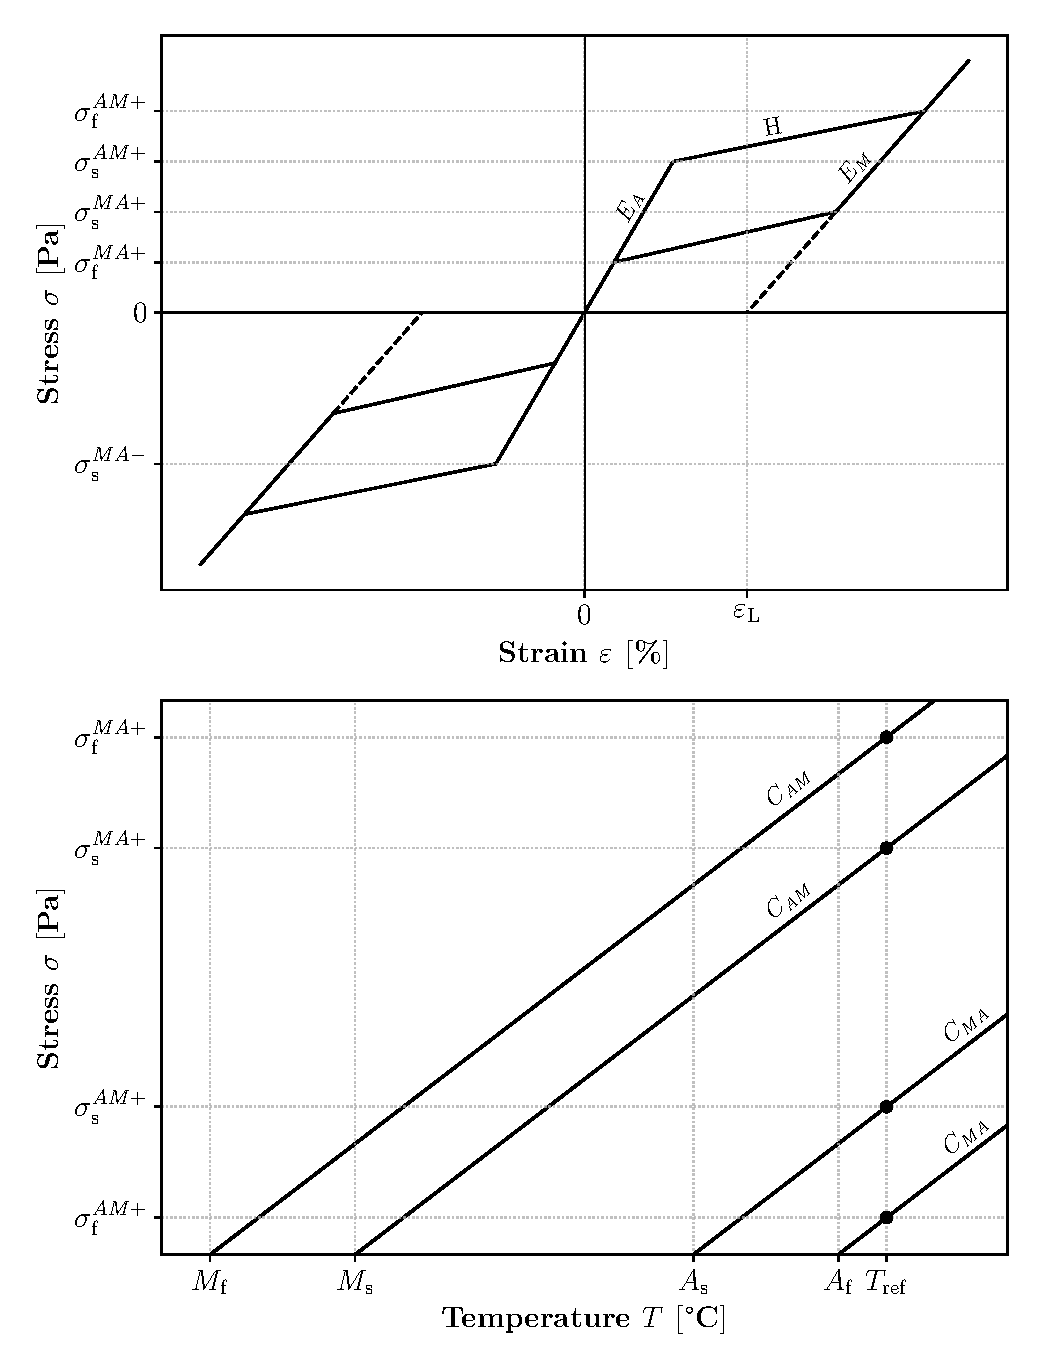
\includegraphics[width=0.75\textwidth]{images/chap2/fem-wp-graph.pdf}
    \caption{A visual representation of the various parameters required to define the Shape Memory Effect within the FEM model based on the work by \cite{jaberAnsysParametersShape2018}.}
    \label{fig:fem-wp-graph}
\end{figure}

\begin{equation}
    \label{eq:fem-h}
    H = \frac{\sigmafamplus-\sigmasamplus}{\frac{\sigmafamplus}{E_M}+\eL-\frac{\sigmasamplus}{E_A}}
\end{equation}

The temperature scaling parameter is defined, as defined in \cref{eq:fem-C}, and is shown in \cref{fig:fem-wp-graph} by the relationship between the transformation temperature and stress.

\begin{equation}
    \label{eq:fem-C}
    C = C^{AM}=C^{MA}=\frac{\sigmafmaplus}{T_\mathrm{ref}-\Af}
\end{equation}

In most constitutive models, the SMA behaves symmetrically in tension and compression. However, numerous experimental tests show that there is an asymmetrical behaviour between the two and in this model, the lode dependency parameter, $\beta$, as defined below, takes into account this asymmetry.

\begin{equation}
    \label{eq:fem-beta}
    \beta = \frac{|\sigmasamminus|-\sigmasamplus}{|\sigmasamminus|+\sigmasamplus}
\end{equation}

Using the FEM simulations of the SMA, complex structures composed of the alloy can be used to predict the behaviour of the SME when the thermal load is applied. This strategy can be used to estimate the force requirements when sizing the biasing elements and the stroke output of the overall actuator when activated. However, the computation time of the simulation can be high and thus, using this strategy to optimize design might not be feasible. Using the one-dimensional analytical models validated by the FEM simulations can be effective in designing SMA actuators.

\section{Stroke Estimation of SMA Actuators}\label{sec:stroke-estimation}
As the biasing element plays a major role in the operation of the SMA actuator, the first step in estimating the stroke and force characteristics of the actuator consists of determining the force-displacement profile of the biasing element. In this section, the biasing element is considered to be a linear spring as this is the most common type of SMA actuator implementation. However, this methodology can be applied to any biasing element as soon as its behaviour has been modelled. With the help of \cref{eq:f-x-sma} and the dimensions of the SMA, such as the cross-section area of the SMA, $A_\mathrm{SMA}$, and the length of the SMA, $L_\mathrm{SMA}$, the stress-strain characteristics of the SMA can be converted into the required force-displacement profile used to compare with the biasing element. In the case of a linear spring with stiffness, $K_\mathrm{BS}$, \cref{eq:bias-spring} can be used to obtain the relevant force-displacement curve of the biasing spring.

\begin{equation}
    \label{eq:f-x-sma}
    F = A_\mathrm{SMA}\sigma,~x = L_\mathrm{SMA}\varepsilon
\end{equation}

\begin{equation}
    \label{eq:bias-spring}
    \sigma A_\mathrm{SMA} = -K_\mathrm{BS}\left(L_\mathrm{SMA}\varepsilon-x_\mathrm{off}\right)
\end{equation}
% SMA - Bias spring diagram with variables
\begin{figure}[hbt]
    \centering
    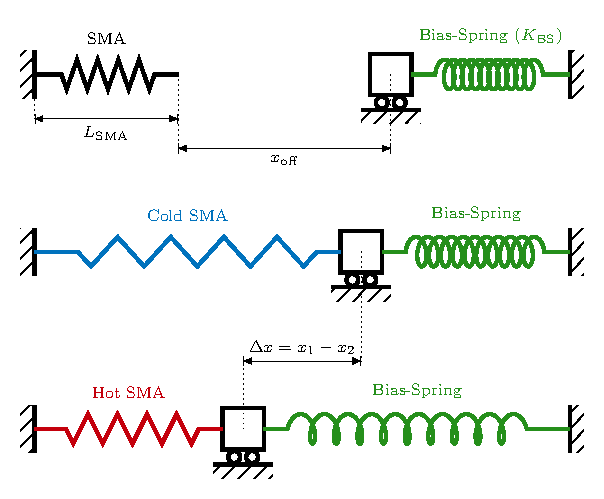
\includegraphics[width=0.66\textwidth]{images/chap2/bias-spring-diagram.pdf}
    \caption{A schematic representation of the Bias-spring SMA actuator showing the different variables and the stroke estimation based on the SMA temperature.}
    \label{fig:bias-spring-diagram}
\end{figure}

In \cref{fig:bias-spring-diagram}, the schematic of a standard bias-spring SMA actuator shown the simplified operation of the actuator. Here, the SMA and the biasing are separated by a distance, $x_\mathrm{off}$, so as to apply the initial prestress to the SMA element. This offset allows the SMA to be biasing and detwinned at the lower temperatures. As shown in the diagram, when heated the SMA contracts to a length, $L_\mathrm{SMA}+x_2$, and when cooled, the SMA elongates to a length, $L_\mathrm{SMA}+x_1$. Thus, the stroke of the actuator, $\Delta x$, can be easily deduce by taking the difference between the two lengths, $x_1-x_2$, as shown in the figure.

% Stroke estimation using spring model
The stroke of the bias-spring SMA actuator can be estimated using the \cite{brinsonOneDimensionalConstitutiveBehavior1993} model. Firstly, with a known temperature, $T < \As$, the martensite fraction can be deduced using \cref{eq:brinson_conv_xis} and \cref{eq:brinson_conv_xit}. When substituting $\sigma$ with the bias-spring equation \ref{eq:bias-spring}, a relationship between $\xi$ and $\varepsilon$ can be obtained. This relationship, combined with \cref{eq:brinson_model_3}, the strain, $\varepsilon$, and consequently, the elongation, $x$, of the SMA can be estimated with respect to its temperature, $T$. In most cases, however, the cold state exists completely within the detwinned state and the hot state exists entirely in the A phase so as to maximise the stroke of the SMA actuator. This consideration can simplify the analytical model.

In the case of the cold state, with $T_1 < \Mf$, $\xi_S=1$ and $\xi_T=0$, the elongation of the cold bias-spring SMA actuator, $x_1$ can be estimated as:
\begin{equation}
    \label{eq:bias-spring-sma-cold-elongation}
    x_1 = \frac{\KBS\xoff-\ASMA(\Omega_S+\Theta(T_1-T_0))}{\frac{\ASMA E_M}{\LSMA}+\KBS}
\end{equation}
Similarly, in the case of the hot state, where the SMA has been completely transformed into the A phase, with $T_2 < \Af$, $\xi=0$, the elongation of the hot bias-spring SMA actuator, $x_2$ can be estimated as:
\begin{equation}
    \label{eq:bias-spring-sma-hot-elongation}
    x_2 = \frac{\KBS\xoff-\ASMA\Theta(T_1-T_0)}{\frac{\ASMA E_A}{\LSMA}+\KBS}
\end{equation}

\begin{figure}[hbt]
    \centering
    \resizebox{0.75\textwidth}{!}{%% Creator: Matplotlib, PGF backend
%%
%% To include the figure in your LaTeX document, write
%%   \input{<filename>.pgf}
%%
%% Make sure the required packages are loaded in your preamble
%%   \usepackage{pgf}
%%
%% and, on pdftex
%%   \usepackage[utf8]{inputenc}\DeclareUnicodeCharacter{2212}{-}
%%
%% or, on luatex and xetex
%%   \usepackage{unicode-math}
%%
%% Figures using additional raster images can only be included by \input if
%% they are in the same directory as the main LaTeX file. For loading figures
%% from other directories you can use the `import` package
%%   \usepackage{import}
%%
%% and then include the figures with
%%   \import{<path to file>}{<filename>.pgf}
%%
%% Matplotlib used the following preamble
%%
\begingroup%
\makeatletter%
\begin{pgfpicture}%
\pgfpathrectangle{\pgfpointorigin}{\pgfqpoint{7.215810in}{4.502126in}}%
\pgfusepath{use as bounding box, clip}%
\begin{pgfscope}%
\pgfsetbuttcap%
\pgfsetmiterjoin%
\pgfsetlinewidth{0.000000pt}%
\definecolor{currentstroke}{rgb}{0.000000,0.000000,0.000000}%
\pgfsetstrokecolor{currentstroke}%
\pgfsetstrokeopacity{0.000000}%
\pgfsetdash{}{0pt}%
\pgfpathmoveto{\pgfqpoint{0.000000in}{0.000000in}}%
\pgfpathlineto{\pgfqpoint{7.215810in}{0.000000in}}%
\pgfpathlineto{\pgfqpoint{7.215810in}{4.502126in}}%
\pgfpathlineto{\pgfqpoint{0.000000in}{4.502126in}}%
\pgfpathclose%
\pgfusepath{}%
\end{pgfscope}%
\begin{pgfscope}%
\pgfsetbuttcap%
\pgfsetmiterjoin%
\pgfsetlinewidth{0.000000pt}%
\definecolor{currentstroke}{rgb}{0.000000,0.000000,0.000000}%
\pgfsetstrokecolor{currentstroke}%
\pgfsetstrokeopacity{0.000000}%
\pgfsetdash{}{0pt}%
\pgfpathmoveto{\pgfqpoint{0.769060in}{0.706126in}}%
\pgfpathlineto{\pgfqpoint{6.969060in}{0.706126in}}%
\pgfpathlineto{\pgfqpoint{6.969060in}{4.402126in}}%
\pgfpathlineto{\pgfqpoint{0.769060in}{4.402126in}}%
\pgfpathclose%
\pgfusepath{}%
\end{pgfscope}%
\begin{pgfscope}%
\pgfpathrectangle{\pgfqpoint{0.769060in}{0.706126in}}{\pgfqpoint{6.200000in}{3.696000in}}%
\pgfusepath{clip}%
\pgfsetbuttcap%
\pgfsetroundjoin%
\pgfsetlinewidth{0.803000pt}%
\definecolor{currentstroke}{rgb}{0.690196,0.690196,0.690196}%
\pgfsetstrokecolor{currentstroke}%
\pgfsetstrokeopacity{0.750000}%
\pgfsetdash{{0.800000pt}{1.320000pt}}{0.000000pt}%
\pgfpathmoveto{\pgfqpoint{0.769060in}{0.706126in}}%
\pgfpathlineto{\pgfqpoint{0.769060in}{4.402126in}}%
\pgfusepath{stroke}%
\end{pgfscope}%
\begin{pgfscope}%
\pgfsetbuttcap%
\pgfsetroundjoin%
\definecolor{currentfill}{rgb}{0.000000,0.000000,0.000000}%
\pgfsetfillcolor{currentfill}%
\pgfsetlinewidth{0.803000pt}%
\definecolor{currentstroke}{rgb}{0.000000,0.000000,0.000000}%
\pgfsetstrokecolor{currentstroke}%
\pgfsetdash{}{0pt}%
\pgfsys@defobject{currentmarker}{\pgfqpoint{0.000000in}{-0.048611in}}{\pgfqpoint{0.000000in}{0.000000in}}{%
\pgfpathmoveto{\pgfqpoint{0.000000in}{0.000000in}}%
\pgfpathlineto{\pgfqpoint{0.000000in}{-0.048611in}}%
\pgfusepath{stroke,fill}%
}%
\begin{pgfscope}%
\pgfsys@transformshift{0.769060in}{0.706126in}%
\pgfsys@useobject{currentmarker}{}%
\end{pgfscope}%
\end{pgfscope}%
\begin{pgfscope}%
\definecolor{textcolor}{rgb}{0.000000,0.000000,0.000000}%
\pgfsetstrokecolor{textcolor}%
\pgfsetfillcolor{textcolor}%
\pgftext[x=0.769060in,y=0.608904in,,top]{\color{textcolor}\rmfamily\fontsize{16.000000}{19.200000}\selectfont 0}%
\end{pgfscope}%
\begin{pgfscope}%
\pgfpathrectangle{\pgfqpoint{0.769060in}{0.706126in}}{\pgfqpoint{6.200000in}{3.696000in}}%
\pgfusepath{clip}%
\pgfsetbuttcap%
\pgfsetroundjoin%
\pgfsetlinewidth{0.803000pt}%
\definecolor{currentstroke}{rgb}{0.690196,0.690196,0.690196}%
\pgfsetstrokecolor{currentstroke}%
\pgfsetstrokeopacity{0.750000}%
\pgfsetdash{{0.800000pt}{1.320000pt}}{0.000000pt}%
\pgfpathmoveto{\pgfqpoint{1.011802in}{0.706126in}}%
\pgfpathlineto{\pgfqpoint{1.011802in}{4.402126in}}%
\pgfusepath{stroke}%
\end{pgfscope}%
\begin{pgfscope}%
\pgfsetbuttcap%
\pgfsetroundjoin%
\definecolor{currentfill}{rgb}{0.000000,0.000000,0.000000}%
\pgfsetfillcolor{currentfill}%
\pgfsetlinewidth{0.803000pt}%
\definecolor{currentstroke}{rgb}{0.000000,0.000000,0.000000}%
\pgfsetstrokecolor{currentstroke}%
\pgfsetdash{}{0pt}%
\pgfsys@defobject{currentmarker}{\pgfqpoint{0.000000in}{-0.048611in}}{\pgfqpoint{0.000000in}{0.000000in}}{%
\pgfpathmoveto{\pgfqpoint{0.000000in}{0.000000in}}%
\pgfpathlineto{\pgfqpoint{0.000000in}{-0.048611in}}%
\pgfusepath{stroke,fill}%
}%
\begin{pgfscope}%
\pgfsys@transformshift{1.011802in}{0.706126in}%
\pgfsys@useobject{currentmarker}{}%
\end{pgfscope}%
\end{pgfscope}%
\begin{pgfscope}%
\definecolor{textcolor}{rgb}{0.000000,0.000000,0.000000}%
\pgfsetstrokecolor{textcolor}%
\pgfsetfillcolor{textcolor}%
\pgftext[x=1.011802in,y=0.608904in,,top]{\color{textcolor}\rmfamily\fontsize{16.000000}{19.200000}\selectfont \(\displaystyle \varepsilon_2\)}%
\end{pgfscope}%
\begin{pgfscope}%
\pgfpathrectangle{\pgfqpoint{0.769060in}{0.706126in}}{\pgfqpoint{6.200000in}{3.696000in}}%
\pgfusepath{clip}%
\pgfsetbuttcap%
\pgfsetroundjoin%
\pgfsetlinewidth{0.803000pt}%
\definecolor{currentstroke}{rgb}{0.690196,0.690196,0.690196}%
\pgfsetstrokecolor{currentstroke}%
\pgfsetstrokeopacity{0.750000}%
\pgfsetdash{{0.800000pt}{1.320000pt}}{0.000000pt}%
\pgfpathmoveto{\pgfqpoint{3.392873in}{0.706126in}}%
\pgfpathlineto{\pgfqpoint{3.392873in}{4.402126in}}%
\pgfusepath{stroke}%
\end{pgfscope}%
\begin{pgfscope}%
\pgfsetbuttcap%
\pgfsetroundjoin%
\definecolor{currentfill}{rgb}{0.000000,0.000000,0.000000}%
\pgfsetfillcolor{currentfill}%
\pgfsetlinewidth{0.803000pt}%
\definecolor{currentstroke}{rgb}{0.000000,0.000000,0.000000}%
\pgfsetstrokecolor{currentstroke}%
\pgfsetdash{}{0pt}%
\pgfsys@defobject{currentmarker}{\pgfqpoint{0.000000in}{-0.048611in}}{\pgfqpoint{0.000000in}{0.000000in}}{%
\pgfpathmoveto{\pgfqpoint{0.000000in}{0.000000in}}%
\pgfpathlineto{\pgfqpoint{0.000000in}{-0.048611in}}%
\pgfusepath{stroke,fill}%
}%
\begin{pgfscope}%
\pgfsys@transformshift{3.392873in}{0.706126in}%
\pgfsys@useobject{currentmarker}{}%
\end{pgfscope}%
\end{pgfscope}%
\begin{pgfscope}%
\definecolor{textcolor}{rgb}{0.000000,0.000000,0.000000}%
\pgfsetstrokecolor{textcolor}%
\pgfsetfillcolor{textcolor}%
\pgftext[x=3.392873in,y=0.608904in,,top]{\color{textcolor}\rmfamily\fontsize{16.000000}{19.200000}\selectfont \(\displaystyle \varepsilon_1\)}%
\end{pgfscope}%
\begin{pgfscope}%
\pgfpathrectangle{\pgfqpoint{0.769060in}{0.706126in}}{\pgfqpoint{6.200000in}{3.696000in}}%
\pgfusepath{clip}%
\pgfsetbuttcap%
\pgfsetroundjoin%
\pgfsetlinewidth{0.803000pt}%
\definecolor{currentstroke}{rgb}{0.690196,0.690196,0.690196}%
\pgfsetstrokecolor{currentstroke}%
\pgfsetstrokeopacity{0.750000}%
\pgfsetdash{{0.800000pt}{1.320000pt}}{0.000000pt}%
\pgfpathmoveto{\pgfqpoint{3.094060in}{0.706126in}}%
\pgfpathlineto{\pgfqpoint{3.094060in}{4.402126in}}%
\pgfusepath{stroke}%
\end{pgfscope}%
\begin{pgfscope}%
\pgfsetbuttcap%
\pgfsetroundjoin%
\definecolor{currentfill}{rgb}{0.000000,0.000000,0.000000}%
\pgfsetfillcolor{currentfill}%
\pgfsetlinewidth{0.803000pt}%
\definecolor{currentstroke}{rgb}{0.000000,0.000000,0.000000}%
\pgfsetstrokecolor{currentstroke}%
\pgfsetdash{}{0pt}%
\pgfsys@defobject{currentmarker}{\pgfqpoint{0.000000in}{-0.048611in}}{\pgfqpoint{0.000000in}{0.000000in}}{%
\pgfpathmoveto{\pgfqpoint{0.000000in}{0.000000in}}%
\pgfpathlineto{\pgfqpoint{0.000000in}{-0.048611in}}%
\pgfusepath{stroke,fill}%
}%
\begin{pgfscope}%
\pgfsys@transformshift{3.094060in}{0.706126in}%
\pgfsys@useobject{currentmarker}{}%
\end{pgfscope}%
\end{pgfscope}%
\begin{pgfscope}%
\definecolor{textcolor}{rgb}{0.000000,0.000000,0.000000}%
\pgfsetstrokecolor{textcolor}%
\pgfsetfillcolor{textcolor}%
\pgftext[x=3.094060in,y=0.608904in,,top]{\color{textcolor}\rmfamily\fontsize{16.000000}{19.200000}\selectfont \(\displaystyle \varepsilon_{\mathrm{L}}\)}%
\end{pgfscope}%
\begin{pgfscope}%
\pgfpathrectangle{\pgfqpoint{0.769060in}{0.706126in}}{\pgfqpoint{6.200000in}{3.696000in}}%
\pgfusepath{clip}%
\pgfsetbuttcap%
\pgfsetroundjoin%
\pgfsetlinewidth{0.803000pt}%
\definecolor{currentstroke}{rgb}{0.690196,0.690196,0.690196}%
\pgfsetstrokecolor{currentstroke}%
\pgfsetstrokeopacity{0.750000}%
\pgfsetdash{{0.800000pt}{1.320000pt}}{0.000000pt}%
\pgfpathmoveto{\pgfqpoint{6.969060in}{0.706126in}}%
\pgfpathlineto{\pgfqpoint{6.969060in}{4.402126in}}%
\pgfusepath{stroke}%
\end{pgfscope}%
\begin{pgfscope}%
\pgfsetbuttcap%
\pgfsetroundjoin%
\definecolor{currentfill}{rgb}{0.000000,0.000000,0.000000}%
\pgfsetfillcolor{currentfill}%
\pgfsetlinewidth{0.803000pt}%
\definecolor{currentstroke}{rgb}{0.000000,0.000000,0.000000}%
\pgfsetstrokecolor{currentstroke}%
\pgfsetdash{}{0pt}%
\pgfsys@defobject{currentmarker}{\pgfqpoint{0.000000in}{-0.048611in}}{\pgfqpoint{0.000000in}{0.000000in}}{%
\pgfpathmoveto{\pgfqpoint{0.000000in}{0.000000in}}%
\pgfpathlineto{\pgfqpoint{0.000000in}{-0.048611in}}%
\pgfusepath{stroke,fill}%
}%
\begin{pgfscope}%
\pgfsys@transformshift{6.969060in}{0.706126in}%
\pgfsys@useobject{currentmarker}{}%
\end{pgfscope}%
\end{pgfscope}%
\begin{pgfscope}%
\definecolor{textcolor}{rgb}{0.000000,0.000000,0.000000}%
\pgfsetstrokecolor{textcolor}%
\pgfsetfillcolor{textcolor}%
\pgftext[x=6.969060in,y=0.608904in,,top]{\color{textcolor}\rmfamily\fontsize{16.000000}{19.200000}\selectfont \(\displaystyle \varepsilon_{\mathrm{off}}\)}%
\end{pgfscope}%
\begin{pgfscope}%
\definecolor{textcolor}{rgb}{0.000000,0.000000,0.000000}%
\pgfsetstrokecolor{textcolor}%
\pgfsetfillcolor{textcolor}%
\pgftext[x=3.869060in,y=0.340000in,,top]{\color{textcolor}\rmfamily\fontsize{16.000000}{19.200000}\bfseries\selectfont Strain \(\displaystyle \varepsilon\) [\%]}%
\end{pgfscope}%
\begin{pgfscope}%
\pgfpathrectangle{\pgfqpoint{0.769060in}{0.706126in}}{\pgfqpoint{6.200000in}{3.696000in}}%
\pgfusepath{clip}%
\pgfsetbuttcap%
\pgfsetroundjoin%
\pgfsetlinewidth{0.803000pt}%
\definecolor{currentstroke}{rgb}{0.690196,0.690196,0.690196}%
\pgfsetstrokecolor{currentstroke}%
\pgfsetstrokeopacity{0.750000}%
\pgfsetdash{{0.800000pt}{1.320000pt}}{0.000000pt}%
\pgfpathmoveto{\pgfqpoint{0.769060in}{0.706126in}}%
\pgfpathlineto{\pgfqpoint{6.969060in}{0.706126in}}%
\pgfusepath{stroke}%
\end{pgfscope}%
\begin{pgfscope}%
\pgfsetbuttcap%
\pgfsetroundjoin%
\definecolor{currentfill}{rgb}{0.000000,0.000000,0.000000}%
\pgfsetfillcolor{currentfill}%
\pgfsetlinewidth{0.803000pt}%
\definecolor{currentstroke}{rgb}{0.000000,0.000000,0.000000}%
\pgfsetstrokecolor{currentstroke}%
\pgfsetdash{}{0pt}%
\pgfsys@defobject{currentmarker}{\pgfqpoint{-0.048611in}{0.000000in}}{\pgfqpoint{-0.000000in}{0.000000in}}{%
\pgfpathmoveto{\pgfqpoint{-0.000000in}{0.000000in}}%
\pgfpathlineto{\pgfqpoint{-0.048611in}{0.000000in}}%
\pgfusepath{stroke,fill}%
}%
\begin{pgfscope}%
\pgfsys@transformshift{0.769060in}{0.706126in}%
\pgfsys@useobject{currentmarker}{}%
\end{pgfscope}%
\end{pgfscope}%
\begin{pgfscope}%
\definecolor{textcolor}{rgb}{0.000000,0.000000,0.000000}%
\pgfsetstrokecolor{textcolor}%
\pgfsetfillcolor{textcolor}%
\pgftext[x=0.561769in, y=0.622793in, left, base]{\color{textcolor}\rmfamily\fontsize{16.000000}{19.200000}\selectfont 0}%
\end{pgfscope}%
\begin{pgfscope}%
\pgfpathrectangle{\pgfqpoint{0.769060in}{0.706126in}}{\pgfqpoint{6.200000in}{3.696000in}}%
\pgfusepath{clip}%
\pgfsetbuttcap%
\pgfsetroundjoin%
\pgfsetlinewidth{0.803000pt}%
\definecolor{currentstroke}{rgb}{0.690196,0.690196,0.690196}%
\pgfsetstrokecolor{currentstroke}%
\pgfsetstrokeopacity{0.750000}%
\pgfsetdash{{0.800000pt}{1.320000pt}}{0.000000pt}%
\pgfpathmoveto{\pgfqpoint{0.769060in}{1.445326in}}%
\pgfpathlineto{\pgfqpoint{6.969060in}{1.445326in}}%
\pgfusepath{stroke}%
\end{pgfscope}%
\begin{pgfscope}%
\pgfsetbuttcap%
\pgfsetroundjoin%
\definecolor{currentfill}{rgb}{0.000000,0.000000,0.000000}%
\pgfsetfillcolor{currentfill}%
\pgfsetlinewidth{0.803000pt}%
\definecolor{currentstroke}{rgb}{0.000000,0.000000,0.000000}%
\pgfsetstrokecolor{currentstroke}%
\pgfsetdash{}{0pt}%
\pgfsys@defobject{currentmarker}{\pgfqpoint{-0.048611in}{0.000000in}}{\pgfqpoint{-0.000000in}{0.000000in}}{%
\pgfpathmoveto{\pgfqpoint{-0.000000in}{0.000000in}}%
\pgfpathlineto{\pgfqpoint{-0.048611in}{0.000000in}}%
\pgfusepath{stroke,fill}%
}%
\begin{pgfscope}%
\pgfsys@transformshift{0.769060in}{1.445326in}%
\pgfsys@useobject{currentmarker}{}%
\end{pgfscope}%
\end{pgfscope}%
\begin{pgfscope}%
\definecolor{textcolor}{rgb}{0.000000,0.000000,0.000000}%
\pgfsetstrokecolor{textcolor}%
\pgfsetfillcolor{textcolor}%
\pgftext[x=0.395555in, y=1.363039in, left, base]{\color{textcolor}\rmfamily\fontsize{16.000000}{19.200000}\selectfont \(\displaystyle \sigma_\mathrm{s}^\mathrm{cr}\)}%
\end{pgfscope}%
\begin{pgfscope}%
\pgfpathrectangle{\pgfqpoint{0.769060in}{0.706126in}}{\pgfqpoint{6.200000in}{3.696000in}}%
\pgfusepath{clip}%
\pgfsetbuttcap%
\pgfsetroundjoin%
\pgfsetlinewidth{0.803000pt}%
\definecolor{currentstroke}{rgb}{0.690196,0.690196,0.690196}%
\pgfsetstrokecolor{currentstroke}%
\pgfsetstrokeopacity{0.750000}%
\pgfsetdash{{0.800000pt}{1.320000pt}}{0.000000pt}%
\pgfpathmoveto{\pgfqpoint{0.769060in}{2.659726in}}%
\pgfpathlineto{\pgfqpoint{6.969060in}{2.659726in}}%
\pgfusepath{stroke}%
\end{pgfscope}%
\begin{pgfscope}%
\pgfsetbuttcap%
\pgfsetroundjoin%
\definecolor{currentfill}{rgb}{0.000000,0.000000,0.000000}%
\pgfsetfillcolor{currentfill}%
\pgfsetlinewidth{0.803000pt}%
\definecolor{currentstroke}{rgb}{0.000000,0.000000,0.000000}%
\pgfsetstrokecolor{currentstroke}%
\pgfsetdash{}{0pt}%
\pgfsys@defobject{currentmarker}{\pgfqpoint{-0.048611in}{0.000000in}}{\pgfqpoint{-0.000000in}{0.000000in}}{%
\pgfpathmoveto{\pgfqpoint{-0.000000in}{0.000000in}}%
\pgfpathlineto{\pgfqpoint{-0.048611in}{0.000000in}}%
\pgfusepath{stroke,fill}%
}%
\begin{pgfscope}%
\pgfsys@transformshift{0.769060in}{2.659726in}%
\pgfsys@useobject{currentmarker}{}%
\end{pgfscope}%
\end{pgfscope}%
\begin{pgfscope}%
\definecolor{textcolor}{rgb}{0.000000,0.000000,0.000000}%
\pgfsetstrokecolor{textcolor}%
\pgfsetfillcolor{textcolor}%
\pgftext[x=0.395555in, y=2.577439in, left, base]{\color{textcolor}\rmfamily\fontsize{16.000000}{19.200000}\selectfont \(\displaystyle \sigma_\mathrm{f}^\mathrm{cr}\)}%
\end{pgfscope}%
\begin{pgfscope}%
\definecolor{textcolor}{rgb}{0.000000,0.000000,0.000000}%
\pgfsetstrokecolor{textcolor}%
\pgfsetfillcolor{textcolor}%
\pgftext[x=0.340000in,y=2.554126in,,bottom,rotate=90.000000]{\color{textcolor}\rmfamily\fontsize{16.000000}{19.200000}\bfseries\selectfont Stress \(\displaystyle \sigma\) [Pa]}%
\end{pgfscope}%
\begin{pgfscope}%
\pgfpathrectangle{\pgfqpoint{0.769060in}{0.706126in}}{\pgfqpoint{6.200000in}{3.696000in}}%
\pgfusepath{clip}%
\pgfsetrectcap%
\pgfsetroundjoin%
\pgfsetlinewidth{1.505625pt}%
\definecolor{currentstroke}{rgb}{0.000000,0.447059,0.741176}%
\pgfsetstrokecolor{currentstroke}%
\pgfsetdash{}{0pt}%
\pgfpathmoveto{\pgfqpoint{0.769060in}{0.706126in}}%
\pgfpathlineto{\pgfqpoint{0.775322in}{0.748793in}}%
\pgfpathlineto{\pgfqpoint{0.781585in}{0.791459in}}%
\pgfpathlineto{\pgfqpoint{0.787848in}{0.834126in}}%
\pgfpathlineto{\pgfqpoint{0.794110in}{0.876793in}}%
\pgfpathlineto{\pgfqpoint{0.800373in}{0.919459in}}%
\pgfpathlineto{\pgfqpoint{0.806635in}{0.962126in}}%
\pgfpathlineto{\pgfqpoint{0.812898in}{1.004793in}}%
\pgfpathlineto{\pgfqpoint{0.819161in}{1.047459in}}%
\pgfpathlineto{\pgfqpoint{0.825423in}{1.090126in}}%
\pgfpathlineto{\pgfqpoint{0.831686in}{1.132793in}}%
\pgfpathlineto{\pgfqpoint{0.837949in}{1.175459in}}%
\pgfpathlineto{\pgfqpoint{0.844211in}{1.218126in}}%
\pgfpathlineto{\pgfqpoint{0.850474in}{1.260793in}}%
\pgfpathlineto{\pgfqpoint{0.856736in}{1.303459in}}%
\pgfpathlineto{\pgfqpoint{0.862999in}{1.346126in}}%
\pgfpathlineto{\pgfqpoint{0.869262in}{1.388793in}}%
\pgfpathlineto{\pgfqpoint{0.875524in}{1.431459in}}%
\pgfpathlineto{\pgfqpoint{0.885012in}{1.474126in}}%
\pgfpathlineto{\pgfqpoint{0.907861in}{1.516793in}}%
\pgfpathlineto{\pgfqpoint{0.944617in}{1.559459in}}%
\pgfpathlineto{\pgfqpoint{0.994909in}{1.602126in}}%
\pgfpathlineto{\pgfqpoint{1.058201in}{1.644793in}}%
\pgfpathlineto{\pgfqpoint{1.133800in}{1.687459in}}%
\pgfpathlineto{\pgfqpoint{1.220861in}{1.730126in}}%
\pgfpathlineto{\pgfqpoint{1.318400in}{1.772793in}}%
\pgfpathlineto{\pgfqpoint{1.425308in}{1.815459in}}%
\pgfpathlineto{\pgfqpoint{1.540359in}{1.858126in}}%
\pgfpathlineto{\pgfqpoint{1.662229in}{1.900793in}}%
\pgfpathlineto{\pgfqpoint{1.789511in}{1.943459in}}%
\pgfpathlineto{\pgfqpoint{1.920732in}{1.986126in}}%
\pgfpathlineto{\pgfqpoint{2.054372in}{2.028793in}}%
\pgfpathlineto{\pgfqpoint{2.188880in}{2.071459in}}%
\pgfpathlineto{\pgfqpoint{2.322695in}{2.114126in}}%
\pgfpathlineto{\pgfqpoint{2.454265in}{2.156793in}}%
\pgfpathlineto{\pgfqpoint{2.582065in}{2.199459in}}%
\pgfpathlineto{\pgfqpoint{2.704615in}{2.242126in}}%
\pgfpathlineto{\pgfqpoint{2.820501in}{2.284793in}}%
\pgfpathlineto{\pgfqpoint{2.928388in}{2.327459in}}%
\pgfpathlineto{\pgfqpoint{3.027039in}{2.370126in}}%
\pgfpathlineto{\pgfqpoint{3.115331in}{2.412793in}}%
\pgfpathlineto{\pgfqpoint{3.192263in}{2.455459in}}%
\pgfpathlineto{\pgfqpoint{3.256978in}{2.498126in}}%
\pgfpathlineto{\pgfqpoint{3.308762in}{2.540793in}}%
\pgfpathlineto{\pgfqpoint{3.347063in}{2.583459in}}%
\pgfpathlineto{\pgfqpoint{3.371489in}{2.626126in}}%
\pgfpathlineto{\pgfqpoint{3.382141in}{2.668793in}}%
\pgfpathlineto{\pgfqpoint{3.388403in}{2.711459in}}%
\pgfpathlineto{\pgfqpoint{3.394666in}{2.754126in}}%
\pgfpathlineto{\pgfqpoint{3.400928in}{2.796793in}}%
\pgfpathlineto{\pgfqpoint{3.407191in}{2.839459in}}%
\pgfpathlineto{\pgfqpoint{3.413454in}{2.882126in}}%
\pgfpathlineto{\pgfqpoint{3.419716in}{2.924793in}}%
\pgfpathlineto{\pgfqpoint{3.425979in}{2.967459in}}%
\pgfpathlineto{\pgfqpoint{3.432242in}{3.010126in}}%
\pgfpathlineto{\pgfqpoint{3.438504in}{3.052793in}}%
\pgfpathlineto{\pgfqpoint{3.444767in}{3.095459in}}%
\pgfpathlineto{\pgfqpoint{3.451029in}{3.138126in}}%
\pgfpathlineto{\pgfqpoint{3.457292in}{3.180793in}}%
\pgfpathlineto{\pgfqpoint{3.463555in}{3.223459in}}%
\pgfpathlineto{\pgfqpoint{3.469817in}{3.266126in}}%
\pgfpathlineto{\pgfqpoint{3.476080in}{3.308793in}}%
\pgfpathlineto{\pgfqpoint{3.482343in}{3.351459in}}%
\pgfpathlineto{\pgfqpoint{3.488605in}{3.394126in}}%
\pgfpathlineto{\pgfqpoint{3.494868in}{3.436793in}}%
\pgfpathlineto{\pgfqpoint{3.501130in}{3.479459in}}%
\pgfpathlineto{\pgfqpoint{3.507393in}{3.522126in}}%
\pgfpathlineto{\pgfqpoint{3.513656in}{3.564793in}}%
\pgfpathlineto{\pgfqpoint{3.519918in}{3.607459in}}%
\pgfpathlineto{\pgfqpoint{3.526181in}{3.650126in}}%
\pgfpathlineto{\pgfqpoint{3.532444in}{3.692793in}}%
\pgfpathlineto{\pgfqpoint{3.538706in}{3.735459in}}%
\pgfpathlineto{\pgfqpoint{3.544969in}{3.778126in}}%
\pgfpathlineto{\pgfqpoint{3.551231in}{3.820793in}}%
\pgfpathlineto{\pgfqpoint{3.557494in}{3.863459in}}%
\pgfpathlineto{\pgfqpoint{3.563757in}{3.906126in}}%
\pgfpathlineto{\pgfqpoint{3.570019in}{3.948793in}}%
\pgfpathlineto{\pgfqpoint{3.576282in}{3.991459in}}%
\pgfpathlineto{\pgfqpoint{3.582545in}{4.034126in}}%
\pgfpathlineto{\pgfqpoint{3.588807in}{4.076793in}}%
\pgfpathlineto{\pgfqpoint{3.595070in}{4.119459in}}%
\pgfpathlineto{\pgfqpoint{3.601332in}{4.162126in}}%
\pgfpathlineto{\pgfqpoint{3.607595in}{4.204793in}}%
\pgfpathlineto{\pgfqpoint{3.613858in}{4.247459in}}%
\pgfpathlineto{\pgfqpoint{3.620120in}{4.290126in}}%
\pgfpathlineto{\pgfqpoint{3.626383in}{4.332793in}}%
\pgfpathlineto{\pgfqpoint{3.632646in}{4.375459in}}%
\pgfpathlineto{\pgfqpoint{3.637049in}{4.405459in}}%
\pgfusepath{stroke}%
\end{pgfscope}%
\begin{pgfscope}%
\pgfpathrectangle{\pgfqpoint{0.769060in}{0.706126in}}{\pgfqpoint{6.200000in}{3.696000in}}%
\pgfusepath{clip}%
\pgfsetrectcap%
\pgfsetroundjoin%
\pgfsetlinewidth{1.505625pt}%
\definecolor{currentstroke}{rgb}{0.905882,0.207843,0.219608}%
\pgfsetstrokecolor{currentstroke}%
\pgfsetdash{}{0pt}%
\pgfpathmoveto{\pgfqpoint{0.765726in}{0.953945in}}%
\pgfpathlineto{\pgfqpoint{0.767463in}{0.976126in}}%
\pgfpathlineto{\pgfqpoint{0.770813in}{1.018926in}}%
\pgfpathlineto{\pgfqpoint{0.774164in}{1.061726in}}%
\pgfpathlineto{\pgfqpoint{0.777514in}{1.104526in}}%
\pgfpathlineto{\pgfqpoint{0.780865in}{1.147326in}}%
\pgfpathlineto{\pgfqpoint{0.784215in}{1.190126in}}%
\pgfpathlineto{\pgfqpoint{0.787566in}{1.232926in}}%
\pgfpathlineto{\pgfqpoint{0.790916in}{1.275726in}}%
\pgfpathlineto{\pgfqpoint{0.794267in}{1.318526in}}%
\pgfpathlineto{\pgfqpoint{0.797617in}{1.361326in}}%
\pgfpathlineto{\pgfqpoint{0.800968in}{1.404126in}}%
\pgfpathlineto{\pgfqpoint{0.804318in}{1.446926in}}%
\pgfpathlineto{\pgfqpoint{0.807669in}{1.489726in}}%
\pgfpathlineto{\pgfqpoint{0.811019in}{1.532526in}}%
\pgfpathlineto{\pgfqpoint{0.814370in}{1.575326in}}%
\pgfpathlineto{\pgfqpoint{0.817720in}{1.618126in}}%
\pgfpathlineto{\pgfqpoint{0.821071in}{1.660926in}}%
\pgfpathlineto{\pgfqpoint{0.824421in}{1.703726in}}%
\pgfpathlineto{\pgfqpoint{0.827772in}{1.746526in}}%
\pgfpathlineto{\pgfqpoint{0.831122in}{1.789326in}}%
\pgfpathlineto{\pgfqpoint{0.834473in}{1.832126in}}%
\pgfpathlineto{\pgfqpoint{0.837823in}{1.874926in}}%
\pgfpathlineto{\pgfqpoint{0.841174in}{1.917726in}}%
\pgfpathlineto{\pgfqpoint{0.844524in}{1.960526in}}%
\pgfpathlineto{\pgfqpoint{0.847875in}{2.003326in}}%
\pgfpathlineto{\pgfqpoint{0.851225in}{2.046126in}}%
\pgfpathlineto{\pgfqpoint{0.854576in}{2.088926in}}%
\pgfpathlineto{\pgfqpoint{0.857926in}{2.131726in}}%
\pgfpathlineto{\pgfqpoint{0.861277in}{2.174526in}}%
\pgfpathlineto{\pgfqpoint{0.864627in}{2.217326in}}%
\pgfpathlineto{\pgfqpoint{0.867978in}{2.260126in}}%
\pgfpathlineto{\pgfqpoint{0.871328in}{2.302926in}}%
\pgfpathlineto{\pgfqpoint{0.874679in}{2.345726in}}%
\pgfpathlineto{\pgfqpoint{0.878029in}{2.388526in}}%
\pgfpathlineto{\pgfqpoint{0.881380in}{2.431326in}}%
\pgfpathlineto{\pgfqpoint{0.884730in}{2.474126in}}%
\pgfpathlineto{\pgfqpoint{0.888081in}{2.516926in}}%
\pgfpathlineto{\pgfqpoint{0.891431in}{2.559726in}}%
\pgfpathlineto{\pgfqpoint{0.894782in}{2.602526in}}%
\pgfpathlineto{\pgfqpoint{0.898132in}{2.645326in}}%
\pgfpathlineto{\pgfqpoint{0.901483in}{2.688126in}}%
\pgfpathlineto{\pgfqpoint{0.904833in}{2.730926in}}%
\pgfpathlineto{\pgfqpoint{0.908184in}{2.773726in}}%
\pgfpathlineto{\pgfqpoint{0.911534in}{2.816526in}}%
\pgfpathlineto{\pgfqpoint{0.914885in}{2.859326in}}%
\pgfpathlineto{\pgfqpoint{0.918235in}{2.902126in}}%
\pgfpathlineto{\pgfqpoint{0.921586in}{2.944926in}}%
\pgfpathlineto{\pgfqpoint{0.924936in}{2.987726in}}%
\pgfpathlineto{\pgfqpoint{0.928287in}{3.030526in}}%
\pgfpathlineto{\pgfqpoint{0.931638in}{3.073326in}}%
\pgfpathlineto{\pgfqpoint{0.934988in}{3.116126in}}%
\pgfpathlineto{\pgfqpoint{0.938339in}{3.158926in}}%
\pgfpathlineto{\pgfqpoint{0.941689in}{3.201726in}}%
\pgfpathlineto{\pgfqpoint{0.945040in}{3.244526in}}%
\pgfpathlineto{\pgfqpoint{0.948390in}{3.287326in}}%
\pgfpathlineto{\pgfqpoint{0.951741in}{3.330126in}}%
\pgfpathlineto{\pgfqpoint{0.955091in}{3.372926in}}%
\pgfpathlineto{\pgfqpoint{0.958442in}{3.415726in}}%
\pgfpathlineto{\pgfqpoint{0.961792in}{3.458526in}}%
\pgfpathlineto{\pgfqpoint{0.965143in}{3.501326in}}%
\pgfpathlineto{\pgfqpoint{0.968493in}{3.544126in}}%
\pgfpathlineto{\pgfqpoint{0.971844in}{3.586926in}}%
\pgfpathlineto{\pgfqpoint{0.975194in}{3.629726in}}%
\pgfpathlineto{\pgfqpoint{0.978545in}{3.672526in}}%
\pgfpathlineto{\pgfqpoint{0.981895in}{3.715326in}}%
\pgfpathlineto{\pgfqpoint{0.985246in}{3.758126in}}%
\pgfpathlineto{\pgfqpoint{0.988596in}{3.800926in}}%
\pgfpathlineto{\pgfqpoint{0.991947in}{3.843726in}}%
\pgfpathlineto{\pgfqpoint{0.995297in}{3.886526in}}%
\pgfpathlineto{\pgfqpoint{0.998648in}{3.929326in}}%
\pgfpathlineto{\pgfqpoint{1.001998in}{3.972126in}}%
\pgfpathlineto{\pgfqpoint{1.005349in}{4.014926in}}%
\pgfpathlineto{\pgfqpoint{1.008699in}{4.057726in}}%
\pgfpathlineto{\pgfqpoint{1.012050in}{4.100526in}}%
\pgfpathlineto{\pgfqpoint{1.015400in}{4.143326in}}%
\pgfpathlineto{\pgfqpoint{1.018751in}{4.186126in}}%
\pgfpathlineto{\pgfqpoint{1.022101in}{4.228926in}}%
\pgfpathlineto{\pgfqpoint{1.025452in}{4.271726in}}%
\pgfpathlineto{\pgfqpoint{1.028802in}{4.314526in}}%
\pgfpathlineto{\pgfqpoint{1.032153in}{4.357326in}}%
\pgfpathlineto{\pgfqpoint{1.035503in}{4.400126in}}%
\pgfpathlineto{\pgfqpoint{1.035921in}{4.405459in}}%
\pgfusepath{stroke}%
\end{pgfscope}%
\begin{pgfscope}%
\pgfpathrectangle{\pgfqpoint{0.769060in}{0.706126in}}{\pgfqpoint{6.200000in}{3.696000in}}%
\pgfusepath{clip}%
\pgfsetrectcap%
\pgfsetroundjoin%
\pgfsetlinewidth{1.505625pt}%
\definecolor{currentstroke}{rgb}{0.317647,0.596078,0.423529}%
\pgfsetstrokecolor{currentstroke}%
\pgfsetdash{}{0pt}%
\pgfpathmoveto{\pgfqpoint{0.769060in}{4.235546in}}%
\pgfpathlineto{\pgfqpoint{0.831686in}{4.199895in}}%
\pgfpathlineto{\pgfqpoint{0.894312in}{4.164245in}}%
\pgfpathlineto{\pgfqpoint{0.956939in}{4.128594in}}%
\pgfpathlineto{\pgfqpoint{1.019565in}{4.092943in}}%
\pgfpathlineto{\pgfqpoint{1.082191in}{4.057293in}}%
\pgfpathlineto{\pgfqpoint{1.144817in}{4.021642in}}%
\pgfpathlineto{\pgfqpoint{1.207444in}{3.985991in}}%
\pgfpathlineto{\pgfqpoint{1.270070in}{3.950340in}}%
\pgfpathlineto{\pgfqpoint{1.332696in}{3.914690in}}%
\pgfpathlineto{\pgfqpoint{1.395322in}{3.879039in}}%
\pgfpathlineto{\pgfqpoint{1.457949in}{3.843388in}}%
\pgfpathlineto{\pgfqpoint{1.520575in}{3.807738in}}%
\pgfpathlineto{\pgfqpoint{1.583201in}{3.772087in}}%
\pgfpathlineto{\pgfqpoint{1.645827in}{3.736436in}}%
\pgfpathlineto{\pgfqpoint{1.708454in}{3.700786in}}%
\pgfpathlineto{\pgfqpoint{1.771080in}{3.665135in}}%
\pgfpathlineto{\pgfqpoint{1.833706in}{3.629484in}}%
\pgfpathlineto{\pgfqpoint{1.896332in}{3.593833in}}%
\pgfpathlineto{\pgfqpoint{1.958959in}{3.558183in}}%
\pgfpathlineto{\pgfqpoint{2.021585in}{3.522532in}}%
\pgfpathlineto{\pgfqpoint{2.084211in}{3.486881in}}%
\pgfpathlineto{\pgfqpoint{2.146838in}{3.451231in}}%
\pgfpathlineto{\pgfqpoint{2.209464in}{3.415580in}}%
\pgfpathlineto{\pgfqpoint{2.272090in}{3.379929in}}%
\pgfpathlineto{\pgfqpoint{2.334716in}{3.344278in}}%
\pgfpathlineto{\pgfqpoint{2.397343in}{3.308628in}}%
\pgfpathlineto{\pgfqpoint{2.459969in}{3.272977in}}%
\pgfpathlineto{\pgfqpoint{2.522595in}{3.237326in}}%
\pgfpathlineto{\pgfqpoint{2.585221in}{3.201676in}}%
\pgfpathlineto{\pgfqpoint{2.647848in}{3.166025in}}%
\pgfpathlineto{\pgfqpoint{2.710474in}{3.130374in}}%
\pgfpathlineto{\pgfqpoint{2.773100in}{3.094723in}}%
\pgfpathlineto{\pgfqpoint{2.835726in}{3.059073in}}%
\pgfpathlineto{\pgfqpoint{2.898353in}{3.023422in}}%
\pgfpathlineto{\pgfqpoint{2.960979in}{2.987771in}}%
\pgfpathlineto{\pgfqpoint{3.023605in}{2.952121in}}%
\pgfpathlineto{\pgfqpoint{3.086231in}{2.916470in}}%
\pgfpathlineto{\pgfqpoint{3.148858in}{2.880819in}}%
\pgfpathlineto{\pgfqpoint{3.211484in}{2.845169in}}%
\pgfpathlineto{\pgfqpoint{3.274110in}{2.809518in}}%
\pgfpathlineto{\pgfqpoint{3.336736in}{2.773867in}}%
\pgfpathlineto{\pgfqpoint{3.399363in}{2.738216in}}%
\pgfpathlineto{\pgfqpoint{3.461989in}{2.702566in}}%
\pgfpathlineto{\pgfqpoint{3.524615in}{2.666915in}}%
\pgfpathlineto{\pgfqpoint{3.587242in}{2.631264in}}%
\pgfpathlineto{\pgfqpoint{3.649868in}{2.595614in}}%
\pgfpathlineto{\pgfqpoint{3.712494in}{2.559963in}}%
\pgfpathlineto{\pgfqpoint{3.775120in}{2.524312in}}%
\pgfpathlineto{\pgfqpoint{3.837747in}{2.488661in}}%
\pgfpathlineto{\pgfqpoint{3.900373in}{2.453011in}}%
\pgfpathlineto{\pgfqpoint{3.962999in}{2.417360in}}%
\pgfpathlineto{\pgfqpoint{4.025625in}{2.381709in}}%
\pgfpathlineto{\pgfqpoint{4.088252in}{2.346059in}}%
\pgfpathlineto{\pgfqpoint{4.150878in}{2.310408in}}%
\pgfpathlineto{\pgfqpoint{4.213504in}{2.274757in}}%
\pgfpathlineto{\pgfqpoint{4.276130in}{2.239107in}}%
\pgfpathlineto{\pgfqpoint{4.338757in}{2.203456in}}%
\pgfpathlineto{\pgfqpoint{4.401383in}{2.167805in}}%
\pgfpathlineto{\pgfqpoint{4.464009in}{2.132154in}}%
\pgfpathlineto{\pgfqpoint{4.526635in}{2.096504in}}%
\pgfpathlineto{\pgfqpoint{4.589262in}{2.060853in}}%
\pgfpathlineto{\pgfqpoint{4.651888in}{2.025202in}}%
\pgfpathlineto{\pgfqpoint{4.714514in}{1.989552in}}%
\pgfpathlineto{\pgfqpoint{4.777141in}{1.953901in}}%
\pgfpathlineto{\pgfqpoint{4.839767in}{1.918250in}}%
\pgfpathlineto{\pgfqpoint{4.902393in}{1.882599in}}%
\pgfpathlineto{\pgfqpoint{4.965019in}{1.846949in}}%
\pgfpathlineto{\pgfqpoint{5.027646in}{1.811298in}}%
\pgfpathlineto{\pgfqpoint{5.090272in}{1.775647in}}%
\pgfpathlineto{\pgfqpoint{5.152898in}{1.739997in}}%
\pgfpathlineto{\pgfqpoint{5.215524in}{1.704346in}}%
\pgfpathlineto{\pgfqpoint{5.278151in}{1.668695in}}%
\pgfpathlineto{\pgfqpoint{5.340777in}{1.633044in}}%
\pgfpathlineto{\pgfqpoint{5.403403in}{1.597394in}}%
\pgfpathlineto{\pgfqpoint{5.466029in}{1.561743in}}%
\pgfpathlineto{\pgfqpoint{5.528656in}{1.526092in}}%
\pgfpathlineto{\pgfqpoint{5.591282in}{1.490442in}}%
\pgfpathlineto{\pgfqpoint{5.653908in}{1.454791in}}%
\pgfpathlineto{\pgfqpoint{5.716534in}{1.419140in}}%
\pgfpathlineto{\pgfqpoint{5.779161in}{1.383490in}}%
\pgfpathlineto{\pgfqpoint{5.841787in}{1.347839in}}%
\pgfpathlineto{\pgfqpoint{5.904413in}{1.312188in}}%
\pgfpathlineto{\pgfqpoint{5.967040in}{1.276537in}}%
\pgfpathlineto{\pgfqpoint{6.029666in}{1.240887in}}%
\pgfpathlineto{\pgfqpoint{6.092292in}{1.205236in}}%
\pgfpathlineto{\pgfqpoint{6.154918in}{1.169585in}}%
\pgfpathlineto{\pgfqpoint{6.217545in}{1.133935in}}%
\pgfpathlineto{\pgfqpoint{6.280171in}{1.098284in}}%
\pgfpathlineto{\pgfqpoint{6.342797in}{1.062633in}}%
\pgfpathlineto{\pgfqpoint{6.405423in}{1.026982in}}%
\pgfpathlineto{\pgfqpoint{6.468050in}{0.991332in}}%
\pgfpathlineto{\pgfqpoint{6.530676in}{0.955681in}}%
\pgfpathlineto{\pgfqpoint{6.593302in}{0.920030in}}%
\pgfpathlineto{\pgfqpoint{6.655928in}{0.884380in}}%
\pgfpathlineto{\pgfqpoint{6.718555in}{0.848729in}}%
\pgfpathlineto{\pgfqpoint{6.781181in}{0.813078in}}%
\pgfpathlineto{\pgfqpoint{6.843807in}{0.777428in}}%
\pgfpathlineto{\pgfqpoint{6.906433in}{0.741777in}}%
\pgfpathlineto{\pgfqpoint{6.969060in}{0.706126in}}%
\pgfusepath{stroke}%
\end{pgfscope}%
\begin{pgfscope}%
\pgfpathrectangle{\pgfqpoint{0.769060in}{0.706126in}}{\pgfqpoint{6.200000in}{3.696000in}}%
\pgfusepath{clip}%
\pgfsetbuttcap%
\pgfsetroundjoin%
\definecolor{currentfill}{rgb}{0.000000,0.000000,0.000000}%
\pgfsetfillcolor{currentfill}%
\pgfsetlinewidth{1.003750pt}%
\definecolor{currentstroke}{rgb}{0.000000,0.000000,0.000000}%
\pgfsetstrokecolor{currentstroke}%
\pgfsetdash{}{0pt}%
\pgfsys@defobject{currentmarker}{\pgfqpoint{-0.041667in}{-0.041667in}}{\pgfqpoint{0.041667in}{0.041667in}}{%
\pgfpathmoveto{\pgfqpoint{0.000000in}{-0.041667in}}%
\pgfpathcurveto{\pgfqpoint{0.011050in}{-0.041667in}}{\pgfqpoint{0.021649in}{-0.037276in}}{\pgfqpoint{0.029463in}{-0.029463in}}%
\pgfpathcurveto{\pgfqpoint{0.037276in}{-0.021649in}}{\pgfqpoint{0.041667in}{-0.011050in}}{\pgfqpoint{0.041667in}{0.000000in}}%
\pgfpathcurveto{\pgfqpoint{0.041667in}{0.011050in}}{\pgfqpoint{0.037276in}{0.021649in}}{\pgfqpoint{0.029463in}{0.029463in}}%
\pgfpathcurveto{\pgfqpoint{0.021649in}{0.037276in}}{\pgfqpoint{0.011050in}{0.041667in}}{\pgfqpoint{0.000000in}{0.041667in}}%
\pgfpathcurveto{\pgfqpoint{-0.011050in}{0.041667in}}{\pgfqpoint{-0.021649in}{0.037276in}}{\pgfqpoint{-0.029463in}{0.029463in}}%
\pgfpathcurveto{\pgfqpoint{-0.037276in}{0.021649in}}{\pgfqpoint{-0.041667in}{0.011050in}}{\pgfqpoint{-0.041667in}{0.000000in}}%
\pgfpathcurveto{\pgfqpoint{-0.041667in}{-0.011050in}}{\pgfqpoint{-0.037276in}{-0.021649in}}{\pgfqpoint{-0.029463in}{-0.029463in}}%
\pgfpathcurveto{\pgfqpoint{-0.021649in}{-0.037276in}}{\pgfqpoint{-0.011050in}{-0.041667in}}{\pgfqpoint{0.000000in}{-0.041667in}}%
\pgfpathclose%
\pgfusepath{stroke,fill}%
}%
\begin{pgfscope}%
\pgfsys@transformshift{3.392873in}{2.741911in}%
\pgfsys@useobject{currentmarker}{}%
\end{pgfscope}%
\end{pgfscope}%
\begin{pgfscope}%
\pgfpathrectangle{\pgfqpoint{0.769060in}{0.706126in}}{\pgfqpoint{6.200000in}{3.696000in}}%
\pgfusepath{clip}%
\pgfsetbuttcap%
\pgfsetroundjoin%
\definecolor{currentfill}{rgb}{0.000000,0.000000,0.000000}%
\pgfsetfillcolor{currentfill}%
\pgfsetlinewidth{1.003750pt}%
\definecolor{currentstroke}{rgb}{0.000000,0.000000,0.000000}%
\pgfsetstrokecolor{currentstroke}%
\pgfsetdash{}{0pt}%
\pgfsys@defobject{currentmarker}{\pgfqpoint{-0.041667in}{-0.041667in}}{\pgfqpoint{0.041667in}{0.041667in}}{%
\pgfpathmoveto{\pgfqpoint{0.000000in}{-0.041667in}}%
\pgfpathcurveto{\pgfqpoint{0.011050in}{-0.041667in}}{\pgfqpoint{0.021649in}{-0.037276in}}{\pgfqpoint{0.029463in}{-0.029463in}}%
\pgfpathcurveto{\pgfqpoint{0.037276in}{-0.021649in}}{\pgfqpoint{0.041667in}{-0.011050in}}{\pgfqpoint{0.041667in}{0.000000in}}%
\pgfpathcurveto{\pgfqpoint{0.041667in}{0.011050in}}{\pgfqpoint{0.037276in}{0.021649in}}{\pgfqpoint{0.029463in}{0.029463in}}%
\pgfpathcurveto{\pgfqpoint{0.021649in}{0.037276in}}{\pgfqpoint{0.011050in}{0.041667in}}{\pgfqpoint{0.000000in}{0.041667in}}%
\pgfpathcurveto{\pgfqpoint{-0.011050in}{0.041667in}}{\pgfqpoint{-0.021649in}{0.037276in}}{\pgfqpoint{-0.029463in}{0.029463in}}%
\pgfpathcurveto{\pgfqpoint{-0.037276in}{0.021649in}}{\pgfqpoint{-0.041667in}{0.011050in}}{\pgfqpoint{-0.041667in}{0.000000in}}%
\pgfpathcurveto{\pgfqpoint{-0.041667in}{-0.011050in}}{\pgfqpoint{-0.037276in}{-0.021649in}}{\pgfqpoint{-0.029463in}{-0.029463in}}%
\pgfpathcurveto{\pgfqpoint{-0.021649in}{-0.037276in}}{\pgfqpoint{-0.011050in}{-0.041667in}}{\pgfqpoint{0.000000in}{-0.041667in}}%
\pgfpathclose%
\pgfusepath{stroke,fill}%
}%
\begin{pgfscope}%
\pgfsys@transformshift{1.011802in}{4.097362in}%
\pgfsys@useobject{currentmarker}{}%
\end{pgfscope}%
\end{pgfscope}%
\begin{pgfscope}%
\pgfsetrectcap%
\pgfsetmiterjoin%
\pgfsetlinewidth{0.803000pt}%
\definecolor{currentstroke}{rgb}{0.000000,0.000000,0.000000}%
\pgfsetstrokecolor{currentstroke}%
\pgfsetdash{}{0pt}%
\pgfpathmoveto{\pgfqpoint{0.769060in}{0.706126in}}%
\pgfpathlineto{\pgfqpoint{0.769060in}{4.402126in}}%
\pgfusepath{stroke}%
\end{pgfscope}%
\begin{pgfscope}%
\pgfsetrectcap%
\pgfsetmiterjoin%
\pgfsetlinewidth{0.803000pt}%
\definecolor{currentstroke}{rgb}{0.000000,0.000000,0.000000}%
\pgfsetstrokecolor{currentstroke}%
\pgfsetdash{}{0pt}%
\pgfpathmoveto{\pgfqpoint{6.969060in}{0.706126in}}%
\pgfpathlineto{\pgfqpoint{6.969060in}{4.402126in}}%
\pgfusepath{stroke}%
\end{pgfscope}%
\begin{pgfscope}%
\pgfsetrectcap%
\pgfsetmiterjoin%
\pgfsetlinewidth{0.803000pt}%
\definecolor{currentstroke}{rgb}{0.000000,0.000000,0.000000}%
\pgfsetstrokecolor{currentstroke}%
\pgfsetdash{}{0pt}%
\pgfpathmoveto{\pgfqpoint{0.769060in}{0.706126in}}%
\pgfpathlineto{\pgfqpoint{6.969060in}{0.706126in}}%
\pgfusepath{stroke}%
\end{pgfscope}%
\begin{pgfscope}%
\pgfsetrectcap%
\pgfsetmiterjoin%
\pgfsetlinewidth{0.803000pt}%
\definecolor{currentstroke}{rgb}{0.000000,0.000000,0.000000}%
\pgfsetstrokecolor{currentstroke}%
\pgfsetdash{}{0pt}%
\pgfpathmoveto{\pgfqpoint{0.769060in}{4.402126in}}%
\pgfpathlineto{\pgfqpoint{6.969060in}{4.402126in}}%
\pgfusepath{stroke}%
\end{pgfscope}%
\begin{pgfscope}%
\pgfsetbuttcap%
\pgfsetmiterjoin%
\definecolor{currentfill}{rgb}{1.000000,1.000000,1.000000}%
\pgfsetfillcolor{currentfill}%
\pgfsetfillopacity{0.800000}%
\pgfsetlinewidth{1.003750pt}%
\definecolor{currentstroke}{rgb}{0.800000,0.800000,0.800000}%
\pgfsetstrokecolor{currentstroke}%
\pgfsetstrokeopacity{0.800000}%
\pgfsetdash{}{0pt}%
\pgfpathmoveto{\pgfqpoint{3.126322in}{3.224735in}}%
\pgfpathlineto{\pgfqpoint{6.813504in}{3.224735in}}%
\pgfpathquadraticcurveto{\pgfqpoint{6.857949in}{3.224735in}}{\pgfqpoint{6.857949in}{3.269179in}}%
\pgfpathlineto{\pgfqpoint{6.857949in}{4.246571in}}%
\pgfpathquadraticcurveto{\pgfqpoint{6.857949in}{4.291015in}}{\pgfqpoint{6.813504in}{4.291015in}}%
\pgfpathlineto{\pgfqpoint{3.126322in}{4.291015in}}%
\pgfpathquadraticcurveto{\pgfqpoint{3.081878in}{4.291015in}}{\pgfqpoint{3.081878in}{4.246571in}}%
\pgfpathlineto{\pgfqpoint{3.081878in}{3.269179in}}%
\pgfpathquadraticcurveto{\pgfqpoint{3.081878in}{3.224735in}}{\pgfqpoint{3.126322in}{3.224735in}}%
\pgfpathclose%
\pgfusepath{stroke,fill}%
\end{pgfscope}%
\begin{pgfscope}%
\pgfsetrectcap%
\pgfsetroundjoin%
\pgfsetlinewidth{1.505625pt}%
\definecolor{currentstroke}{rgb}{0.000000,0.447059,0.741176}%
\pgfsetstrokecolor{currentstroke}%
\pgfsetdash{}{0pt}%
\pgfpathmoveto{\pgfqpoint{3.170767in}{4.113237in}}%
\pgfpathlineto{\pgfqpoint{3.615211in}{4.113237in}}%
\pgfusepath{stroke}%
\end{pgfscope}%
\begin{pgfscope}%
\definecolor{textcolor}{rgb}{0.000000,0.000000,0.000000}%
\pgfsetstrokecolor{textcolor}%
\pgfsetfillcolor{textcolor}%
\pgftext[x=3.792989in,y=4.035459in,left,base]{\color{textcolor}\rmfamily\fontsize{16.000000}{19.200000}\selectfont SMA at \(\displaystyle 20 ^{\circ}C\)}%
\end{pgfscope}%
\begin{pgfscope}%
\pgfsetrectcap%
\pgfsetroundjoin%
\pgfsetlinewidth{1.505625pt}%
\definecolor{currentstroke}{rgb}{0.905882,0.207843,0.219608}%
\pgfsetstrokecolor{currentstroke}%
\pgfsetdash{}{0pt}%
\pgfpathmoveto{\pgfqpoint{3.170767in}{3.788778in}}%
\pgfpathlineto{\pgfqpoint{3.615211in}{3.788778in}}%
\pgfusepath{stroke}%
\end{pgfscope}%
\begin{pgfscope}%
\definecolor{textcolor}{rgb}{0.000000,0.000000,0.000000}%
\pgfsetstrokecolor{textcolor}%
\pgfsetfillcolor{textcolor}%
\pgftext[x=3.792989in,y=3.711000in,left,base]{\color{textcolor}\rmfamily\fontsize{16.000000}{19.200000}\selectfont SMA at \(\displaystyle 120 ^{\circ}C\)}%
\end{pgfscope}%
\begin{pgfscope}%
\pgfsetrectcap%
\pgfsetroundjoin%
\pgfsetlinewidth{1.505625pt}%
\definecolor{currentstroke}{rgb}{0.317647,0.596078,0.423529}%
\pgfsetstrokecolor{currentstroke}%
\pgfsetdash{}{0pt}%
\pgfpathmoveto{\pgfqpoint{3.170767in}{3.451201in}}%
\pgfpathlineto{\pgfqpoint{3.615211in}{3.451201in}}%
\pgfusepath{stroke}%
\end{pgfscope}%
\begin{pgfscope}%
\definecolor{textcolor}{rgb}{0.000000,0.000000,0.000000}%
\pgfsetstrokecolor{textcolor}%
\pgfsetfillcolor{textcolor}%
\pgftext[x=3.792989in,y=3.373423in,left,base]{\color{textcolor}\rmfamily\fontsize{16.000000}{19.200000}\selectfont Bias-Spring: \(\displaystyle K_\mathrm{BS} = 3.5\) N/mm}%
\end{pgfscope}%
\end{pgfpicture}%
\makeatother%
\endgroup%
}
    \caption{A plot showing the stroke estimation of a 100 $\mu$m SMA wire actuator using the equations adapted from the \cite{brinsonOneDimensionalConstitutiveBehavior1993} analytical model. Here, the bias spring is offset from the SMA with a distance of $6$ mm and where $\varepsilon_i = x_i / \LSMA$ }
    \label{fig:brinson-sma-spring}
\end{figure}

Thus, as stated previously, the stroke of the system can be deduced as $\Delta x = x_1-x_2$ as shown in \cref{fig:brinson-sma-spring}. This graph shows the sizing of an SMA actuator comprised of a 100 $\mu$m SMA wire of length 30 mm and a biasing spring with a spring constant of 3.5 N/mm separated by a distance of 6 mm. As presented in the previous equations, the Brinson model has been adapted such that the operating points of the actuator and the stroke can be easily estimated. The required forces can be easily obtained by using the spring model described in \cref{eq:bias-spring}. This one-dimensional model can be quite effective when sizing actuators powered by sheets or wires. However, when designing designing actuator with more complex biasing elements or additional mechanical stages, the analytical models of the system can become quite complicated.

\begin{table}[hbt]
    \centering
    \caption{Some examples of the material properties used in the analytical modelling of the SMA actuator.}
    \label{tab:brinson-material-properties}
    % !TEX root = ../../sethomas_thesis_main.tex
\documentclass[border=1mm,
               class=article
               preview]{standalone}

\begin{document}
\renewcommand{\arraystretch}{1.5}
 {\rowcolors{1}{black!5}{black!10}
\begin{tabular}{lcl}
% \begin{tabular}{p{0.45\textwidth-2\tabcolsep}
%                 P{0.1\textwidth-2\tabcolsep}
%                 p{0.15\textwidth-2\tabcolsep}}
   \rowcolor{black} \textbf{\color{white} Material Property} & & \textbf{\color{white} Value}\\
   Martensite Start Temperature & $\Ms$       & 80 $^\circ$C\\
   Martensite Finish Temperature & $\Mf$       & 75 $^\circ$C\\
   Austenite Start Temperature & $\As$       & 85 $^\circ$C\\
   Austenite Finish Temperature & $\Af$       & 90 $^\circ$C\\
   Martensitic Young's Modulus & $E_M$       & 30 GPa\\
   Austenitic Young's Modulus & $E_A$       & 75 GPa\\
   Temperature Scaling Parameter & $C_M,~C_A$ & 10.3 MPa/$^\circ$C\\
   Thermoelastic Constant & $\Theta$ & 0.55 MPa\\
   Maximum Recoverable Strain & $\eL$ & 7.5\% \\
   Detwinning Critical Start Stress & $\sigmacrf$ & 140 MPa\\
   Detwinning Critical Finish Stress & $\sigmacrs$ & 370 MPa\\
\end{tabular}}
\renewcommand{\arraystretch}{1}
\end{document}

\end{table}
% \subsection{Thermal Model}
\section{Simplifying the Sizing of the SMA Actuator}\label{sec:simplified-sma-model}
Owing to their high power densities, SMA-based actuators are extensively used in for mini- and micro-actuation when compared to traditional actuators. However, when considered for applications where high-output forces and strokes are required, they are limited. When under tension in the form of SMA wires, this alloy can generate high forces but can only exert it for up to 8\% of their length. Thus, in many cases where higher strokes are required, these SMA wires are wound into helical springs which allows them to have high strokes but comes at the cost of their output forces.

\begin{figure}[hbt]
    \centering
    \resizebox{0.75\textwidth}{!}{%% Creator: Matplotlib, PGF backend
%%
%% To include the figure in your LaTeX document, write
%%   \input{<filename>.pgf}
%%
%% Make sure the required packages are loaded in your preamble
%%   \usepackage{pgf}
%%
%% and, on pdftex
%%   \usepackage[utf8]{inputenc}\DeclareUnicodeCharacter{2212}{-}
%%
%% or, on luatex and xetex
%%   \usepackage{unicode-math}
%%
%% Figures using additional raster images can only be included by \input if
%% they are in the same directory as the main LaTeX file. For loading figures
%% from other directories you can use the `import` package
%%   \usepackage{import}
%%
%% and then include the figures with
%%   \import{<path to file>}{<filename>.pgf}
%%
%% Matplotlib used the following preamble
%%
\begingroup%
\makeatletter%
\begin{pgfpicture}%
\pgfpathrectangle{\pgfpointorigin}{\pgfqpoint{8.142846in}{4.532178in}}%
\pgfusepath{use as bounding box, clip}%
\begin{pgfscope}%
\pgfsetbuttcap%
\pgfsetmiterjoin%
\pgfsetlinewidth{0.000000pt}%
\definecolor{currentstroke}{rgb}{0.000000,0.000000,0.000000}%
\pgfsetstrokecolor{currentstroke}%
\pgfsetstrokeopacity{0.000000}%
\pgfsetdash{}{0pt}%
\pgfpathmoveto{\pgfqpoint{0.000000in}{0.000000in}}%
\pgfpathlineto{\pgfqpoint{8.142846in}{0.000000in}}%
\pgfpathlineto{\pgfqpoint{8.142846in}{4.532178in}}%
\pgfpathlineto{\pgfqpoint{0.000000in}{4.532178in}}%
\pgfpathclose%
\pgfusepath{}%
\end{pgfscope}%
\begin{pgfscope}%
\pgfsetbuttcap%
\pgfsetmiterjoin%
\pgfsetlinewidth{0.000000pt}%
\definecolor{currentstroke}{rgb}{0.000000,0.000000,0.000000}%
\pgfsetstrokecolor{currentstroke}%
\pgfsetstrokeopacity{0.000000}%
\pgfsetdash{}{0pt}%
\pgfpathmoveto{\pgfqpoint{0.602846in}{0.706126in}}%
\pgfpathlineto{\pgfqpoint{8.042846in}{0.706126in}}%
\pgfpathlineto{\pgfqpoint{8.042846in}{4.402126in}}%
\pgfpathlineto{\pgfqpoint{0.602846in}{4.402126in}}%
\pgfpathclose%
\pgfusepath{}%
\end{pgfscope}%
\begin{pgfscope}%
\pgfpathrectangle{\pgfqpoint{0.602846in}{0.706126in}}{\pgfqpoint{7.440000in}{3.696000in}}%
\pgfusepath{clip}%
\pgfsetbuttcap%
\pgfsetroundjoin%
\pgfsetlinewidth{0.803000pt}%
\definecolor{currentstroke}{rgb}{0.690196,0.690196,0.690196}%
\pgfsetstrokecolor{currentstroke}%
\pgfsetstrokeopacity{0.750000}%
\pgfsetdash{{0.800000pt}{1.320000pt}}{0.000000pt}%
\pgfpathmoveto{\pgfqpoint{0.941028in}{0.706126in}}%
\pgfpathlineto{\pgfqpoint{0.941028in}{4.402126in}}%
\pgfusepath{stroke}%
\end{pgfscope}%
\begin{pgfscope}%
\pgfsetbuttcap%
\pgfsetroundjoin%
\definecolor{currentfill}{rgb}{0.000000,0.000000,0.000000}%
\pgfsetfillcolor{currentfill}%
\pgfsetlinewidth{0.803000pt}%
\definecolor{currentstroke}{rgb}{0.000000,0.000000,0.000000}%
\pgfsetstrokecolor{currentstroke}%
\pgfsetdash{}{0pt}%
\pgfsys@defobject{currentmarker}{\pgfqpoint{0.000000in}{-0.048611in}}{\pgfqpoint{0.000000in}{0.000000in}}{%
\pgfpathmoveto{\pgfqpoint{0.000000in}{0.000000in}}%
\pgfpathlineto{\pgfqpoint{0.000000in}{-0.048611in}}%
\pgfusepath{stroke,fill}%
}%
\begin{pgfscope}%
\pgfsys@transformshift{0.941028in}{0.706126in}%
\pgfsys@useobject{currentmarker}{}%
\end{pgfscope}%
\end{pgfscope}%
\begin{pgfscope}%
\definecolor{textcolor}{rgb}{0.000000,0.000000,0.000000}%
\pgfsetstrokecolor{textcolor}%
\pgfsetfillcolor{textcolor}%
\pgftext[x=0.941028in,y=0.608904in,,top]{\color{textcolor}\rmfamily\fontsize{16.000000}{19.200000}\selectfont \(\displaystyle {0}\)}%
\end{pgfscope}%
\begin{pgfscope}%
\pgfpathrectangle{\pgfqpoint{0.602846in}{0.706126in}}{\pgfqpoint{7.440000in}{3.696000in}}%
\pgfusepath{clip}%
\pgfsetbuttcap%
\pgfsetroundjoin%
\pgfsetlinewidth{0.803000pt}%
\definecolor{currentstroke}{rgb}{0.690196,0.690196,0.690196}%
\pgfsetstrokecolor{currentstroke}%
\pgfsetstrokeopacity{0.750000}%
\pgfsetdash{{0.800000pt}{1.320000pt}}{0.000000pt}%
\pgfpathmoveto{\pgfqpoint{2.293755in}{0.706126in}}%
\pgfpathlineto{\pgfqpoint{2.293755in}{4.402126in}}%
\pgfusepath{stroke}%
\end{pgfscope}%
\begin{pgfscope}%
\pgfsetbuttcap%
\pgfsetroundjoin%
\definecolor{currentfill}{rgb}{0.000000,0.000000,0.000000}%
\pgfsetfillcolor{currentfill}%
\pgfsetlinewidth{0.803000pt}%
\definecolor{currentstroke}{rgb}{0.000000,0.000000,0.000000}%
\pgfsetstrokecolor{currentstroke}%
\pgfsetdash{}{0pt}%
\pgfsys@defobject{currentmarker}{\pgfqpoint{0.000000in}{-0.048611in}}{\pgfqpoint{0.000000in}{0.000000in}}{%
\pgfpathmoveto{\pgfqpoint{0.000000in}{0.000000in}}%
\pgfpathlineto{\pgfqpoint{0.000000in}{-0.048611in}}%
\pgfusepath{stroke,fill}%
}%
\begin{pgfscope}%
\pgfsys@transformshift{2.293755in}{0.706126in}%
\pgfsys@useobject{currentmarker}{}%
\end{pgfscope}%
\end{pgfscope}%
\begin{pgfscope}%
\definecolor{textcolor}{rgb}{0.000000,0.000000,0.000000}%
\pgfsetstrokecolor{textcolor}%
\pgfsetfillcolor{textcolor}%
\pgftext[x=2.293755in,y=0.608904in,,top]{\color{textcolor}\rmfamily\fontsize{16.000000}{19.200000}\selectfont \(\displaystyle {2}\)}%
\end{pgfscope}%
\begin{pgfscope}%
\pgfpathrectangle{\pgfqpoint{0.602846in}{0.706126in}}{\pgfqpoint{7.440000in}{3.696000in}}%
\pgfusepath{clip}%
\pgfsetbuttcap%
\pgfsetroundjoin%
\pgfsetlinewidth{0.803000pt}%
\definecolor{currentstroke}{rgb}{0.690196,0.690196,0.690196}%
\pgfsetstrokecolor{currentstroke}%
\pgfsetstrokeopacity{0.750000}%
\pgfsetdash{{0.800000pt}{1.320000pt}}{0.000000pt}%
\pgfpathmoveto{\pgfqpoint{3.646482in}{0.706126in}}%
\pgfpathlineto{\pgfqpoint{3.646482in}{4.402126in}}%
\pgfusepath{stroke}%
\end{pgfscope}%
\begin{pgfscope}%
\pgfsetbuttcap%
\pgfsetroundjoin%
\definecolor{currentfill}{rgb}{0.000000,0.000000,0.000000}%
\pgfsetfillcolor{currentfill}%
\pgfsetlinewidth{0.803000pt}%
\definecolor{currentstroke}{rgb}{0.000000,0.000000,0.000000}%
\pgfsetstrokecolor{currentstroke}%
\pgfsetdash{}{0pt}%
\pgfsys@defobject{currentmarker}{\pgfqpoint{0.000000in}{-0.048611in}}{\pgfqpoint{0.000000in}{0.000000in}}{%
\pgfpathmoveto{\pgfqpoint{0.000000in}{0.000000in}}%
\pgfpathlineto{\pgfqpoint{0.000000in}{-0.048611in}}%
\pgfusepath{stroke,fill}%
}%
\begin{pgfscope}%
\pgfsys@transformshift{3.646482in}{0.706126in}%
\pgfsys@useobject{currentmarker}{}%
\end{pgfscope}%
\end{pgfscope}%
\begin{pgfscope}%
\definecolor{textcolor}{rgb}{0.000000,0.000000,0.000000}%
\pgfsetstrokecolor{textcolor}%
\pgfsetfillcolor{textcolor}%
\pgftext[x=3.646482in,y=0.608904in,,top]{\color{textcolor}\rmfamily\fontsize{16.000000}{19.200000}\selectfont \(\displaystyle {4}\)}%
\end{pgfscope}%
\begin{pgfscope}%
\pgfpathrectangle{\pgfqpoint{0.602846in}{0.706126in}}{\pgfqpoint{7.440000in}{3.696000in}}%
\pgfusepath{clip}%
\pgfsetbuttcap%
\pgfsetroundjoin%
\pgfsetlinewidth{0.803000pt}%
\definecolor{currentstroke}{rgb}{0.690196,0.690196,0.690196}%
\pgfsetstrokecolor{currentstroke}%
\pgfsetstrokeopacity{0.750000}%
\pgfsetdash{{0.800000pt}{1.320000pt}}{0.000000pt}%
\pgfpathmoveto{\pgfqpoint{4.999209in}{0.706126in}}%
\pgfpathlineto{\pgfqpoint{4.999209in}{4.402126in}}%
\pgfusepath{stroke}%
\end{pgfscope}%
\begin{pgfscope}%
\pgfsetbuttcap%
\pgfsetroundjoin%
\definecolor{currentfill}{rgb}{0.000000,0.000000,0.000000}%
\pgfsetfillcolor{currentfill}%
\pgfsetlinewidth{0.803000pt}%
\definecolor{currentstroke}{rgb}{0.000000,0.000000,0.000000}%
\pgfsetstrokecolor{currentstroke}%
\pgfsetdash{}{0pt}%
\pgfsys@defobject{currentmarker}{\pgfqpoint{0.000000in}{-0.048611in}}{\pgfqpoint{0.000000in}{0.000000in}}{%
\pgfpathmoveto{\pgfqpoint{0.000000in}{0.000000in}}%
\pgfpathlineto{\pgfqpoint{0.000000in}{-0.048611in}}%
\pgfusepath{stroke,fill}%
}%
\begin{pgfscope}%
\pgfsys@transformshift{4.999209in}{0.706126in}%
\pgfsys@useobject{currentmarker}{}%
\end{pgfscope}%
\end{pgfscope}%
\begin{pgfscope}%
\definecolor{textcolor}{rgb}{0.000000,0.000000,0.000000}%
\pgfsetstrokecolor{textcolor}%
\pgfsetfillcolor{textcolor}%
\pgftext[x=4.999209in,y=0.608904in,,top]{\color{textcolor}\rmfamily\fontsize{16.000000}{19.200000}\selectfont \(\displaystyle {6}\)}%
\end{pgfscope}%
\begin{pgfscope}%
\pgfpathrectangle{\pgfqpoint{0.602846in}{0.706126in}}{\pgfqpoint{7.440000in}{3.696000in}}%
\pgfusepath{clip}%
\pgfsetbuttcap%
\pgfsetroundjoin%
\pgfsetlinewidth{0.803000pt}%
\definecolor{currentstroke}{rgb}{0.690196,0.690196,0.690196}%
\pgfsetstrokecolor{currentstroke}%
\pgfsetstrokeopacity{0.750000}%
\pgfsetdash{{0.800000pt}{1.320000pt}}{0.000000pt}%
\pgfpathmoveto{\pgfqpoint{6.351937in}{0.706126in}}%
\pgfpathlineto{\pgfqpoint{6.351937in}{4.402126in}}%
\pgfusepath{stroke}%
\end{pgfscope}%
\begin{pgfscope}%
\pgfsetbuttcap%
\pgfsetroundjoin%
\definecolor{currentfill}{rgb}{0.000000,0.000000,0.000000}%
\pgfsetfillcolor{currentfill}%
\pgfsetlinewidth{0.803000pt}%
\definecolor{currentstroke}{rgb}{0.000000,0.000000,0.000000}%
\pgfsetstrokecolor{currentstroke}%
\pgfsetdash{}{0pt}%
\pgfsys@defobject{currentmarker}{\pgfqpoint{0.000000in}{-0.048611in}}{\pgfqpoint{0.000000in}{0.000000in}}{%
\pgfpathmoveto{\pgfqpoint{0.000000in}{0.000000in}}%
\pgfpathlineto{\pgfqpoint{0.000000in}{-0.048611in}}%
\pgfusepath{stroke,fill}%
}%
\begin{pgfscope}%
\pgfsys@transformshift{6.351937in}{0.706126in}%
\pgfsys@useobject{currentmarker}{}%
\end{pgfscope}%
\end{pgfscope}%
\begin{pgfscope}%
\definecolor{textcolor}{rgb}{0.000000,0.000000,0.000000}%
\pgfsetstrokecolor{textcolor}%
\pgfsetfillcolor{textcolor}%
\pgftext[x=6.351937in,y=0.608904in,,top]{\color{textcolor}\rmfamily\fontsize{16.000000}{19.200000}\selectfont \(\displaystyle {8}\)}%
\end{pgfscope}%
\begin{pgfscope}%
\pgfpathrectangle{\pgfqpoint{0.602846in}{0.706126in}}{\pgfqpoint{7.440000in}{3.696000in}}%
\pgfusepath{clip}%
\pgfsetbuttcap%
\pgfsetroundjoin%
\pgfsetlinewidth{0.803000pt}%
\definecolor{currentstroke}{rgb}{0.690196,0.690196,0.690196}%
\pgfsetstrokecolor{currentstroke}%
\pgfsetstrokeopacity{0.750000}%
\pgfsetdash{{0.800000pt}{1.320000pt}}{0.000000pt}%
\pgfpathmoveto{\pgfqpoint{7.704664in}{0.706126in}}%
\pgfpathlineto{\pgfqpoint{7.704664in}{4.402126in}}%
\pgfusepath{stroke}%
\end{pgfscope}%
\begin{pgfscope}%
\pgfsetbuttcap%
\pgfsetroundjoin%
\definecolor{currentfill}{rgb}{0.000000,0.000000,0.000000}%
\pgfsetfillcolor{currentfill}%
\pgfsetlinewidth{0.803000pt}%
\definecolor{currentstroke}{rgb}{0.000000,0.000000,0.000000}%
\pgfsetstrokecolor{currentstroke}%
\pgfsetdash{}{0pt}%
\pgfsys@defobject{currentmarker}{\pgfqpoint{0.000000in}{-0.048611in}}{\pgfqpoint{0.000000in}{0.000000in}}{%
\pgfpathmoveto{\pgfqpoint{0.000000in}{0.000000in}}%
\pgfpathlineto{\pgfqpoint{0.000000in}{-0.048611in}}%
\pgfusepath{stroke,fill}%
}%
\begin{pgfscope}%
\pgfsys@transformshift{7.704664in}{0.706126in}%
\pgfsys@useobject{currentmarker}{}%
\end{pgfscope}%
\end{pgfscope}%
\begin{pgfscope}%
\definecolor{textcolor}{rgb}{0.000000,0.000000,0.000000}%
\pgfsetstrokecolor{textcolor}%
\pgfsetfillcolor{textcolor}%
\pgftext[x=7.704664in,y=0.608904in,,top]{\color{textcolor}\rmfamily\fontsize{16.000000}{19.200000}\selectfont \(\displaystyle {10}\)}%
\end{pgfscope}%
\begin{pgfscope}%
\definecolor{textcolor}{rgb}{0.000000,0.000000,0.000000}%
\pgfsetstrokecolor{textcolor}%
\pgfsetfillcolor{textcolor}%
\pgftext[x=4.322846in,y=0.340000in,,top]{\color{textcolor}\rmfamily\fontsize{16.000000}{19.200000}\bfseries\selectfont Displacement [mm]}%
\end{pgfscope}%
\begin{pgfscope}%
\pgfpathrectangle{\pgfqpoint{0.602846in}{0.706126in}}{\pgfqpoint{7.440000in}{3.696000in}}%
\pgfusepath{clip}%
\pgfsetbuttcap%
\pgfsetroundjoin%
\pgfsetlinewidth{0.803000pt}%
\definecolor{currentstroke}{rgb}{0.690196,0.690196,0.690196}%
\pgfsetstrokecolor{currentstroke}%
\pgfsetstrokeopacity{0.750000}%
\pgfsetdash{{0.800000pt}{1.320000pt}}{0.000000pt}%
\pgfpathmoveto{\pgfqpoint{0.602846in}{0.916663in}}%
\pgfpathlineto{\pgfqpoint{8.042846in}{0.916663in}}%
\pgfusepath{stroke}%
\end{pgfscope}%
\begin{pgfscope}%
\pgfsetbuttcap%
\pgfsetroundjoin%
\definecolor{currentfill}{rgb}{0.000000,0.000000,0.000000}%
\pgfsetfillcolor{currentfill}%
\pgfsetlinewidth{0.803000pt}%
\definecolor{currentstroke}{rgb}{0.000000,0.000000,0.000000}%
\pgfsetstrokecolor{currentstroke}%
\pgfsetdash{}{0pt}%
\pgfsys@defobject{currentmarker}{\pgfqpoint{-0.048611in}{0.000000in}}{\pgfqpoint{-0.000000in}{0.000000in}}{%
\pgfpathmoveto{\pgfqpoint{-0.000000in}{0.000000in}}%
\pgfpathlineto{\pgfqpoint{-0.048611in}{0.000000in}}%
\pgfusepath{stroke,fill}%
}%
\begin{pgfscope}%
\pgfsys@transformshift{0.602846in}{0.916663in}%
\pgfsys@useobject{currentmarker}{}%
\end{pgfscope}%
\end{pgfscope}%
\begin{pgfscope}%
\definecolor{textcolor}{rgb}{0.000000,0.000000,0.000000}%
\pgfsetstrokecolor{textcolor}%
\pgfsetfillcolor{textcolor}%
\pgftext[x=0.395555in, y=0.833330in, left, base]{\color{textcolor}\rmfamily\fontsize{16.000000}{19.200000}\selectfont \(\displaystyle {0}\)}%
\end{pgfscope}%
\begin{pgfscope}%
\pgfpathrectangle{\pgfqpoint{0.602846in}{0.706126in}}{\pgfqpoint{7.440000in}{3.696000in}}%
\pgfusepath{clip}%
\pgfsetbuttcap%
\pgfsetroundjoin%
\pgfsetlinewidth{0.803000pt}%
\definecolor{currentstroke}{rgb}{0.690196,0.690196,0.690196}%
\pgfsetstrokecolor{currentstroke}%
\pgfsetstrokeopacity{0.750000}%
\pgfsetdash{{0.800000pt}{1.320000pt}}{0.000000pt}%
\pgfpathmoveto{\pgfqpoint{0.602846in}{1.603099in}}%
\pgfpathlineto{\pgfqpoint{8.042846in}{1.603099in}}%
\pgfusepath{stroke}%
\end{pgfscope}%
\begin{pgfscope}%
\pgfsetbuttcap%
\pgfsetroundjoin%
\definecolor{currentfill}{rgb}{0.000000,0.000000,0.000000}%
\pgfsetfillcolor{currentfill}%
\pgfsetlinewidth{0.803000pt}%
\definecolor{currentstroke}{rgb}{0.000000,0.000000,0.000000}%
\pgfsetstrokecolor{currentstroke}%
\pgfsetdash{}{0pt}%
\pgfsys@defobject{currentmarker}{\pgfqpoint{-0.048611in}{0.000000in}}{\pgfqpoint{-0.000000in}{0.000000in}}{%
\pgfpathmoveto{\pgfqpoint{-0.000000in}{0.000000in}}%
\pgfpathlineto{\pgfqpoint{-0.048611in}{0.000000in}}%
\pgfusepath{stroke,fill}%
}%
\begin{pgfscope}%
\pgfsys@transformshift{0.602846in}{1.603099in}%
\pgfsys@useobject{currentmarker}{}%
\end{pgfscope}%
\end{pgfscope}%
\begin{pgfscope}%
\definecolor{textcolor}{rgb}{0.000000,0.000000,0.000000}%
\pgfsetstrokecolor{textcolor}%
\pgfsetfillcolor{textcolor}%
\pgftext[x=0.395555in, y=1.519766in, left, base]{\color{textcolor}\rmfamily\fontsize{16.000000}{19.200000}\selectfont \(\displaystyle {1}\)}%
\end{pgfscope}%
\begin{pgfscope}%
\pgfpathrectangle{\pgfqpoint{0.602846in}{0.706126in}}{\pgfqpoint{7.440000in}{3.696000in}}%
\pgfusepath{clip}%
\pgfsetbuttcap%
\pgfsetroundjoin%
\pgfsetlinewidth{0.803000pt}%
\definecolor{currentstroke}{rgb}{0.690196,0.690196,0.690196}%
\pgfsetstrokecolor{currentstroke}%
\pgfsetstrokeopacity{0.750000}%
\pgfsetdash{{0.800000pt}{1.320000pt}}{0.000000pt}%
\pgfpathmoveto{\pgfqpoint{0.602846in}{2.289536in}}%
\pgfpathlineto{\pgfqpoint{8.042846in}{2.289536in}}%
\pgfusepath{stroke}%
\end{pgfscope}%
\begin{pgfscope}%
\pgfsetbuttcap%
\pgfsetroundjoin%
\definecolor{currentfill}{rgb}{0.000000,0.000000,0.000000}%
\pgfsetfillcolor{currentfill}%
\pgfsetlinewidth{0.803000pt}%
\definecolor{currentstroke}{rgb}{0.000000,0.000000,0.000000}%
\pgfsetstrokecolor{currentstroke}%
\pgfsetdash{}{0pt}%
\pgfsys@defobject{currentmarker}{\pgfqpoint{-0.048611in}{0.000000in}}{\pgfqpoint{-0.000000in}{0.000000in}}{%
\pgfpathmoveto{\pgfqpoint{-0.000000in}{0.000000in}}%
\pgfpathlineto{\pgfqpoint{-0.048611in}{0.000000in}}%
\pgfusepath{stroke,fill}%
}%
\begin{pgfscope}%
\pgfsys@transformshift{0.602846in}{2.289536in}%
\pgfsys@useobject{currentmarker}{}%
\end{pgfscope}%
\end{pgfscope}%
\begin{pgfscope}%
\definecolor{textcolor}{rgb}{0.000000,0.000000,0.000000}%
\pgfsetstrokecolor{textcolor}%
\pgfsetfillcolor{textcolor}%
\pgftext[x=0.395555in, y=2.206202in, left, base]{\color{textcolor}\rmfamily\fontsize{16.000000}{19.200000}\selectfont \(\displaystyle {2}\)}%
\end{pgfscope}%
\begin{pgfscope}%
\pgfpathrectangle{\pgfqpoint{0.602846in}{0.706126in}}{\pgfqpoint{7.440000in}{3.696000in}}%
\pgfusepath{clip}%
\pgfsetbuttcap%
\pgfsetroundjoin%
\pgfsetlinewidth{0.803000pt}%
\definecolor{currentstroke}{rgb}{0.690196,0.690196,0.690196}%
\pgfsetstrokecolor{currentstroke}%
\pgfsetstrokeopacity{0.750000}%
\pgfsetdash{{0.800000pt}{1.320000pt}}{0.000000pt}%
\pgfpathmoveto{\pgfqpoint{0.602846in}{2.975972in}}%
\pgfpathlineto{\pgfqpoint{8.042846in}{2.975972in}}%
\pgfusepath{stroke}%
\end{pgfscope}%
\begin{pgfscope}%
\pgfsetbuttcap%
\pgfsetroundjoin%
\definecolor{currentfill}{rgb}{0.000000,0.000000,0.000000}%
\pgfsetfillcolor{currentfill}%
\pgfsetlinewidth{0.803000pt}%
\definecolor{currentstroke}{rgb}{0.000000,0.000000,0.000000}%
\pgfsetstrokecolor{currentstroke}%
\pgfsetdash{}{0pt}%
\pgfsys@defobject{currentmarker}{\pgfqpoint{-0.048611in}{0.000000in}}{\pgfqpoint{-0.000000in}{0.000000in}}{%
\pgfpathmoveto{\pgfqpoint{-0.000000in}{0.000000in}}%
\pgfpathlineto{\pgfqpoint{-0.048611in}{0.000000in}}%
\pgfusepath{stroke,fill}%
}%
\begin{pgfscope}%
\pgfsys@transformshift{0.602846in}{2.975972in}%
\pgfsys@useobject{currentmarker}{}%
\end{pgfscope}%
\end{pgfscope}%
\begin{pgfscope}%
\definecolor{textcolor}{rgb}{0.000000,0.000000,0.000000}%
\pgfsetstrokecolor{textcolor}%
\pgfsetfillcolor{textcolor}%
\pgftext[x=0.395555in, y=2.892638in, left, base]{\color{textcolor}\rmfamily\fontsize{16.000000}{19.200000}\selectfont \(\displaystyle {3}\)}%
\end{pgfscope}%
\begin{pgfscope}%
\pgfpathrectangle{\pgfqpoint{0.602846in}{0.706126in}}{\pgfqpoint{7.440000in}{3.696000in}}%
\pgfusepath{clip}%
\pgfsetbuttcap%
\pgfsetroundjoin%
\pgfsetlinewidth{0.803000pt}%
\definecolor{currentstroke}{rgb}{0.690196,0.690196,0.690196}%
\pgfsetstrokecolor{currentstroke}%
\pgfsetstrokeopacity{0.750000}%
\pgfsetdash{{0.800000pt}{1.320000pt}}{0.000000pt}%
\pgfpathmoveto{\pgfqpoint{0.602846in}{3.662408in}}%
\pgfpathlineto{\pgfqpoint{8.042846in}{3.662408in}}%
\pgfusepath{stroke}%
\end{pgfscope}%
\begin{pgfscope}%
\pgfsetbuttcap%
\pgfsetroundjoin%
\definecolor{currentfill}{rgb}{0.000000,0.000000,0.000000}%
\pgfsetfillcolor{currentfill}%
\pgfsetlinewidth{0.803000pt}%
\definecolor{currentstroke}{rgb}{0.000000,0.000000,0.000000}%
\pgfsetstrokecolor{currentstroke}%
\pgfsetdash{}{0pt}%
\pgfsys@defobject{currentmarker}{\pgfqpoint{-0.048611in}{0.000000in}}{\pgfqpoint{-0.000000in}{0.000000in}}{%
\pgfpathmoveto{\pgfqpoint{-0.000000in}{0.000000in}}%
\pgfpathlineto{\pgfqpoint{-0.048611in}{0.000000in}}%
\pgfusepath{stroke,fill}%
}%
\begin{pgfscope}%
\pgfsys@transformshift{0.602846in}{3.662408in}%
\pgfsys@useobject{currentmarker}{}%
\end{pgfscope}%
\end{pgfscope}%
\begin{pgfscope}%
\definecolor{textcolor}{rgb}{0.000000,0.000000,0.000000}%
\pgfsetstrokecolor{textcolor}%
\pgfsetfillcolor{textcolor}%
\pgftext[x=0.395555in, y=3.579075in, left, base]{\color{textcolor}\rmfamily\fontsize{16.000000}{19.200000}\selectfont \(\displaystyle {4}\)}%
\end{pgfscope}%
\begin{pgfscope}%
\pgfpathrectangle{\pgfqpoint{0.602846in}{0.706126in}}{\pgfqpoint{7.440000in}{3.696000in}}%
\pgfusepath{clip}%
\pgfsetbuttcap%
\pgfsetroundjoin%
\pgfsetlinewidth{0.803000pt}%
\definecolor{currentstroke}{rgb}{0.690196,0.690196,0.690196}%
\pgfsetstrokecolor{currentstroke}%
\pgfsetstrokeopacity{0.750000}%
\pgfsetdash{{0.800000pt}{1.320000pt}}{0.000000pt}%
\pgfpathmoveto{\pgfqpoint{0.602846in}{4.348844in}}%
\pgfpathlineto{\pgfqpoint{8.042846in}{4.348844in}}%
\pgfusepath{stroke}%
\end{pgfscope}%
\begin{pgfscope}%
\pgfsetbuttcap%
\pgfsetroundjoin%
\definecolor{currentfill}{rgb}{0.000000,0.000000,0.000000}%
\pgfsetfillcolor{currentfill}%
\pgfsetlinewidth{0.803000pt}%
\definecolor{currentstroke}{rgb}{0.000000,0.000000,0.000000}%
\pgfsetstrokecolor{currentstroke}%
\pgfsetdash{}{0pt}%
\pgfsys@defobject{currentmarker}{\pgfqpoint{-0.048611in}{0.000000in}}{\pgfqpoint{-0.000000in}{0.000000in}}{%
\pgfpathmoveto{\pgfqpoint{-0.000000in}{0.000000in}}%
\pgfpathlineto{\pgfqpoint{-0.048611in}{0.000000in}}%
\pgfusepath{stroke,fill}%
}%
\begin{pgfscope}%
\pgfsys@transformshift{0.602846in}{4.348844in}%
\pgfsys@useobject{currentmarker}{}%
\end{pgfscope}%
\end{pgfscope}%
\begin{pgfscope}%
\definecolor{textcolor}{rgb}{0.000000,0.000000,0.000000}%
\pgfsetstrokecolor{textcolor}%
\pgfsetfillcolor{textcolor}%
\pgftext[x=0.395555in, y=4.265511in, left, base]{\color{textcolor}\rmfamily\fontsize{16.000000}{19.200000}\selectfont \(\displaystyle {5}\)}%
\end{pgfscope}%
\begin{pgfscope}%
\definecolor{textcolor}{rgb}{0.000000,0.000000,0.000000}%
\pgfsetstrokecolor{textcolor}%
\pgfsetfillcolor{textcolor}%
\pgftext[x=0.340000in,y=2.554126in,,bottom,rotate=90.000000]{\color{textcolor}\rmfamily\fontsize{16.000000}{19.200000}\bfseries\selectfont Force [N]}%
\end{pgfscope}%
\begin{pgfscope}%
\pgfpathrectangle{\pgfqpoint{0.602846in}{0.706126in}}{\pgfqpoint{7.440000in}{3.696000in}}%
\pgfusepath{clip}%
\pgfsetrectcap%
\pgfsetroundjoin%
\pgfsetlinewidth{1.505625pt}%
\definecolor{currentstroke}{rgb}{0.000000,0.447059,0.741176}%
\pgfsetstrokecolor{currentstroke}%
\pgfsetstrokeopacity{0.400000}%
\pgfsetdash{}{0pt}%
\pgfpathmoveto{\pgfqpoint{0.941028in}{0.916663in}}%
\pgfpathlineto{\pgfqpoint{0.941028in}{0.923528in}}%
\pgfpathlineto{\pgfqpoint{0.941028in}{0.909799in}}%
\pgfpathlineto{\pgfqpoint{0.941028in}{0.916663in}}%
\pgfpathlineto{\pgfqpoint{0.941704in}{0.923528in}}%
\pgfpathlineto{\pgfqpoint{0.957260in}{0.937256in}}%
\pgfpathlineto{\pgfqpoint{0.975522in}{0.944121in}}%
\pgfpathlineto{\pgfqpoint{0.993784in}{0.964714in}}%
\pgfpathlineto{\pgfqpoint{1.012046in}{0.978442in}}%
\pgfpathlineto{\pgfqpoint{1.032337in}{0.999036in}}%
\pgfpathlineto{\pgfqpoint{1.046540in}{1.012764in}}%
\pgfpathlineto{\pgfqpoint{1.069537in}{1.033357in}}%
\pgfpathlineto{\pgfqpoint{1.087798in}{1.047086in}}%
\pgfpathlineto{\pgfqpoint{1.104708in}{1.067679in}}%
\pgfpathlineto{\pgfqpoint{1.124322in}{1.081408in}}%
\pgfpathlineto{\pgfqpoint{1.140555in}{1.095137in}}%
\pgfpathlineto{\pgfqpoint{1.161522in}{1.108865in}}%
\pgfpathlineto{\pgfqpoint{1.181813in}{1.136323in}}%
\pgfpathlineto{\pgfqpoint{1.197369in}{1.150051in}}%
\pgfpathlineto{\pgfqpoint{1.214955in}{1.163780in}}%
\pgfpathlineto{\pgfqpoint{1.233893in}{1.170645in}}%
\pgfpathlineto{\pgfqpoint{1.255537in}{1.191238in}}%
\pgfpathlineto{\pgfqpoint{1.273798in}{1.204966in}}%
\pgfpathlineto{\pgfqpoint{1.289355in}{1.218695in}}%
\pgfpathlineto{\pgfqpoint{1.307617in}{1.225559in}}%
\pgfpathlineto{\pgfqpoint{1.326555in}{1.239288in}}%
\pgfpathlineto{\pgfqpoint{1.347522in}{1.259881in}}%
\pgfpathlineto{\pgfqpoint{1.365784in}{1.266746in}}%
\pgfpathlineto{\pgfqpoint{1.382693in}{1.280474in}}%
\pgfpathlineto{\pgfqpoint{1.400955in}{1.287339in}}%
\pgfpathlineto{\pgfqpoint{1.413806in}{1.294203in}}%
\pgfpathlineto{\pgfqpoint{1.436126in}{1.314796in}}%
\pgfpathlineto{\pgfqpoint{1.454388in}{1.321661in}}%
\pgfpathlineto{\pgfqpoint{1.474002in}{1.335389in}}%
\pgfpathlineto{\pgfqpoint{1.486853in}{1.342254in}}%
\pgfpathlineto{\pgfqpoint{1.506468in}{1.349118in}}%
\pgfpathlineto{\pgfqpoint{1.523377in}{1.355982in}}%
\pgfpathlineto{\pgfqpoint{1.544344in}{1.369711in}}%
\pgfpathlineto{\pgfqpoint{1.559900in}{1.376575in}}%
\pgfpathlineto{\pgfqpoint{1.580191in}{1.390304in}}%
\pgfpathlineto{\pgfqpoint{1.599806in}{1.397169in}}%
\pgfpathlineto{\pgfqpoint{1.616038in}{1.410897in}}%
\pgfpathlineto{\pgfqpoint{1.637682in}{1.417762in}}%
\pgfpathlineto{\pgfqpoint{1.657973in}{1.424626in}}%
\pgfpathlineto{\pgfqpoint{1.677588in}{1.438355in}}%
\pgfpathlineto{\pgfqpoint{1.695173in}{1.445219in}}%
\pgfpathlineto{\pgfqpoint{1.711406in}{1.452083in}}%
\pgfpathlineto{\pgfqpoint{1.753340in}{1.465812in}}%
\pgfpathlineto{\pgfqpoint{1.781071in}{1.479541in}}%
\pgfpathlineto{\pgfqpoint{1.800686in}{1.486405in}}%
\pgfpathlineto{\pgfqpoint{1.821653in}{1.500134in}}%
\pgfpathlineto{\pgfqpoint{1.843297in}{1.506998in}}%
\pgfpathlineto{\pgfqpoint{1.894700in}{1.520727in}}%
\pgfpathlineto{\pgfqpoint{1.910257in}{1.527591in}}%
\pgfpathlineto{\pgfqpoint{1.930548in}{1.534456in}}%
\pgfpathlineto{\pgfqpoint{1.954897in}{1.541320in}}%
\pgfpathlineto{\pgfqpoint{1.976540in}{1.555049in}}%
\pgfpathlineto{\pgfqpoint{1.996831in}{1.555049in}}%
\pgfpathlineto{\pgfqpoint{2.016446in}{1.568778in}}%
\pgfpathlineto{\pgfqpoint{2.033355in}{1.575642in}}%
\pgfpathlineto{\pgfqpoint{2.054322in}{1.568778in}}%
\pgfpathlineto{\pgfqpoint{2.074613in}{1.582506in}}%
\pgfpathlineto{\pgfqpoint{2.115195in}{1.596235in}}%
\pgfpathlineto{\pgfqpoint{2.128046in}{1.596235in}}%
\pgfpathlineto{\pgfqpoint{2.153748in}{1.609964in}}%
\pgfpathlineto{\pgfqpoint{2.177420in}{1.609964in}}%
\pgfpathlineto{\pgfqpoint{2.197711in}{1.616828in}}%
\pgfpathlineto{\pgfqpoint{2.226118in}{1.623692in}}%
\pgfpathlineto{\pgfqpoint{2.241675in}{1.630557in}}%
\pgfpathlineto{\pgfqpoint{2.268053in}{1.644286in}}%
\pgfpathlineto{\pgfqpoint{2.293755in}{1.644286in}}%
\pgfpathlineto{\pgfqpoint{2.330955in}{1.658014in}}%
\pgfpathlineto{\pgfqpoint{2.350569in}{1.658014in}}%
\pgfpathlineto{\pgfqpoint{2.371537in}{1.664879in}}%
\pgfpathlineto{\pgfqpoint{2.391151in}{1.671743in}}%
\pgfpathlineto{\pgfqpoint{2.408060in}{1.678607in}}%
\pgfpathlineto{\pgfqpoint{2.439173in}{1.678607in}}%
\pgfpathlineto{\pgfqpoint{2.464198in}{1.692336in}}%
\pgfpathlineto{\pgfqpoint{2.485166in}{1.699200in}}%
\pgfpathlineto{\pgfqpoint{2.503428in}{1.699200in}}%
\pgfpathlineto{\pgfqpoint{2.522366in}{1.706065in}}%
\pgfpathlineto{\pgfqpoint{2.539275in}{1.712929in}}%
\pgfpathlineto{\pgfqpoint{2.580533in}{1.712929in}}%
\pgfpathlineto{\pgfqpoint{2.618409in}{1.726658in}}%
\pgfpathlineto{\pgfqpoint{2.654933in}{1.726658in}}%
\pgfpathlineto{\pgfqpoint{2.677253in}{1.740387in}}%
\pgfpathlineto{\pgfqpoint{2.698220in}{1.740387in}}%
\pgfpathlineto{\pgfqpoint{2.717835in}{1.747251in}}%
\pgfpathlineto{\pgfqpoint{2.734744in}{1.754115in}}%
\pgfpathlineto{\pgfqpoint{2.750300in}{1.754115in}}%
\pgfpathlineto{\pgfqpoint{2.775326in}{1.760980in}}%
\pgfpathlineto{\pgfqpoint{2.806438in}{1.767844in}}%
\pgfpathlineto{\pgfqpoint{2.832817in}{1.767844in}}%
\pgfpathlineto{\pgfqpoint{2.853784in}{1.774708in}}%
\pgfpathlineto{\pgfqpoint{2.880162in}{1.781573in}}%
\pgfpathlineto{\pgfqpoint{2.903835in}{1.781573in}}%
\pgfpathlineto{\pgfqpoint{2.926831in}{1.795302in}}%
\pgfpathlineto{\pgfqpoint{2.969442in}{1.795302in}}%
\pgfpathlineto{\pgfqpoint{2.991086in}{1.802166in}}%
\pgfpathlineto{\pgfqpoint{3.010700in}{1.809030in}}%
\pgfpathlineto{\pgfqpoint{3.030315in}{1.809030in}}%
\pgfpathlineto{\pgfqpoint{3.047900in}{1.815895in}}%
\pgfpathlineto{\pgfqpoint{3.068191in}{1.815895in}}%
\pgfpathlineto{\pgfqpoint{3.087129in}{1.822759in}}%
\pgfpathlineto{\pgfqpoint{3.108097in}{1.822759in}}%
\pgfpathlineto{\pgfqpoint{3.130417in}{1.829623in}}%
\pgfpathlineto{\pgfqpoint{3.143268in}{1.829623in}}%
\pgfpathlineto{\pgfqpoint{3.163558in}{1.836488in}}%
\pgfpathlineto{\pgfqpoint{3.187231in}{1.843352in}}%
\pgfpathlineto{\pgfqpoint{3.206846in}{1.850216in}}%
\pgfpathlineto{\pgfqpoint{3.227137in}{1.850216in}}%
\pgfpathlineto{\pgfqpoint{3.244046in}{1.857081in}}%
\pgfpathlineto{\pgfqpoint{3.262308in}{1.857081in}}%
\pgfpathlineto{\pgfqpoint{3.288686in}{1.863945in}}%
\pgfpathlineto{\pgfqpoint{3.314388in}{1.863945in}}%
\pgfpathlineto{\pgfqpoint{3.331297in}{1.870810in}}%
\pgfpathlineto{\pgfqpoint{3.350235in}{1.877674in}}%
\pgfpathlineto{\pgfqpoint{3.368497in}{1.877674in}}%
\pgfpathlineto{\pgfqpoint{3.388788in}{1.884538in}}%
\pgfpathlineto{\pgfqpoint{3.425311in}{1.884538in}}%
\pgfpathlineto{\pgfqpoint{3.443573in}{1.891403in}}%
\pgfpathlineto{\pgfqpoint{3.459806in}{1.891403in}}%
\pgfpathlineto{\pgfqpoint{3.480773in}{1.898267in}}%
\pgfpathlineto{\pgfqpoint{3.498358in}{1.898267in}}%
\pgfpathlineto{\pgfqpoint{3.517297in}{1.905131in}}%
\pgfpathlineto{\pgfqpoint{3.542998in}{1.911996in}}%
\pgfpathlineto{\pgfqpoint{3.560584in}{1.911996in}}%
\pgfpathlineto{\pgfqpoint{3.603195in}{1.925724in}}%
\pgfpathlineto{\pgfqpoint{3.641071in}{1.925724in}}%
\pgfpathlineto{\pgfqpoint{3.678948in}{1.939453in}}%
\pgfpathlineto{\pgfqpoint{3.695857in}{1.939453in}}%
\pgfpathlineto{\pgfqpoint{3.715471in}{1.946317in}}%
\pgfpathlineto{\pgfqpoint{3.735086in}{1.946317in}}%
\pgfpathlineto{\pgfqpoint{3.751318in}{1.953182in}}%
\pgfpathlineto{\pgfqpoint{3.769580in}{1.953182in}}%
\pgfpathlineto{\pgfqpoint{3.796635in}{1.960046in}}%
\pgfpathlineto{\pgfqpoint{3.820308in}{1.960046in}}%
\pgfpathlineto{\pgfqpoint{3.843980in}{1.966911in}}%
\pgfpathlineto{\pgfqpoint{3.869006in}{1.973775in}}%
\pgfpathlineto{\pgfqpoint{3.896060in}{1.973775in}}%
\pgfpathlineto{\pgfqpoint{3.920409in}{1.980639in}}%
\pgfpathlineto{\pgfqpoint{3.939348in}{1.987504in}}%
\pgfpathlineto{\pgfqpoint{3.959638in}{1.994368in}}%
\pgfpathlineto{\pgfqpoint{3.988046in}{1.994368in}}%
\pgfpathlineto{\pgfqpoint{4.017129in}{2.001232in}}%
\pgfpathlineto{\pgfqpoint{4.036744in}{2.008097in}}%
\pgfpathlineto{\pgfqpoint{4.060417in}{2.014961in}}%
\pgfpathlineto{\pgfqpoint{4.074620in}{2.008097in}}%
\pgfpathlineto{\pgfqpoint{4.096940in}{2.021825in}}%
\pgfpathlineto{\pgfqpoint{4.117908in}{2.021825in}}%
\pgfpathlineto{\pgfqpoint{4.138875in}{2.028690in}}%
\pgfpathlineto{\pgfqpoint{4.153078in}{2.021825in}}%
\pgfpathlineto{\pgfqpoint{4.174046in}{2.035554in}}%
\pgfpathlineto{\pgfqpoint{4.199748in}{2.042419in}}%
\pgfpathlineto{\pgfqpoint{4.221391in}{2.049283in}}%
\pgfpathlineto{\pgfqpoint{4.256562in}{2.049283in}}%
\pgfpathlineto{\pgfqpoint{4.274148in}{2.056147in}}%
\pgfpathlineto{\pgfqpoint{4.296468in}{2.056147in}}%
\pgfpathlineto{\pgfqpoint{4.323522in}{2.063012in}}%
\pgfpathlineto{\pgfqpoint{4.344489in}{2.069876in}}%
\pgfpathlineto{\pgfqpoint{4.368162in}{2.069876in}}%
\pgfpathlineto{\pgfqpoint{4.383718in}{2.076740in}}%
\pgfpathlineto{\pgfqpoint{4.406715in}{2.083605in}}%
\pgfpathlineto{\pgfqpoint{4.424300in}{2.083605in}}%
\pgfpathlineto{\pgfqpoint{4.462853in}{2.097333in}}%
\pgfpathlineto{\pgfqpoint{4.481115in}{2.097333in}}%
\pgfpathlineto{\pgfqpoint{4.509522in}{2.104198in}}%
\pgfpathlineto{\pgfqpoint{4.530489in}{2.111062in}}%
\pgfpathlineto{\pgfqpoint{4.554162in}{2.111062in}}%
\pgfpathlineto{\pgfqpoint{4.598126in}{2.124791in}}%
\pgfpathlineto{\pgfqpoint{4.623151in}{2.131655in}}%
\pgfpathlineto{\pgfqpoint{4.644795in}{2.138520in}}%
\pgfpathlineto{\pgfqpoint{4.663057in}{2.138520in}}%
\pgfpathlineto{\pgfqpoint{4.700257in}{2.152248in}}%
\pgfpathlineto{\pgfqpoint{4.721224in}{2.152248in}}%
\pgfpathlineto{\pgfqpoint{4.763835in}{2.165977in}}%
\pgfpathlineto{\pgfqpoint{4.778715in}{2.165977in}}%
\pgfpathlineto{\pgfqpoint{4.803740in}{2.179706in}}%
\pgfpathlineto{\pgfqpoint{4.832148in}{2.179706in}}%
\pgfpathlineto{\pgfqpoint{4.851086in}{2.186570in}}%
\pgfpathlineto{\pgfqpoint{4.876788in}{2.193435in}}%
\pgfpathlineto{\pgfqpoint{4.896402in}{2.193435in}}%
\pgfpathlineto{\pgfqpoint{4.924133in}{2.207163in}}%
\pgfpathlineto{\pgfqpoint{4.952540in}{2.207163in}}%
\pgfpathlineto{\pgfqpoint{4.974860in}{2.227756in}}%
\pgfpathlineto{\pgfqpoint{5.020853in}{2.227756in}}%
\pgfpathlineto{\pgfqpoint{5.041820in}{2.234621in}}%
\pgfpathlineto{\pgfqpoint{5.066169in}{2.241485in}}%
\pgfpathlineto{\pgfqpoint{5.083755in}{2.255214in}}%
\pgfpathlineto{\pgfqpoint{5.101340in}{2.255214in}}%
\pgfpathlineto{\pgfqpoint{5.124337in}{2.262078in}}%
\pgfpathlineto{\pgfqpoint{5.138540in}{2.268943in}}%
\pgfpathlineto{\pgfqpoint{5.159508in}{2.275807in}}%
\pgfpathlineto{\pgfqpoint{5.178446in}{2.275807in}}%
\pgfpathlineto{\pgfqpoint{5.191973in}{2.282671in}}%
\pgfpathlineto{\pgfqpoint{5.214969in}{2.282671in}}%
\pgfpathlineto{\pgfqpoint{5.234584in}{2.289536in}}%
\pgfpathlineto{\pgfqpoint{5.257580in}{2.303264in}}%
\pgfpathlineto{\pgfqpoint{5.290722in}{2.303264in}}%
\pgfpathlineto{\pgfqpoint{5.314395in}{2.316993in}}%
\pgfpathlineto{\pgfqpoint{5.357682in}{2.330722in}}%
\pgfpathlineto{\pgfqpoint{5.376620in}{2.337586in}}%
\pgfpathlineto{\pgfqpoint{5.397588in}{2.344450in}}%
\pgfpathlineto{\pgfqpoint{5.421260in}{2.344450in}}%
\pgfpathlineto{\pgfqpoint{5.445609in}{2.358179in}}%
\pgfpathlineto{\pgfqpoint{5.470635in}{2.365044in}}%
\pgfpathlineto{\pgfqpoint{5.486868in}{2.371908in}}%
\pgfpathlineto{\pgfqpoint{5.508511in}{2.371908in}}%
\pgfpathlineto{\pgfqpoint{5.526773in}{2.385637in}}%
\pgfpathlineto{\pgfqpoint{5.549093in}{2.392501in}}%
\pgfpathlineto{\pgfqpoint{5.574118in}{2.399365in}}%
\pgfpathlineto{\pgfqpoint{5.595086in}{2.406230in}}%
\pgfpathlineto{\pgfqpoint{5.609966in}{2.413094in}}%
\pgfpathlineto{\pgfqpoint{5.635668in}{2.419958in}}%
\pgfpathlineto{\pgfqpoint{5.657988in}{2.426823in}}%
\pgfpathlineto{\pgfqpoint{5.677602in}{2.433687in}}%
\pgfpathlineto{\pgfqpoint{5.694511in}{2.440552in}}%
\pgfpathlineto{\pgfqpoint{5.712773in}{2.447416in}}%
\pgfpathlineto{\pgfqpoint{5.739828in}{2.454280in}}%
\pgfpathlineto{\pgfqpoint{5.761471in}{2.468009in}}%
\pgfpathlineto{\pgfqpoint{5.776351in}{2.468009in}}%
\pgfpathlineto{\pgfqpoint{5.794613in}{2.481738in}}%
\pgfpathlineto{\pgfqpoint{5.817609in}{2.481738in}}%
\pgfpathlineto{\pgfqpoint{5.852780in}{2.502331in}}%
\pgfpathlineto{\pgfqpoint{5.882540in}{2.509195in}}%
\pgfpathlineto{\pgfqpoint{5.904860in}{2.516060in}}%
\pgfpathlineto{\pgfqpoint{5.960998in}{2.543517in}}%
\pgfpathlineto{\pgfqpoint{5.988053in}{2.550381in}}%
\pgfpathlineto{\pgfqpoint{6.010373in}{2.564110in}}%
\pgfpathlineto{\pgfqpoint{6.027282in}{2.564110in}}%
\pgfpathlineto{\pgfqpoint{6.049602in}{2.577839in}}%
\pgfpathlineto{\pgfqpoint{6.068540in}{2.584703in}}%
\pgfpathlineto{\pgfqpoint{6.091537in}{2.591568in}}%
\pgfpathlineto{\pgfqpoint{6.106417in}{2.598432in}}%
\pgfpathlineto{\pgfqpoint{6.128060in}{2.605296in}}%
\pgfpathlineto{\pgfqpoint{6.147675in}{2.619025in}}%
\pgfpathlineto{\pgfqpoint{6.169318in}{2.625889in}}%
\pgfpathlineto{\pgfqpoint{6.192991in}{2.639618in}}%
\pgfpathlineto{\pgfqpoint{6.217340in}{2.639618in}}%
\pgfpathlineto{\pgfqpoint{6.241689in}{2.653347in}}%
\pgfpathlineto{\pgfqpoint{6.259951in}{2.660211in}}%
\pgfpathlineto{\pgfqpoint{6.279566in}{2.673940in}}%
\pgfpathlineto{\pgfqpoint{6.299857in}{2.680804in}}%
\pgfpathlineto{\pgfqpoint{6.315413in}{2.687669in}}%
\pgfpathlineto{\pgfqpoint{6.341791in}{2.694533in}}%
\pgfpathlineto{\pgfqpoint{6.366140in}{2.708262in}}%
\pgfpathlineto{\pgfqpoint{6.393195in}{2.721990in}}%
\pgfpathlineto{\pgfqpoint{6.416868in}{2.728855in}}%
\pgfpathlineto{\pgfqpoint{6.441217in}{2.742583in}}%
\pgfpathlineto{\pgfqpoint{6.468271in}{2.756312in}}%
\pgfpathlineto{\pgfqpoint{6.492620in}{2.763177in}}%
\pgfpathlineto{\pgfqpoint{6.513588in}{2.776905in}}%
\pgfpathlineto{\pgfqpoint{6.538613in}{2.790634in}}%
\pgfpathlineto{\pgfqpoint{6.561609in}{2.797498in}}%
\pgfpathlineto{\pgfqpoint{6.592046in}{2.811227in}}%
\pgfpathlineto{\pgfqpoint{6.615042in}{2.831820in}}%
\pgfpathlineto{\pgfqpoint{6.638715in}{2.838685in}}%
\pgfpathlineto{\pgfqpoint{6.661035in}{2.845549in}}%
\pgfpathlineto{\pgfqpoint{6.688089in}{2.859278in}}%
\pgfpathlineto{\pgfqpoint{6.710409in}{2.873006in}}%
\pgfpathlineto{\pgfqpoint{6.764518in}{2.900464in}}%
\pgfpathlineto{\pgfqpoint{6.815922in}{2.914193in}}%
\pgfpathlineto{\pgfqpoint{6.846358in}{2.934786in}}%
\pgfpathlineto{\pgfqpoint{6.876118in}{2.948514in}}%
\pgfpathlineto{\pgfqpoint{6.906555in}{2.969107in}}%
\pgfpathlineto{\pgfqpoint{6.933609in}{2.982836in}}%
\pgfpathlineto{\pgfqpoint{6.964046in}{2.996565in}}%
\pgfpathlineto{\pgfqpoint{6.987718in}{3.010294in}}%
\pgfpathlineto{\pgfqpoint{7.018155in}{3.024022in}}%
\pgfpathlineto{\pgfqpoint{7.047238in}{3.037751in}}%
\pgfpathlineto{\pgfqpoint{7.077675in}{3.051480in}}%
\pgfpathlineto{\pgfqpoint{7.108788in}{3.072073in}}%
\pgfpathlineto{\pgfqpoint{7.123668in}{3.078937in}}%
\pgfpathlineto{\pgfqpoint{7.146664in}{3.092666in}}%
\pgfpathlineto{\pgfqpoint{7.173042in}{3.106395in}}%
\pgfpathlineto{\pgfqpoint{7.201449in}{3.120123in}}%
\pgfpathlineto{\pgfqpoint{7.221740in}{3.126988in}}%
\pgfpathlineto{\pgfqpoint{7.249471in}{3.140716in}}%
\pgfpathlineto{\pgfqpoint{7.276526in}{3.161310in}}%
\pgfpathlineto{\pgfqpoint{7.304933in}{3.175038in}}%
\pgfpathlineto{\pgfqpoint{7.320489in}{3.181903in}}%
\pgfpathlineto{\pgfqpoint{7.349573in}{3.195631in}}%
\pgfpathlineto{\pgfqpoint{7.375275in}{3.209360in}}%
\pgfpathlineto{\pgfqpoint{7.403006in}{3.223089in}}%
\pgfpathlineto{\pgfqpoint{7.434118in}{3.243682in}}%
\pgfpathlineto{\pgfqpoint{7.458468in}{3.257411in}}%
\pgfpathlineto{\pgfqpoint{7.486875in}{3.264275in}}%
\pgfpathlineto{\pgfqpoint{7.511224in}{3.278004in}}%
\pgfpathlineto{\pgfqpoint{7.534897in}{3.298597in}}%
\pgfpathlineto{\pgfqpoint{7.559922in}{3.305461in}}%
\pgfpathlineto{\pgfqpoint{7.610649in}{3.332919in}}%
\pgfpathlineto{\pgfqpoint{7.630940in}{3.346647in}}%
\pgfpathlineto{\pgfqpoint{7.645144in}{3.353512in}}%
\pgfpathlineto{\pgfqpoint{7.669493in}{3.367240in}}%
\pgfpathlineto{\pgfqpoint{7.687755in}{3.374105in}}%
\pgfpathlineto{\pgfqpoint{7.688431in}{3.360376in}}%
\pgfpathlineto{\pgfqpoint{7.688431in}{3.360376in}}%
\pgfusepath{stroke}%
\end{pgfscope}%
\begin{pgfscope}%
\pgfpathrectangle{\pgfqpoint{0.602846in}{0.706126in}}{\pgfqpoint{7.440000in}{3.696000in}}%
\pgfusepath{clip}%
\pgfsetbuttcap%
\pgfsetroundjoin%
\definecolor{currentfill}{rgb}{0.000000,0.447059,0.741176}%
\pgfsetfillcolor{currentfill}%
\pgfsetfillopacity{0.400000}%
\pgfsetlinewidth{1.003750pt}%
\definecolor{currentstroke}{rgb}{0.000000,0.447059,0.741176}%
\pgfsetstrokecolor{currentstroke}%
\pgfsetstrokeopacity{0.400000}%
\pgfsetdash{}{0pt}%
\pgfsys@defobject{currentmarker}{\pgfqpoint{-0.041667in}{-0.041667in}}{\pgfqpoint{0.041667in}{0.041667in}}{%
\pgfpathmoveto{\pgfqpoint{-0.041667in}{-0.041667in}}%
\pgfpathlineto{\pgfqpoint{0.041667in}{0.041667in}}%
\pgfpathmoveto{\pgfqpoint{-0.041667in}{0.041667in}}%
\pgfpathlineto{\pgfqpoint{0.041667in}{-0.041667in}}%
\pgfusepath{stroke,fill}%
}%
\begin{pgfscope}%
\pgfsys@transformshift{0.941028in}{0.916663in}%
\pgfsys@useobject{currentmarker}{}%
\end{pgfscope}%
\begin{pgfscope}%
\pgfsys@transformshift{0.941028in}{0.916663in}%
\pgfsys@useobject{currentmarker}{}%
\end{pgfscope}%
\begin{pgfscope}%
\pgfsys@transformshift{0.941028in}{0.916663in}%
\pgfsys@useobject{currentmarker}{}%
\end{pgfscope}%
\begin{pgfscope}%
\pgfsys@transformshift{0.941028in}{0.916663in}%
\pgfsys@useobject{currentmarker}{}%
\end{pgfscope}%
\begin{pgfscope}%
\pgfsys@transformshift{0.941028in}{0.916663in}%
\pgfsys@useobject{currentmarker}{}%
\end{pgfscope}%
\begin{pgfscope}%
\pgfsys@transformshift{0.941028in}{0.916663in}%
\pgfsys@useobject{currentmarker}{}%
\end{pgfscope}%
\begin{pgfscope}%
\pgfsys@transformshift{0.941028in}{0.916663in}%
\pgfsys@useobject{currentmarker}{}%
\end{pgfscope}%
\begin{pgfscope}%
\pgfsys@transformshift{0.941028in}{0.916663in}%
\pgfsys@useobject{currentmarker}{}%
\end{pgfscope}%
\begin{pgfscope}%
\pgfsys@transformshift{0.941028in}{0.916663in}%
\pgfsys@useobject{currentmarker}{}%
\end{pgfscope}%
\begin{pgfscope}%
\pgfsys@transformshift{0.941028in}{0.916663in}%
\pgfsys@useobject{currentmarker}{}%
\end{pgfscope}%
\begin{pgfscope}%
\pgfsys@transformshift{0.941028in}{0.916663in}%
\pgfsys@useobject{currentmarker}{}%
\end{pgfscope}%
\begin{pgfscope}%
\pgfsys@transformshift{0.941028in}{0.916663in}%
\pgfsys@useobject{currentmarker}{}%
\end{pgfscope}%
\begin{pgfscope}%
\pgfsys@transformshift{0.941028in}{0.916663in}%
\pgfsys@useobject{currentmarker}{}%
\end{pgfscope}%
\begin{pgfscope}%
\pgfsys@transformshift{0.941028in}{0.916663in}%
\pgfsys@useobject{currentmarker}{}%
\end{pgfscope}%
\begin{pgfscope}%
\pgfsys@transformshift{0.941028in}{0.916663in}%
\pgfsys@useobject{currentmarker}{}%
\end{pgfscope}%
\begin{pgfscope}%
\pgfsys@transformshift{0.941028in}{0.916663in}%
\pgfsys@useobject{currentmarker}{}%
\end{pgfscope}%
\begin{pgfscope}%
\pgfsys@transformshift{0.941028in}{0.916663in}%
\pgfsys@useobject{currentmarker}{}%
\end{pgfscope}%
\begin{pgfscope}%
\pgfsys@transformshift{0.941028in}{0.916663in}%
\pgfsys@useobject{currentmarker}{}%
\end{pgfscope}%
\begin{pgfscope}%
\pgfsys@transformshift{0.941028in}{0.916663in}%
\pgfsys@useobject{currentmarker}{}%
\end{pgfscope}%
\begin{pgfscope}%
\pgfsys@transformshift{0.941028in}{0.916663in}%
\pgfsys@useobject{currentmarker}{}%
\end{pgfscope}%
\begin{pgfscope}%
\pgfsys@transformshift{0.941028in}{0.916663in}%
\pgfsys@useobject{currentmarker}{}%
\end{pgfscope}%
\begin{pgfscope}%
\pgfsys@transformshift{0.941028in}{0.916663in}%
\pgfsys@useobject{currentmarker}{}%
\end{pgfscope}%
\begin{pgfscope}%
\pgfsys@transformshift{0.941028in}{0.916663in}%
\pgfsys@useobject{currentmarker}{}%
\end{pgfscope}%
\begin{pgfscope}%
\pgfsys@transformshift{0.941028in}{0.916663in}%
\pgfsys@useobject{currentmarker}{}%
\end{pgfscope}%
\begin{pgfscope}%
\pgfsys@transformshift{0.941028in}{0.916663in}%
\pgfsys@useobject{currentmarker}{}%
\end{pgfscope}%
\begin{pgfscope}%
\pgfsys@transformshift{0.941028in}{0.916663in}%
\pgfsys@useobject{currentmarker}{}%
\end{pgfscope}%
\begin{pgfscope}%
\pgfsys@transformshift{0.941028in}{0.916663in}%
\pgfsys@useobject{currentmarker}{}%
\end{pgfscope}%
\begin{pgfscope}%
\pgfsys@transformshift{0.941028in}{0.916663in}%
\pgfsys@useobject{currentmarker}{}%
\end{pgfscope}%
\begin{pgfscope}%
\pgfsys@transformshift{0.941028in}{0.923528in}%
\pgfsys@useobject{currentmarker}{}%
\end{pgfscope}%
\begin{pgfscope}%
\pgfsys@transformshift{0.941028in}{0.916663in}%
\pgfsys@useobject{currentmarker}{}%
\end{pgfscope}%
\begin{pgfscope}%
\pgfsys@transformshift{0.941028in}{0.916663in}%
\pgfsys@useobject{currentmarker}{}%
\end{pgfscope}%
\begin{pgfscope}%
\pgfsys@transformshift{0.941028in}{0.916663in}%
\pgfsys@useobject{currentmarker}{}%
\end{pgfscope}%
\begin{pgfscope}%
\pgfsys@transformshift{0.941028in}{0.916663in}%
\pgfsys@useobject{currentmarker}{}%
\end{pgfscope}%
\begin{pgfscope}%
\pgfsys@transformshift{0.941028in}{0.916663in}%
\pgfsys@useobject{currentmarker}{}%
\end{pgfscope}%
\begin{pgfscope}%
\pgfsys@transformshift{0.941028in}{0.909799in}%
\pgfsys@useobject{currentmarker}{}%
\end{pgfscope}%
\begin{pgfscope}%
\pgfsys@transformshift{0.941028in}{0.916663in}%
\pgfsys@useobject{currentmarker}{}%
\end{pgfscope}%
\begin{pgfscope}%
\pgfsys@transformshift{0.941028in}{0.916663in}%
\pgfsys@useobject{currentmarker}{}%
\end{pgfscope}%
\begin{pgfscope}%
\pgfsys@transformshift{0.941028in}{0.916663in}%
\pgfsys@useobject{currentmarker}{}%
\end{pgfscope}%
\begin{pgfscope}%
\pgfsys@transformshift{0.941028in}{0.916663in}%
\pgfsys@useobject{currentmarker}{}%
\end{pgfscope}%
\begin{pgfscope}%
\pgfsys@transformshift{0.941028in}{0.916663in}%
\pgfsys@useobject{currentmarker}{}%
\end{pgfscope}%
\begin{pgfscope}%
\pgfsys@transformshift{0.941028in}{0.916663in}%
\pgfsys@useobject{currentmarker}{}%
\end{pgfscope}%
\begin{pgfscope}%
\pgfsys@transformshift{0.941028in}{0.916663in}%
\pgfsys@useobject{currentmarker}{}%
\end{pgfscope}%
\begin{pgfscope}%
\pgfsys@transformshift{0.941028in}{0.916663in}%
\pgfsys@useobject{currentmarker}{}%
\end{pgfscope}%
\begin{pgfscope}%
\pgfsys@transformshift{0.941028in}{0.916663in}%
\pgfsys@useobject{currentmarker}{}%
\end{pgfscope}%
\begin{pgfscope}%
\pgfsys@transformshift{0.941028in}{0.916663in}%
\pgfsys@useobject{currentmarker}{}%
\end{pgfscope}%
\begin{pgfscope}%
\pgfsys@transformshift{0.941028in}{0.916663in}%
\pgfsys@useobject{currentmarker}{}%
\end{pgfscope}%
\begin{pgfscope}%
\pgfsys@transformshift{0.941028in}{0.923528in}%
\pgfsys@useobject{currentmarker}{}%
\end{pgfscope}%
\begin{pgfscope}%
\pgfsys@transformshift{0.941028in}{0.916663in}%
\pgfsys@useobject{currentmarker}{}%
\end{pgfscope}%
\begin{pgfscope}%
\pgfsys@transformshift{0.941028in}{0.916663in}%
\pgfsys@useobject{currentmarker}{}%
\end{pgfscope}%
\begin{pgfscope}%
\pgfsys@transformshift{0.941028in}{0.916663in}%
\pgfsys@useobject{currentmarker}{}%
\end{pgfscope}%
\begin{pgfscope}%
\pgfsys@transformshift{0.941028in}{0.916663in}%
\pgfsys@useobject{currentmarker}{}%
\end{pgfscope}%
\begin{pgfscope}%
\pgfsys@transformshift{0.941028in}{0.923528in}%
\pgfsys@useobject{currentmarker}{}%
\end{pgfscope}%
\begin{pgfscope}%
\pgfsys@transformshift{0.941028in}{0.916663in}%
\pgfsys@useobject{currentmarker}{}%
\end{pgfscope}%
\begin{pgfscope}%
\pgfsys@transformshift{0.941028in}{0.916663in}%
\pgfsys@useobject{currentmarker}{}%
\end{pgfscope}%
\begin{pgfscope}%
\pgfsys@transformshift{0.941028in}{0.916663in}%
\pgfsys@useobject{currentmarker}{}%
\end{pgfscope}%
\begin{pgfscope}%
\pgfsys@transformshift{0.941028in}{0.916663in}%
\pgfsys@useobject{currentmarker}{}%
\end{pgfscope}%
\begin{pgfscope}%
\pgfsys@transformshift{0.941028in}{0.916663in}%
\pgfsys@useobject{currentmarker}{}%
\end{pgfscope}%
\begin{pgfscope}%
\pgfsys@transformshift{0.941028in}{0.916663in}%
\pgfsys@useobject{currentmarker}{}%
\end{pgfscope}%
\begin{pgfscope}%
\pgfsys@transformshift{0.941028in}{0.916663in}%
\pgfsys@useobject{currentmarker}{}%
\end{pgfscope}%
\begin{pgfscope}%
\pgfsys@transformshift{0.941028in}{0.923528in}%
\pgfsys@useobject{currentmarker}{}%
\end{pgfscope}%
\begin{pgfscope}%
\pgfsys@transformshift{0.941028in}{0.916663in}%
\pgfsys@useobject{currentmarker}{}%
\end{pgfscope}%
\begin{pgfscope}%
\pgfsys@transformshift{0.941028in}{0.916663in}%
\pgfsys@useobject{currentmarker}{}%
\end{pgfscope}%
\begin{pgfscope}%
\pgfsys@transformshift{0.941028in}{0.916663in}%
\pgfsys@useobject{currentmarker}{}%
\end{pgfscope}%
\begin{pgfscope}%
\pgfsys@transformshift{0.941028in}{0.916663in}%
\pgfsys@useobject{currentmarker}{}%
\end{pgfscope}%
\begin{pgfscope}%
\pgfsys@transformshift{0.941028in}{0.916663in}%
\pgfsys@useobject{currentmarker}{}%
\end{pgfscope}%
\begin{pgfscope}%
\pgfsys@transformshift{0.941028in}{0.916663in}%
\pgfsys@useobject{currentmarker}{}%
\end{pgfscope}%
\begin{pgfscope}%
\pgfsys@transformshift{0.941028in}{0.916663in}%
\pgfsys@useobject{currentmarker}{}%
\end{pgfscope}%
\begin{pgfscope}%
\pgfsys@transformshift{0.941028in}{0.916663in}%
\pgfsys@useobject{currentmarker}{}%
\end{pgfscope}%
\begin{pgfscope}%
\pgfsys@transformshift{0.941028in}{0.916663in}%
\pgfsys@useobject{currentmarker}{}%
\end{pgfscope}%
\begin{pgfscope}%
\pgfsys@transformshift{0.941028in}{0.916663in}%
\pgfsys@useobject{currentmarker}{}%
\end{pgfscope}%
\begin{pgfscope}%
\pgfsys@transformshift{0.941028in}{0.916663in}%
\pgfsys@useobject{currentmarker}{}%
\end{pgfscope}%
\begin{pgfscope}%
\pgfsys@transformshift{0.941028in}{0.916663in}%
\pgfsys@useobject{currentmarker}{}%
\end{pgfscope}%
\begin{pgfscope}%
\pgfsys@transformshift{0.941028in}{0.916663in}%
\pgfsys@useobject{currentmarker}{}%
\end{pgfscope}%
\begin{pgfscope}%
\pgfsys@transformshift{0.941028in}{0.916663in}%
\pgfsys@useobject{currentmarker}{}%
\end{pgfscope}%
\begin{pgfscope}%
\pgfsys@transformshift{0.941028in}{0.916663in}%
\pgfsys@useobject{currentmarker}{}%
\end{pgfscope}%
\begin{pgfscope}%
\pgfsys@transformshift{0.941028in}{0.916663in}%
\pgfsys@useobject{currentmarker}{}%
\end{pgfscope}%
\begin{pgfscope}%
\pgfsys@transformshift{0.941028in}{0.916663in}%
\pgfsys@useobject{currentmarker}{}%
\end{pgfscope}%
\begin{pgfscope}%
\pgfsys@transformshift{0.941028in}{0.916663in}%
\pgfsys@useobject{currentmarker}{}%
\end{pgfscope}%
\begin{pgfscope}%
\pgfsys@transformshift{0.941028in}{0.916663in}%
\pgfsys@useobject{currentmarker}{}%
\end{pgfscope}%
\begin{pgfscope}%
\pgfsys@transformshift{0.941028in}{0.916663in}%
\pgfsys@useobject{currentmarker}{}%
\end{pgfscope}%
\begin{pgfscope}%
\pgfsys@transformshift{0.941028in}{0.916663in}%
\pgfsys@useobject{currentmarker}{}%
\end{pgfscope}%
\begin{pgfscope}%
\pgfsys@transformshift{0.941028in}{0.916663in}%
\pgfsys@useobject{currentmarker}{}%
\end{pgfscope}%
\begin{pgfscope}%
\pgfsys@transformshift{0.941028in}{0.923528in}%
\pgfsys@useobject{currentmarker}{}%
\end{pgfscope}%
\begin{pgfscope}%
\pgfsys@transformshift{0.941028in}{0.916663in}%
\pgfsys@useobject{currentmarker}{}%
\end{pgfscope}%
\begin{pgfscope}%
\pgfsys@transformshift{0.941028in}{0.916663in}%
\pgfsys@useobject{currentmarker}{}%
\end{pgfscope}%
\begin{pgfscope}%
\pgfsys@transformshift{0.941028in}{0.916663in}%
\pgfsys@useobject{currentmarker}{}%
\end{pgfscope}%
\begin{pgfscope}%
\pgfsys@transformshift{0.941028in}{0.916663in}%
\pgfsys@useobject{currentmarker}{}%
\end{pgfscope}%
\begin{pgfscope}%
\pgfsys@transformshift{0.941028in}{0.916663in}%
\pgfsys@useobject{currentmarker}{}%
\end{pgfscope}%
\begin{pgfscope}%
\pgfsys@transformshift{0.941028in}{0.916663in}%
\pgfsys@useobject{currentmarker}{}%
\end{pgfscope}%
\begin{pgfscope}%
\pgfsys@transformshift{0.941028in}{0.916663in}%
\pgfsys@useobject{currentmarker}{}%
\end{pgfscope}%
\begin{pgfscope}%
\pgfsys@transformshift{0.941028in}{0.916663in}%
\pgfsys@useobject{currentmarker}{}%
\end{pgfscope}%
\begin{pgfscope}%
\pgfsys@transformshift{0.941028in}{0.916663in}%
\pgfsys@useobject{currentmarker}{}%
\end{pgfscope}%
\begin{pgfscope}%
\pgfsys@transformshift{0.941028in}{0.916663in}%
\pgfsys@useobject{currentmarker}{}%
\end{pgfscope}%
\begin{pgfscope}%
\pgfsys@transformshift{0.941028in}{0.923528in}%
\pgfsys@useobject{currentmarker}{}%
\end{pgfscope}%
\begin{pgfscope}%
\pgfsys@transformshift{0.941028in}{0.916663in}%
\pgfsys@useobject{currentmarker}{}%
\end{pgfscope}%
\begin{pgfscope}%
\pgfsys@transformshift{0.941028in}{0.916663in}%
\pgfsys@useobject{currentmarker}{}%
\end{pgfscope}%
\begin{pgfscope}%
\pgfsys@transformshift{0.941028in}{0.916663in}%
\pgfsys@useobject{currentmarker}{}%
\end{pgfscope}%
\begin{pgfscope}%
\pgfsys@transformshift{0.941028in}{0.916663in}%
\pgfsys@useobject{currentmarker}{}%
\end{pgfscope}%
\begin{pgfscope}%
\pgfsys@transformshift{0.941028in}{0.916663in}%
\pgfsys@useobject{currentmarker}{}%
\end{pgfscope}%
\begin{pgfscope}%
\pgfsys@transformshift{0.941028in}{0.916663in}%
\pgfsys@useobject{currentmarker}{}%
\end{pgfscope}%
\begin{pgfscope}%
\pgfsys@transformshift{0.941028in}{0.916663in}%
\pgfsys@useobject{currentmarker}{}%
\end{pgfscope}%
\begin{pgfscope}%
\pgfsys@transformshift{0.941028in}{0.923528in}%
\pgfsys@useobject{currentmarker}{}%
\end{pgfscope}%
\begin{pgfscope}%
\pgfsys@transformshift{0.941028in}{0.916663in}%
\pgfsys@useobject{currentmarker}{}%
\end{pgfscope}%
\begin{pgfscope}%
\pgfsys@transformshift{0.941028in}{0.916663in}%
\pgfsys@useobject{currentmarker}{}%
\end{pgfscope}%
\begin{pgfscope}%
\pgfsys@transformshift{0.941028in}{0.923528in}%
\pgfsys@useobject{currentmarker}{}%
\end{pgfscope}%
\begin{pgfscope}%
\pgfsys@transformshift{0.941028in}{0.916663in}%
\pgfsys@useobject{currentmarker}{}%
\end{pgfscope}%
\begin{pgfscope}%
\pgfsys@transformshift{0.941028in}{0.916663in}%
\pgfsys@useobject{currentmarker}{}%
\end{pgfscope}%
\begin{pgfscope}%
\pgfsys@transformshift{0.941028in}{0.916663in}%
\pgfsys@useobject{currentmarker}{}%
\end{pgfscope}%
\begin{pgfscope}%
\pgfsys@transformshift{0.941028in}{0.916663in}%
\pgfsys@useobject{currentmarker}{}%
\end{pgfscope}%
\begin{pgfscope}%
\pgfsys@transformshift{0.941028in}{0.916663in}%
\pgfsys@useobject{currentmarker}{}%
\end{pgfscope}%
\begin{pgfscope}%
\pgfsys@transformshift{0.941028in}{0.916663in}%
\pgfsys@useobject{currentmarker}{}%
\end{pgfscope}%
\begin{pgfscope}%
\pgfsys@transformshift{0.941028in}{0.916663in}%
\pgfsys@useobject{currentmarker}{}%
\end{pgfscope}%
\begin{pgfscope}%
\pgfsys@transformshift{0.941028in}{0.916663in}%
\pgfsys@useobject{currentmarker}{}%
\end{pgfscope}%
\begin{pgfscope}%
\pgfsys@transformshift{0.941028in}{0.916663in}%
\pgfsys@useobject{currentmarker}{}%
\end{pgfscope}%
\begin{pgfscope}%
\pgfsys@transformshift{0.941028in}{0.916663in}%
\pgfsys@useobject{currentmarker}{}%
\end{pgfscope}%
\begin{pgfscope}%
\pgfsys@transformshift{0.941028in}{0.916663in}%
\pgfsys@useobject{currentmarker}{}%
\end{pgfscope}%
\begin{pgfscope}%
\pgfsys@transformshift{0.941028in}{0.916663in}%
\pgfsys@useobject{currentmarker}{}%
\end{pgfscope}%
\begin{pgfscope}%
\pgfsys@transformshift{0.941028in}{0.916663in}%
\pgfsys@useobject{currentmarker}{}%
\end{pgfscope}%
\begin{pgfscope}%
\pgfsys@transformshift{0.941028in}{0.916663in}%
\pgfsys@useobject{currentmarker}{}%
\end{pgfscope}%
\begin{pgfscope}%
\pgfsys@transformshift{0.941028in}{0.916663in}%
\pgfsys@useobject{currentmarker}{}%
\end{pgfscope}%
\begin{pgfscope}%
\pgfsys@transformshift{0.941028in}{0.916663in}%
\pgfsys@useobject{currentmarker}{}%
\end{pgfscope}%
\begin{pgfscope}%
\pgfsys@transformshift{0.941028in}{0.916663in}%
\pgfsys@useobject{currentmarker}{}%
\end{pgfscope}%
\begin{pgfscope}%
\pgfsys@transformshift{0.941028in}{0.916663in}%
\pgfsys@useobject{currentmarker}{}%
\end{pgfscope}%
\begin{pgfscope}%
\pgfsys@transformshift{0.941028in}{0.916663in}%
\pgfsys@useobject{currentmarker}{}%
\end{pgfscope}%
\begin{pgfscope}%
\pgfsys@transformshift{0.941028in}{0.916663in}%
\pgfsys@useobject{currentmarker}{}%
\end{pgfscope}%
\begin{pgfscope}%
\pgfsys@transformshift{0.941028in}{0.923528in}%
\pgfsys@useobject{currentmarker}{}%
\end{pgfscope}%
\begin{pgfscope}%
\pgfsys@transformshift{0.941028in}{0.916663in}%
\pgfsys@useobject{currentmarker}{}%
\end{pgfscope}%
\begin{pgfscope}%
\pgfsys@transformshift{0.941028in}{0.916663in}%
\pgfsys@useobject{currentmarker}{}%
\end{pgfscope}%
\begin{pgfscope}%
\pgfsys@transformshift{0.941028in}{0.916663in}%
\pgfsys@useobject{currentmarker}{}%
\end{pgfscope}%
\begin{pgfscope}%
\pgfsys@transformshift{0.941028in}{0.923528in}%
\pgfsys@useobject{currentmarker}{}%
\end{pgfscope}%
\begin{pgfscope}%
\pgfsys@transformshift{0.941028in}{0.923528in}%
\pgfsys@useobject{currentmarker}{}%
\end{pgfscope}%
\begin{pgfscope}%
\pgfsys@transformshift{0.941028in}{0.916663in}%
\pgfsys@useobject{currentmarker}{}%
\end{pgfscope}%
\begin{pgfscope}%
\pgfsys@transformshift{0.941028in}{0.916663in}%
\pgfsys@useobject{currentmarker}{}%
\end{pgfscope}%
\begin{pgfscope}%
\pgfsys@transformshift{0.941028in}{0.916663in}%
\pgfsys@useobject{currentmarker}{}%
\end{pgfscope}%
\begin{pgfscope}%
\pgfsys@transformshift{0.941028in}{0.916663in}%
\pgfsys@useobject{currentmarker}{}%
\end{pgfscope}%
\begin{pgfscope}%
\pgfsys@transformshift{0.941028in}{0.916663in}%
\pgfsys@useobject{currentmarker}{}%
\end{pgfscope}%
\begin{pgfscope}%
\pgfsys@transformshift{0.941028in}{0.916663in}%
\pgfsys@useobject{currentmarker}{}%
\end{pgfscope}%
\begin{pgfscope}%
\pgfsys@transformshift{0.941028in}{0.916663in}%
\pgfsys@useobject{currentmarker}{}%
\end{pgfscope}%
\begin{pgfscope}%
\pgfsys@transformshift{0.941028in}{0.916663in}%
\pgfsys@useobject{currentmarker}{}%
\end{pgfscope}%
\begin{pgfscope}%
\pgfsys@transformshift{0.941028in}{0.916663in}%
\pgfsys@useobject{currentmarker}{}%
\end{pgfscope}%
\begin{pgfscope}%
\pgfsys@transformshift{0.941028in}{0.916663in}%
\pgfsys@useobject{currentmarker}{}%
\end{pgfscope}%
\begin{pgfscope}%
\pgfsys@transformshift{0.941028in}{0.916663in}%
\pgfsys@useobject{currentmarker}{}%
\end{pgfscope}%
\begin{pgfscope}%
\pgfsys@transformshift{0.941028in}{0.916663in}%
\pgfsys@useobject{currentmarker}{}%
\end{pgfscope}%
\begin{pgfscope}%
\pgfsys@transformshift{0.941028in}{0.916663in}%
\pgfsys@useobject{currentmarker}{}%
\end{pgfscope}%
\begin{pgfscope}%
\pgfsys@transformshift{0.941028in}{0.916663in}%
\pgfsys@useobject{currentmarker}{}%
\end{pgfscope}%
\begin{pgfscope}%
\pgfsys@transformshift{0.941028in}{0.916663in}%
\pgfsys@useobject{currentmarker}{}%
\end{pgfscope}%
\begin{pgfscope}%
\pgfsys@transformshift{0.941028in}{0.916663in}%
\pgfsys@useobject{currentmarker}{}%
\end{pgfscope}%
\begin{pgfscope}%
\pgfsys@transformshift{0.941028in}{0.916663in}%
\pgfsys@useobject{currentmarker}{}%
\end{pgfscope}%
\begin{pgfscope}%
\pgfsys@transformshift{0.941028in}{0.916663in}%
\pgfsys@useobject{currentmarker}{}%
\end{pgfscope}%
\begin{pgfscope}%
\pgfsys@transformshift{0.941028in}{0.916663in}%
\pgfsys@useobject{currentmarker}{}%
\end{pgfscope}%
\begin{pgfscope}%
\pgfsys@transformshift{0.941028in}{0.916663in}%
\pgfsys@useobject{currentmarker}{}%
\end{pgfscope}%
\begin{pgfscope}%
\pgfsys@transformshift{0.941028in}{0.916663in}%
\pgfsys@useobject{currentmarker}{}%
\end{pgfscope}%
\begin{pgfscope}%
\pgfsys@transformshift{0.941028in}{0.909799in}%
\pgfsys@useobject{currentmarker}{}%
\end{pgfscope}%
\begin{pgfscope}%
\pgfsys@transformshift{0.941028in}{0.916663in}%
\pgfsys@useobject{currentmarker}{}%
\end{pgfscope}%
\begin{pgfscope}%
\pgfsys@transformshift{0.941028in}{0.916663in}%
\pgfsys@useobject{currentmarker}{}%
\end{pgfscope}%
\begin{pgfscope}%
\pgfsys@transformshift{0.941028in}{0.916663in}%
\pgfsys@useobject{currentmarker}{}%
\end{pgfscope}%
\begin{pgfscope}%
\pgfsys@transformshift{0.941028in}{0.916663in}%
\pgfsys@useobject{currentmarker}{}%
\end{pgfscope}%
\begin{pgfscope}%
\pgfsys@transformshift{0.941028in}{0.916663in}%
\pgfsys@useobject{currentmarker}{}%
\end{pgfscope}%
\begin{pgfscope}%
\pgfsys@transformshift{0.941028in}{0.916663in}%
\pgfsys@useobject{currentmarker}{}%
\end{pgfscope}%
\begin{pgfscope}%
\pgfsys@transformshift{0.941028in}{0.916663in}%
\pgfsys@useobject{currentmarker}{}%
\end{pgfscope}%
\begin{pgfscope}%
\pgfsys@transformshift{0.941028in}{0.916663in}%
\pgfsys@useobject{currentmarker}{}%
\end{pgfscope}%
\begin{pgfscope}%
\pgfsys@transformshift{0.941028in}{0.916663in}%
\pgfsys@useobject{currentmarker}{}%
\end{pgfscope}%
\begin{pgfscope}%
\pgfsys@transformshift{0.941028in}{0.916663in}%
\pgfsys@useobject{currentmarker}{}%
\end{pgfscope}%
\begin{pgfscope}%
\pgfsys@transformshift{0.941028in}{0.916663in}%
\pgfsys@useobject{currentmarker}{}%
\end{pgfscope}%
\begin{pgfscope}%
\pgfsys@transformshift{0.941028in}{0.916663in}%
\pgfsys@useobject{currentmarker}{}%
\end{pgfscope}%
\begin{pgfscope}%
\pgfsys@transformshift{0.941028in}{0.916663in}%
\pgfsys@useobject{currentmarker}{}%
\end{pgfscope}%
\begin{pgfscope}%
\pgfsys@transformshift{0.941028in}{0.916663in}%
\pgfsys@useobject{currentmarker}{}%
\end{pgfscope}%
\begin{pgfscope}%
\pgfsys@transformshift{0.941028in}{0.916663in}%
\pgfsys@useobject{currentmarker}{}%
\end{pgfscope}%
\begin{pgfscope}%
\pgfsys@transformshift{0.941704in}{0.923528in}%
\pgfsys@useobject{currentmarker}{}%
\end{pgfscope}%
\begin{pgfscope}%
\pgfsys@transformshift{0.957260in}{0.937256in}%
\pgfsys@useobject{currentmarker}{}%
\end{pgfscope}%
\begin{pgfscope}%
\pgfsys@transformshift{0.975522in}{0.944121in}%
\pgfsys@useobject{currentmarker}{}%
\end{pgfscope}%
\begin{pgfscope}%
\pgfsys@transformshift{0.993784in}{0.964714in}%
\pgfsys@useobject{currentmarker}{}%
\end{pgfscope}%
\begin{pgfscope}%
\pgfsys@transformshift{1.012046in}{0.978442in}%
\pgfsys@useobject{currentmarker}{}%
\end{pgfscope}%
\begin{pgfscope}%
\pgfsys@transformshift{1.032337in}{0.999036in}%
\pgfsys@useobject{currentmarker}{}%
\end{pgfscope}%
\begin{pgfscope}%
\pgfsys@transformshift{1.046540in}{1.012764in}%
\pgfsys@useobject{currentmarker}{}%
\end{pgfscope}%
\begin{pgfscope}%
\pgfsys@transformshift{1.069537in}{1.033357in}%
\pgfsys@useobject{currentmarker}{}%
\end{pgfscope}%
\begin{pgfscope}%
\pgfsys@transformshift{1.087798in}{1.047086in}%
\pgfsys@useobject{currentmarker}{}%
\end{pgfscope}%
\begin{pgfscope}%
\pgfsys@transformshift{1.104708in}{1.067679in}%
\pgfsys@useobject{currentmarker}{}%
\end{pgfscope}%
\begin{pgfscope}%
\pgfsys@transformshift{1.124322in}{1.081408in}%
\pgfsys@useobject{currentmarker}{}%
\end{pgfscope}%
\begin{pgfscope}%
\pgfsys@transformshift{1.140555in}{1.095137in}%
\pgfsys@useobject{currentmarker}{}%
\end{pgfscope}%
\begin{pgfscope}%
\pgfsys@transformshift{1.161522in}{1.108865in}%
\pgfsys@useobject{currentmarker}{}%
\end{pgfscope}%
\begin{pgfscope}%
\pgfsys@transformshift{1.181813in}{1.136323in}%
\pgfsys@useobject{currentmarker}{}%
\end{pgfscope}%
\begin{pgfscope}%
\pgfsys@transformshift{1.197369in}{1.150051in}%
\pgfsys@useobject{currentmarker}{}%
\end{pgfscope}%
\begin{pgfscope}%
\pgfsys@transformshift{1.214955in}{1.163780in}%
\pgfsys@useobject{currentmarker}{}%
\end{pgfscope}%
\begin{pgfscope}%
\pgfsys@transformshift{1.233893in}{1.170645in}%
\pgfsys@useobject{currentmarker}{}%
\end{pgfscope}%
\begin{pgfscope}%
\pgfsys@transformshift{1.255537in}{1.191238in}%
\pgfsys@useobject{currentmarker}{}%
\end{pgfscope}%
\begin{pgfscope}%
\pgfsys@transformshift{1.273798in}{1.204966in}%
\pgfsys@useobject{currentmarker}{}%
\end{pgfscope}%
\begin{pgfscope}%
\pgfsys@transformshift{1.289355in}{1.218695in}%
\pgfsys@useobject{currentmarker}{}%
\end{pgfscope}%
\begin{pgfscope}%
\pgfsys@transformshift{1.307617in}{1.225559in}%
\pgfsys@useobject{currentmarker}{}%
\end{pgfscope}%
\begin{pgfscope}%
\pgfsys@transformshift{1.326555in}{1.239288in}%
\pgfsys@useobject{currentmarker}{}%
\end{pgfscope}%
\begin{pgfscope}%
\pgfsys@transformshift{1.347522in}{1.259881in}%
\pgfsys@useobject{currentmarker}{}%
\end{pgfscope}%
\begin{pgfscope}%
\pgfsys@transformshift{1.365784in}{1.266746in}%
\pgfsys@useobject{currentmarker}{}%
\end{pgfscope}%
\begin{pgfscope}%
\pgfsys@transformshift{1.382693in}{1.280474in}%
\pgfsys@useobject{currentmarker}{}%
\end{pgfscope}%
\begin{pgfscope}%
\pgfsys@transformshift{1.400955in}{1.287339in}%
\pgfsys@useobject{currentmarker}{}%
\end{pgfscope}%
\begin{pgfscope}%
\pgfsys@transformshift{1.413806in}{1.294203in}%
\pgfsys@useobject{currentmarker}{}%
\end{pgfscope}%
\begin{pgfscope}%
\pgfsys@transformshift{1.436126in}{1.314796in}%
\pgfsys@useobject{currentmarker}{}%
\end{pgfscope}%
\begin{pgfscope}%
\pgfsys@transformshift{1.454388in}{1.321661in}%
\pgfsys@useobject{currentmarker}{}%
\end{pgfscope}%
\begin{pgfscope}%
\pgfsys@transformshift{1.474002in}{1.335389in}%
\pgfsys@useobject{currentmarker}{}%
\end{pgfscope}%
\begin{pgfscope}%
\pgfsys@transformshift{1.486853in}{1.342254in}%
\pgfsys@useobject{currentmarker}{}%
\end{pgfscope}%
\begin{pgfscope}%
\pgfsys@transformshift{1.506468in}{1.349118in}%
\pgfsys@useobject{currentmarker}{}%
\end{pgfscope}%
\begin{pgfscope}%
\pgfsys@transformshift{1.523377in}{1.355982in}%
\pgfsys@useobject{currentmarker}{}%
\end{pgfscope}%
\begin{pgfscope}%
\pgfsys@transformshift{1.544344in}{1.369711in}%
\pgfsys@useobject{currentmarker}{}%
\end{pgfscope}%
\begin{pgfscope}%
\pgfsys@transformshift{1.559900in}{1.376575in}%
\pgfsys@useobject{currentmarker}{}%
\end{pgfscope}%
\begin{pgfscope}%
\pgfsys@transformshift{1.580191in}{1.390304in}%
\pgfsys@useobject{currentmarker}{}%
\end{pgfscope}%
\begin{pgfscope}%
\pgfsys@transformshift{1.599806in}{1.397169in}%
\pgfsys@useobject{currentmarker}{}%
\end{pgfscope}%
\begin{pgfscope}%
\pgfsys@transformshift{1.616038in}{1.410897in}%
\pgfsys@useobject{currentmarker}{}%
\end{pgfscope}%
\begin{pgfscope}%
\pgfsys@transformshift{1.637682in}{1.417762in}%
\pgfsys@useobject{currentmarker}{}%
\end{pgfscope}%
\begin{pgfscope}%
\pgfsys@transformshift{1.657973in}{1.424626in}%
\pgfsys@useobject{currentmarker}{}%
\end{pgfscope}%
\begin{pgfscope}%
\pgfsys@transformshift{1.677588in}{1.438355in}%
\pgfsys@useobject{currentmarker}{}%
\end{pgfscope}%
\begin{pgfscope}%
\pgfsys@transformshift{1.695173in}{1.445219in}%
\pgfsys@useobject{currentmarker}{}%
\end{pgfscope}%
\begin{pgfscope}%
\pgfsys@transformshift{1.711406in}{1.452083in}%
\pgfsys@useobject{currentmarker}{}%
\end{pgfscope}%
\begin{pgfscope}%
\pgfsys@transformshift{1.732373in}{1.458948in}%
\pgfsys@useobject{currentmarker}{}%
\end{pgfscope}%
\begin{pgfscope}%
\pgfsys@transformshift{1.753340in}{1.465812in}%
\pgfsys@useobject{currentmarker}{}%
\end{pgfscope}%
\begin{pgfscope}%
\pgfsys@transformshift{1.781071in}{1.479541in}%
\pgfsys@useobject{currentmarker}{}%
\end{pgfscope}%
\begin{pgfscope}%
\pgfsys@transformshift{1.800686in}{1.486405in}%
\pgfsys@useobject{currentmarker}{}%
\end{pgfscope}%
\begin{pgfscope}%
\pgfsys@transformshift{1.821653in}{1.500134in}%
\pgfsys@useobject{currentmarker}{}%
\end{pgfscope}%
\begin{pgfscope}%
\pgfsys@transformshift{1.843297in}{1.506998in}%
\pgfsys@useobject{currentmarker}{}%
\end{pgfscope}%
\begin{pgfscope}%
\pgfsys@transformshift{1.869675in}{1.513863in}%
\pgfsys@useobject{currentmarker}{}%
\end{pgfscope}%
\begin{pgfscope}%
\pgfsys@transformshift{1.894700in}{1.520727in}%
\pgfsys@useobject{currentmarker}{}%
\end{pgfscope}%
\begin{pgfscope}%
\pgfsys@transformshift{1.910257in}{1.527591in}%
\pgfsys@useobject{currentmarker}{}%
\end{pgfscope}%
\begin{pgfscope}%
\pgfsys@transformshift{1.930548in}{1.534456in}%
\pgfsys@useobject{currentmarker}{}%
\end{pgfscope}%
\begin{pgfscope}%
\pgfsys@transformshift{1.954897in}{1.541320in}%
\pgfsys@useobject{currentmarker}{}%
\end{pgfscope}%
\begin{pgfscope}%
\pgfsys@transformshift{1.976540in}{1.555049in}%
\pgfsys@useobject{currentmarker}{}%
\end{pgfscope}%
\begin{pgfscope}%
\pgfsys@transformshift{1.996831in}{1.555049in}%
\pgfsys@useobject{currentmarker}{}%
\end{pgfscope}%
\begin{pgfscope}%
\pgfsys@transformshift{2.016446in}{1.568778in}%
\pgfsys@useobject{currentmarker}{}%
\end{pgfscope}%
\begin{pgfscope}%
\pgfsys@transformshift{2.033355in}{1.575642in}%
\pgfsys@useobject{currentmarker}{}%
\end{pgfscope}%
\begin{pgfscope}%
\pgfsys@transformshift{2.054322in}{1.568778in}%
\pgfsys@useobject{currentmarker}{}%
\end{pgfscope}%
\begin{pgfscope}%
\pgfsys@transformshift{2.074613in}{1.582506in}%
\pgfsys@useobject{currentmarker}{}%
\end{pgfscope}%
\begin{pgfscope}%
\pgfsys@transformshift{2.094904in}{1.589371in}%
\pgfsys@useobject{currentmarker}{}%
\end{pgfscope}%
\begin{pgfscope}%
\pgfsys@transformshift{2.115195in}{1.596235in}%
\pgfsys@useobject{currentmarker}{}%
\end{pgfscope}%
\begin{pgfscope}%
\pgfsys@transformshift{2.128046in}{1.596235in}%
\pgfsys@useobject{currentmarker}{}%
\end{pgfscope}%
\begin{pgfscope}%
\pgfsys@transformshift{2.153748in}{1.609964in}%
\pgfsys@useobject{currentmarker}{}%
\end{pgfscope}%
\begin{pgfscope}%
\pgfsys@transformshift{2.177420in}{1.609964in}%
\pgfsys@useobject{currentmarker}{}%
\end{pgfscope}%
\begin{pgfscope}%
\pgfsys@transformshift{2.197711in}{1.616828in}%
\pgfsys@useobject{currentmarker}{}%
\end{pgfscope}%
\begin{pgfscope}%
\pgfsys@transformshift{2.226118in}{1.623692in}%
\pgfsys@useobject{currentmarker}{}%
\end{pgfscope}%
\begin{pgfscope}%
\pgfsys@transformshift{2.241675in}{1.630557in}%
\pgfsys@useobject{currentmarker}{}%
\end{pgfscope}%
\begin{pgfscope}%
\pgfsys@transformshift{2.268053in}{1.644286in}%
\pgfsys@useobject{currentmarker}{}%
\end{pgfscope}%
\begin{pgfscope}%
\pgfsys@transformshift{2.293755in}{1.644286in}%
\pgfsys@useobject{currentmarker}{}%
\end{pgfscope}%
\begin{pgfscope}%
\pgfsys@transformshift{2.312017in}{1.651150in}%
\pgfsys@useobject{currentmarker}{}%
\end{pgfscope}%
\begin{pgfscope}%
\pgfsys@transformshift{2.330955in}{1.658014in}%
\pgfsys@useobject{currentmarker}{}%
\end{pgfscope}%
\begin{pgfscope}%
\pgfsys@transformshift{2.350569in}{1.658014in}%
\pgfsys@useobject{currentmarker}{}%
\end{pgfscope}%
\begin{pgfscope}%
\pgfsys@transformshift{2.371537in}{1.664879in}%
\pgfsys@useobject{currentmarker}{}%
\end{pgfscope}%
\begin{pgfscope}%
\pgfsys@transformshift{2.391151in}{1.671743in}%
\pgfsys@useobject{currentmarker}{}%
\end{pgfscope}%
\begin{pgfscope}%
\pgfsys@transformshift{2.408060in}{1.678607in}%
\pgfsys@useobject{currentmarker}{}%
\end{pgfscope}%
\begin{pgfscope}%
\pgfsys@transformshift{2.426998in}{1.678607in}%
\pgfsys@useobject{currentmarker}{}%
\end{pgfscope}%
\begin{pgfscope}%
\pgfsys@transformshift{2.439173in}{1.678607in}%
\pgfsys@useobject{currentmarker}{}%
\end{pgfscope}%
\begin{pgfscope}%
\pgfsys@transformshift{2.464198in}{1.692336in}%
\pgfsys@useobject{currentmarker}{}%
\end{pgfscope}%
\begin{pgfscope}%
\pgfsys@transformshift{2.485166in}{1.699200in}%
\pgfsys@useobject{currentmarker}{}%
\end{pgfscope}%
\begin{pgfscope}%
\pgfsys@transformshift{2.503428in}{1.699200in}%
\pgfsys@useobject{currentmarker}{}%
\end{pgfscope}%
\begin{pgfscope}%
\pgfsys@transformshift{2.522366in}{1.706065in}%
\pgfsys@useobject{currentmarker}{}%
\end{pgfscope}%
\begin{pgfscope}%
\pgfsys@transformshift{2.539275in}{1.712929in}%
\pgfsys@useobject{currentmarker}{}%
\end{pgfscope}%
\begin{pgfscope}%
\pgfsys@transformshift{2.558213in}{1.712929in}%
\pgfsys@useobject{currentmarker}{}%
\end{pgfscope}%
\begin{pgfscope}%
\pgfsys@transformshift{2.580533in}{1.712929in}%
\pgfsys@useobject{currentmarker}{}%
\end{pgfscope}%
\begin{pgfscope}%
\pgfsys@transformshift{2.599471in}{1.719794in}%
\pgfsys@useobject{currentmarker}{}%
\end{pgfscope}%
\begin{pgfscope}%
\pgfsys@transformshift{2.618409in}{1.726658in}%
\pgfsys@useobject{currentmarker}{}%
\end{pgfscope}%
\begin{pgfscope}%
\pgfsys@transformshift{2.635995in}{1.726658in}%
\pgfsys@useobject{currentmarker}{}%
\end{pgfscope}%
\begin{pgfscope}%
\pgfsys@transformshift{2.654933in}{1.726658in}%
\pgfsys@useobject{currentmarker}{}%
\end{pgfscope}%
\begin{pgfscope}%
\pgfsys@transformshift{2.677253in}{1.740387in}%
\pgfsys@useobject{currentmarker}{}%
\end{pgfscope}%
\begin{pgfscope}%
\pgfsys@transformshift{2.698220in}{1.740387in}%
\pgfsys@useobject{currentmarker}{}%
\end{pgfscope}%
\begin{pgfscope}%
\pgfsys@transformshift{2.717835in}{1.747251in}%
\pgfsys@useobject{currentmarker}{}%
\end{pgfscope}%
\begin{pgfscope}%
\pgfsys@transformshift{2.734744in}{1.754115in}%
\pgfsys@useobject{currentmarker}{}%
\end{pgfscope}%
\begin{pgfscope}%
\pgfsys@transformshift{2.750300in}{1.754115in}%
\pgfsys@useobject{currentmarker}{}%
\end{pgfscope}%
\begin{pgfscope}%
\pgfsys@transformshift{2.775326in}{1.760980in}%
\pgfsys@useobject{currentmarker}{}%
\end{pgfscope}%
\begin{pgfscope}%
\pgfsys@transformshift{2.806438in}{1.767844in}%
\pgfsys@useobject{currentmarker}{}%
\end{pgfscope}%
\begin{pgfscope}%
\pgfsys@transformshift{2.832817in}{1.767844in}%
\pgfsys@useobject{currentmarker}{}%
\end{pgfscope}%
\begin{pgfscope}%
\pgfsys@transformshift{2.853784in}{1.774708in}%
\pgfsys@useobject{currentmarker}{}%
\end{pgfscope}%
\begin{pgfscope}%
\pgfsys@transformshift{2.880162in}{1.781573in}%
\pgfsys@useobject{currentmarker}{}%
\end{pgfscope}%
\begin{pgfscope}%
\pgfsys@transformshift{2.903835in}{1.781573in}%
\pgfsys@useobject{currentmarker}{}%
\end{pgfscope}%
\begin{pgfscope}%
\pgfsys@transformshift{2.926831in}{1.795302in}%
\pgfsys@useobject{currentmarker}{}%
\end{pgfscope}%
\begin{pgfscope}%
\pgfsys@transformshift{2.943740in}{1.795302in}%
\pgfsys@useobject{currentmarker}{}%
\end{pgfscope}%
\begin{pgfscope}%
\pgfsys@transformshift{2.969442in}{1.795302in}%
\pgfsys@useobject{currentmarker}{}%
\end{pgfscope}%
\begin{pgfscope}%
\pgfsys@transformshift{2.991086in}{1.802166in}%
\pgfsys@useobject{currentmarker}{}%
\end{pgfscope}%
\begin{pgfscope}%
\pgfsys@transformshift{3.010700in}{1.809030in}%
\pgfsys@useobject{currentmarker}{}%
\end{pgfscope}%
\begin{pgfscope}%
\pgfsys@transformshift{3.030315in}{1.809030in}%
\pgfsys@useobject{currentmarker}{}%
\end{pgfscope}%
\begin{pgfscope}%
\pgfsys@transformshift{3.047900in}{1.815895in}%
\pgfsys@useobject{currentmarker}{}%
\end{pgfscope}%
\begin{pgfscope}%
\pgfsys@transformshift{3.068191in}{1.815895in}%
\pgfsys@useobject{currentmarker}{}%
\end{pgfscope}%
\begin{pgfscope}%
\pgfsys@transformshift{3.087129in}{1.822759in}%
\pgfsys@useobject{currentmarker}{}%
\end{pgfscope}%
\begin{pgfscope}%
\pgfsys@transformshift{3.108097in}{1.822759in}%
\pgfsys@useobject{currentmarker}{}%
\end{pgfscope}%
\begin{pgfscope}%
\pgfsys@transformshift{3.130417in}{1.829623in}%
\pgfsys@useobject{currentmarker}{}%
\end{pgfscope}%
\begin{pgfscope}%
\pgfsys@transformshift{3.143268in}{1.829623in}%
\pgfsys@useobject{currentmarker}{}%
\end{pgfscope}%
\begin{pgfscope}%
\pgfsys@transformshift{3.163558in}{1.836488in}%
\pgfsys@useobject{currentmarker}{}%
\end{pgfscope}%
\begin{pgfscope}%
\pgfsys@transformshift{3.187231in}{1.843352in}%
\pgfsys@useobject{currentmarker}{}%
\end{pgfscope}%
\begin{pgfscope}%
\pgfsys@transformshift{3.206846in}{1.850216in}%
\pgfsys@useobject{currentmarker}{}%
\end{pgfscope}%
\begin{pgfscope}%
\pgfsys@transformshift{3.227137in}{1.850216in}%
\pgfsys@useobject{currentmarker}{}%
\end{pgfscope}%
\begin{pgfscope}%
\pgfsys@transformshift{3.244046in}{1.857081in}%
\pgfsys@useobject{currentmarker}{}%
\end{pgfscope}%
\begin{pgfscope}%
\pgfsys@transformshift{3.262308in}{1.857081in}%
\pgfsys@useobject{currentmarker}{}%
\end{pgfscope}%
\begin{pgfscope}%
\pgfsys@transformshift{3.288686in}{1.863945in}%
\pgfsys@useobject{currentmarker}{}%
\end{pgfscope}%
\begin{pgfscope}%
\pgfsys@transformshift{3.314388in}{1.863945in}%
\pgfsys@useobject{currentmarker}{}%
\end{pgfscope}%
\begin{pgfscope}%
\pgfsys@transformshift{3.331297in}{1.870810in}%
\pgfsys@useobject{currentmarker}{}%
\end{pgfscope}%
\begin{pgfscope}%
\pgfsys@transformshift{3.350235in}{1.877674in}%
\pgfsys@useobject{currentmarker}{}%
\end{pgfscope}%
\begin{pgfscope}%
\pgfsys@transformshift{3.368497in}{1.877674in}%
\pgfsys@useobject{currentmarker}{}%
\end{pgfscope}%
\begin{pgfscope}%
\pgfsys@transformshift{3.388788in}{1.884538in}%
\pgfsys@useobject{currentmarker}{}%
\end{pgfscope}%
\begin{pgfscope}%
\pgfsys@transformshift{3.410431in}{1.884538in}%
\pgfsys@useobject{currentmarker}{}%
\end{pgfscope}%
\begin{pgfscope}%
\pgfsys@transformshift{3.425311in}{1.884538in}%
\pgfsys@useobject{currentmarker}{}%
\end{pgfscope}%
\begin{pgfscope}%
\pgfsys@transformshift{3.443573in}{1.891403in}%
\pgfsys@useobject{currentmarker}{}%
\end{pgfscope}%
\begin{pgfscope}%
\pgfsys@transformshift{3.459806in}{1.891403in}%
\pgfsys@useobject{currentmarker}{}%
\end{pgfscope}%
\begin{pgfscope}%
\pgfsys@transformshift{3.480773in}{1.898267in}%
\pgfsys@useobject{currentmarker}{}%
\end{pgfscope}%
\begin{pgfscope}%
\pgfsys@transformshift{3.498358in}{1.898267in}%
\pgfsys@useobject{currentmarker}{}%
\end{pgfscope}%
\begin{pgfscope}%
\pgfsys@transformshift{3.517297in}{1.905131in}%
\pgfsys@useobject{currentmarker}{}%
\end{pgfscope}%
\begin{pgfscope}%
\pgfsys@transformshift{3.542998in}{1.911996in}%
\pgfsys@useobject{currentmarker}{}%
\end{pgfscope}%
\begin{pgfscope}%
\pgfsys@transformshift{3.560584in}{1.911996in}%
\pgfsys@useobject{currentmarker}{}%
\end{pgfscope}%
\begin{pgfscope}%
\pgfsys@transformshift{3.581551in}{1.918860in}%
\pgfsys@useobject{currentmarker}{}%
\end{pgfscope}%
\begin{pgfscope}%
\pgfsys@transformshift{3.603195in}{1.925724in}%
\pgfsys@useobject{currentmarker}{}%
\end{pgfscope}%
\begin{pgfscope}%
\pgfsys@transformshift{3.626191in}{1.925724in}%
\pgfsys@useobject{currentmarker}{}%
\end{pgfscope}%
\begin{pgfscope}%
\pgfsys@transformshift{3.641071in}{1.925724in}%
\pgfsys@useobject{currentmarker}{}%
\end{pgfscope}%
\begin{pgfscope}%
\pgfsys@transformshift{3.660009in}{1.932589in}%
\pgfsys@useobject{currentmarker}{}%
\end{pgfscope}%
\begin{pgfscope}%
\pgfsys@transformshift{3.678948in}{1.939453in}%
\pgfsys@useobject{currentmarker}{}%
\end{pgfscope}%
\begin{pgfscope}%
\pgfsys@transformshift{3.695857in}{1.939453in}%
\pgfsys@useobject{currentmarker}{}%
\end{pgfscope}%
\begin{pgfscope}%
\pgfsys@transformshift{3.715471in}{1.946317in}%
\pgfsys@useobject{currentmarker}{}%
\end{pgfscope}%
\begin{pgfscope}%
\pgfsys@transformshift{3.735086in}{1.946317in}%
\pgfsys@useobject{currentmarker}{}%
\end{pgfscope}%
\begin{pgfscope}%
\pgfsys@transformshift{3.751318in}{1.953182in}%
\pgfsys@useobject{currentmarker}{}%
\end{pgfscope}%
\begin{pgfscope}%
\pgfsys@transformshift{3.769580in}{1.953182in}%
\pgfsys@useobject{currentmarker}{}%
\end{pgfscope}%
\begin{pgfscope}%
\pgfsys@transformshift{3.796635in}{1.960046in}%
\pgfsys@useobject{currentmarker}{}%
\end{pgfscope}%
\begin{pgfscope}%
\pgfsys@transformshift{3.820308in}{1.960046in}%
\pgfsys@useobject{currentmarker}{}%
\end{pgfscope}%
\begin{pgfscope}%
\pgfsys@transformshift{3.843980in}{1.966911in}%
\pgfsys@useobject{currentmarker}{}%
\end{pgfscope}%
\begin{pgfscope}%
\pgfsys@transformshift{3.869006in}{1.973775in}%
\pgfsys@useobject{currentmarker}{}%
\end{pgfscope}%
\begin{pgfscope}%
\pgfsys@transformshift{3.896060in}{1.973775in}%
\pgfsys@useobject{currentmarker}{}%
\end{pgfscope}%
\begin{pgfscope}%
\pgfsys@transformshift{3.920409in}{1.980639in}%
\pgfsys@useobject{currentmarker}{}%
\end{pgfscope}%
\begin{pgfscope}%
\pgfsys@transformshift{3.939348in}{1.987504in}%
\pgfsys@useobject{currentmarker}{}%
\end{pgfscope}%
\begin{pgfscope}%
\pgfsys@transformshift{3.959638in}{1.994368in}%
\pgfsys@useobject{currentmarker}{}%
\end{pgfscope}%
\begin{pgfscope}%
\pgfsys@transformshift{3.988046in}{1.994368in}%
\pgfsys@useobject{currentmarker}{}%
\end{pgfscope}%
\begin{pgfscope}%
\pgfsys@transformshift{4.017129in}{2.001232in}%
\pgfsys@useobject{currentmarker}{}%
\end{pgfscope}%
\begin{pgfscope}%
\pgfsys@transformshift{4.036744in}{2.008097in}%
\pgfsys@useobject{currentmarker}{}%
\end{pgfscope}%
\begin{pgfscope}%
\pgfsys@transformshift{4.060417in}{2.014961in}%
\pgfsys@useobject{currentmarker}{}%
\end{pgfscope}%
\begin{pgfscope}%
\pgfsys@transformshift{4.074620in}{2.008097in}%
\pgfsys@useobject{currentmarker}{}%
\end{pgfscope}%
\begin{pgfscope}%
\pgfsys@transformshift{4.096940in}{2.021825in}%
\pgfsys@useobject{currentmarker}{}%
\end{pgfscope}%
\begin{pgfscope}%
\pgfsys@transformshift{4.117908in}{2.021825in}%
\pgfsys@useobject{currentmarker}{}%
\end{pgfscope}%
\begin{pgfscope}%
\pgfsys@transformshift{4.138875in}{2.028690in}%
\pgfsys@useobject{currentmarker}{}%
\end{pgfscope}%
\begin{pgfscope}%
\pgfsys@transformshift{4.153078in}{2.021825in}%
\pgfsys@useobject{currentmarker}{}%
\end{pgfscope}%
\begin{pgfscope}%
\pgfsys@transformshift{4.174046in}{2.035554in}%
\pgfsys@useobject{currentmarker}{}%
\end{pgfscope}%
\begin{pgfscope}%
\pgfsys@transformshift{4.199748in}{2.042419in}%
\pgfsys@useobject{currentmarker}{}%
\end{pgfscope}%
\begin{pgfscope}%
\pgfsys@transformshift{4.221391in}{2.049283in}%
\pgfsys@useobject{currentmarker}{}%
\end{pgfscope}%
\begin{pgfscope}%
\pgfsys@transformshift{4.238977in}{2.049283in}%
\pgfsys@useobject{currentmarker}{}%
\end{pgfscope}%
\begin{pgfscope}%
\pgfsys@transformshift{4.256562in}{2.049283in}%
\pgfsys@useobject{currentmarker}{}%
\end{pgfscope}%
\begin{pgfscope}%
\pgfsys@transformshift{4.274148in}{2.056147in}%
\pgfsys@useobject{currentmarker}{}%
\end{pgfscope}%
\begin{pgfscope}%
\pgfsys@transformshift{4.296468in}{2.056147in}%
\pgfsys@useobject{currentmarker}{}%
\end{pgfscope}%
\begin{pgfscope}%
\pgfsys@transformshift{4.323522in}{2.063012in}%
\pgfsys@useobject{currentmarker}{}%
\end{pgfscope}%
\begin{pgfscope}%
\pgfsys@transformshift{4.344489in}{2.069876in}%
\pgfsys@useobject{currentmarker}{}%
\end{pgfscope}%
\begin{pgfscope}%
\pgfsys@transformshift{4.368162in}{2.069876in}%
\pgfsys@useobject{currentmarker}{}%
\end{pgfscope}%
\begin{pgfscope}%
\pgfsys@transformshift{4.383718in}{2.076740in}%
\pgfsys@useobject{currentmarker}{}%
\end{pgfscope}%
\begin{pgfscope}%
\pgfsys@transformshift{4.406715in}{2.083605in}%
\pgfsys@useobject{currentmarker}{}%
\end{pgfscope}%
\begin{pgfscope}%
\pgfsys@transformshift{4.424300in}{2.083605in}%
\pgfsys@useobject{currentmarker}{}%
\end{pgfscope}%
\begin{pgfscope}%
\pgfsys@transformshift{4.443238in}{2.090469in}%
\pgfsys@useobject{currentmarker}{}%
\end{pgfscope}%
\begin{pgfscope}%
\pgfsys@transformshift{4.462853in}{2.097333in}%
\pgfsys@useobject{currentmarker}{}%
\end{pgfscope}%
\begin{pgfscope}%
\pgfsys@transformshift{4.481115in}{2.097333in}%
\pgfsys@useobject{currentmarker}{}%
\end{pgfscope}%
\begin{pgfscope}%
\pgfsys@transformshift{4.509522in}{2.104198in}%
\pgfsys@useobject{currentmarker}{}%
\end{pgfscope}%
\begin{pgfscope}%
\pgfsys@transformshift{4.530489in}{2.111062in}%
\pgfsys@useobject{currentmarker}{}%
\end{pgfscope}%
\begin{pgfscope}%
\pgfsys@transformshift{4.554162in}{2.111062in}%
\pgfsys@useobject{currentmarker}{}%
\end{pgfscope}%
\begin{pgfscope}%
\pgfsys@transformshift{4.576482in}{2.117927in}%
\pgfsys@useobject{currentmarker}{}%
\end{pgfscope}%
\begin{pgfscope}%
\pgfsys@transformshift{4.598126in}{2.124791in}%
\pgfsys@useobject{currentmarker}{}%
\end{pgfscope}%
\begin{pgfscope}%
\pgfsys@transformshift{4.623151in}{2.131655in}%
\pgfsys@useobject{currentmarker}{}%
\end{pgfscope}%
\begin{pgfscope}%
\pgfsys@transformshift{4.644795in}{2.138520in}%
\pgfsys@useobject{currentmarker}{}%
\end{pgfscope}%
\begin{pgfscope}%
\pgfsys@transformshift{4.663057in}{2.138520in}%
\pgfsys@useobject{currentmarker}{}%
\end{pgfscope}%
\begin{pgfscope}%
\pgfsys@transformshift{4.681995in}{2.145384in}%
\pgfsys@useobject{currentmarker}{}%
\end{pgfscope}%
\begin{pgfscope}%
\pgfsys@transformshift{4.700257in}{2.152248in}%
\pgfsys@useobject{currentmarker}{}%
\end{pgfscope}%
\begin{pgfscope}%
\pgfsys@transformshift{4.721224in}{2.152248in}%
\pgfsys@useobject{currentmarker}{}%
\end{pgfscope}%
\begin{pgfscope}%
\pgfsys@transformshift{4.742868in}{2.159113in}%
\pgfsys@useobject{currentmarker}{}%
\end{pgfscope}%
\begin{pgfscope}%
\pgfsys@transformshift{4.763835in}{2.165977in}%
\pgfsys@useobject{currentmarker}{}%
\end{pgfscope}%
\begin{pgfscope}%
\pgfsys@transformshift{4.778715in}{2.165977in}%
\pgfsys@useobject{currentmarker}{}%
\end{pgfscope}%
\begin{pgfscope}%
\pgfsys@transformshift{4.803740in}{2.179706in}%
\pgfsys@useobject{currentmarker}{}%
\end{pgfscope}%
\begin{pgfscope}%
\pgfsys@transformshift{4.832148in}{2.179706in}%
\pgfsys@useobject{currentmarker}{}%
\end{pgfscope}%
\begin{pgfscope}%
\pgfsys@transformshift{4.851086in}{2.186570in}%
\pgfsys@useobject{currentmarker}{}%
\end{pgfscope}%
\begin{pgfscope}%
\pgfsys@transformshift{4.876788in}{2.193435in}%
\pgfsys@useobject{currentmarker}{}%
\end{pgfscope}%
\begin{pgfscope}%
\pgfsys@transformshift{4.896402in}{2.193435in}%
\pgfsys@useobject{currentmarker}{}%
\end{pgfscope}%
\begin{pgfscope}%
\pgfsys@transformshift{4.924133in}{2.207163in}%
\pgfsys@useobject{currentmarker}{}%
\end{pgfscope}%
\begin{pgfscope}%
\pgfsys@transformshift{4.952540in}{2.207163in}%
\pgfsys@useobject{currentmarker}{}%
\end{pgfscope}%
\begin{pgfscope}%
\pgfsys@transformshift{4.974860in}{2.227756in}%
\pgfsys@useobject{currentmarker}{}%
\end{pgfscope}%
\begin{pgfscope}%
\pgfsys@transformshift{5.001915in}{2.227756in}%
\pgfsys@useobject{currentmarker}{}%
\end{pgfscope}%
\begin{pgfscope}%
\pgfsys@transformshift{5.020853in}{2.227756in}%
\pgfsys@useobject{currentmarker}{}%
\end{pgfscope}%
\begin{pgfscope}%
\pgfsys@transformshift{5.041820in}{2.234621in}%
\pgfsys@useobject{currentmarker}{}%
\end{pgfscope}%
\begin{pgfscope}%
\pgfsys@transformshift{5.066169in}{2.241485in}%
\pgfsys@useobject{currentmarker}{}%
\end{pgfscope}%
\begin{pgfscope}%
\pgfsys@transformshift{5.083755in}{2.255214in}%
\pgfsys@useobject{currentmarker}{}%
\end{pgfscope}%
\begin{pgfscope}%
\pgfsys@transformshift{5.101340in}{2.255214in}%
\pgfsys@useobject{currentmarker}{}%
\end{pgfscope}%
\begin{pgfscope}%
\pgfsys@transformshift{5.124337in}{2.262078in}%
\pgfsys@useobject{currentmarker}{}%
\end{pgfscope}%
\begin{pgfscope}%
\pgfsys@transformshift{5.138540in}{2.268943in}%
\pgfsys@useobject{currentmarker}{}%
\end{pgfscope}%
\begin{pgfscope}%
\pgfsys@transformshift{5.159508in}{2.275807in}%
\pgfsys@useobject{currentmarker}{}%
\end{pgfscope}%
\begin{pgfscope}%
\pgfsys@transformshift{5.178446in}{2.275807in}%
\pgfsys@useobject{currentmarker}{}%
\end{pgfscope}%
\begin{pgfscope}%
\pgfsys@transformshift{5.191973in}{2.282671in}%
\pgfsys@useobject{currentmarker}{}%
\end{pgfscope}%
\begin{pgfscope}%
\pgfsys@transformshift{5.214969in}{2.282671in}%
\pgfsys@useobject{currentmarker}{}%
\end{pgfscope}%
\begin{pgfscope}%
\pgfsys@transformshift{5.234584in}{2.289536in}%
\pgfsys@useobject{currentmarker}{}%
\end{pgfscope}%
\begin{pgfscope}%
\pgfsys@transformshift{5.257580in}{2.303264in}%
\pgfsys@useobject{currentmarker}{}%
\end{pgfscope}%
\begin{pgfscope}%
\pgfsys@transformshift{5.277195in}{2.303264in}%
\pgfsys@useobject{currentmarker}{}%
\end{pgfscope}%
\begin{pgfscope}%
\pgfsys@transformshift{5.290722in}{2.303264in}%
\pgfsys@useobject{currentmarker}{}%
\end{pgfscope}%
\begin{pgfscope}%
\pgfsys@transformshift{5.314395in}{2.316993in}%
\pgfsys@useobject{currentmarker}{}%
\end{pgfscope}%
\begin{pgfscope}%
\pgfsys@transformshift{5.336038in}{2.323857in}%
\pgfsys@useobject{currentmarker}{}%
\end{pgfscope}%
\begin{pgfscope}%
\pgfsys@transformshift{5.357682in}{2.330722in}%
\pgfsys@useobject{currentmarker}{}%
\end{pgfscope}%
\begin{pgfscope}%
\pgfsys@transformshift{5.376620in}{2.337586in}%
\pgfsys@useobject{currentmarker}{}%
\end{pgfscope}%
\begin{pgfscope}%
\pgfsys@transformshift{5.397588in}{2.344450in}%
\pgfsys@useobject{currentmarker}{}%
\end{pgfscope}%
\begin{pgfscope}%
\pgfsys@transformshift{5.421260in}{2.344450in}%
\pgfsys@useobject{currentmarker}{}%
\end{pgfscope}%
\begin{pgfscope}%
\pgfsys@transformshift{5.445609in}{2.358179in}%
\pgfsys@useobject{currentmarker}{}%
\end{pgfscope}%
\begin{pgfscope}%
\pgfsys@transformshift{5.470635in}{2.365044in}%
\pgfsys@useobject{currentmarker}{}%
\end{pgfscope}%
\begin{pgfscope}%
\pgfsys@transformshift{5.486868in}{2.371908in}%
\pgfsys@useobject{currentmarker}{}%
\end{pgfscope}%
\begin{pgfscope}%
\pgfsys@transformshift{5.508511in}{2.371908in}%
\pgfsys@useobject{currentmarker}{}%
\end{pgfscope}%
\begin{pgfscope}%
\pgfsys@transformshift{5.526773in}{2.385637in}%
\pgfsys@useobject{currentmarker}{}%
\end{pgfscope}%
\begin{pgfscope}%
\pgfsys@transformshift{5.549093in}{2.392501in}%
\pgfsys@useobject{currentmarker}{}%
\end{pgfscope}%
\begin{pgfscope}%
\pgfsys@transformshift{5.574118in}{2.399365in}%
\pgfsys@useobject{currentmarker}{}%
\end{pgfscope}%
\begin{pgfscope}%
\pgfsys@transformshift{5.595086in}{2.406230in}%
\pgfsys@useobject{currentmarker}{}%
\end{pgfscope}%
\begin{pgfscope}%
\pgfsys@transformshift{5.609966in}{2.413094in}%
\pgfsys@useobject{currentmarker}{}%
\end{pgfscope}%
\begin{pgfscope}%
\pgfsys@transformshift{5.635668in}{2.419958in}%
\pgfsys@useobject{currentmarker}{}%
\end{pgfscope}%
\begin{pgfscope}%
\pgfsys@transformshift{5.657988in}{2.426823in}%
\pgfsys@useobject{currentmarker}{}%
\end{pgfscope}%
\begin{pgfscope}%
\pgfsys@transformshift{5.677602in}{2.433687in}%
\pgfsys@useobject{currentmarker}{}%
\end{pgfscope}%
\begin{pgfscope}%
\pgfsys@transformshift{5.694511in}{2.440552in}%
\pgfsys@useobject{currentmarker}{}%
\end{pgfscope}%
\begin{pgfscope}%
\pgfsys@transformshift{5.712773in}{2.447416in}%
\pgfsys@useobject{currentmarker}{}%
\end{pgfscope}%
\begin{pgfscope}%
\pgfsys@transformshift{5.739828in}{2.454280in}%
\pgfsys@useobject{currentmarker}{}%
\end{pgfscope}%
\begin{pgfscope}%
\pgfsys@transformshift{5.761471in}{2.468009in}%
\pgfsys@useobject{currentmarker}{}%
\end{pgfscope}%
\begin{pgfscope}%
\pgfsys@transformshift{5.776351in}{2.468009in}%
\pgfsys@useobject{currentmarker}{}%
\end{pgfscope}%
\begin{pgfscope}%
\pgfsys@transformshift{5.794613in}{2.481738in}%
\pgfsys@useobject{currentmarker}{}%
\end{pgfscope}%
\begin{pgfscope}%
\pgfsys@transformshift{5.817609in}{2.481738in}%
\pgfsys@useobject{currentmarker}{}%
\end{pgfscope}%
\begin{pgfscope}%
\pgfsys@transformshift{5.852780in}{2.502331in}%
\pgfsys@useobject{currentmarker}{}%
\end{pgfscope}%
\begin{pgfscope}%
\pgfsys@transformshift{5.882540in}{2.509195in}%
\pgfsys@useobject{currentmarker}{}%
\end{pgfscope}%
\begin{pgfscope}%
\pgfsys@transformshift{5.904860in}{2.516060in}%
\pgfsys@useobject{currentmarker}{}%
\end{pgfscope}%
\begin{pgfscope}%
\pgfsys@transformshift{5.932591in}{2.529788in}%
\pgfsys@useobject{currentmarker}{}%
\end{pgfscope}%
\begin{pgfscope}%
\pgfsys@transformshift{5.960998in}{2.543517in}%
\pgfsys@useobject{currentmarker}{}%
\end{pgfscope}%
\begin{pgfscope}%
\pgfsys@transformshift{5.988053in}{2.550381in}%
\pgfsys@useobject{currentmarker}{}%
\end{pgfscope}%
\begin{pgfscope}%
\pgfsys@transformshift{6.010373in}{2.564110in}%
\pgfsys@useobject{currentmarker}{}%
\end{pgfscope}%
\begin{pgfscope}%
\pgfsys@transformshift{6.027282in}{2.564110in}%
\pgfsys@useobject{currentmarker}{}%
\end{pgfscope}%
\begin{pgfscope}%
\pgfsys@transformshift{6.049602in}{2.577839in}%
\pgfsys@useobject{currentmarker}{}%
\end{pgfscope}%
\begin{pgfscope}%
\pgfsys@transformshift{6.068540in}{2.584703in}%
\pgfsys@useobject{currentmarker}{}%
\end{pgfscope}%
\begin{pgfscope}%
\pgfsys@transformshift{6.091537in}{2.591568in}%
\pgfsys@useobject{currentmarker}{}%
\end{pgfscope}%
\begin{pgfscope}%
\pgfsys@transformshift{6.106417in}{2.598432in}%
\pgfsys@useobject{currentmarker}{}%
\end{pgfscope}%
\begin{pgfscope}%
\pgfsys@transformshift{6.128060in}{2.605296in}%
\pgfsys@useobject{currentmarker}{}%
\end{pgfscope}%
\begin{pgfscope}%
\pgfsys@transformshift{6.147675in}{2.619025in}%
\pgfsys@useobject{currentmarker}{}%
\end{pgfscope}%
\begin{pgfscope}%
\pgfsys@transformshift{6.169318in}{2.625889in}%
\pgfsys@useobject{currentmarker}{}%
\end{pgfscope}%
\begin{pgfscope}%
\pgfsys@transformshift{6.192991in}{2.639618in}%
\pgfsys@useobject{currentmarker}{}%
\end{pgfscope}%
\begin{pgfscope}%
\pgfsys@transformshift{6.217340in}{2.639618in}%
\pgfsys@useobject{currentmarker}{}%
\end{pgfscope}%
\begin{pgfscope}%
\pgfsys@transformshift{6.241689in}{2.653347in}%
\pgfsys@useobject{currentmarker}{}%
\end{pgfscope}%
\begin{pgfscope}%
\pgfsys@transformshift{6.259951in}{2.660211in}%
\pgfsys@useobject{currentmarker}{}%
\end{pgfscope}%
\begin{pgfscope}%
\pgfsys@transformshift{6.279566in}{2.673940in}%
\pgfsys@useobject{currentmarker}{}%
\end{pgfscope}%
\begin{pgfscope}%
\pgfsys@transformshift{6.299857in}{2.680804in}%
\pgfsys@useobject{currentmarker}{}%
\end{pgfscope}%
\begin{pgfscope}%
\pgfsys@transformshift{6.315413in}{2.687669in}%
\pgfsys@useobject{currentmarker}{}%
\end{pgfscope}%
\begin{pgfscope}%
\pgfsys@transformshift{6.341791in}{2.694533in}%
\pgfsys@useobject{currentmarker}{}%
\end{pgfscope}%
\begin{pgfscope}%
\pgfsys@transformshift{6.366140in}{2.708262in}%
\pgfsys@useobject{currentmarker}{}%
\end{pgfscope}%
\begin{pgfscope}%
\pgfsys@transformshift{6.393195in}{2.721990in}%
\pgfsys@useobject{currentmarker}{}%
\end{pgfscope}%
\begin{pgfscope}%
\pgfsys@transformshift{6.416868in}{2.728855in}%
\pgfsys@useobject{currentmarker}{}%
\end{pgfscope}%
\begin{pgfscope}%
\pgfsys@transformshift{6.441217in}{2.742583in}%
\pgfsys@useobject{currentmarker}{}%
\end{pgfscope}%
\begin{pgfscope}%
\pgfsys@transformshift{6.468271in}{2.756312in}%
\pgfsys@useobject{currentmarker}{}%
\end{pgfscope}%
\begin{pgfscope}%
\pgfsys@transformshift{6.492620in}{2.763177in}%
\pgfsys@useobject{currentmarker}{}%
\end{pgfscope}%
\begin{pgfscope}%
\pgfsys@transformshift{6.513588in}{2.776905in}%
\pgfsys@useobject{currentmarker}{}%
\end{pgfscope}%
\begin{pgfscope}%
\pgfsys@transformshift{6.538613in}{2.790634in}%
\pgfsys@useobject{currentmarker}{}%
\end{pgfscope}%
\begin{pgfscope}%
\pgfsys@transformshift{6.561609in}{2.797498in}%
\pgfsys@useobject{currentmarker}{}%
\end{pgfscope}%
\begin{pgfscope}%
\pgfsys@transformshift{6.592046in}{2.811227in}%
\pgfsys@useobject{currentmarker}{}%
\end{pgfscope}%
\begin{pgfscope}%
\pgfsys@transformshift{6.615042in}{2.831820in}%
\pgfsys@useobject{currentmarker}{}%
\end{pgfscope}%
\begin{pgfscope}%
\pgfsys@transformshift{6.638715in}{2.838685in}%
\pgfsys@useobject{currentmarker}{}%
\end{pgfscope}%
\begin{pgfscope}%
\pgfsys@transformshift{6.661035in}{2.845549in}%
\pgfsys@useobject{currentmarker}{}%
\end{pgfscope}%
\begin{pgfscope}%
\pgfsys@transformshift{6.688089in}{2.859278in}%
\pgfsys@useobject{currentmarker}{}%
\end{pgfscope}%
\begin{pgfscope}%
\pgfsys@transformshift{6.710409in}{2.873006in}%
\pgfsys@useobject{currentmarker}{}%
\end{pgfscope}%
\begin{pgfscope}%
\pgfsys@transformshift{6.737464in}{2.886735in}%
\pgfsys@useobject{currentmarker}{}%
\end{pgfscope}%
\begin{pgfscope}%
\pgfsys@transformshift{6.764518in}{2.900464in}%
\pgfsys@useobject{currentmarker}{}%
\end{pgfscope}%
\begin{pgfscope}%
\pgfsys@transformshift{6.790897in}{2.907328in}%
\pgfsys@useobject{currentmarker}{}%
\end{pgfscope}%
\begin{pgfscope}%
\pgfsys@transformshift{6.815922in}{2.914193in}%
\pgfsys@useobject{currentmarker}{}%
\end{pgfscope}%
\begin{pgfscope}%
\pgfsys@transformshift{6.846358in}{2.934786in}%
\pgfsys@useobject{currentmarker}{}%
\end{pgfscope}%
\begin{pgfscope}%
\pgfsys@transformshift{6.876118in}{2.948514in}%
\pgfsys@useobject{currentmarker}{}%
\end{pgfscope}%
\begin{pgfscope}%
\pgfsys@transformshift{6.906555in}{2.969107in}%
\pgfsys@useobject{currentmarker}{}%
\end{pgfscope}%
\begin{pgfscope}%
\pgfsys@transformshift{6.933609in}{2.982836in}%
\pgfsys@useobject{currentmarker}{}%
\end{pgfscope}%
\begin{pgfscope}%
\pgfsys@transformshift{6.964046in}{2.996565in}%
\pgfsys@useobject{currentmarker}{}%
\end{pgfscope}%
\begin{pgfscope}%
\pgfsys@transformshift{6.987718in}{3.010294in}%
\pgfsys@useobject{currentmarker}{}%
\end{pgfscope}%
\begin{pgfscope}%
\pgfsys@transformshift{7.018155in}{3.024022in}%
\pgfsys@useobject{currentmarker}{}%
\end{pgfscope}%
\begin{pgfscope}%
\pgfsys@transformshift{7.047238in}{3.037751in}%
\pgfsys@useobject{currentmarker}{}%
\end{pgfscope}%
\begin{pgfscope}%
\pgfsys@transformshift{7.077675in}{3.051480in}%
\pgfsys@useobject{currentmarker}{}%
\end{pgfscope}%
\begin{pgfscope}%
\pgfsys@transformshift{7.108788in}{3.072073in}%
\pgfsys@useobject{currentmarker}{}%
\end{pgfscope}%
\begin{pgfscope}%
\pgfsys@transformshift{7.123668in}{3.078937in}%
\pgfsys@useobject{currentmarker}{}%
\end{pgfscope}%
\begin{pgfscope}%
\pgfsys@transformshift{7.146664in}{3.092666in}%
\pgfsys@useobject{currentmarker}{}%
\end{pgfscope}%
\begin{pgfscope}%
\pgfsys@transformshift{7.173042in}{3.106395in}%
\pgfsys@useobject{currentmarker}{}%
\end{pgfscope}%
\begin{pgfscope}%
\pgfsys@transformshift{7.201449in}{3.120123in}%
\pgfsys@useobject{currentmarker}{}%
\end{pgfscope}%
\begin{pgfscope}%
\pgfsys@transformshift{7.221740in}{3.126988in}%
\pgfsys@useobject{currentmarker}{}%
\end{pgfscope}%
\begin{pgfscope}%
\pgfsys@transformshift{7.249471in}{3.140716in}%
\pgfsys@useobject{currentmarker}{}%
\end{pgfscope}%
\begin{pgfscope}%
\pgfsys@transformshift{7.276526in}{3.161310in}%
\pgfsys@useobject{currentmarker}{}%
\end{pgfscope}%
\begin{pgfscope}%
\pgfsys@transformshift{7.304933in}{3.175038in}%
\pgfsys@useobject{currentmarker}{}%
\end{pgfscope}%
\begin{pgfscope}%
\pgfsys@transformshift{7.320489in}{3.181903in}%
\pgfsys@useobject{currentmarker}{}%
\end{pgfscope}%
\begin{pgfscope}%
\pgfsys@transformshift{7.349573in}{3.195631in}%
\pgfsys@useobject{currentmarker}{}%
\end{pgfscope}%
\begin{pgfscope}%
\pgfsys@transformshift{7.375275in}{3.209360in}%
\pgfsys@useobject{currentmarker}{}%
\end{pgfscope}%
\begin{pgfscope}%
\pgfsys@transformshift{7.403006in}{3.223089in}%
\pgfsys@useobject{currentmarker}{}%
\end{pgfscope}%
\begin{pgfscope}%
\pgfsys@transformshift{7.434118in}{3.243682in}%
\pgfsys@useobject{currentmarker}{}%
\end{pgfscope}%
\begin{pgfscope}%
\pgfsys@transformshift{7.458468in}{3.257411in}%
\pgfsys@useobject{currentmarker}{}%
\end{pgfscope}%
\begin{pgfscope}%
\pgfsys@transformshift{7.486875in}{3.264275in}%
\pgfsys@useobject{currentmarker}{}%
\end{pgfscope}%
\begin{pgfscope}%
\pgfsys@transformshift{7.511224in}{3.278004in}%
\pgfsys@useobject{currentmarker}{}%
\end{pgfscope}%
\begin{pgfscope}%
\pgfsys@transformshift{7.534897in}{3.298597in}%
\pgfsys@useobject{currentmarker}{}%
\end{pgfscope}%
\begin{pgfscope}%
\pgfsys@transformshift{7.559922in}{3.305461in}%
\pgfsys@useobject{currentmarker}{}%
\end{pgfscope}%
\begin{pgfscope}%
\pgfsys@transformshift{7.585624in}{3.319190in}%
\pgfsys@useobject{currentmarker}{}%
\end{pgfscope}%
\begin{pgfscope}%
\pgfsys@transformshift{7.610649in}{3.332919in}%
\pgfsys@useobject{currentmarker}{}%
\end{pgfscope}%
\begin{pgfscope}%
\pgfsys@transformshift{7.630940in}{3.346647in}%
\pgfsys@useobject{currentmarker}{}%
\end{pgfscope}%
\begin{pgfscope}%
\pgfsys@transformshift{7.645144in}{3.353512in}%
\pgfsys@useobject{currentmarker}{}%
\end{pgfscope}%
\begin{pgfscope}%
\pgfsys@transformshift{7.669493in}{3.367240in}%
\pgfsys@useobject{currentmarker}{}%
\end{pgfscope}%
\begin{pgfscope}%
\pgfsys@transformshift{7.687755in}{3.374105in}%
\pgfsys@useobject{currentmarker}{}%
\end{pgfscope}%
\begin{pgfscope}%
\pgfsys@transformshift{7.688431in}{3.360376in}%
\pgfsys@useobject{currentmarker}{}%
\end{pgfscope}%
\end{pgfscope}%
\begin{pgfscope}%
\pgfpathrectangle{\pgfqpoint{0.602846in}{0.706126in}}{\pgfqpoint{7.440000in}{3.696000in}}%
\pgfusepath{clip}%
\pgfsetrectcap%
\pgfsetroundjoin%
\pgfsetlinewidth{1.505625pt}%
\definecolor{currentstroke}{rgb}{0.000000,0.447059,0.741176}%
\pgfsetstrokecolor{currentstroke}%
\pgfsetdash{}{0pt}%
\pgfpathmoveto{\pgfqpoint{0.941028in}{0.990558in}}%
\pgfpathlineto{\pgfqpoint{1.009347in}{1.013086in}}%
\pgfpathlineto{\pgfqpoint{1.077667in}{1.035615in}}%
\pgfpathlineto{\pgfqpoint{1.145986in}{1.058144in}}%
\pgfpathlineto{\pgfqpoint{1.214306in}{1.080672in}}%
\pgfpathlineto{\pgfqpoint{1.282625in}{1.103201in}}%
\pgfpathlineto{\pgfqpoint{1.350945in}{1.125729in}}%
\pgfpathlineto{\pgfqpoint{1.419264in}{1.148258in}}%
\pgfpathlineto{\pgfqpoint{1.487584in}{1.170787in}}%
\pgfpathlineto{\pgfqpoint{1.555904in}{1.193315in}}%
\pgfpathlineto{\pgfqpoint{1.624223in}{1.215844in}}%
\pgfpathlineto{\pgfqpoint{1.692543in}{1.238372in}}%
\pgfpathlineto{\pgfqpoint{1.760862in}{1.260901in}}%
\pgfpathlineto{\pgfqpoint{1.829182in}{1.283430in}}%
\pgfpathlineto{\pgfqpoint{1.897501in}{1.305958in}}%
\pgfpathlineto{\pgfqpoint{1.965821in}{1.328487in}}%
\pgfpathlineto{\pgfqpoint{2.034140in}{1.351015in}}%
\pgfpathlineto{\pgfqpoint{2.102460in}{1.373544in}}%
\pgfpathlineto{\pgfqpoint{2.170780in}{1.396073in}}%
\pgfpathlineto{\pgfqpoint{2.239099in}{1.418601in}}%
\pgfpathlineto{\pgfqpoint{2.307419in}{1.441130in}}%
\pgfpathlineto{\pgfqpoint{2.375738in}{1.463658in}}%
\pgfpathlineto{\pgfqpoint{2.444058in}{1.486187in}}%
\pgfpathlineto{\pgfqpoint{2.512377in}{1.508716in}}%
\pgfpathlineto{\pgfqpoint{2.580697in}{1.531244in}}%
\pgfpathlineto{\pgfqpoint{2.649016in}{1.553773in}}%
\pgfpathlineto{\pgfqpoint{2.717336in}{1.576301in}}%
\pgfpathlineto{\pgfqpoint{2.785656in}{1.598830in}}%
\pgfpathlineto{\pgfqpoint{2.853975in}{1.621359in}}%
\pgfpathlineto{\pgfqpoint{2.922295in}{1.643887in}}%
\pgfpathlineto{\pgfqpoint{2.990614in}{1.666416in}}%
\pgfpathlineto{\pgfqpoint{3.058934in}{1.688944in}}%
\pgfpathlineto{\pgfqpoint{3.127253in}{1.711473in}}%
\pgfpathlineto{\pgfqpoint{3.195573in}{1.734002in}}%
\pgfpathlineto{\pgfqpoint{3.263893in}{1.756530in}}%
\pgfpathlineto{\pgfqpoint{3.332212in}{1.779059in}}%
\pgfpathlineto{\pgfqpoint{3.400532in}{1.801587in}}%
\pgfpathlineto{\pgfqpoint{3.468851in}{1.824116in}}%
\pgfpathlineto{\pgfqpoint{3.537171in}{1.846645in}}%
\pgfpathlineto{\pgfqpoint{3.605490in}{1.869173in}}%
\pgfpathlineto{\pgfqpoint{3.673810in}{1.891702in}}%
\pgfpathlineto{\pgfqpoint{3.742129in}{1.914230in}}%
\pgfpathlineto{\pgfqpoint{3.810449in}{1.936759in}}%
\pgfpathlineto{\pgfqpoint{3.878769in}{1.959288in}}%
\pgfpathlineto{\pgfqpoint{3.947088in}{1.981816in}}%
\pgfpathlineto{\pgfqpoint{4.015408in}{2.004345in}}%
\pgfpathlineto{\pgfqpoint{4.083727in}{2.026873in}}%
\pgfpathlineto{\pgfqpoint{4.152047in}{2.049402in}}%
\pgfpathlineto{\pgfqpoint{4.220366in}{2.071931in}}%
\pgfpathlineto{\pgfqpoint{4.288686in}{2.094459in}}%
\pgfpathlineto{\pgfqpoint{4.357005in}{2.116988in}}%
\pgfpathlineto{\pgfqpoint{4.425325in}{2.139516in}}%
\pgfpathlineto{\pgfqpoint{4.493645in}{2.162045in}}%
\pgfpathlineto{\pgfqpoint{4.561964in}{2.184574in}}%
\pgfpathlineto{\pgfqpoint{4.630284in}{2.207102in}}%
\pgfpathlineto{\pgfqpoint{4.698603in}{2.229631in}}%
\pgfpathlineto{\pgfqpoint{4.766923in}{2.252159in}}%
\pgfpathlineto{\pgfqpoint{4.835242in}{2.274688in}}%
\pgfpathlineto{\pgfqpoint{4.903562in}{2.297217in}}%
\pgfpathlineto{\pgfqpoint{4.971882in}{2.319745in}}%
\pgfpathlineto{\pgfqpoint{5.040201in}{2.342274in}}%
\pgfpathlineto{\pgfqpoint{5.108521in}{2.364802in}}%
\pgfpathlineto{\pgfqpoint{5.176840in}{2.387331in}}%
\pgfpathlineto{\pgfqpoint{5.245160in}{2.409860in}}%
\pgfpathlineto{\pgfqpoint{5.313479in}{2.432388in}}%
\pgfpathlineto{\pgfqpoint{5.381799in}{2.454917in}}%
\pgfpathlineto{\pgfqpoint{5.450118in}{2.477445in}}%
\pgfpathlineto{\pgfqpoint{5.518438in}{2.499974in}}%
\pgfpathlineto{\pgfqpoint{5.586758in}{2.522503in}}%
\pgfpathlineto{\pgfqpoint{5.655077in}{2.545031in}}%
\pgfpathlineto{\pgfqpoint{5.723397in}{2.567560in}}%
\pgfpathlineto{\pgfqpoint{5.791716in}{2.590088in}}%
\pgfpathlineto{\pgfqpoint{5.860036in}{2.612617in}}%
\pgfpathlineto{\pgfqpoint{5.928355in}{2.635146in}}%
\pgfpathlineto{\pgfqpoint{5.996675in}{2.657674in}}%
\pgfpathlineto{\pgfqpoint{6.064994in}{2.680203in}}%
\pgfpathlineto{\pgfqpoint{6.133314in}{2.702731in}}%
\pgfpathlineto{\pgfqpoint{6.201634in}{2.725260in}}%
\pgfpathlineto{\pgfqpoint{6.269953in}{2.747789in}}%
\pgfpathlineto{\pgfqpoint{6.338273in}{2.770317in}}%
\pgfpathlineto{\pgfqpoint{6.406592in}{2.792846in}}%
\pgfpathlineto{\pgfqpoint{6.474912in}{2.815375in}}%
\pgfpathlineto{\pgfqpoint{6.543231in}{2.837903in}}%
\pgfpathlineto{\pgfqpoint{6.611551in}{2.860432in}}%
\pgfpathlineto{\pgfqpoint{6.679870in}{2.882960in}}%
\pgfpathlineto{\pgfqpoint{6.748190in}{2.905489in}}%
\pgfpathlineto{\pgfqpoint{6.816510in}{2.928018in}}%
\pgfpathlineto{\pgfqpoint{6.884829in}{2.950546in}}%
\pgfpathlineto{\pgfqpoint{6.953149in}{2.973075in}}%
\pgfpathlineto{\pgfqpoint{7.021468in}{2.995603in}}%
\pgfpathlineto{\pgfqpoint{7.089788in}{3.018132in}}%
\pgfpathlineto{\pgfqpoint{7.158107in}{3.040661in}}%
\pgfpathlineto{\pgfqpoint{7.226427in}{3.063189in}}%
\pgfpathlineto{\pgfqpoint{7.294747in}{3.085718in}}%
\pgfpathlineto{\pgfqpoint{7.363066in}{3.108246in}}%
\pgfpathlineto{\pgfqpoint{7.431386in}{3.130775in}}%
\pgfpathlineto{\pgfqpoint{7.499705in}{3.153304in}}%
\pgfpathlineto{\pgfqpoint{7.568025in}{3.175832in}}%
\pgfpathlineto{\pgfqpoint{7.636344in}{3.198361in}}%
\pgfpathlineto{\pgfqpoint{7.704664in}{3.220889in}}%
\pgfusepath{stroke}%
\end{pgfscope}%
\begin{pgfscope}%
\pgfpathrectangle{\pgfqpoint{0.602846in}{0.706126in}}{\pgfqpoint{7.440000in}{3.696000in}}%
\pgfusepath{clip}%
\pgfsetrectcap%
\pgfsetroundjoin%
\pgfsetlinewidth{1.505625pt}%
\definecolor{currentstroke}{rgb}{0.905882,0.207843,0.219608}%
\pgfsetstrokecolor{currentstroke}%
\pgfsetstrokeopacity{0.400000}%
\pgfsetdash{}{0pt}%
\pgfpathmoveto{\pgfqpoint{0.990402in}{0.923528in}}%
\pgfpathlineto{\pgfqpoint{0.990402in}{0.937256in}}%
\pgfpathlineto{\pgfqpoint{0.990402in}{0.916663in}}%
\pgfpathlineto{\pgfqpoint{0.990402in}{0.923528in}}%
\pgfpathlineto{\pgfqpoint{0.997842in}{0.930392in}}%
\pgfpathlineto{\pgfqpoint{1.072918in}{0.978442in}}%
\pgfpathlineto{\pgfqpoint{1.162875in}{1.053950in}}%
\pgfpathlineto{\pgfqpoint{1.218337in}{1.102001in}}%
\pgfpathlineto{\pgfqpoint{1.310998in}{1.191238in}}%
\pgfpathlineto{\pgfqpoint{1.392162in}{1.259881in}}%
\pgfpathlineto{\pgfqpoint{1.478060in}{1.342254in}}%
\pgfpathlineto{\pgfqpoint{1.540286in}{1.397169in}}%
\pgfpathlineto{\pgfqpoint{1.625508in}{1.479541in}}%
\pgfpathlineto{\pgfqpoint{1.708700in}{1.568778in}}%
\pgfpathlineto{\pgfqpoint{1.802038in}{1.664879in}}%
\pgfpathlineto{\pgfqpoint{1.866293in}{1.740387in}}%
\pgfpathlineto{\pgfqpoint{1.960984in}{1.843352in}}%
\pgfpathlineto{\pgfqpoint{2.064468in}{1.960046in}}%
\pgfpathlineto{\pgfqpoint{2.165246in}{2.076740in}}%
\pgfpathlineto{\pgfqpoint{2.259260in}{2.179706in}}%
\pgfpathlineto{\pgfqpoint{2.346511in}{2.282671in}}%
\pgfpathlineto{\pgfqpoint{2.447289in}{2.392501in}}%
\pgfpathlineto{\pgfqpoint{2.550097in}{2.516060in}}%
\pgfpathlineto{\pgfqpoint{2.638700in}{2.619025in}}%
\pgfpathlineto{\pgfqpoint{2.721893in}{2.708262in}}%
\pgfpathlineto{\pgfqpoint{2.813202in}{2.811227in}}%
\pgfpathlineto{\pgfqpoint{2.901806in}{2.900464in}}%
\pgfpathlineto{\pgfqpoint{3.012729in}{3.017158in}}%
\pgfpathlineto{\pgfqpoint{3.114860in}{3.120123in}}%
\pgfpathlineto{\pgfqpoint{3.217668in}{3.223089in}}%
\pgfpathlineto{\pgfqpoint{3.303566in}{3.305461in}}%
\pgfpathlineto{\pgfqpoint{3.432075in}{3.435884in}}%
\pgfpathlineto{\pgfqpoint{3.503769in}{3.504528in}}%
\pgfpathlineto{\pgfqpoint{3.593049in}{3.586900in}}%
\pgfpathlineto{\pgfqpoint{3.662715in}{3.655544in}}%
\pgfpathlineto{\pgfqpoint{3.753348in}{3.724187in}}%
\pgfpathlineto{\pgfqpoint{3.820308in}{3.779102in}}%
\pgfpathlineto{\pgfqpoint{3.912969in}{3.847746in}}%
\pgfpathlineto{\pgfqpoint{3.986693in}{3.909525in}}%
\pgfpathlineto{\pgfqpoint{4.080031in}{3.991897in}}%
\pgfpathlineto{\pgfqpoint{4.167958in}{4.060541in}}%
\pgfpathlineto{\pgfqpoint{4.286998in}{4.156642in}}%
\pgfpathlineto{\pgfqpoint{4.365457in}{4.197828in}}%
\pgfpathlineto{\pgfqpoint{4.370191in}{4.190964in}}%
\pgfpathlineto{\pgfqpoint{4.370191in}{4.177235in}}%
\pgfpathlineto{\pgfqpoint{4.370191in}{4.177235in}}%
\pgfusepath{stroke}%
\end{pgfscope}%
\begin{pgfscope}%
\pgfpathrectangle{\pgfqpoint{0.602846in}{0.706126in}}{\pgfqpoint{7.440000in}{3.696000in}}%
\pgfusepath{clip}%
\pgfsetbuttcap%
\pgfsetroundjoin%
\definecolor{currentfill}{rgb}{0.905882,0.207843,0.219608}%
\pgfsetfillcolor{currentfill}%
\pgfsetfillopacity{0.400000}%
\pgfsetlinewidth{1.003750pt}%
\definecolor{currentstroke}{rgb}{0.905882,0.207843,0.219608}%
\pgfsetstrokecolor{currentstroke}%
\pgfsetstrokeopacity{0.400000}%
\pgfsetdash{}{0pt}%
\pgfsys@defobject{currentmarker}{\pgfqpoint{-0.041667in}{-0.041667in}}{\pgfqpoint{0.041667in}{0.041667in}}{%
\pgfpathmoveto{\pgfqpoint{-0.041667in}{-0.041667in}}%
\pgfpathlineto{\pgfqpoint{0.041667in}{0.041667in}}%
\pgfpathmoveto{\pgfqpoint{-0.041667in}{0.041667in}}%
\pgfpathlineto{\pgfqpoint{0.041667in}{-0.041667in}}%
\pgfusepath{stroke,fill}%
}%
\begin{pgfscope}%
\pgfsys@transformshift{0.990402in}{0.923528in}%
\pgfsys@useobject{currentmarker}{}%
\end{pgfscope}%
\begin{pgfscope}%
\pgfsys@transformshift{0.990402in}{0.923528in}%
\pgfsys@useobject{currentmarker}{}%
\end{pgfscope}%
\begin{pgfscope}%
\pgfsys@transformshift{0.990402in}{0.930392in}%
\pgfsys@useobject{currentmarker}{}%
\end{pgfscope}%
\begin{pgfscope}%
\pgfsys@transformshift{0.990402in}{0.930392in}%
\pgfsys@useobject{currentmarker}{}%
\end{pgfscope}%
\begin{pgfscope}%
\pgfsys@transformshift{0.990402in}{0.930392in}%
\pgfsys@useobject{currentmarker}{}%
\end{pgfscope}%
\begin{pgfscope}%
\pgfsys@transformshift{0.990402in}{0.930392in}%
\pgfsys@useobject{currentmarker}{}%
\end{pgfscope}%
\begin{pgfscope}%
\pgfsys@transformshift{0.990402in}{0.930392in}%
\pgfsys@useobject{currentmarker}{}%
\end{pgfscope}%
\begin{pgfscope}%
\pgfsys@transformshift{0.990402in}{0.930392in}%
\pgfsys@useobject{currentmarker}{}%
\end{pgfscope}%
\begin{pgfscope}%
\pgfsys@transformshift{0.990402in}{0.930392in}%
\pgfsys@useobject{currentmarker}{}%
\end{pgfscope}%
\begin{pgfscope}%
\pgfsys@transformshift{0.990402in}{0.930392in}%
\pgfsys@useobject{currentmarker}{}%
\end{pgfscope}%
\begin{pgfscope}%
\pgfsys@transformshift{0.990402in}{0.937256in}%
\pgfsys@useobject{currentmarker}{}%
\end{pgfscope}%
\begin{pgfscope}%
\pgfsys@transformshift{0.990402in}{0.937256in}%
\pgfsys@useobject{currentmarker}{}%
\end{pgfscope}%
\begin{pgfscope}%
\pgfsys@transformshift{0.990402in}{0.937256in}%
\pgfsys@useobject{currentmarker}{}%
\end{pgfscope}%
\begin{pgfscope}%
\pgfsys@transformshift{0.990402in}{0.937256in}%
\pgfsys@useobject{currentmarker}{}%
\end{pgfscope}%
\begin{pgfscope}%
\pgfsys@transformshift{0.990402in}{0.937256in}%
\pgfsys@useobject{currentmarker}{}%
\end{pgfscope}%
\begin{pgfscope}%
\pgfsys@transformshift{0.990402in}{0.930392in}%
\pgfsys@useobject{currentmarker}{}%
\end{pgfscope}%
\begin{pgfscope}%
\pgfsys@transformshift{0.990402in}{0.937256in}%
\pgfsys@useobject{currentmarker}{}%
\end{pgfscope}%
\begin{pgfscope}%
\pgfsys@transformshift{0.990402in}{0.930392in}%
\pgfsys@useobject{currentmarker}{}%
\end{pgfscope}%
\begin{pgfscope}%
\pgfsys@transformshift{0.990402in}{0.930392in}%
\pgfsys@useobject{currentmarker}{}%
\end{pgfscope}%
\begin{pgfscope}%
\pgfsys@transformshift{0.990402in}{0.937256in}%
\pgfsys@useobject{currentmarker}{}%
\end{pgfscope}%
\begin{pgfscope}%
\pgfsys@transformshift{0.990402in}{0.937256in}%
\pgfsys@useobject{currentmarker}{}%
\end{pgfscope}%
\begin{pgfscope}%
\pgfsys@transformshift{0.990402in}{0.937256in}%
\pgfsys@useobject{currentmarker}{}%
\end{pgfscope}%
\begin{pgfscope}%
\pgfsys@transformshift{0.990402in}{0.937256in}%
\pgfsys@useobject{currentmarker}{}%
\end{pgfscope}%
\begin{pgfscope}%
\pgfsys@transformshift{0.990402in}{0.937256in}%
\pgfsys@useobject{currentmarker}{}%
\end{pgfscope}%
\begin{pgfscope}%
\pgfsys@transformshift{0.990402in}{0.930392in}%
\pgfsys@useobject{currentmarker}{}%
\end{pgfscope}%
\begin{pgfscope}%
\pgfsys@transformshift{0.990402in}{0.930392in}%
\pgfsys@useobject{currentmarker}{}%
\end{pgfscope}%
\begin{pgfscope}%
\pgfsys@transformshift{0.990402in}{0.930392in}%
\pgfsys@useobject{currentmarker}{}%
\end{pgfscope}%
\begin{pgfscope}%
\pgfsys@transformshift{0.990402in}{0.930392in}%
\pgfsys@useobject{currentmarker}{}%
\end{pgfscope}%
\begin{pgfscope}%
\pgfsys@transformshift{0.990402in}{0.930392in}%
\pgfsys@useobject{currentmarker}{}%
\end{pgfscope}%
\begin{pgfscope}%
\pgfsys@transformshift{0.990402in}{0.930392in}%
\pgfsys@useobject{currentmarker}{}%
\end{pgfscope}%
\begin{pgfscope}%
\pgfsys@transformshift{0.990402in}{0.930392in}%
\pgfsys@useobject{currentmarker}{}%
\end{pgfscope}%
\begin{pgfscope}%
\pgfsys@transformshift{0.990402in}{0.930392in}%
\pgfsys@useobject{currentmarker}{}%
\end{pgfscope}%
\begin{pgfscope}%
\pgfsys@transformshift{0.990402in}{0.923528in}%
\pgfsys@useobject{currentmarker}{}%
\end{pgfscope}%
\begin{pgfscope}%
\pgfsys@transformshift{0.990402in}{0.930392in}%
\pgfsys@useobject{currentmarker}{}%
\end{pgfscope}%
\begin{pgfscope}%
\pgfsys@transformshift{0.990402in}{0.923528in}%
\pgfsys@useobject{currentmarker}{}%
\end{pgfscope}%
\begin{pgfscope}%
\pgfsys@transformshift{0.990402in}{0.930392in}%
\pgfsys@useobject{currentmarker}{}%
\end{pgfscope}%
\begin{pgfscope}%
\pgfsys@transformshift{0.990402in}{0.923528in}%
\pgfsys@useobject{currentmarker}{}%
\end{pgfscope}%
\begin{pgfscope}%
\pgfsys@transformshift{0.990402in}{0.923528in}%
\pgfsys@useobject{currentmarker}{}%
\end{pgfscope}%
\begin{pgfscope}%
\pgfsys@transformshift{0.990402in}{0.923528in}%
\pgfsys@useobject{currentmarker}{}%
\end{pgfscope}%
\begin{pgfscope}%
\pgfsys@transformshift{0.990402in}{0.923528in}%
\pgfsys@useobject{currentmarker}{}%
\end{pgfscope}%
\begin{pgfscope}%
\pgfsys@transformshift{0.990402in}{0.923528in}%
\pgfsys@useobject{currentmarker}{}%
\end{pgfscope}%
\begin{pgfscope}%
\pgfsys@transformshift{0.990402in}{0.923528in}%
\pgfsys@useobject{currentmarker}{}%
\end{pgfscope}%
\begin{pgfscope}%
\pgfsys@transformshift{0.990402in}{0.923528in}%
\pgfsys@useobject{currentmarker}{}%
\end{pgfscope}%
\begin{pgfscope}%
\pgfsys@transformshift{0.990402in}{0.930392in}%
\pgfsys@useobject{currentmarker}{}%
\end{pgfscope}%
\begin{pgfscope}%
\pgfsys@transformshift{0.990402in}{0.930392in}%
\pgfsys@useobject{currentmarker}{}%
\end{pgfscope}%
\begin{pgfscope}%
\pgfsys@transformshift{0.990402in}{0.923528in}%
\pgfsys@useobject{currentmarker}{}%
\end{pgfscope}%
\begin{pgfscope}%
\pgfsys@transformshift{0.990402in}{0.923528in}%
\pgfsys@useobject{currentmarker}{}%
\end{pgfscope}%
\begin{pgfscope}%
\pgfsys@transformshift{0.990402in}{0.923528in}%
\pgfsys@useobject{currentmarker}{}%
\end{pgfscope}%
\begin{pgfscope}%
\pgfsys@transformshift{0.990402in}{0.923528in}%
\pgfsys@useobject{currentmarker}{}%
\end{pgfscope}%
\begin{pgfscope}%
\pgfsys@transformshift{0.990402in}{0.923528in}%
\pgfsys@useobject{currentmarker}{}%
\end{pgfscope}%
\begin{pgfscope}%
\pgfsys@transformshift{0.990402in}{0.930392in}%
\pgfsys@useobject{currentmarker}{}%
\end{pgfscope}%
\begin{pgfscope}%
\pgfsys@transformshift{0.990402in}{0.923528in}%
\pgfsys@useobject{currentmarker}{}%
\end{pgfscope}%
\begin{pgfscope}%
\pgfsys@transformshift{0.990402in}{0.923528in}%
\pgfsys@useobject{currentmarker}{}%
\end{pgfscope}%
\begin{pgfscope}%
\pgfsys@transformshift{0.990402in}{0.923528in}%
\pgfsys@useobject{currentmarker}{}%
\end{pgfscope}%
\begin{pgfscope}%
\pgfsys@transformshift{0.990402in}{0.923528in}%
\pgfsys@useobject{currentmarker}{}%
\end{pgfscope}%
\begin{pgfscope}%
\pgfsys@transformshift{0.990402in}{0.923528in}%
\pgfsys@useobject{currentmarker}{}%
\end{pgfscope}%
\begin{pgfscope}%
\pgfsys@transformshift{0.990402in}{0.923528in}%
\pgfsys@useobject{currentmarker}{}%
\end{pgfscope}%
\begin{pgfscope}%
\pgfsys@transformshift{0.990402in}{0.923528in}%
\pgfsys@useobject{currentmarker}{}%
\end{pgfscope}%
\begin{pgfscope}%
\pgfsys@transformshift{0.990402in}{0.923528in}%
\pgfsys@useobject{currentmarker}{}%
\end{pgfscope}%
\begin{pgfscope}%
\pgfsys@transformshift{0.990402in}{0.923528in}%
\pgfsys@useobject{currentmarker}{}%
\end{pgfscope}%
\begin{pgfscope}%
\pgfsys@transformshift{0.990402in}{0.923528in}%
\pgfsys@useobject{currentmarker}{}%
\end{pgfscope}%
\begin{pgfscope}%
\pgfsys@transformshift{0.990402in}{0.923528in}%
\pgfsys@useobject{currentmarker}{}%
\end{pgfscope}%
\begin{pgfscope}%
\pgfsys@transformshift{0.990402in}{0.923528in}%
\pgfsys@useobject{currentmarker}{}%
\end{pgfscope}%
\begin{pgfscope}%
\pgfsys@transformshift{0.990402in}{0.923528in}%
\pgfsys@useobject{currentmarker}{}%
\end{pgfscope}%
\begin{pgfscope}%
\pgfsys@transformshift{0.990402in}{0.923528in}%
\pgfsys@useobject{currentmarker}{}%
\end{pgfscope}%
\begin{pgfscope}%
\pgfsys@transformshift{0.990402in}{0.923528in}%
\pgfsys@useobject{currentmarker}{}%
\end{pgfscope}%
\begin{pgfscope}%
\pgfsys@transformshift{0.990402in}{0.923528in}%
\pgfsys@useobject{currentmarker}{}%
\end{pgfscope}%
\begin{pgfscope}%
\pgfsys@transformshift{0.990402in}{0.923528in}%
\pgfsys@useobject{currentmarker}{}%
\end{pgfscope}%
\begin{pgfscope}%
\pgfsys@transformshift{0.990402in}{0.923528in}%
\pgfsys@useobject{currentmarker}{}%
\end{pgfscope}%
\begin{pgfscope}%
\pgfsys@transformshift{0.990402in}{0.923528in}%
\pgfsys@useobject{currentmarker}{}%
\end{pgfscope}%
\begin{pgfscope}%
\pgfsys@transformshift{0.990402in}{0.923528in}%
\pgfsys@useobject{currentmarker}{}%
\end{pgfscope}%
\begin{pgfscope}%
\pgfsys@transformshift{0.990402in}{0.923528in}%
\pgfsys@useobject{currentmarker}{}%
\end{pgfscope}%
\begin{pgfscope}%
\pgfsys@transformshift{0.990402in}{0.923528in}%
\pgfsys@useobject{currentmarker}{}%
\end{pgfscope}%
\begin{pgfscope}%
\pgfsys@transformshift{0.990402in}{0.916663in}%
\pgfsys@useobject{currentmarker}{}%
\end{pgfscope}%
\begin{pgfscope}%
\pgfsys@transformshift{0.990402in}{0.923528in}%
\pgfsys@useobject{currentmarker}{}%
\end{pgfscope}%
\begin{pgfscope}%
\pgfsys@transformshift{0.990402in}{0.923528in}%
\pgfsys@useobject{currentmarker}{}%
\end{pgfscope}%
\begin{pgfscope}%
\pgfsys@transformshift{0.990402in}{0.923528in}%
\pgfsys@useobject{currentmarker}{}%
\end{pgfscope}%
\begin{pgfscope}%
\pgfsys@transformshift{0.990402in}{0.916663in}%
\pgfsys@useobject{currentmarker}{}%
\end{pgfscope}%
\begin{pgfscope}%
\pgfsys@transformshift{0.990402in}{0.923528in}%
\pgfsys@useobject{currentmarker}{}%
\end{pgfscope}%
\begin{pgfscope}%
\pgfsys@transformshift{0.990402in}{0.923528in}%
\pgfsys@useobject{currentmarker}{}%
\end{pgfscope}%
\begin{pgfscope}%
\pgfsys@transformshift{0.990402in}{0.923528in}%
\pgfsys@useobject{currentmarker}{}%
\end{pgfscope}%
\begin{pgfscope}%
\pgfsys@transformshift{0.990402in}{0.923528in}%
\pgfsys@useobject{currentmarker}{}%
\end{pgfscope}%
\begin{pgfscope}%
\pgfsys@transformshift{0.990402in}{0.923528in}%
\pgfsys@useobject{currentmarker}{}%
\end{pgfscope}%
\begin{pgfscope}%
\pgfsys@transformshift{0.990402in}{0.923528in}%
\pgfsys@useobject{currentmarker}{}%
\end{pgfscope}%
\begin{pgfscope}%
\pgfsys@transformshift{0.990402in}{0.923528in}%
\pgfsys@useobject{currentmarker}{}%
\end{pgfscope}%
\begin{pgfscope}%
\pgfsys@transformshift{0.990402in}{0.923528in}%
\pgfsys@useobject{currentmarker}{}%
\end{pgfscope}%
\begin{pgfscope}%
\pgfsys@transformshift{0.990402in}{0.923528in}%
\pgfsys@useobject{currentmarker}{}%
\end{pgfscope}%
\begin{pgfscope}%
\pgfsys@transformshift{0.990402in}{0.923528in}%
\pgfsys@useobject{currentmarker}{}%
\end{pgfscope}%
\begin{pgfscope}%
\pgfsys@transformshift{0.990402in}{0.923528in}%
\pgfsys@useobject{currentmarker}{}%
\end{pgfscope}%
\begin{pgfscope}%
\pgfsys@transformshift{0.990402in}{0.923528in}%
\pgfsys@useobject{currentmarker}{}%
\end{pgfscope}%
\begin{pgfscope}%
\pgfsys@transformshift{0.990402in}{0.923528in}%
\pgfsys@useobject{currentmarker}{}%
\end{pgfscope}%
\begin{pgfscope}%
\pgfsys@transformshift{0.990402in}{0.923528in}%
\pgfsys@useobject{currentmarker}{}%
\end{pgfscope}%
\begin{pgfscope}%
\pgfsys@transformshift{0.990402in}{0.923528in}%
\pgfsys@useobject{currentmarker}{}%
\end{pgfscope}%
\begin{pgfscope}%
\pgfsys@transformshift{0.990402in}{0.916663in}%
\pgfsys@useobject{currentmarker}{}%
\end{pgfscope}%
\begin{pgfscope}%
\pgfsys@transformshift{0.990402in}{0.923528in}%
\pgfsys@useobject{currentmarker}{}%
\end{pgfscope}%
\begin{pgfscope}%
\pgfsys@transformshift{0.990402in}{0.923528in}%
\pgfsys@useobject{currentmarker}{}%
\end{pgfscope}%
\begin{pgfscope}%
\pgfsys@transformshift{0.990402in}{0.923528in}%
\pgfsys@useobject{currentmarker}{}%
\end{pgfscope}%
\begin{pgfscope}%
\pgfsys@transformshift{0.990402in}{0.916663in}%
\pgfsys@useobject{currentmarker}{}%
\end{pgfscope}%
\begin{pgfscope}%
\pgfsys@transformshift{0.990402in}{0.923528in}%
\pgfsys@useobject{currentmarker}{}%
\end{pgfscope}%
\begin{pgfscope}%
\pgfsys@transformshift{0.990402in}{0.923528in}%
\pgfsys@useobject{currentmarker}{}%
\end{pgfscope}%
\begin{pgfscope}%
\pgfsys@transformshift{0.990402in}{0.923528in}%
\pgfsys@useobject{currentmarker}{}%
\end{pgfscope}%
\begin{pgfscope}%
\pgfsys@transformshift{0.990402in}{0.916663in}%
\pgfsys@useobject{currentmarker}{}%
\end{pgfscope}%
\begin{pgfscope}%
\pgfsys@transformshift{0.990402in}{0.916663in}%
\pgfsys@useobject{currentmarker}{}%
\end{pgfscope}%
\begin{pgfscope}%
\pgfsys@transformshift{0.990402in}{0.916663in}%
\pgfsys@useobject{currentmarker}{}%
\end{pgfscope}%
\begin{pgfscope}%
\pgfsys@transformshift{0.990402in}{0.923528in}%
\pgfsys@useobject{currentmarker}{}%
\end{pgfscope}%
\begin{pgfscope}%
\pgfsys@transformshift{0.990402in}{0.923528in}%
\pgfsys@useobject{currentmarker}{}%
\end{pgfscope}%
\begin{pgfscope}%
\pgfsys@transformshift{0.990402in}{0.923528in}%
\pgfsys@useobject{currentmarker}{}%
\end{pgfscope}%
\begin{pgfscope}%
\pgfsys@transformshift{0.990402in}{0.923528in}%
\pgfsys@useobject{currentmarker}{}%
\end{pgfscope}%
\begin{pgfscope}%
\pgfsys@transformshift{0.990402in}{0.923528in}%
\pgfsys@useobject{currentmarker}{}%
\end{pgfscope}%
\begin{pgfscope}%
\pgfsys@transformshift{0.990402in}{0.923528in}%
\pgfsys@useobject{currentmarker}{}%
\end{pgfscope}%
\begin{pgfscope}%
\pgfsys@transformshift{0.990402in}{0.923528in}%
\pgfsys@useobject{currentmarker}{}%
\end{pgfscope}%
\begin{pgfscope}%
\pgfsys@transformshift{0.990402in}{0.923528in}%
\pgfsys@useobject{currentmarker}{}%
\end{pgfscope}%
\begin{pgfscope}%
\pgfsys@transformshift{0.990402in}{0.923528in}%
\pgfsys@useobject{currentmarker}{}%
\end{pgfscope}%
\begin{pgfscope}%
\pgfsys@transformshift{0.990402in}{0.923528in}%
\pgfsys@useobject{currentmarker}{}%
\end{pgfscope}%
\begin{pgfscope}%
\pgfsys@transformshift{0.990402in}{0.923528in}%
\pgfsys@useobject{currentmarker}{}%
\end{pgfscope}%
\begin{pgfscope}%
\pgfsys@transformshift{0.990402in}{0.916663in}%
\pgfsys@useobject{currentmarker}{}%
\end{pgfscope}%
\begin{pgfscope}%
\pgfsys@transformshift{0.990402in}{0.916663in}%
\pgfsys@useobject{currentmarker}{}%
\end{pgfscope}%
\begin{pgfscope}%
\pgfsys@transformshift{0.990402in}{0.923528in}%
\pgfsys@useobject{currentmarker}{}%
\end{pgfscope}%
\begin{pgfscope}%
\pgfsys@transformshift{0.990402in}{0.923528in}%
\pgfsys@useobject{currentmarker}{}%
\end{pgfscope}%
\begin{pgfscope}%
\pgfsys@transformshift{0.990402in}{0.923528in}%
\pgfsys@useobject{currentmarker}{}%
\end{pgfscope}%
\begin{pgfscope}%
\pgfsys@transformshift{0.990402in}{0.923528in}%
\pgfsys@useobject{currentmarker}{}%
\end{pgfscope}%
\begin{pgfscope}%
\pgfsys@transformshift{0.990402in}{0.923528in}%
\pgfsys@useobject{currentmarker}{}%
\end{pgfscope}%
\begin{pgfscope}%
\pgfsys@transformshift{0.990402in}{0.916663in}%
\pgfsys@useobject{currentmarker}{}%
\end{pgfscope}%
\begin{pgfscope}%
\pgfsys@transformshift{0.990402in}{0.916663in}%
\pgfsys@useobject{currentmarker}{}%
\end{pgfscope}%
\begin{pgfscope}%
\pgfsys@transformshift{0.990402in}{0.923528in}%
\pgfsys@useobject{currentmarker}{}%
\end{pgfscope}%
\begin{pgfscope}%
\pgfsys@transformshift{0.990402in}{0.923528in}%
\pgfsys@useobject{currentmarker}{}%
\end{pgfscope}%
\begin{pgfscope}%
\pgfsys@transformshift{0.990402in}{0.916663in}%
\pgfsys@useobject{currentmarker}{}%
\end{pgfscope}%
\begin{pgfscope}%
\pgfsys@transformshift{0.990402in}{0.916663in}%
\pgfsys@useobject{currentmarker}{}%
\end{pgfscope}%
\begin{pgfscope}%
\pgfsys@transformshift{0.990402in}{0.923528in}%
\pgfsys@useobject{currentmarker}{}%
\end{pgfscope}%
\begin{pgfscope}%
\pgfsys@transformshift{0.990402in}{0.923528in}%
\pgfsys@useobject{currentmarker}{}%
\end{pgfscope}%
\begin{pgfscope}%
\pgfsys@transformshift{0.990402in}{0.916663in}%
\pgfsys@useobject{currentmarker}{}%
\end{pgfscope}%
\begin{pgfscope}%
\pgfsys@transformshift{0.990402in}{0.923528in}%
\pgfsys@useobject{currentmarker}{}%
\end{pgfscope}%
\begin{pgfscope}%
\pgfsys@transformshift{0.990402in}{0.923528in}%
\pgfsys@useobject{currentmarker}{}%
\end{pgfscope}%
\begin{pgfscope}%
\pgfsys@transformshift{0.990402in}{0.923528in}%
\pgfsys@useobject{currentmarker}{}%
\end{pgfscope}%
\begin{pgfscope}%
\pgfsys@transformshift{0.990402in}{0.923528in}%
\pgfsys@useobject{currentmarker}{}%
\end{pgfscope}%
\begin{pgfscope}%
\pgfsys@transformshift{0.990402in}{0.923528in}%
\pgfsys@useobject{currentmarker}{}%
\end{pgfscope}%
\begin{pgfscope}%
\pgfsys@transformshift{0.990402in}{0.923528in}%
\pgfsys@useobject{currentmarker}{}%
\end{pgfscope}%
\begin{pgfscope}%
\pgfsys@transformshift{0.990402in}{0.923528in}%
\pgfsys@useobject{currentmarker}{}%
\end{pgfscope}%
\begin{pgfscope}%
\pgfsys@transformshift{0.990402in}{0.923528in}%
\pgfsys@useobject{currentmarker}{}%
\end{pgfscope}%
\begin{pgfscope}%
\pgfsys@transformshift{0.990402in}{0.923528in}%
\pgfsys@useobject{currentmarker}{}%
\end{pgfscope}%
\begin{pgfscope}%
\pgfsys@transformshift{0.990402in}{0.916663in}%
\pgfsys@useobject{currentmarker}{}%
\end{pgfscope}%
\begin{pgfscope}%
\pgfsys@transformshift{0.990402in}{0.923528in}%
\pgfsys@useobject{currentmarker}{}%
\end{pgfscope}%
\begin{pgfscope}%
\pgfsys@transformshift{0.990402in}{0.923528in}%
\pgfsys@useobject{currentmarker}{}%
\end{pgfscope}%
\begin{pgfscope}%
\pgfsys@transformshift{0.990402in}{0.923528in}%
\pgfsys@useobject{currentmarker}{}%
\end{pgfscope}%
\begin{pgfscope}%
\pgfsys@transformshift{0.990402in}{0.923528in}%
\pgfsys@useobject{currentmarker}{}%
\end{pgfscope}%
\begin{pgfscope}%
\pgfsys@transformshift{0.990402in}{0.923528in}%
\pgfsys@useobject{currentmarker}{}%
\end{pgfscope}%
\begin{pgfscope}%
\pgfsys@transformshift{0.990402in}{0.923528in}%
\pgfsys@useobject{currentmarker}{}%
\end{pgfscope}%
\begin{pgfscope}%
\pgfsys@transformshift{0.990402in}{0.923528in}%
\pgfsys@useobject{currentmarker}{}%
\end{pgfscope}%
\begin{pgfscope}%
\pgfsys@transformshift{0.990402in}{0.923528in}%
\pgfsys@useobject{currentmarker}{}%
\end{pgfscope}%
\begin{pgfscope}%
\pgfsys@transformshift{0.990402in}{0.923528in}%
\pgfsys@useobject{currentmarker}{}%
\end{pgfscope}%
\begin{pgfscope}%
\pgfsys@transformshift{0.990402in}{0.916663in}%
\pgfsys@useobject{currentmarker}{}%
\end{pgfscope}%
\begin{pgfscope}%
\pgfsys@transformshift{0.990402in}{0.923528in}%
\pgfsys@useobject{currentmarker}{}%
\end{pgfscope}%
\begin{pgfscope}%
\pgfsys@transformshift{0.990402in}{0.916663in}%
\pgfsys@useobject{currentmarker}{}%
\end{pgfscope}%
\begin{pgfscope}%
\pgfsys@transformshift{0.990402in}{0.916663in}%
\pgfsys@useobject{currentmarker}{}%
\end{pgfscope}%
\begin{pgfscope}%
\pgfsys@transformshift{0.990402in}{0.916663in}%
\pgfsys@useobject{currentmarker}{}%
\end{pgfscope}%
\begin{pgfscope}%
\pgfsys@transformshift{0.990402in}{0.923528in}%
\pgfsys@useobject{currentmarker}{}%
\end{pgfscope}%
\begin{pgfscope}%
\pgfsys@transformshift{0.990402in}{0.916663in}%
\pgfsys@useobject{currentmarker}{}%
\end{pgfscope}%
\begin{pgfscope}%
\pgfsys@transformshift{0.990402in}{0.923528in}%
\pgfsys@useobject{currentmarker}{}%
\end{pgfscope}%
\begin{pgfscope}%
\pgfsys@transformshift{0.990402in}{0.923528in}%
\pgfsys@useobject{currentmarker}{}%
\end{pgfscope}%
\begin{pgfscope}%
\pgfsys@transformshift{0.990402in}{0.923528in}%
\pgfsys@useobject{currentmarker}{}%
\end{pgfscope}%
\begin{pgfscope}%
\pgfsys@transformshift{0.990402in}{0.923528in}%
\pgfsys@useobject{currentmarker}{}%
\end{pgfscope}%
\begin{pgfscope}%
\pgfsys@transformshift{0.990402in}{0.923528in}%
\pgfsys@useobject{currentmarker}{}%
\end{pgfscope}%
\begin{pgfscope}%
\pgfsys@transformshift{0.990402in}{0.916663in}%
\pgfsys@useobject{currentmarker}{}%
\end{pgfscope}%
\begin{pgfscope}%
\pgfsys@transformshift{0.990402in}{0.923528in}%
\pgfsys@useobject{currentmarker}{}%
\end{pgfscope}%
\begin{pgfscope}%
\pgfsys@transformshift{0.990402in}{0.923528in}%
\pgfsys@useobject{currentmarker}{}%
\end{pgfscope}%
\begin{pgfscope}%
\pgfsys@transformshift{0.990402in}{0.923528in}%
\pgfsys@useobject{currentmarker}{}%
\end{pgfscope}%
\begin{pgfscope}%
\pgfsys@transformshift{0.990402in}{0.923528in}%
\pgfsys@useobject{currentmarker}{}%
\end{pgfscope}%
\begin{pgfscope}%
\pgfsys@transformshift{0.990402in}{0.923528in}%
\pgfsys@useobject{currentmarker}{}%
\end{pgfscope}%
\begin{pgfscope}%
\pgfsys@transformshift{0.990402in}{0.923528in}%
\pgfsys@useobject{currentmarker}{}%
\end{pgfscope}%
\begin{pgfscope}%
\pgfsys@transformshift{0.990402in}{0.923528in}%
\pgfsys@useobject{currentmarker}{}%
\end{pgfscope}%
\begin{pgfscope}%
\pgfsys@transformshift{0.990402in}{0.923528in}%
\pgfsys@useobject{currentmarker}{}%
\end{pgfscope}%
\begin{pgfscope}%
\pgfsys@transformshift{0.990402in}{0.916663in}%
\pgfsys@useobject{currentmarker}{}%
\end{pgfscope}%
\begin{pgfscope}%
\pgfsys@transformshift{0.990402in}{0.923528in}%
\pgfsys@useobject{currentmarker}{}%
\end{pgfscope}%
\begin{pgfscope}%
\pgfsys@transformshift{0.990402in}{0.923528in}%
\pgfsys@useobject{currentmarker}{}%
\end{pgfscope}%
\begin{pgfscope}%
\pgfsys@transformshift{0.990402in}{0.923528in}%
\pgfsys@useobject{currentmarker}{}%
\end{pgfscope}%
\begin{pgfscope}%
\pgfsys@transformshift{0.990402in}{0.923528in}%
\pgfsys@useobject{currentmarker}{}%
\end{pgfscope}%
\begin{pgfscope}%
\pgfsys@transformshift{0.990402in}{0.923528in}%
\pgfsys@useobject{currentmarker}{}%
\end{pgfscope}%
\begin{pgfscope}%
\pgfsys@transformshift{0.990402in}{0.923528in}%
\pgfsys@useobject{currentmarker}{}%
\end{pgfscope}%
\begin{pgfscope}%
\pgfsys@transformshift{0.990402in}{0.923528in}%
\pgfsys@useobject{currentmarker}{}%
\end{pgfscope}%
\begin{pgfscope}%
\pgfsys@transformshift{0.990402in}{0.923528in}%
\pgfsys@useobject{currentmarker}{}%
\end{pgfscope}%
\begin{pgfscope}%
\pgfsys@transformshift{0.990402in}{0.923528in}%
\pgfsys@useobject{currentmarker}{}%
\end{pgfscope}%
\begin{pgfscope}%
\pgfsys@transformshift{0.990402in}{0.923528in}%
\pgfsys@useobject{currentmarker}{}%
\end{pgfscope}%
\begin{pgfscope}%
\pgfsys@transformshift{0.990402in}{0.923528in}%
\pgfsys@useobject{currentmarker}{}%
\end{pgfscope}%
\begin{pgfscope}%
\pgfsys@transformshift{0.990402in}{0.923528in}%
\pgfsys@useobject{currentmarker}{}%
\end{pgfscope}%
\begin{pgfscope}%
\pgfsys@transformshift{0.990402in}{0.923528in}%
\pgfsys@useobject{currentmarker}{}%
\end{pgfscope}%
\begin{pgfscope}%
\pgfsys@transformshift{0.990402in}{0.923528in}%
\pgfsys@useobject{currentmarker}{}%
\end{pgfscope}%
\begin{pgfscope}%
\pgfsys@transformshift{0.990402in}{0.923528in}%
\pgfsys@useobject{currentmarker}{}%
\end{pgfscope}%
\begin{pgfscope}%
\pgfsys@transformshift{0.990402in}{0.923528in}%
\pgfsys@useobject{currentmarker}{}%
\end{pgfscope}%
\begin{pgfscope}%
\pgfsys@transformshift{0.990402in}{0.923528in}%
\pgfsys@useobject{currentmarker}{}%
\end{pgfscope}%
\begin{pgfscope}%
\pgfsys@transformshift{0.990402in}{0.923528in}%
\pgfsys@useobject{currentmarker}{}%
\end{pgfscope}%
\begin{pgfscope}%
\pgfsys@transformshift{0.990402in}{0.923528in}%
\pgfsys@useobject{currentmarker}{}%
\end{pgfscope}%
\begin{pgfscope}%
\pgfsys@transformshift{0.990402in}{0.923528in}%
\pgfsys@useobject{currentmarker}{}%
\end{pgfscope}%
\begin{pgfscope}%
\pgfsys@transformshift{0.990402in}{0.923528in}%
\pgfsys@useobject{currentmarker}{}%
\end{pgfscope}%
\begin{pgfscope}%
\pgfsys@transformshift{0.990402in}{0.923528in}%
\pgfsys@useobject{currentmarker}{}%
\end{pgfscope}%
\begin{pgfscope}%
\pgfsys@transformshift{0.990402in}{0.923528in}%
\pgfsys@useobject{currentmarker}{}%
\end{pgfscope}%
\begin{pgfscope}%
\pgfsys@transformshift{0.990402in}{0.923528in}%
\pgfsys@useobject{currentmarker}{}%
\end{pgfscope}%
\begin{pgfscope}%
\pgfsys@transformshift{0.990402in}{0.923528in}%
\pgfsys@useobject{currentmarker}{}%
\end{pgfscope}%
\begin{pgfscope}%
\pgfsys@transformshift{0.990402in}{0.923528in}%
\pgfsys@useobject{currentmarker}{}%
\end{pgfscope}%
\begin{pgfscope}%
\pgfsys@transformshift{0.990402in}{0.923528in}%
\pgfsys@useobject{currentmarker}{}%
\end{pgfscope}%
\begin{pgfscope}%
\pgfsys@transformshift{0.990402in}{0.923528in}%
\pgfsys@useobject{currentmarker}{}%
\end{pgfscope}%
\begin{pgfscope}%
\pgfsys@transformshift{0.990402in}{0.923528in}%
\pgfsys@useobject{currentmarker}{}%
\end{pgfscope}%
\begin{pgfscope}%
\pgfsys@transformshift{0.990402in}{0.916663in}%
\pgfsys@useobject{currentmarker}{}%
\end{pgfscope}%
\begin{pgfscope}%
\pgfsys@transformshift{0.990402in}{0.923528in}%
\pgfsys@useobject{currentmarker}{}%
\end{pgfscope}%
\begin{pgfscope}%
\pgfsys@transformshift{0.990402in}{0.923528in}%
\pgfsys@useobject{currentmarker}{}%
\end{pgfscope}%
\begin{pgfscope}%
\pgfsys@transformshift{0.990402in}{0.923528in}%
\pgfsys@useobject{currentmarker}{}%
\end{pgfscope}%
\begin{pgfscope}%
\pgfsys@transformshift{0.990402in}{0.916663in}%
\pgfsys@useobject{currentmarker}{}%
\end{pgfscope}%
\begin{pgfscope}%
\pgfsys@transformshift{0.990402in}{0.916663in}%
\pgfsys@useobject{currentmarker}{}%
\end{pgfscope}%
\begin{pgfscope}%
\pgfsys@transformshift{0.990402in}{0.923528in}%
\pgfsys@useobject{currentmarker}{}%
\end{pgfscope}%
\begin{pgfscope}%
\pgfsys@transformshift{0.990402in}{0.923528in}%
\pgfsys@useobject{currentmarker}{}%
\end{pgfscope}%
\begin{pgfscope}%
\pgfsys@transformshift{0.990402in}{0.923528in}%
\pgfsys@useobject{currentmarker}{}%
\end{pgfscope}%
\begin{pgfscope}%
\pgfsys@transformshift{0.990402in}{0.916663in}%
\pgfsys@useobject{currentmarker}{}%
\end{pgfscope}%
\begin{pgfscope}%
\pgfsys@transformshift{0.990402in}{0.923528in}%
\pgfsys@useobject{currentmarker}{}%
\end{pgfscope}%
\begin{pgfscope}%
\pgfsys@transformshift{0.990402in}{0.916663in}%
\pgfsys@useobject{currentmarker}{}%
\end{pgfscope}%
\begin{pgfscope}%
\pgfsys@transformshift{0.990402in}{0.923528in}%
\pgfsys@useobject{currentmarker}{}%
\end{pgfscope}%
\begin{pgfscope}%
\pgfsys@transformshift{0.990402in}{0.916663in}%
\pgfsys@useobject{currentmarker}{}%
\end{pgfscope}%
\begin{pgfscope}%
\pgfsys@transformshift{0.990402in}{0.923528in}%
\pgfsys@useobject{currentmarker}{}%
\end{pgfscope}%
\begin{pgfscope}%
\pgfsys@transformshift{0.997842in}{0.930392in}%
\pgfsys@useobject{currentmarker}{}%
\end{pgfscope}%
\begin{pgfscope}%
\pgfsys@transformshift{1.072918in}{0.978442in}%
\pgfsys@useobject{currentmarker}{}%
\end{pgfscope}%
\begin{pgfscope}%
\pgfsys@transformshift{1.162875in}{1.053950in}%
\pgfsys@useobject{currentmarker}{}%
\end{pgfscope}%
\begin{pgfscope}%
\pgfsys@transformshift{1.218337in}{1.102001in}%
\pgfsys@useobject{currentmarker}{}%
\end{pgfscope}%
\begin{pgfscope}%
\pgfsys@transformshift{1.310998in}{1.191238in}%
\pgfsys@useobject{currentmarker}{}%
\end{pgfscope}%
\begin{pgfscope}%
\pgfsys@transformshift{1.392162in}{1.259881in}%
\pgfsys@useobject{currentmarker}{}%
\end{pgfscope}%
\begin{pgfscope}%
\pgfsys@transformshift{1.478060in}{1.342254in}%
\pgfsys@useobject{currentmarker}{}%
\end{pgfscope}%
\begin{pgfscope}%
\pgfsys@transformshift{1.540286in}{1.397169in}%
\pgfsys@useobject{currentmarker}{}%
\end{pgfscope}%
\begin{pgfscope}%
\pgfsys@transformshift{1.625508in}{1.479541in}%
\pgfsys@useobject{currentmarker}{}%
\end{pgfscope}%
\begin{pgfscope}%
\pgfsys@transformshift{1.708700in}{1.568778in}%
\pgfsys@useobject{currentmarker}{}%
\end{pgfscope}%
\begin{pgfscope}%
\pgfsys@transformshift{1.802038in}{1.664879in}%
\pgfsys@useobject{currentmarker}{}%
\end{pgfscope}%
\begin{pgfscope}%
\pgfsys@transformshift{1.866293in}{1.740387in}%
\pgfsys@useobject{currentmarker}{}%
\end{pgfscope}%
\begin{pgfscope}%
\pgfsys@transformshift{1.960984in}{1.843352in}%
\pgfsys@useobject{currentmarker}{}%
\end{pgfscope}%
\begin{pgfscope}%
\pgfsys@transformshift{2.064468in}{1.960046in}%
\pgfsys@useobject{currentmarker}{}%
\end{pgfscope}%
\begin{pgfscope}%
\pgfsys@transformshift{2.165246in}{2.076740in}%
\pgfsys@useobject{currentmarker}{}%
\end{pgfscope}%
\begin{pgfscope}%
\pgfsys@transformshift{2.259260in}{2.179706in}%
\pgfsys@useobject{currentmarker}{}%
\end{pgfscope}%
\begin{pgfscope}%
\pgfsys@transformshift{2.346511in}{2.282671in}%
\pgfsys@useobject{currentmarker}{}%
\end{pgfscope}%
\begin{pgfscope}%
\pgfsys@transformshift{2.447289in}{2.392501in}%
\pgfsys@useobject{currentmarker}{}%
\end{pgfscope}%
\begin{pgfscope}%
\pgfsys@transformshift{2.550097in}{2.516060in}%
\pgfsys@useobject{currentmarker}{}%
\end{pgfscope}%
\begin{pgfscope}%
\pgfsys@transformshift{2.638700in}{2.619025in}%
\pgfsys@useobject{currentmarker}{}%
\end{pgfscope}%
\begin{pgfscope}%
\pgfsys@transformshift{2.721893in}{2.708262in}%
\pgfsys@useobject{currentmarker}{}%
\end{pgfscope}%
\begin{pgfscope}%
\pgfsys@transformshift{2.813202in}{2.811227in}%
\pgfsys@useobject{currentmarker}{}%
\end{pgfscope}%
\begin{pgfscope}%
\pgfsys@transformshift{2.901806in}{2.900464in}%
\pgfsys@useobject{currentmarker}{}%
\end{pgfscope}%
\begin{pgfscope}%
\pgfsys@transformshift{3.012729in}{3.017158in}%
\pgfsys@useobject{currentmarker}{}%
\end{pgfscope}%
\begin{pgfscope}%
\pgfsys@transformshift{3.114860in}{3.120123in}%
\pgfsys@useobject{currentmarker}{}%
\end{pgfscope}%
\begin{pgfscope}%
\pgfsys@transformshift{3.217668in}{3.223089in}%
\pgfsys@useobject{currentmarker}{}%
\end{pgfscope}%
\begin{pgfscope}%
\pgfsys@transformshift{3.303566in}{3.305461in}%
\pgfsys@useobject{currentmarker}{}%
\end{pgfscope}%
\begin{pgfscope}%
\pgfsys@transformshift{3.432075in}{3.435884in}%
\pgfsys@useobject{currentmarker}{}%
\end{pgfscope}%
\begin{pgfscope}%
\pgfsys@transformshift{3.503769in}{3.504528in}%
\pgfsys@useobject{currentmarker}{}%
\end{pgfscope}%
\begin{pgfscope}%
\pgfsys@transformshift{3.593049in}{3.586900in}%
\pgfsys@useobject{currentmarker}{}%
\end{pgfscope}%
\begin{pgfscope}%
\pgfsys@transformshift{3.662715in}{3.655544in}%
\pgfsys@useobject{currentmarker}{}%
\end{pgfscope}%
\begin{pgfscope}%
\pgfsys@transformshift{3.753348in}{3.724187in}%
\pgfsys@useobject{currentmarker}{}%
\end{pgfscope}%
\begin{pgfscope}%
\pgfsys@transformshift{3.820308in}{3.779102in}%
\pgfsys@useobject{currentmarker}{}%
\end{pgfscope}%
\begin{pgfscope}%
\pgfsys@transformshift{3.912969in}{3.847746in}%
\pgfsys@useobject{currentmarker}{}%
\end{pgfscope}%
\begin{pgfscope}%
\pgfsys@transformshift{3.986693in}{3.909525in}%
\pgfsys@useobject{currentmarker}{}%
\end{pgfscope}%
\begin{pgfscope}%
\pgfsys@transformshift{4.080031in}{3.991897in}%
\pgfsys@useobject{currentmarker}{}%
\end{pgfscope}%
\begin{pgfscope}%
\pgfsys@transformshift{4.167958in}{4.060541in}%
\pgfsys@useobject{currentmarker}{}%
\end{pgfscope}%
\begin{pgfscope}%
\pgfsys@transformshift{4.286998in}{4.156642in}%
\pgfsys@useobject{currentmarker}{}%
\end{pgfscope}%
\begin{pgfscope}%
\pgfsys@transformshift{4.365457in}{4.197828in}%
\pgfsys@useobject{currentmarker}{}%
\end{pgfscope}%
\begin{pgfscope}%
\pgfsys@transformshift{4.370191in}{4.190964in}%
\pgfsys@useobject{currentmarker}{}%
\end{pgfscope}%
\begin{pgfscope}%
\pgfsys@transformshift{4.370191in}{4.184100in}%
\pgfsys@useobject{currentmarker}{}%
\end{pgfscope}%
\begin{pgfscope}%
\pgfsys@transformshift{4.370191in}{4.184100in}%
\pgfsys@useobject{currentmarker}{}%
\end{pgfscope}%
\begin{pgfscope}%
\pgfsys@transformshift{4.370191in}{4.177235in}%
\pgfsys@useobject{currentmarker}{}%
\end{pgfscope}%
\begin{pgfscope}%
\pgfsys@transformshift{4.370191in}{4.177235in}%
\pgfsys@useobject{currentmarker}{}%
\end{pgfscope}%
\end{pgfscope}%
\begin{pgfscope}%
\pgfpathrectangle{\pgfqpoint{0.602846in}{0.706126in}}{\pgfqpoint{7.440000in}{3.696000in}}%
\pgfusepath{clip}%
\pgfsetrectcap%
\pgfsetroundjoin%
\pgfsetlinewidth{1.505625pt}%
\definecolor{currentstroke}{rgb}{0.905882,0.207843,0.219608}%
\pgfsetstrokecolor{currentstroke}%
\pgfsetdash{}{0pt}%
\pgfpathmoveto{\pgfqpoint{0.941028in}{0.874126in}}%
\pgfpathlineto{\pgfqpoint{0.975187in}{0.908066in}}%
\pgfpathlineto{\pgfqpoint{1.009347in}{0.942005in}}%
\pgfpathlineto{\pgfqpoint{1.043507in}{0.975944in}}%
\pgfpathlineto{\pgfqpoint{1.077667in}{1.009884in}}%
\pgfpathlineto{\pgfqpoint{1.111826in}{1.043823in}}%
\pgfpathlineto{\pgfqpoint{1.145986in}{1.077762in}}%
\pgfpathlineto{\pgfqpoint{1.180146in}{1.111702in}}%
\pgfpathlineto{\pgfqpoint{1.214306in}{1.145641in}}%
\pgfpathlineto{\pgfqpoint{1.248466in}{1.179581in}}%
\pgfpathlineto{\pgfqpoint{1.282625in}{1.213520in}}%
\pgfpathlineto{\pgfqpoint{1.316785in}{1.247459in}}%
\pgfpathlineto{\pgfqpoint{1.350945in}{1.281399in}}%
\pgfpathlineto{\pgfqpoint{1.385105in}{1.315338in}}%
\pgfpathlineto{\pgfqpoint{1.419264in}{1.349278in}}%
\pgfpathlineto{\pgfqpoint{1.453424in}{1.383217in}}%
\pgfpathlineto{\pgfqpoint{1.487584in}{1.417156in}}%
\pgfpathlineto{\pgfqpoint{1.521744in}{1.451096in}}%
\pgfpathlineto{\pgfqpoint{1.555904in}{1.485035in}}%
\pgfpathlineto{\pgfqpoint{1.590063in}{1.518975in}}%
\pgfpathlineto{\pgfqpoint{1.624223in}{1.552914in}}%
\pgfpathlineto{\pgfqpoint{1.658383in}{1.586853in}}%
\pgfpathlineto{\pgfqpoint{1.692543in}{1.620793in}}%
\pgfpathlineto{\pgfqpoint{1.726702in}{1.654732in}}%
\pgfpathlineto{\pgfqpoint{1.760862in}{1.688672in}}%
\pgfpathlineto{\pgfqpoint{1.795022in}{1.722611in}}%
\pgfpathlineto{\pgfqpoint{1.829182in}{1.756550in}}%
\pgfpathlineto{\pgfqpoint{1.863342in}{1.790490in}}%
\pgfpathlineto{\pgfqpoint{1.897501in}{1.824429in}}%
\pgfpathlineto{\pgfqpoint{1.931661in}{1.858369in}}%
\pgfpathlineto{\pgfqpoint{1.965821in}{1.892308in}}%
\pgfpathlineto{\pgfqpoint{1.999981in}{1.926247in}}%
\pgfpathlineto{\pgfqpoint{2.034140in}{1.960187in}}%
\pgfpathlineto{\pgfqpoint{2.068300in}{1.994126in}}%
\pgfpathlineto{\pgfqpoint{2.102460in}{2.028066in}}%
\pgfpathlineto{\pgfqpoint{2.136620in}{2.062005in}}%
\pgfpathlineto{\pgfqpoint{2.170780in}{2.095944in}}%
\pgfpathlineto{\pgfqpoint{2.204939in}{2.129884in}}%
\pgfpathlineto{\pgfqpoint{2.239099in}{2.163823in}}%
\pgfpathlineto{\pgfqpoint{2.273259in}{2.197762in}}%
\pgfpathlineto{\pgfqpoint{2.307419in}{2.231702in}}%
\pgfpathlineto{\pgfqpoint{2.341578in}{2.265641in}}%
\pgfpathlineto{\pgfqpoint{2.375738in}{2.299581in}}%
\pgfpathlineto{\pgfqpoint{2.409898in}{2.333520in}}%
\pgfpathlineto{\pgfqpoint{2.444058in}{2.367459in}}%
\pgfpathlineto{\pgfqpoint{2.478218in}{2.401399in}}%
\pgfpathlineto{\pgfqpoint{2.512377in}{2.435338in}}%
\pgfpathlineto{\pgfqpoint{2.546537in}{2.469278in}}%
\pgfpathlineto{\pgfqpoint{2.580697in}{2.503217in}}%
\pgfpathlineto{\pgfqpoint{2.614857in}{2.537156in}}%
\pgfpathlineto{\pgfqpoint{2.649016in}{2.571096in}}%
\pgfpathlineto{\pgfqpoint{2.683176in}{2.605035in}}%
\pgfpathlineto{\pgfqpoint{2.717336in}{2.638975in}}%
\pgfpathlineto{\pgfqpoint{2.751496in}{2.672914in}}%
\pgfpathlineto{\pgfqpoint{2.785656in}{2.706853in}}%
\pgfpathlineto{\pgfqpoint{2.819815in}{2.740793in}}%
\pgfpathlineto{\pgfqpoint{2.853975in}{2.774732in}}%
\pgfpathlineto{\pgfqpoint{2.888135in}{2.808672in}}%
\pgfpathlineto{\pgfqpoint{2.922295in}{2.842611in}}%
\pgfpathlineto{\pgfqpoint{2.956455in}{2.876550in}}%
\pgfpathlineto{\pgfqpoint{2.990614in}{2.910490in}}%
\pgfpathlineto{\pgfqpoint{3.024774in}{2.944429in}}%
\pgfpathlineto{\pgfqpoint{3.058934in}{2.978369in}}%
\pgfpathlineto{\pgfqpoint{3.093094in}{3.012308in}}%
\pgfpathlineto{\pgfqpoint{3.127253in}{3.046247in}}%
\pgfpathlineto{\pgfqpoint{3.161413in}{3.080187in}}%
\pgfpathlineto{\pgfqpoint{3.195573in}{3.114126in}}%
\pgfpathlineto{\pgfqpoint{3.229733in}{3.148066in}}%
\pgfpathlineto{\pgfqpoint{3.263893in}{3.182005in}}%
\pgfpathlineto{\pgfqpoint{3.298052in}{3.215944in}}%
\pgfpathlineto{\pgfqpoint{3.332212in}{3.249884in}}%
\pgfpathlineto{\pgfqpoint{3.366372in}{3.283823in}}%
\pgfpathlineto{\pgfqpoint{3.400532in}{3.317762in}}%
\pgfpathlineto{\pgfqpoint{3.434691in}{3.351702in}}%
\pgfpathlineto{\pgfqpoint{3.468851in}{3.385641in}}%
\pgfpathlineto{\pgfqpoint{3.503011in}{3.419581in}}%
\pgfpathlineto{\pgfqpoint{3.537171in}{3.453520in}}%
\pgfpathlineto{\pgfqpoint{3.571331in}{3.487459in}}%
\pgfpathlineto{\pgfqpoint{3.605490in}{3.521399in}}%
\pgfpathlineto{\pgfqpoint{3.639650in}{3.555338in}}%
\pgfpathlineto{\pgfqpoint{3.673810in}{3.589278in}}%
\pgfpathlineto{\pgfqpoint{3.707970in}{3.623217in}}%
\pgfpathlineto{\pgfqpoint{3.742129in}{3.657156in}}%
\pgfpathlineto{\pgfqpoint{3.776289in}{3.691096in}}%
\pgfpathlineto{\pgfqpoint{3.810449in}{3.725035in}}%
\pgfpathlineto{\pgfqpoint{3.844609in}{3.758975in}}%
\pgfpathlineto{\pgfqpoint{3.878769in}{3.792914in}}%
\pgfpathlineto{\pgfqpoint{3.912928in}{3.826853in}}%
\pgfpathlineto{\pgfqpoint{3.947088in}{3.860793in}}%
\pgfpathlineto{\pgfqpoint{3.981248in}{3.894732in}}%
\pgfpathlineto{\pgfqpoint{4.015408in}{3.928672in}}%
\pgfpathlineto{\pgfqpoint{4.049567in}{3.962611in}}%
\pgfpathlineto{\pgfqpoint{4.083727in}{3.996550in}}%
\pgfpathlineto{\pgfqpoint{4.117887in}{4.030490in}}%
\pgfpathlineto{\pgfqpoint{4.152047in}{4.064429in}}%
\pgfpathlineto{\pgfqpoint{4.186207in}{4.098369in}}%
\pgfpathlineto{\pgfqpoint{4.220366in}{4.132308in}}%
\pgfpathlineto{\pgfqpoint{4.254526in}{4.166247in}}%
\pgfpathlineto{\pgfqpoint{4.288686in}{4.200187in}}%
\pgfpathlineto{\pgfqpoint{4.322846in}{4.234126in}}%
\pgfusepath{stroke}%
\end{pgfscope}%
\begin{pgfscope}%
\pgfsetrectcap%
\pgfsetmiterjoin%
\pgfsetlinewidth{0.803000pt}%
\definecolor{currentstroke}{rgb}{0.000000,0.000000,0.000000}%
\pgfsetstrokecolor{currentstroke}%
\pgfsetdash{}{0pt}%
\pgfpathmoveto{\pgfqpoint{0.602846in}{0.706126in}}%
\pgfpathlineto{\pgfqpoint{0.602846in}{4.402126in}}%
\pgfusepath{stroke}%
\end{pgfscope}%
\begin{pgfscope}%
\pgfsetrectcap%
\pgfsetmiterjoin%
\pgfsetlinewidth{0.803000pt}%
\definecolor{currentstroke}{rgb}{0.000000,0.000000,0.000000}%
\pgfsetstrokecolor{currentstroke}%
\pgfsetdash{}{0pt}%
\pgfpathmoveto{\pgfqpoint{8.042846in}{0.706126in}}%
\pgfpathlineto{\pgfqpoint{8.042846in}{4.402126in}}%
\pgfusepath{stroke}%
\end{pgfscope}%
\begin{pgfscope}%
\pgfsetrectcap%
\pgfsetmiterjoin%
\pgfsetlinewidth{0.803000pt}%
\definecolor{currentstroke}{rgb}{0.000000,0.000000,0.000000}%
\pgfsetstrokecolor{currentstroke}%
\pgfsetdash{}{0pt}%
\pgfpathmoveto{\pgfqpoint{0.602846in}{0.706126in}}%
\pgfpathlineto{\pgfqpoint{8.042846in}{0.706126in}}%
\pgfusepath{stroke}%
\end{pgfscope}%
\begin{pgfscope}%
\pgfsetrectcap%
\pgfsetmiterjoin%
\pgfsetlinewidth{0.803000pt}%
\definecolor{currentstroke}{rgb}{0.000000,0.000000,0.000000}%
\pgfsetstrokecolor{currentstroke}%
\pgfsetdash{}{0pt}%
\pgfpathmoveto{\pgfqpoint{0.602846in}{4.402126in}}%
\pgfpathlineto{\pgfqpoint{8.042846in}{4.402126in}}%
\pgfusepath{stroke}%
\end{pgfscope}%
\begin{pgfscope}%
\pgfsetbuttcap%
\pgfsetmiterjoin%
\definecolor{currentfill}{rgb}{1.000000,1.000000,1.000000}%
\pgfsetfillcolor{currentfill}%
\pgfsetfillopacity{0.800000}%
\pgfsetlinewidth{1.003750pt}%
\definecolor{currentstroke}{rgb}{0.800000,0.800000,0.800000}%
\pgfsetstrokecolor{currentstroke}%
\pgfsetstrokeopacity{0.800000}%
\pgfsetdash{}{0pt}%
\pgfpathmoveto{\pgfqpoint{5.139831in}{0.789459in}}%
\pgfpathlineto{\pgfqpoint{7.926179in}{0.789459in}}%
\pgfpathquadraticcurveto{\pgfqpoint{7.959512in}{0.789459in}}{\pgfqpoint{7.959512in}{0.822793in}}%
\pgfpathlineto{\pgfqpoint{7.959512in}{1.741518in}}%
\pgfpathquadraticcurveto{\pgfqpoint{7.959512in}{1.774852in}}{\pgfqpoint{7.926179in}{1.774852in}}%
\pgfpathlineto{\pgfqpoint{5.139831in}{1.774852in}}%
\pgfpathquadraticcurveto{\pgfqpoint{5.106497in}{1.774852in}}{\pgfqpoint{5.106497in}{1.741518in}}%
\pgfpathlineto{\pgfqpoint{5.106497in}{0.822793in}}%
\pgfpathquadraticcurveto{\pgfqpoint{5.106497in}{0.789459in}}{\pgfqpoint{5.139831in}{0.789459in}}%
\pgfpathclose%
\pgfusepath{stroke,fill}%
\end{pgfscope}%
\begin{pgfscope}%
\pgfsetrectcap%
\pgfsetroundjoin%
\pgfsetlinewidth{1.505625pt}%
\definecolor{currentstroke}{rgb}{0.000000,0.447059,0.741176}%
\pgfsetstrokecolor{currentstroke}%
\pgfsetstrokeopacity{0.400000}%
\pgfsetdash{}{0pt}%
\pgfpathmoveto{\pgfqpoint{5.173164in}{1.646970in}}%
\pgfpathlineto{\pgfqpoint{5.506498in}{1.646970in}}%
\pgfusepath{stroke}%
\end{pgfscope}%
\begin{pgfscope}%
\pgfsetbuttcap%
\pgfsetroundjoin%
\definecolor{currentfill}{rgb}{0.000000,0.447059,0.741176}%
\pgfsetfillcolor{currentfill}%
\pgfsetfillopacity{0.400000}%
\pgfsetlinewidth{1.003750pt}%
\definecolor{currentstroke}{rgb}{0.000000,0.447059,0.741176}%
\pgfsetstrokecolor{currentstroke}%
\pgfsetstrokeopacity{0.400000}%
\pgfsetdash{}{0pt}%
\pgfsys@defobject{currentmarker}{\pgfqpoint{-0.041667in}{-0.041667in}}{\pgfqpoint{0.041667in}{0.041667in}}{%
\pgfpathmoveto{\pgfqpoint{-0.041667in}{-0.041667in}}%
\pgfpathlineto{\pgfqpoint{0.041667in}{0.041667in}}%
\pgfpathmoveto{\pgfqpoint{-0.041667in}{0.041667in}}%
\pgfpathlineto{\pgfqpoint{0.041667in}{-0.041667in}}%
\pgfusepath{stroke,fill}%
}%
\begin{pgfscope}%
\pgfsys@transformshift{5.339831in}{1.646970in}%
\pgfsys@useobject{currentmarker}{}%
\end{pgfscope}%
\end{pgfscope}%
\begin{pgfscope}%
\definecolor{textcolor}{rgb}{0.000000,0.000000,0.000000}%
\pgfsetstrokecolor{textcolor}%
\pgfsetfillcolor{textcolor}%
\pgftext[x=5.639831in,y=1.588636in,left,base]{\color{textcolor}\rmfamily\fontsize{12.000000}{14.400000}\selectfont Expt: \(\displaystyle 30~^{\circ}\)C}%
\end{pgfscope}%
\begin{pgfscope}%
\pgfsetrectcap%
\pgfsetroundjoin%
\pgfsetlinewidth{1.505625pt}%
\definecolor{currentstroke}{rgb}{0.000000,0.447059,0.741176}%
\pgfsetstrokecolor{currentstroke}%
\pgfsetdash{}{0pt}%
\pgfpathmoveto{\pgfqpoint{5.173164in}{1.414563in}}%
\pgfpathlineto{\pgfqpoint{5.506498in}{1.414563in}}%
\pgfusepath{stroke}%
\end{pgfscope}%
\begin{pgfscope}%
\definecolor{textcolor}{rgb}{0.000000,0.000000,0.000000}%
\pgfsetstrokecolor{textcolor}%
\pgfsetfillcolor{textcolor}%
\pgftext[x=5.639831in,y=1.356229in,left,base]{\color{textcolor}\rmfamily\fontsize{12.000000}{14.400000}\selectfont Cold SMA Fit : \(\displaystyle y=\)0.32\(\displaystyle x+\)0.11}%
\end{pgfscope}%
\begin{pgfscope}%
\pgfsetrectcap%
\pgfsetroundjoin%
\pgfsetlinewidth{1.505625pt}%
\definecolor{currentstroke}{rgb}{0.905882,0.207843,0.219608}%
\pgfsetstrokecolor{currentstroke}%
\pgfsetstrokeopacity{0.400000}%
\pgfsetdash{}{0pt}%
\pgfpathmoveto{\pgfqpoint{5.173164in}{1.179274in}}%
\pgfpathlineto{\pgfqpoint{5.506498in}{1.179274in}}%
\pgfusepath{stroke}%
\end{pgfscope}%
\begin{pgfscope}%
\pgfsetbuttcap%
\pgfsetroundjoin%
\definecolor{currentfill}{rgb}{0.905882,0.207843,0.219608}%
\pgfsetfillcolor{currentfill}%
\pgfsetfillopacity{0.400000}%
\pgfsetlinewidth{1.003750pt}%
\definecolor{currentstroke}{rgb}{0.905882,0.207843,0.219608}%
\pgfsetstrokecolor{currentstroke}%
\pgfsetstrokeopacity{0.400000}%
\pgfsetdash{}{0pt}%
\pgfsys@defobject{currentmarker}{\pgfqpoint{-0.041667in}{-0.041667in}}{\pgfqpoint{0.041667in}{0.041667in}}{%
\pgfpathmoveto{\pgfqpoint{-0.041667in}{-0.041667in}}%
\pgfpathlineto{\pgfqpoint{0.041667in}{0.041667in}}%
\pgfpathmoveto{\pgfqpoint{-0.041667in}{0.041667in}}%
\pgfpathlineto{\pgfqpoint{0.041667in}{-0.041667in}}%
\pgfusepath{stroke,fill}%
}%
\begin{pgfscope}%
\pgfsys@transformshift{5.339831in}{1.179274in}%
\pgfsys@useobject{currentmarker}{}%
\end{pgfscope}%
\end{pgfscope}%
\begin{pgfscope}%
\definecolor{textcolor}{rgb}{0.000000,0.000000,0.000000}%
\pgfsetstrokecolor{textcolor}%
\pgfsetfillcolor{textcolor}%
\pgftext[x=5.639831in,y=1.120940in,left,base]{\color{textcolor}\rmfamily\fontsize{12.000000}{14.400000}\selectfont Expt: \(\displaystyle 120~^{\circ}\)C}%
\end{pgfscope}%
\begin{pgfscope}%
\pgfsetrectcap%
\pgfsetroundjoin%
\pgfsetlinewidth{1.505625pt}%
\definecolor{currentstroke}{rgb}{0.905882,0.207843,0.219608}%
\pgfsetstrokecolor{currentstroke}%
\pgfsetdash{}{0pt}%
\pgfpathmoveto{\pgfqpoint{5.173164in}{0.946867in}}%
\pgfpathlineto{\pgfqpoint{5.506498in}{0.946867in}}%
\pgfusepath{stroke}%
\end{pgfscope}%
\begin{pgfscope}%
\definecolor{textcolor}{rgb}{0.000000,0.000000,0.000000}%
\pgfsetstrokecolor{textcolor}%
\pgfsetfillcolor{textcolor}%
\pgftext[x=5.639831in,y=0.888533in,left,base]{\color{textcolor}\rmfamily\fontsize{12.000000}{14.400000}\selectfont Hot SMA Fit : \(\displaystyle y=\)0.98\(\displaystyle x\)-0.06}%
\end{pgfscope}%
\end{pgfpicture}%
\makeatother%
\endgroup%
}
    \caption{Using curve fitting to estimate the simplified material properties of the high temperature and cold temperature SMA helical spring. Here, the spring has a wire diameter of 250 $\mu$m, with a mandrel diameter of 0.5 mm and a length of 100 mm.}
    \label{fig:sma-coil-curve-fit}
\end{figure}

As state previously, the one-dimensional model is quite effective at sizing simple SMA-powered systems. However, when employing SMAs in more complex applications, a simpler methodology has been adopted to size these actuators. When dealing with SMA wires, under uniaxial tension, the highly non-linear \cite{brinsonOneDimensionalConstitutiveBehavior1993} model is an accurate tool in sizing the actuator. However, when considering an SMA helical spring, the constitutive models appear more linear in its low temperature state as shown in \cref{fig:sma-coil-curve-fit}. Thus, for most design cases, some experimentally-validated assumptions, as state in the work by \cite{dragoniDesignDevelopmentAdvanced2021}, can be made such that the material behaviours can be linearised. Here, the stress-strain curves, as shown in \cref{fig:simplied-sma-bias-spring-wp}, can be replaced with straight lines. Here, in this model, the high temperature or Austenitic SMA curve can be replaced a straight line originating from the centre with a slope of $E_A$ while the low temperature or Martensitic SMA curve can be replaced by a straight line with slope of $E_M$ and offset by $\sigma_0$.

% Chapter 12 Shape Memory Alloy Engineering
\begin{figure}[hbt!]
    \centering
    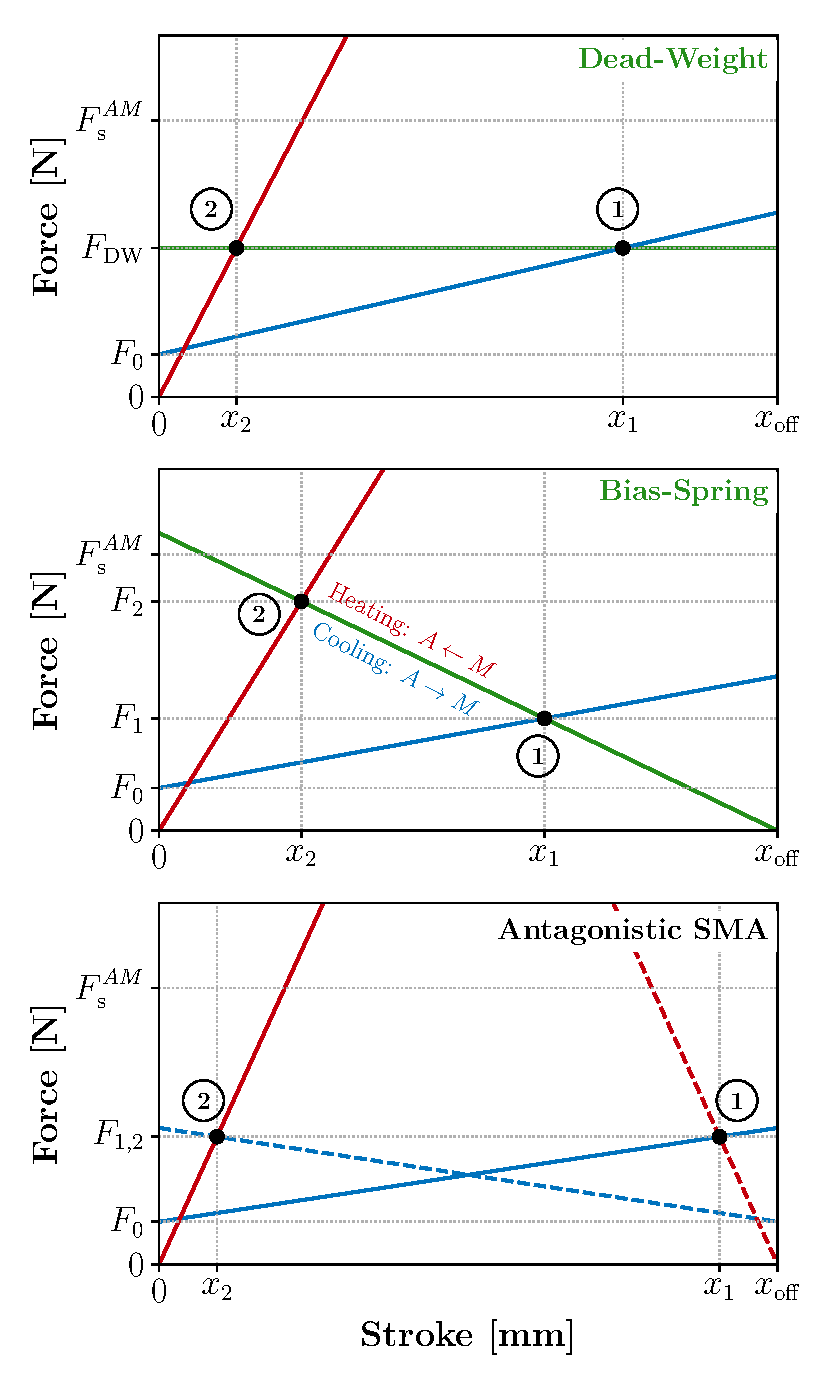
\includegraphics[width=0.65\textwidth]{images/chap2/simplied-sma-bias-all-wp.pdf}

    \begin{tabular}{l@{ }l l@{ }l}
      {\color{myred} \rule[2pt]{10pt}{0.5mm} } & {\footnotesize SMA at $T\uparrow$} & {\color{myblue} \rule[2pt]{10pt}{0.5mm} } & {\footnotesize SMA at $T\downarrow$}\\
    \end{tabular}
    \caption{The simplified sizing methodology of an SMA actuators. Here, the force-displacement characteristics of the SMA are simplified adapted from the work by \cite{dragoniDesignDevelopmentAdvanced2021}.}
    \label{fig:simplied-sma-bias-spring-wp}
\end{figure}

The A phase of the SMA occurs when the material is heated above its transition temperature, $\Af$ and reverts back to the M phase when the temperature drops back down below the martensitic transition temperature, $\Mf$. However, as shown in \cref{fig:phase-diagram-graph}, there is a relationship between the stress imposed on the alloy and its transition temperatures. This implies that that when sufficiently above a certain critical stress threshold, $\sigma_\mathrm{s}^{AM}$, the A phase SMA will revert back to the M phase reducing the rigidity of the material. As the SMA actuator operates by the change in material rigidity between the high temperature and low temperature phases, this change in rigidity at the critical stress threshold will cause the actuator to have a reduced stroke. Thus, when designing SMA actuators, this maximum stress or force output must be taken into account using \cref{eq:critical-M-stress}. In the case, the biasing element exceeds this critical stress, the final stroke of the material is greatly reduced as the material will be operating within its super-elastic region.

\begin{equation}\label{eq:critical-M-stress}
    \sigma_\mathrm{s}^{AM} = C_M (T-\Ms)
\end{equation}

In this work, SMA helical springs are used due to their availability and the large stroke requirement. The material properties was obtained experimentally and by curve-fitting the resulting force-displacement profile. In this case, a PID controller paired with a thermal camera as a feedback is used to maintain the SMA spring at a constant temperature. A pull-tester is used to elongate the spring while measuring the force to obtain the force-displacement profiles at the required constant temperature. These isothermal traction tests are then curve fitted to obtain the material properties in the M and A phases. Finally, these simplified curves can be used to size the SMA-powered actuators.

While the behaviour of the shape memory effect in these springs is still non-linear, the simplified linearised curves can be used to obtain the operating points of SMA actuators as shown in \cref{fig:simplied-sma-bias-spring-wp}. These experimental results show that the simplified curves are able to quite accurately depict the force-displacement behaviours of SMA helical springs. In the following chapters, the force-displacement profiles obtained from the experimental results have been used to size the various SMA-based actuators.

This methodology of using the respective hot and cold force-displacement profiles is a useful approach to sizing and characterizing an SMA actuator. However, when multi-output systems are employed and kinematic stages with complex behaviours are integrated, this methodology must be appropriately adapted so as to accurately size the active SMA element and predict the actuator stroke. In the following chapters, this simplified methodology is adapted and employed in the sizing of more complex and integrated SMA-powered actuators.

\section{Summary and Conclusion}
In this chapter, the thermomechanical behaviour referred to as the shape memory effect has been presented and modelled. Various modelling strategies, such as finite element modelling and analytical modelling, are presented. The models have been used in the scope of predicting the shape memory effect such that actuators powered by these SMAs can be adequately and accurately sized. In the context of traditional SMA actuators, the models have been adapted and described so as to present the traditional design methodology often employed in SMA-based actuators such as the ones presented in \cref{chap:sma-actuator-design}.

The SME occurs due to various microscopic structure changes that occurs during phase transformations as the alloy is subjected to a thermal load. In the first section, the different phase transformations and crystal structure changes are presented and described. By taking into account the presence of different phases and phase transformations, the requirements and conditions required by the SME cycle is presented and described.

In the context of predicting the SME, the \cite{liangConstitutiveModelingShape1990a} analytical model is presented. This 1-dimensional phenomenological model has been able to provide some constitutive equations that describes the transformation of the alloy between the high temperature A phase and the low temperature M phase. This model, widely used in traditional SMA actuator design, has been presented in this chapter. However, this model does not take into account the low rigidity and highly elastic nature of the SMA at low temperatures. The \cite{brinsonOneDimensionalConstitutiveBehavior1993} model, on the other hand, has taken into account the stress induced detwinning process into the phenomenological model and has allowed the model to accurately describe the thermomechanical behaviour of the SMA at low temperatures.

Furthermore, in this chapter, the modelling of SMAs and its shape memory effect using commercial FEM softwares is presented. These softwares make use of the \cite{auricchioRobustIntegrationalgorithmFinitestrain2001} to accurately model the 3-dimensional behaviour of the alloy when subjected to thermal and mechanical loading. The FEM models have enabled designers to predict the behaviour of the SMAs in cases with more complex geometries and in scenarios where the 1D \cite{brinsonOneDimensionalConstitutiveBehavior1993} models are not sufficient. Furthermore, the various material properties required to define the FEM material model has been showcased.

Using the constitutive equations presented in this chapter, the sizing methodology of the SMA actuators are displayed. Using the \cite{brinsonOneDimensionalConstitutiveBehavior1993} model, the stroke of a commonly used biased-spring SMA actuator is estimated. This adapted model, shown in this chapter, uses the change in rigidity between the two phases of the alloy and the force-displacement profiles of the biasing elements to establish operating points for the actuator based on the temperature of the active element. This methodology allows an accurate sizing of the biasing spring and active SMA element such that the resulting actuator can be designed for any application or scenario. The accurate sizing of the SMA allows employing the smallest and most efficient SMA elements so as to create an actuator that has a compact footprint and a high bandwidth.

In many cases, the highly non-linear nature of the SMA renders the sizing of the SMA actuator quite difficult and computational expensive. Furthermore, in the case of SMA helical springs, the resulting force-displacement curve used in the sizing methodology can be linearised without losing too much accuracy in the stroke estimation. This simplified linear model can be extrapolated to other SMA-based actuators so as to obtain a relatively simple sizing methodology that can be used to estimate in the stroke in the various types of simple SMA actuators.

In the case of SMA-powered actuators where the biasing element or the active element are more complex or perform multiple roles using the same structure, this tradition design methodology must be adapted. In the following chapters, this work focuses on adapting the traditional design methodology such that the same principle can be implemented in cases where the actuator has been highly integrated. The following chapters focus on adapting the traditional methodology such that more complex active and biasing elements can be employed while still being able to accurately size each subsystem.

\vspace*{\fill}
\noindent\hrulefill \\
\textbf{\large Publications related to this chapter :}\\

S. Thomas, M. Almanza, and Y. Perriard, \textit{“Design Analysis of a Shape Memory Alloy Bias-Spring Linear Actuator,”} in 2019 12th International Symposium on Linear Drives for Industry Applications (LDIA), Neuchatel, Switzerland, Jul. 2019, pp. 1–5. doi: 10.1109/LDIA.2019.8770987.
